\documentclass[a4print,english,lof,lot]{univpmphdthesis}
\errorcontextlines=9

\RequirePackage[utf8]{inputenc}
\RequirePackage[T1]{fontenc}

\usepackage{lmodern}
\usepackage[cmex10]{amsmath}
\usepackage{amssymb}
\usepackage{subcaption}
\usepackage{multirow}
\usepackage{booktabs}
\usepackage{framed}
\usepackage{algorithm,algpseudocode}
\usepackage{pgfplots,pgfplotstable}
\usetikzlibrary{pgfplots.groupplots}
\usepackage{tabularx}

\usepackage{tikz}
\usetikzlibrary{shapes,arrows}

\usepackage{tkz-kiviat,numprint}
\usetikzlibrary{decorations.pathreplacing, arrows, fit}
\usepackage{hyperref}


\usetikzlibrary{shadows,arrows,fit,shapes,positioning,calc,backgrounds,spy,decorations.markings}
\usetikzlibrary{backgrounds}

\pgfdeclarelayer{background}
\pgfdeclarelayer{foreground}
\pgfsetlayers{background,main,foreground}

\tikzstyle{bk} = [draw, fill=blue!30, text centered, minimum height=2em, text width=7em, minimum width=6em, minimum height=3em, rounded corners, drop shadow]
\tikzstyle{bkFull} = [draw, fill=blue!30, text centered, minimum height=2em, text width=15em, minimum width=20em, minimum height=3em, rounded corners, drop shadow]
\tikzstyle{bkDec} = [draw, fill=red!40, text centered, minimum height=2em, text width=15em, minimum width=15em, minimum height=3em, rounded corners, drop shadow]
\tikzstyle{cy} = [draw, fill=gray!30, text centered, minimum height=3em, text width=7em, minimum width=2em, cylinder, shape border rotate=90, shape aspect=0.1, drop shadow]
\tikzstyle{cyFull} = [draw, fill=gray!30, text centered, minimum height=3em, text width=7em, minimum width=20em, cylinder, shape border rotate=90, shape aspect=0.1, drop shadow, dashed]
\tikzstyle{bg}=[rectangle,fill=gray!30,inner sep=0.2cm,rounded corners,draw=black!50, dashed]
\tikzstyle{input} = [coordinate]

\tikzset{
	myarrow/.style={
		draw,thick,
		single arrow,
		%text width=1cm,
		minimum height=1cm,
		%anchor=west,
		%fill=white
	},
}

\tikzstyle{vecArrow} = [thick, decoration={markings,mark=at position 1 with {\arrow[semithick]{open triangle 60}}},
double distance=1.4pt, shorten >= 5.5pt, preaction = {decorate}, postaction = {draw,line width=1.4pt, white,shorten >= 4.5pt}]

\tikzstyle{innerWhite} = [semithick, white,line width=1.6pt, shorten >= 4.5pt]




\newcommand{\LegendBox}[3][]{%
	\xdef\fitbox{}%
	\coordinate[#1] (LegendBox_anchor) at (#2) ;
	\foreach \col/\item [count=\hi from 0] in {#3} {
		\node[color = \col,draw,thick,
		fill  = \col,
		minimum width  = 5 ex,
		minimum height = 1 ex,
		name=b\hi,
		] at ([yshift=0 ex,xshift=\hi*40 ex]LegendBox_anchor) {};
		\node[anchor=west,xshift=0.1 ex] at (b\hi.east) (c\hi) {\item};
		\xdef\fitbox{\fitbox(c\hi)}
	}%
	\node [fit=\fitbox(LegendBox_anchor), minimum width = 0 ex] {};
}


\newcommand{\chref}[1]{Chapter~\ref{#1}}
\newcommand{\secref}[1]{Section~\ref{#1}}
\newcommand{\subsecref}[1]{Subsection~\ref{#1}}
\newcommand{\apxref}[1]{Appendix~\ref{#1}}

\newcommand{\figref}[1]{\figurename~\ref{#1}}
\newcommand{\tableref}[1]{Table~\ref{#1}}

\newcommand*\rfrac[2]{{}^{#1}\!/_{#2}}


\def\N{{\mathbb{N}}}
\def\Z{{\mathbb{Z}}}
\def\R{{\mathbb{R}}}

%%%%%%%%%%%%%%%%%%%%%%%%%%%%%%%%%%%%%%%%%%%%%%%%%%%%%%%%%%%
% Metadata
%%%%%%%%%%%%%%%%%%%%%%%%%%%%%%%%%%%%%%%%%%%%%%%%%%%%%%%%%%%
\phdschool{Scuola di Dottorato di Ricerca in Scienze dell'Ingegneria}
\phdfaculty{Facolt\`{a} di Ingegneria}
\phdcurriculum{Curriculum in Ingegneria Elettronica, Elettrotecnica e delle Telecomunicazioni}
\phdtitle{Deep Learning for Sound Event Detection and Classification}
%\phdsubtitle{con questa bellissima classe} % NON NECESSARIO
\phdauthor{Fabio Vesperini}
\phdadvisor{Prof.~Stefano Squartini}
%\phdcoadvisor{Prof.~Michele Blu} % IN TEORIA NON E' AMMESSO
\phdcurriculumadvisor{Prof.~Francesco Piazza}
\phdcycle{17}
\thesisdedication{alla mia famiglia}
\phdlocation{Ancona}
\phdtime{Ottobre 2018}
%%%%%%%%%%%%%%%%%%%%%%%%%%%%%%%%%%%%%%%%%%%%%%%%%%%%%%%%%%%

% Solo per generare testo...
\usepackage{lipsum}

\begin{document}

%%%%%%%%%%%%%%%%%%%%%%%%%%%%%%%%%%%%%%%%%%%%%%%%%%%%%%%%%%%
% Front matter contents
%%%%%%%%%%%%%%%%%%%%%%%%%%%%%%%%%%%%%%%%%%%%%%%%%%%%%%%%%%%
\frontmatter

\maketitle

%\begin{thesisacknowledge}
%\lipsum[1-2]
%\end{thesisacknowledge}

%\begin{thesisacknowledge}[italian]
%\lipsum[1-2]
%\end{thesisacknowledge}

\begin{thesisabstract}
\lipsum[1-3]
\end{thesisabstract}

\thesistoc

%%%%%%%%%%%%%%%%%%%%%%%%%%%%%%%%%%%%%%%%%%%%%%%%%%%%%%%%%%%
% Main matter contents
%%%%%%%%%%%%%%%%%%%%%%%%%%%%%%%%%%%%%%%%%%%%%%%%%%%%%%%%%%%
\mainmatter

\graphicspath{{1_introduction/}}
\chapter{Introduction}\label{ch:intro}

Human cognition relies on the ability to sense, process, and understand the surrounding environment and its sounds.
Although the skill of listening and understanding their origin is so natural for living beings, it still results in a very challenging task for computers. In recent years several novel methods have been proposed to analyze this information automatically, and several new applications have emerged \cite{virtanen2018computational}. However, the creation of ``machine listening'' algorithms that can mimic this cognitive feature by means of artificial systems remains a very challenging task. 

Automatic sound event detection (SED), also known as acoustic event detection, is nowadays considered as one of the most important topics in the field of computational auditory scene analysis (CASA). Thanks to works like Bregman's ``Auditory Scene Analysis: The Perceptual Organization of Sound''~\cite{bregman1994auditory}, we can trace back the birth of this field to 1994, when the field of auditory scene analysis (ASA) was introduced in order to model humans' sound perception. Following this work, many other contributions were written aiming to describe how artificial systems can be designed in order to perceive sounds similarly to as humans do; most of these works will be later collected in Divenyi's book~\cite{divenyi2004speech} in 2004.

Nowdays, one of the main subject of interest in technological research regards systems deployed for surveillance applications. Surveillance can be seen as control of public safety or as the supervision of private environments where people may live alone. 
In fact, the increasing level of public security over the past decades has motivated the installation of sensors such as cameras or microphones in public places (stores, subway, airports, etc.), while is possible to effectively consider personal multimedia devices (smartphones, tablets, etc.) as virtual assistant which is able to monitor the user and eventually intervene in case of necessity without having the need for a physical interface (i.e., keyboard) anymore.
Thus, the need of unsupervised situation assessment stimulated the signal processing community towards experimenting with several automated frameworks, due to their potential in several engineering applications.

In these contexts, sound or sound sensing can be advantageous with respect to other modalities of multimedia processing.  
This is the case of acoustic surveillance \cite{crocco2016audio}, healthcare monitoring \cite{peng2009healthcare, foggia2015reliable} or urban sound analysis \cite{salamon2017deep}, where the short duration of certain events (i.e., a human fall, a gunshot or a glass breaking) or the personal privacy motivate the exploitation of the audio information rather than, e.g., the image processing. 
In addition, audio processing is often less computationally demanding compared to other multimedia domains, thus embedded devices can be easily equipped with microphones and sufficient computational capacity to locally process the signal captured. 
These could be smart home devices for home automation purposes or sensors for wildlife and biodiversity monitoring (i.e., bird calls detection \cite{grill2017two}). 
Some of these applications have already become commercial products that are able recognize certain specific sound categories in realistic environments and improve home security \cite{audioanalytic}  or companies with as much impactful missions, such as preserve the Rainforest from illegal deforestation \cite{rainforest}.

The type of information to be extracted with these algorithms depends on the application. In particular, we can sort the sound analysis tasks explored in this work into two high-level categories: sound event \textit{detection} and sound event \textit{classification}.
In sound event detection (SED), or acoustic event detection, the goal is to detect the onset and offset times for a variety of sound events captured in an audio recording. 

In sound event classification, the goal is to categorize an audio recording into one of a set of predefined categories by associating a textual descriptor.

In controlled laboratory conditions where the data used to develop computational sound scene and event analysis methods matches well with the test data, it is possible to achieve relatively high accuracies in the detection and classification of sounds.  However, there are several complexities in computational sound analysis and current technologies face many challenges, mainly related to the acoustics of sound scenes and events, when they are employed in realistic environments.
Among these challenges we can include:
\begin{itemize}
	\item the effect of the environment acoustics: reverberation, background noises and the channel coupling (impulse response) between the source and the recording equipment;
	\item the intra-class variability, i.e., high difference of the acoustic characteristics of even a single class of sounds and on the other hand the similarity of many different types of sounds to the target events  \cite{stowell2015acoustic};
	\item the \textit{polyphony}, i.e. the occurrence of multiple simultaneous events. In realistic environments there
are almost always multiple sources producing sound at the same time. 
\end{itemize}

In addition to these complications related to the acoustics of sound scenes and
events, there are also several fundamental limitations related to the computational methods. In particular, to develop effective models based on the \textit{deep learning} paradigm, a very large set of examples of the
target (and non-target) sounds is required. In contrast to the situation in image classification,
 currently available datasets that can be used to train such systems are more limited in size, diversity, and number of event
 instances, even though recent contributions such as AudioSet \cite{gemmeke2017audio} or the DCASE challenges
and related workshops \cite{DCASE2017Workshop, mesaros2016tut, dcase2018web} have provided public available datasets to reduce this gap.



\section{The Deep Learning Approach for Sound Event Detection and Classification}

\begin{figure}[b]
	\centering
	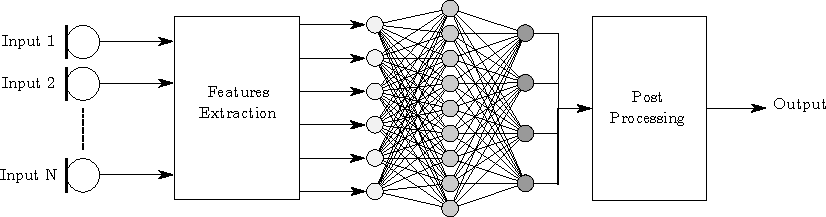
\includegraphics[width=\linewidth]{img/flowchart_1.pdf}
	\caption[Basic structure]{Basic structure of an audio analysis system.}
	\label{fig:base-system}
\end{figure}

\begin{figure}[tb]
	\centering
	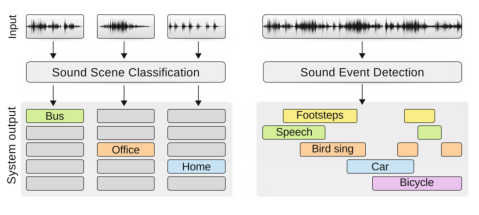
\includegraphics[width=\linewidth]{img/sed_sec.pdf}
	\caption[System input and output ]{System input and output for the two main analysis systems: sound scene classification and sound event detection.}
	\label{fig:system-io}
\end{figure}

The typical computational sound scene
or event analysis system based on machine learning is
depicted in \figref{fig:base-system}, while the different input and output respectively for classification and detection systems
are illustrated in \figref{fig:system-io}.

As the first stage, all the systems take as input one or more audio
signals, either in real-time, captured by a microphone, or offline, from an
audio recording. In this work, we assume always discrete-time signals,
obtained by using analog-to-digital converters. 

The \textit{Feature Extraction} block consists
of different processing stages and outputs acoustic features, as the actual analysis of
audio is rarely based on the raw audio signal, but rather on the compact signal
representation with features. The purpose of the feature extraction is to obtain
information sufficient for detecting or classifying the target sounds, making the
subsequent modeling stage computationally cheaper and also easier to achieve with
limited amount of development material. Very often the feature extraction procedure is also preceded by the down-mixing the audio signal into a single (mono) channel and re-sampling it into fixed sampling frequency.
Although every application could require a specific set of features able to highlight the discriminating particularities of each data sample, the most common representations used
for audio signals are non-linear representation for magnitudes (power spectra and logarithm) and nonlinear frequency scaling (mel-frequency scaling). 
More details of the acoustic features extraction process for each examined case-study will be provided in further chapters.


The \textit{Deep Learning}-based model takes the acoustic features as input and it is trained to produce an output which will assign a class label depending on the application. Almost all the system presented in this work are based on the supervised machine learning approach, where the system is trained using labeled examples of sounds from each of target sound type. 
At the development stage, the obtained acoustic features are used together with
reference annotations of the audio training examples, to learn models for the
sound classes of interest. Annotations contain information about the presence of
target sound classes in the training data, and are used as a reference information
to automatically learn a mapping between acoustic features and class labels. The
mapping is represented by acoustic models. The learning process consists in updating the parameters or \textit{weights} of the neural network, searching for the optimal model that minimize a certain cost-function. 
At the usage stage, the learned acoustic models are used to do recognition (detection or classification), which predicts labels
for the input audio. The recognition stage may also involve temporal models and
post-processing of labels.


After a prediction is obtained through the trained acoustic model, the \textit{Post Processing} stage translates this signal into the effective activity information for each class. Very often this relies on a simple \textit{thresholding} operation or on the selection of the most probable class.


\section{State of the Art}

Traditionally, the computational acoustic event analysis has been approached with statistical modelling methods, including Hidden Markov Models (HMM) \cite{degara2011onset}, Gaussian Mixture Models (GMM) \cite{heittola2010audio}, Non-negative Matrix Factorization (NMF) \cite{carabias2011musical} and support vector machines (SVM) \cite{guo2003content}. 

In the recent era of the ``Deep Learning'', different neural network architectures have been successfully used for sound event detection and classification tasks, including feed-forward neural networks (FNN) \cite{mcloughlin2015robust}, deep belief networks \cite{mohamed2012acoustic}, convolutional neural networks (CNNs) \cite{piczak2015environmental} and Recurrent Neural Networks (RNNs) \cite{graves2013speech}. In addition, these architectures laid the foundation for end-to-end systems \cite{trigeorgis2016adieu, wu2017end}, in which the feature representation of the audio input is automatically learnt from the raw audio signal waveforms. 

The use of deep learning models has been motivated by the increased availability of datasets and computational resources and resulted in significant performance improvements, outperforming in most of the cases the human accuracy \cite{sailor2017unsupervised}.
The methods based on CNNs and RNNs have established the new state-of-the-art performance on the sound event detection task (SED), thanks to the capabilities to learn the non-linear relationship between time-frequency features of the audio signal and a target vector representing sound events. In \cite{espi2015}, the authors show how ``local'' patterns can be learned by a CNN and can be exploited to improve the performance of detection and classification of non-speech acoustic events occurring in conversation scenes, in particular compared to a FNN-based system which processes multiple resolution spectrograms in parallel. 

This success is a result of close academic-industrial collaboration, which started from the speech or speaker recognition task and extended to the analysis of non-speech, music and sound scenes and events. The combination of the CNN structure with recurrent units has increased the detection performance by taking advantage of the characteristics of each architecture. This is the case of convolutional recurrent neural networks (CRNNs) \cite{cakir2017convolutional}, which provided state-of-the-art performance especially in the case of polyphonic SED. CRNNs consolidate the CNN property of local shift invariance with the capability to model short and long term temporal dependencies provided by the RNN layers. This architecture has been also employed in almost all of the most performing algorithms proposed in the last editions of research challenges such as the IEEE Audio and Acoustic Signal Processing (AASP) Challenge on  Detection and Classification of Acoustic Scenes and Events (DCASE) \cite{DCASE2017Workshop}. 

On the other hand, if the datasets are not sufficiently large, problems such as overfitting can be encountered with these models, which typically are composed of a considerable number of free-parameters (i.e., more than 1M). 

Encouraging polyphonic SED performance have been obtained using CapsNets in preliminary experiments conducted on the Bird Audio Detection task in occasion of the DCASE 2018 challenge \cite{vesperini2018capsule}, confirmed by the results reported in \cite{iqbal2018capsule}.
The CapsNet \cite{sabour2017dynamic} is a recently proposed architecture for image classification and it is based on the grouping of activation units into novel structures introduced in \cite{hinton2011transforming}, named \textit{capsules}, along with a procedure called dynamic routing. The capsule has been designed to represent a set of properties for an entity of interest, while dynamic routing is included to allow the network to implicitly learn global coherence and to identify part-whole relationships between capsules.


%TODO EXTEND SoA ?
%Labels extracted with a SED system usually allow us to achieve a better insight of the considered acoustic scenario, for example they can be used as mid-level representation useful for other CASA research areas. In~\cite{chu2009environmental, heittola2010audio}, for example, authors make use of SED for designing audio context recognition systems, while in~\cite{shah2012lifelogging} and~\cite{wichern2010segmentation} SED is exploited for automatic tagging and audio segmentation respectively. Moreover, SED also found many direct applications in a variety of scenarios, some examples being context-based indexing and retrieval in multimedia databases~\cite{xu2008audio}, unobtrusive health monitoring~\cite{peng2009healthcare}, and audio-based surveillance~\cite{harma2005automatic, crocco2014surveillance, Principi2016a}.
%As we can notice from~\cite{heittola2010audio, peng2009healthcare}, hidden Markov models (HMMs) have been widely used in the literature with the purpose of modelling acoustic events in a SED system, usually in terms of a Gaussian mixture model (GMM). In recent years, new approaches to SED have been proposed, marking a distinct trend towards the use of artificial neural networks (ANNs)-based systems. An interesting comparison between computational costs of different systems is carried out in~\cite{sigtia2016automatic} highlighting that ANNs are able to achieve top performance at the cost of being the most computationally expensive approach. A brilliant example of such performance is given in~\cite{hershey2016cnn}, where different ANNs are trained on a big video dataset and then used for different scopes, among which also SED. For a wider overview of the most recent and powerful SED techniques the reader can refer to the comprehensive analysis carried out by Sharan \emph{et al.}\ in~\cite{sharan2016overview}.

%%%%%%%%%%%%%%%%%%%%%%%%%%%%%%%%%%%%%%%%%%%%%%%%%%%%%%%%%%%%%%%%%%%%%


%The use of deep learning models has been motivated by the increased availability of datasets and computational resources and resulted in significant performance improvements.
%The methods based on CNNs and RNNs have established the new state-of-the-art performance on the SED task, thanks to the capabilities to learn the non-linear relationship between time-frequency features of the audio signal and a target vector representing sound events. In \cite{espi2015}, the authors show how ``local'' patterns can be learned by a CNN and can be exploited to improve the performance of detection and classification of non-speech acoustic events occurring in conversation scenes, in particular compared to a FNN-based system which processes multiple resolution spectrograms in parallel. 

%The combination of the CNN structure with recurrent units has increased the detection performance by taking advantage of the characteristics of each architecture. This is the case of convolutional recurrent neural networks (CRNNs) \cite{cakir2017convolutional}, which provided state-of-the-art performance especially in the case of polyphonic SED. CRNNs consolidate the CNN property of local shift invariance with the capability to model short and long term temporal dependencies provided by the RNN layers. This architecture has been also employed in almost all of the most performing algorithms proposed in the recent editions of research challenges such as the DCASE \cite{DCASE2017Workshop}. On the other hand, if the datasets are not sufficiently large, problems such as overfitting can be encountered with these models, which typically are composed of a considerable number of free-parameters (i.e., more than 1M). 



\section{Case studies}
In this work, different application of deep learning for computational audio models in real environments are analyzed. They are evaluated and compared with state-of-the-art methods on different databases, some of these resulting novel approaches. The broad and extensive experimental evaluations highlight the advantages provided by the acoustic models based on deep learning.

The addressed tasks are the following:
\begin{itemize}
	\item Sound event \textit{Classification}:
	\begin{itemize}
		\item Snore sounds excitation localization;
		\item Acoustic road surface roughness classification;
		\item Bird audio detection;
	\end{itemize}
	\item Sound event \textit{Detection}:
	\begin{itemize}
		\item Overnight snore sound detection;
		\item Rare sound event detection;
		\item Voice activity detection in multiroom environments;
	\end{itemize}
	\item \textit{Polyphonic} Sound event Detection:
	\begin{itemize}
		\item A neural network approach for sound event detection in real life audio;
		\item Polyphonic sound event detection by using CapsNets		
	\end{itemize}
\end{itemize}






\graphicspath{{2_background/}}
\chapter{Background}\label{ch:backg}

The Computers are able to perform complex calculus operations in a short amount of time.
However computers cannot compete with humans in dealing with: common sense, ability to recognize people, objects, sounds, comprehension of natural language, ability to learn, categorize, generalize.

Therefore, why does the human brain show to be superior w.r.t common computers for these kind of problems?
Is there any chance to mimic the mechanisms characterizing the way of working of our brain in order to produce more efficient machines?

In the field of signal analysis, the aim is the characterization of such real-world signals in terms of \textit{signal models}, which can provide the basis for a theoretical description of a signal processing system. They are potentially capable of letting us learn a great deal about the signal source, without having to have the source available.

The ``Deep Learning'' is a new area of machine learning
research, which has been introduced with the objective of moving
Machine Learning closer to one of its original goals: Artificial Intelligence. Deep Learning is about learning multiple levels of
representation and abstraction that help to make sense of data
such as images, sound, and text.

Therefore, in this chapter a theoretical description of the principal Deep Neural Network (DNN) architectures is given. In addition, the algorithms used for their parameter estimation are described, with a focus on the most widely model structure used in the field of the computational acoustic event analysis.


\subsection{Deep Neural Network architectures for for Analysis of Sound Scenes and Events}

%\textbf{ndRob} to complete, 3 pages with figures
%\begin{itemize}
%\item formula (notazione matriciale) del calcolo output di ogni rete
%\end{itemize}

A \textit{biological Neural Networks} is a big set of specialized cells (\textit{neurons}) connected among them, which memorize and process information, thus controlling the body activities they belong to.

\begin{figure}[t]
\centering
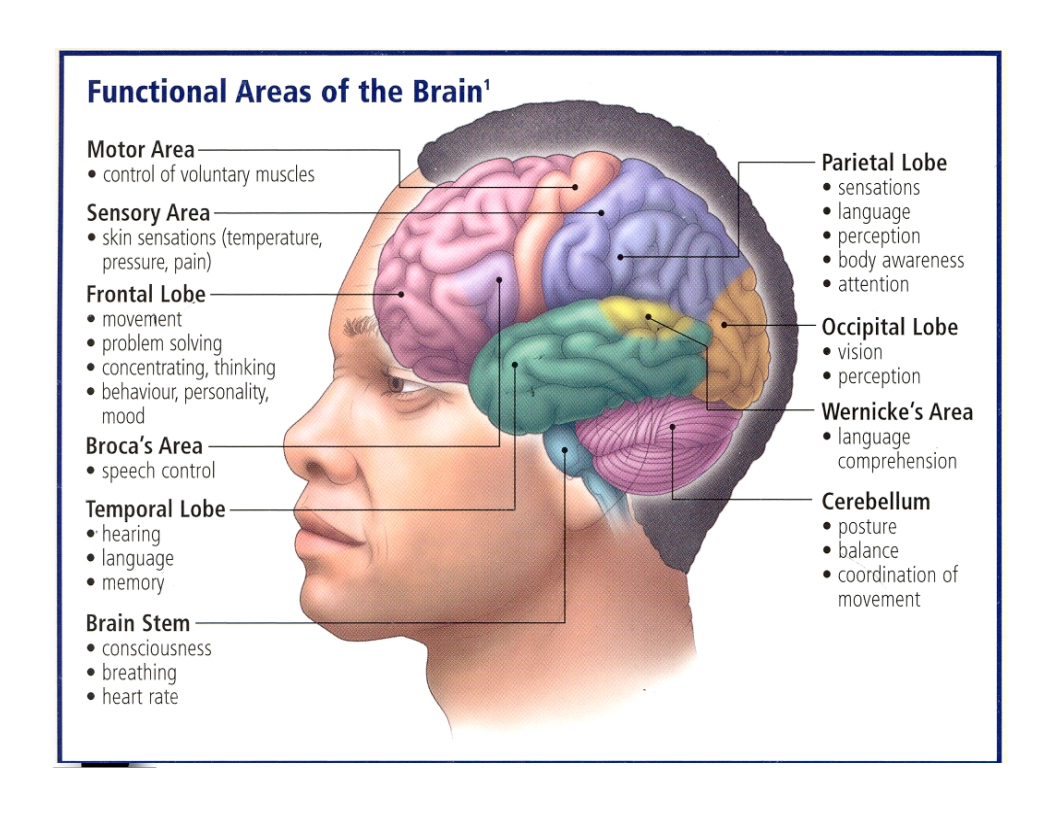
\includegraphics[width=0.65\linewidth]{img/Brain}
\caption{The human brain.}
%\label{vv}
\end{figure}

The \textit{neuron} model is composed of:
\begin{itemize}
\item DENDRITE: input terminal
\item CELL BODY (Nucleus): processing core
\item AXON: output way-out
\item SYNAPSES: output terminal (with weight)
\end{itemize}

%The Biological neurons are electro-chemical devices, operating at low rates ($\approx mses$).
%Digital circuits operate at very high rates ($\approx nsec$).

\begin{figure}[t]
\centering
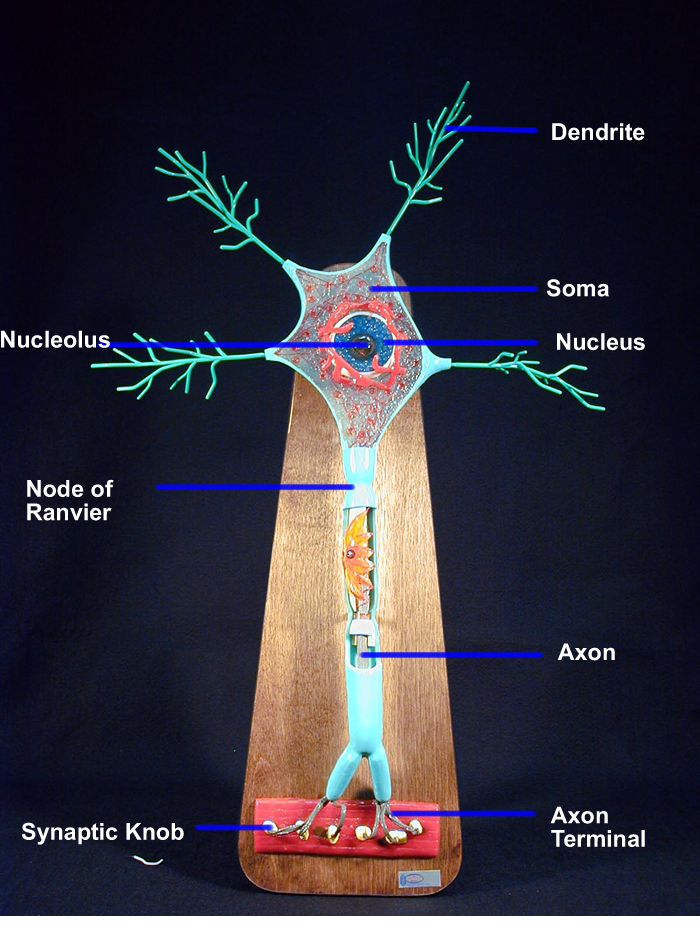
\includegraphics[width=0.4\linewidth]{img/neuron_model}
\caption{The neuron model.}
%\label{aa}
\end{figure}

The \textit{neuron} properties can be described in:
\begin{itemize}
\item LOCAL SIMPLICITY: the neuron receives stimuli (excitation or inhibition) from dendrites and produces an impulse to the axon which is proportional to the weighted sum of the inputs;
\item GLOBAL COMPLEXITY: the human brain possess 
$\mathcal{O}(10^{10})$ 
neurons, with more than 10K connections each;
\item LEARNING: even though the network topology is relatively fixed, the strength of connections (synaptic weights) can change when the network is exposed to external stimuli;
\item DISTRIBUTED CONTROL: no centralized control, each neuron reacts only to its own stimuli;
\item TOLERANCE TO FAILURES: performance slowly decrease with the increase of failures.
\end{itemize}

The biological Neural Networks are able to solve very complex tasks in few time instants (like memorization, recognition, association, and so on.)

\begin{figure}[t]
\centering
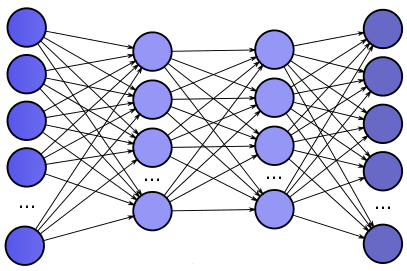
\includegraphics[width=0.4\textwidth]{img/ANN}
\caption{The Artificial Neural Network.}
%\label{aa}
\end{figure}

The \textit{Artificial Neural Networks} (ANNs) are defined as \textit{Massively parallel distributed processors made up of simple processing units having a natural propensity for storing experiential knowledge and making it available for use} (Haykin, 2008).

An ANN resembles the brain in two aspects:
\begin{enumerate}
\item Knowledge is acquired by the network from its environment through a learning process;
\item Synaptic weights are used to store the acquired knowledge.
\end{enumerate}

A \textit{neuron} is an information-processing unit that is fundamental to the operation of a neural network.
The model of a neuron is composed of three basic elements of the neural model:
\begin{itemize}
\item a \textit{set of synapses}, or connecting links, each of which is characterized by a weight or strength of its own, $w_{kj}$;
\item an \textit{adder} for summing the input signals, weighted by the respective synaptic strengths of the neuron; the operations described here constitute a linear combiner;
\item an \textit{activation function} for limiting the amplitude of the output of a neuron. Typically, the normalized amplitude range of the output of a neuron is written as the closed unit interval [0,1], or, alternatively, [-1,1].
\end{itemize}
The neural model also includes an externally applied \textit{bias}, denoted by $b_k$.

\begin{figure}[t]
\centering
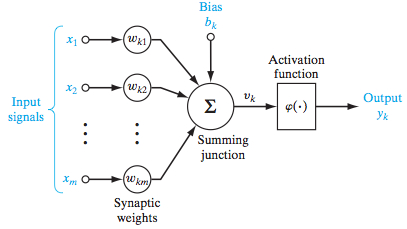
\includegraphics[width=0.8\linewidth]{img/NeuronModel.jpg}
%\label{aa}
\caption{The artificial neuron model.}
\end{figure}

Therefore, the mathematical description of neuron activity can be defined as:
\begin{eqnarray}
{ u }_{ k }=\sum _{ j=1 }^{ m }{ { w }_{ kj } } { x }_{ j }\\ 
{ y }_{ k }=\varphi \left( { u }_{ k }+b_{ k } \right)
\end{eqnarray}
where:
\begin{itemize}
\item ${ x }_{ 1 },{ x }_{ 2 },\cdots ,{ x }_{ m }$ are the input signals;
\item ${ w }_{ k1 },{ w }_{ k2 },\cdots ,{ w }_{ km }$ are the respective synaptic weights of neuron $k$;
\item $u_k$ is the linear combiner output due to the input signals;
\item $b_k$ is the bias;
\item $\varphi(\cdot)$ is the activation function;
\item $y_k$ is the output signal of the neuron.
\end{itemize}

The types of \textit{activation non-linear functions} $\varphi(x)$ are:
\begin{itemize}

\item the \textit{threshold function}: in engineering, this form of a threshold function is commonly referred to as a Heaviside function;
\begin{eqnarray}
\varphi \left( v \right) =1\quad if\quad v\ge 0 \\ 
\varphi \left( v \right) =0\quad if\quad v<0
\end{eqnarray}
\begin{figure}
\centering
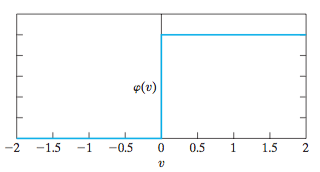
\includegraphics[width=0.4\textwidth]{img/Heaviside}
\caption{The threshold non-linear function.}
%\label{aa}
\end{figure}

\item the \textit{sigmoid function}: it is defined as a strictly increasing function that exhibits a graceful balance between linear and nonlinear behavior; an example of the sigmoid function is the \textit{logistic function} defined by:
\begin{equation}
\varphi \left( v \right) =\frac { 1 }{ 1+exp\left( -av \right)  } 
\end{equation}
\begin{figure}
\centering
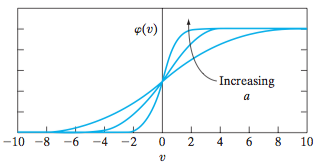
\includegraphics[width=0.4\textwidth]{img/sigmoid}
\caption{The sigmoid non-linear function.}
%\label{aa}
\end{figure}

\item the \textit{ hyperbolic tangent } ($tanh$): it is simply a scaled and shifted version of the sigmoid function:
\begin{equation}
\varphi(x) = \frac{1-e^{-2x}}{1+e^{-2x}}
\end{equation}
\begin{figure}[t]
\centering
	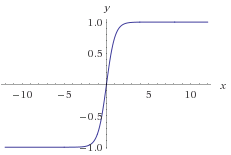
\includegraphics[width=0.4\textwidth]{img/tanh}
	\caption{The $tanh$ non-linear function.}
%				\label{aa}
\end{figure}

\item the \textit{ Rectifier Linear Unit} ($ReLU$):
\begin{equation}
\varphi(x) = \text{max}(0,x)
\end{equation}
\begin{figure}[t]
\centering
	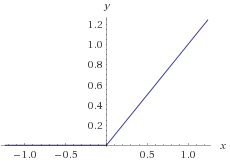
\includegraphics[width=0.4\textwidth]{img/relu}
	\caption{The $ReLU$ non-linear function.}
%				\label{ee}
\end{figure}

\item the $softmax$: it is used on the last layer of a classifier setup: the outputs of the softmax layer represent the probabilities that a sample belongs to the different classes. Indeed, the sum of all the output is equal to $1$.
			%In this case the targets are \textit{one-hot} vectors and the cost-function is the \textit{categorical cross-entropy}.
\begin{equation}
\varphi(x_k) = \frac{e^{x_k}}{\sum_{j=1}^{N}e^{x_j}} \text{ for }  k=1,\dots,K
\end{equation}
\begin{figure}[t]
\centering
	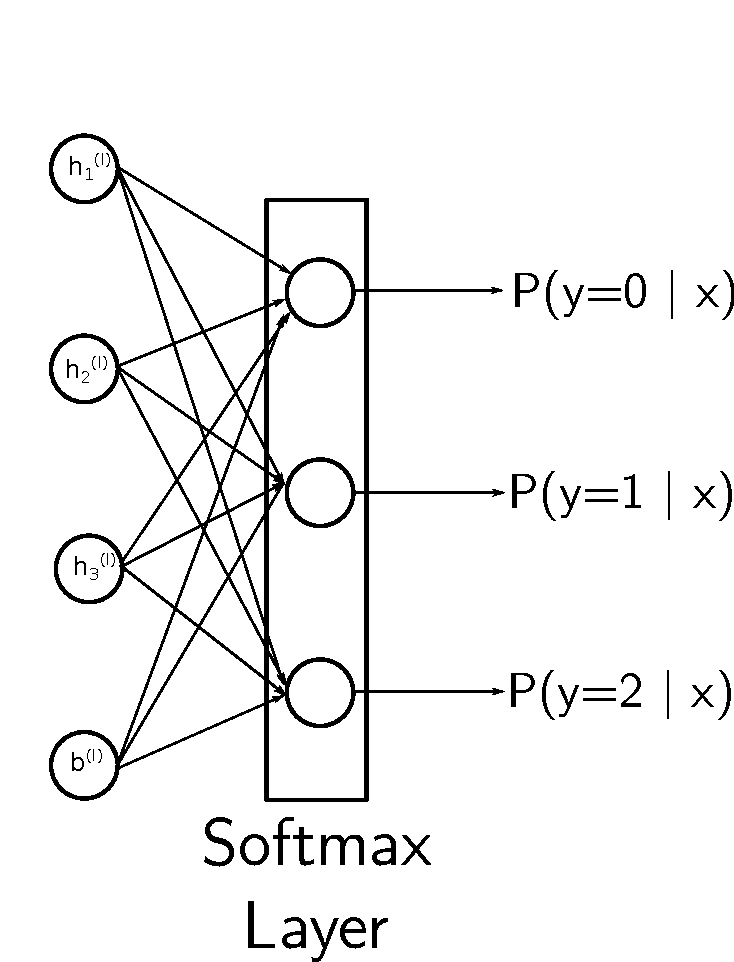
\includegraphics[width=0.4\textwidth]{img/softmax}
	\caption{The $\textit{softmax}$ layer in a neural network classifier.}
%					\label{aa}
\end{figure}	
			
%			\item $\mathbf{maxout}$ - the output is the maximum value among $K$ linear models applied to a given input (or an hidden activation): $\varphi(x_k) = \max(x_k)$ with $k=1,\dots,K$.\\
%			It is supposed to be combined with dropout.
			
	%		It is an approximate model averaging technique. A single maxout unit performs a piecewise linear approximation to an arbitrary convex function. Maxout networks learn not just the relationship between hidden units, but also the activation function of each hidden unit.	
		
				
		
%				\begin{figure}
%				\centering
%					\includegraphics[width=0.75\textwidth]{img/maxout}
%					\caption{Example of an MLP with $\mathbf{maxout}$ units. Picture courtesy of GoodFellow et al. 2013}
%%					\label{rr}
%				\end{figure}

\end{itemize}

% ****************************************************+
%NEURAL NETWORKS VIEWED AS DIRECTED GRAPHS
%
%A neural network is a \textbf{directed graph} consisting of nodes with interconnecting synaptic and activation links and is characterized by four properties:
%
%\begin{enumerate}
%\item Each neuron is represented by a set of linear synaptic links, an externally applied bias, and a possibly nonlinear activation link. The bias is represented by a synaptic link connected to an input fixed at $+1$.
%\item The synaptic links of a neuron weight their respective input signals.
%\item The weighted sum of the input signals defines the induced local field of the neuron in question
%\item The activation link squashes the induced local field of the neuron to produce an output
%\end{enumerate}
%
%\begin{figure}
%\centering
%\includegraphics[width=0.55\textwidth]{img/NeuronGraph.jpg}
%\caption{The Neuron graph model.}
%%\label{key}
%\end{figure}
%
%When the focus of attention is restricted to signal flow from neuron to neuron, we may use a reduced form of this graph by omitting the details of signal flow inside the individual neurons. Such a directed graph is said to be \textit{partially complete}. It is characterized as follows:
%
%\begin{enumerate}
%\item Source nodes supply input signals to the graph.
%\item Each neuron is represented by a single node called a computation node.
%\item The communication links interconnecting the source and computation nodes of the graph carry no weight; they merely provide directions of signal flow in the graph.
%\end{enumerate}
%
%%\begin{figure}
%%\centering
%%\includegraphics[width=0.55\textwidth]{img/NeuronPGraph.jpg}
%%%\label{aa}
%%\caption{ee}
%%\end{figure}
%
%
%Graphical representations of a neural network
%
%\begin{itemize}
%\item \textbf{Block Diagram} $\rightarrow$ functional description of the network
%\item \textbf{Architectural Graph} $\rightarrow$ description of the network layout
%\item \textbf{Signal-Flow Graph} $\rightarrow$ complete description of the signal flow in the network
%\end{itemize}

% *********************************************************+

The manner in which the neurons of a neural network are structured is intimately linked with the learning algorithm used to train the network. % Therefore, the learning algorithms (rules) used in the design of neural networks as being structured.
There, the \textit{network architectures} (structures) is defined.
In general, two different classes of network architectures are identified:
\begin{enumerate}

%\item \textit{Single-Layer Feedforward Networks} (SLFN):
%
%\begin{itemize}
%\item We have an input layer of source nodes that projects directly onto an output layer of neurons (computation nodes), but not vice-versa 
%\item Such a network is called a single-layer network, with the designation \emph{single-layer} referring to the output layer of computation nodes (neurons). 
%\item We do not count the input layer of source nodes because no computation is performed there.
%\end{itemize}
%
%\begin{figure}
%\centering
%\includegraphics[width=0.35\textwidth]{img/SLFN}
%%\label{aa}
%\caption{The Single-Layer Feedforward Network.}
%\end{figure}


\item \textit{Multilayer Feedforward Networks} - (FFNN):

it is characterized by the presence of one or more hidden layers, whose computation nodes are correspondingly called \textit{hidden neurons} (or hidden units);
the term \textit{hidden} refers to the fact that this part of the neural network is not seen directly from either the input or output of the network. 
The function of hidden neurons is to intervene between the external input and the network output in some useful manner. By adding one or more hidden layers, the network is enabled to extract higher-order statistics from its input. 
%\item Example: \textbf{10-4-2 network} $->$ it has 10 source nodes, 4 hidden neurons, and 2 output neurons.


\begin{figure}
\centering
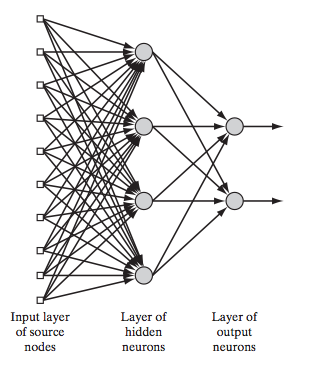
\includegraphics[width=0.4\textwidth]{img/MLP}
%\label{aa}
\caption{The Multilayer Feedforward Network.}
\end{figure}


%\textbf{ndRob} to complete, 1 pages with figure
%\begin{itemize}
%\item struttura a layer
%\item notazione matriciale con indici layer
%\end{itemize}

The MLP is a well known kind of artificial neural network introduced in 1986 \cite{Rumelhart86-LRB}. 
Each node applies an activation function over the weighted sum of its inputs. 
The units are arranged in layers, with feed forward connections from one layer to the next. 
The stochastic gradient descent with error back-propagation algorithm is used for the supervised learning of the network. 
In the forward pass, input examples are fed to the input layer, and the resulting output is propagated via the hidden layers towards the output layer. At the backward pass, the error signal originating at the output neurons is sent back through the layers and the network parameters (i.e., weights and biases) are tuned.

A single neuron can be formally described as:
\begin{equation}
%g(\mathbf{u}[n])=\varphi \left(\left(\begin{matrix} \sum _{ j=1 }^{ D }{w_j u_j[n] }  \end{matrix} \right) + b\right),
g(\mathbf{u}[n])=\varphi \left(\sum _{ j=1 }^{ D }{w_j u_j[n] } + b\right),
\end{equation}
where $\mathbf{u}[n] \in \mathbb{R}^{D\times 1}$, the bias $b$ is an externally applied term and $\varphi(\cdot)$ is the non-linear activation function.
Thus, the mathematical description of a one-hidden-layer MLP is a function $\mathbf{f}:\mathbb{R}^D \rightarrow \mathbb{R}^{D'}$, where $D'$ is the size of the output vector, so:
\begin{equation}
\mathbf{f}(\mathbf{u}[n]) = 	\varphi \left( \mathbf{b}_2 + \mathbf{W}_2 \left( \varphi \left( \mathbf{b}_1 + \mathbf{W}_2 \cdot \mathbf{u}[n]\right) \right) \right),
\end{equation}
where $\mathbf{W}_i$ and $\mathbf{b}_{i}$ are the respective synaptic weights matrix and the bias vector of the $i$-th layer.
The behaviour of this architecture  is  parametrized  by  the connection weights, which are adapted during the supervised network training.



\item \textit{Convolutional Neural Networks}(CNN)

\begin{figure}
	 \centering
	 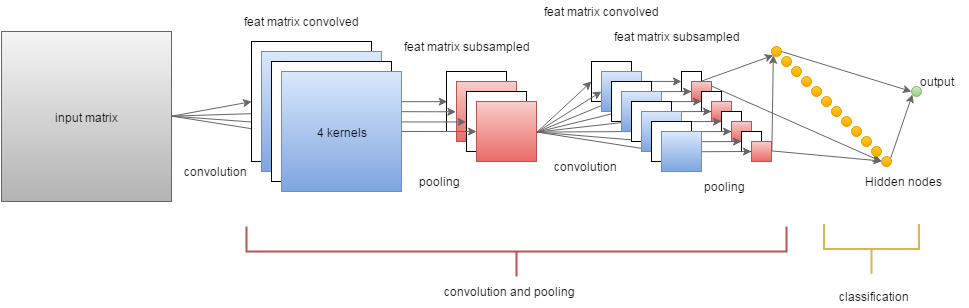
\includegraphics[width=0.9\columnwidth]{img/CNN}
%	 \label{ee}
	 \caption{The Convolutional Neural Network.}
	\end{figure}

%\textbf{ndRob} to complete,  1 pages with figure

Convolutional neural networks are feedforward neural networks similar to multilayer perceptron, with some special layers.

%Matrix convolution: it is performed between a bigger matrix, which is the input, and a smaller matrix, the convolutional kernel.

\begin{figure}[t]
		\centering
		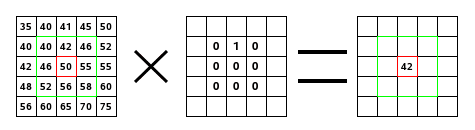
\includegraphics[width=0.7\columnwidth]{img/convolution-calculate}
%		\label{ee}
		\caption{The convolution operation.}
	\end{figure}
	


%	\item Convolution kernels, by training, adapt on recurrent input patterns, becoming themselves similar to those patterns. As a result an activation of the kernel is given when a specific pattern occurs. 
Convolution kernels process the input data matrix by dividing it in \textit{local receptive fields}, a region of the same size of the kernel, and sliding the local receptive field across the entire input.
Each hidden neuron is thus connected to a local receptive field, and all the neurons form a matrix called \textit{feature map}.
%We can have multiple feature maps.
The weights in each \textit{feature map} are \textit{shared}: all hidden neurons are aimed to detect exactly the same pattern just at different locations in the input image. 

The main advantages of this network is the robust pattern recognition system characterized by a strong immunity to pattern shifts.

Pooling layer just reduces the dimension of the matrix by a rule: a submatrix of the input is selected, and the output is the maximum value of this submatrix.
	
	\begin{figure}
		\centering
		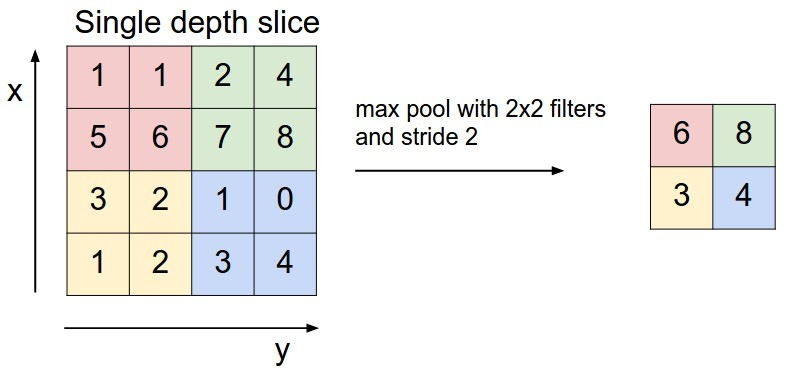
\includegraphics[width=0.6\columnwidth]{img/maxpool.jpeg}
%		\label{rr}
		\caption{The max-pooling layer.}
	\end{figure}

The pooling process introduces tolerance against shifts of the input patterns. Together with convolution layer it allows the CNN to detect if a particular event occurs, regardless its deformation or its position.

CNN is a feed-forward neural network \cite{726791} usually composed of three types of layers: convolutional layers, pooling layers and layers of neurons.
The convolutional layer performs the mathematical operation of convolution between a multi-dimensional input and a fixed-size kernel. Successively, a non-linearity is applied element-wise. 
%In the convolution process the kernel moves all along the input matrix and, for each position, every element of the kernel is multiplied with the corresponding one on the input matrix. All the values are finally summed.
The kernels are generally small compared to the input, allowing CNNs to process large inputs with few trainable parameters.
%From the input matrix, for each convolutional kernel, a new matrix is obtained, also called \textit{feature map}.
Successively, a pooling layer is usually applied, in order to reduce the feature map dimensions. One of the most used is the \textit{max-pooling} whose aim is to introduce robustness against translations of the input patterns.
%Different strategies are available for pooling, but we only consider max-pooling, which selects the maximum value in a sub-matrix of the input and discards the other values. Pooling introduces toughness against shifts of the input patterns. 
Finally, at the top of the network, a layer of neurons is applied. This layer does not differ from MLP, being composed by a set of activation and being fully connected with the previous layer. For clarity, the units contained in this layer will be referred as \textit{Hidden Nodes} (HN).

Denoting with $\mathbf{W}_{m} \in \mathbb{R}^{K_{1m}\times K_{2m}}$ the $m$-th kernel and with $\mathbf{b}_{m}  \in \mathbb{R}^{D_1\times D_2}$ the bias vector of a generic convolutional layer, the $m$-th feature map  $\mathbf{h}_{m} \in \mathbb{R}^{D_1\times D_2}$ is given by:
\begin{equation}\label{eq:backg:dnn:conv_op}
%h_{m,i}=\varphi	\left(W_{m,i} \ast \mathbf{u}_j[n] + b_{m,i} \right),
\mathbf{h}_{m}=\varphi	\left(\sum_{d=1}^{D_3} \mathbf{W}_{m} \ast \mathbf{u}_d + \mathbf{b}_{m} \right),
\end{equation}
where $\ast$ represent the convolution operation, and $\mathbf{u}_{d} \in \mathbb{R}^{D_1\times D_2} $ is a matrix of the three-dimensional input tensor $\mathbf{u} \in \mathbb{R}^{D_1\times D_2 \times D_3}$. The dimension of the $m$-th feature map $\mathbf{h}_{m}$ depends on the zero padding of the input tensor: here, padding is performed in order to preserve the dimension of the input, i.e., $\mathbf{h}_{m} \in \mathbb{R}^{D_1\times D_2}$. Please note that for the sake of simplicity, the time frame index $n$ has been omitted.  %The different feature maps obtained from each kernel of a convolutional layer are then summed to compose the input data for the following layer.
Commonly, \eqref{eq:backg:dnn:conv_op} is followed by a pooling layer in order to be more robust against patterns shifts in the processed data, e.g. a max-pooling operator that calculates the maximum over a $P_1 \times P_2 $ matrix is employed.

\end{enumerate}


A \textit{Deep Learning} definition: \textit{A  class  of  machine learning  techniques  that
exploit  many  layers  of  non-linear  information  processing  for supervised  or  unsupervised  feature  extraction  and  transformation, and for pattern analysis and classification.}
%...we need complex networks to deal with the \textit{feature representation learning} paradigm.
Artificial Neural Networks are often referred as deep when they have more than 1 or 2 hidden layers.
%		\item Important Issues
%		\begin{itemize}
%			\item Rule of Thumb: \textit{for a given performance rate on the testing data, the amount of training data and the number of free parameters are directly proportional}.
%			\item Do we have enough data for training and to achieve a satisfying generalization performance?
%			\item How to select the ``right'' model? 
%		\end{itemize}


\subsection{Stochastic gradient descent (SGD)}

Most deep learning training algorithms involve optimization of some sort.
The most widely used is the gradient based optimization, which belongs to the first order type.

\textit{Optimization} is the task of either minimizing some function $f(x)$ by altering $x$:
$f(x)$ is called \textit{objective function}, but in the case when it has to be minimized, it is also call the \textit{cost function}, \textit{loss function}, or \textit{error function}.
The aim of the optimization is reached doing small change $\epsilon$ in the input $x$, to obtain the corresponding change in the output $f(x)$:
\begin{equation}
f(x+\epsilon) \approx f(x)+\epsilon\,f'(x).
\end{equation}
This formulation is based on the calculation of the derivative $f'(x)$.
The \textit{gradient descent} is the technique based on the reduction of $f(x)$ by moving $x$ in small steps with the opposite sign of the derivative.
The aim is to find the minimum of the cost function: when $f'(x)=0$, the derivative provides no information about which direction to move, therefore this point is defined as stationary points.
A local minimum is a point where $f(x)$ is lower than at all neighbouring and it is no longer possible to decrease $f(x)$ by making infinitesimal steps.
The absolute lowest value of $f(x)$ is a \textit{global minimum}.

For the concept of minimization to make sense, there must still be only one (scalar) output.
For functions that have multiple inputs $f: \R^n \rightarrow \R$, the concept of \textit{partial derivatives} is introduced.
The gradient $\nabla_{\mathbf{x}}f(\mathbf{x})$ is the vector containing all the partial derivatives.

The method of \textit{steepest descent} or \textit{gradient descent} states that decrease $f$ by moving in the direction of the negative gradient.
\begin{equation}
\textbf{x'} = \textbf{x} - \epsilon\,\nabla_{\mathbf{x}}f(\mathbf{x}),
\end{equation}
where $\epsilon$ is the \textit{learning rate}, a positive scalar determining the size of the step.

Large training sets are necessary for good generalization, but large training sets are also more computationally expensive.
The cost function decomposes as a sum over training example of per-example loss function:
i.e., the negative conditional log-likelihood of the training data is defined as:
\begin{equation}
J(\mathbf{\theta}) = \mathbb{E}(L(\textbf{x}, y, \mathbf{\theta})) = \frac{1}{m} \sum\limits_{i=1}^{m} L(\textbf{x}^{(i)}, y^{(i)}, \mathbf{\theta}),
\end{equation}
where $L$ is the per-example loss $L(\textbf{x}, y, \mathbf{\theta}) = - \log p(y|\textbf{x};\mathbf{\theta})$.
The gradient descent requires computing:
\begin{equation}
\nabla_{\theta} J(\mathbf{\theta}) = \frac{1}{m} \sum\limits_{i=1}^{m} \nabla_{\theta} L(\textbf{x}^{(i)}, y^{(i)}, \mathbf{\theta}).
\end{equation}
The computational cost of this operation is proportional to the number of example $m$, therefore as the training set size grows the time to take a single gradient step becomes prohibitively long.

\textit{Stochastic gradient descent} (SGD) is an extension of the gradient descent algorithm: the insight is that the gradient is an expectation estimated using a small set of samples.
On each step of the algorithm, a sample of example $\mathbb{B} = \{ \textbf{x}^{(1)}, \ldots, \textbf{x}^{(m')}\}$, called \textit{minibatch}, is drawn uniformly from the training set.
The minibatch size $m'$ is typically chosen to be a relatively small number of examples.
The estimate of the gradient is:
$\textbf{g} = \frac{1}{m'} \nabla_{\theta} \sum\limits_{i=1}^{m'} L(\textbf{x}^{(i)}, y^{(i)}, \mathbf{\theta})$
using examples from the minibatch $\mathbb{B}$.
The SGD algorithm then follows the estimated gradient downhill:
\begin{equation}
\theta \leftarrow \theta - \epsilon\,\textbf{g}
\end{equation}
where $\epsilon$ is the learning rate.

%\textbf{ndRob} to be inserted: tipo di loss function MSE, come si calcola su uscita 

%\textbf{ndRob} to complete, learning for FF e CNN (in slides)




\subsection{Autoencoder}

%\textbf{ndRob} to complete, 1-2 pages with figures
%
%\begin{itemize}
%\item definition
%\item notazione matriciale
%\item denoising Auto Encoder (dAE)
%\end{itemize}



An Autoencoder is a kind of neural network typically consisting of only one hidden layer, trained to set the target values to be equal to the inputs.
\begin{equation} %\label{eq:layer2}
  \tilde{x} = f(W_{2}h(x) +b_{2})
\end{equation}
 
%\begin{figure}
%\centering
%\includegraphics[width=0.65\textwidth]{img/basic_AE}
%%\label{ee}
%\caption{rr}
%\end{figure}


Given an input set of examples $\mathcal{X}$, autoencoder training consists
in finding parameters $\theta=\{W_{1},W_{2},b_{1},b_{2}\}$ that
minimize the Reconstruction Error:
\begin{equation}\label{eq:obAE}
  \mathcal{J}(\theta)=\sum_{x\in{\mathcal{X}}}\left\| x - \tilde{x}\right\|^{2}
\end{equation}

Defining $M$ the number of hidden units, and $N$ the number of input units, output units, features size:

\begin{figure}
\centering
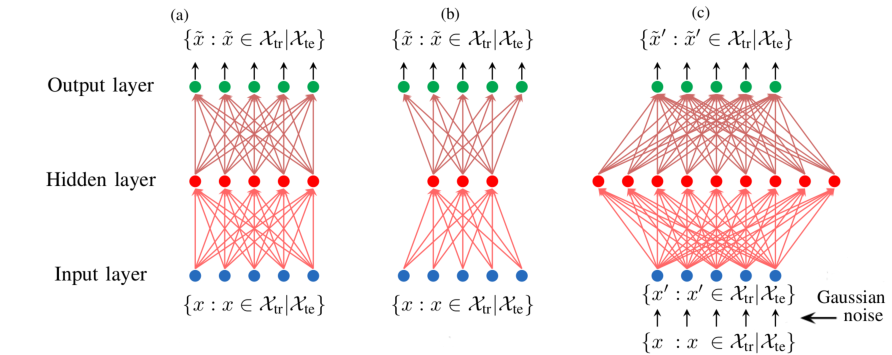
\includegraphics[width=\columnwidth]{img/autoencoders}
\caption{The different types of Autoencoders.}
\label{fig:backg:dnn:AE}
\end{figure}

\begin{itemize}
\item (a):  $M=N \rightarrow$ Basic Autoencoder (AE);
\item (b):  $M<N \rightarrow$ Compression Autoencoder (CAE);
\item (c):  $M>N$ and Gaussian Noise $\rightarrow$ Denoising Autoencoder (DAE);
\end{itemize}


%This section introduces the concepts of autoencoders and describes the basic autoencoder, compression autoencoder, de-noising autoencoder, and non-linear predictive autoencoder.


\subsubsection{Basic Autoencoder}
A basic AE -- a kind of neural network typically consisting of only one hidden layer --, sets the target values to be equal to the input. It is used to find common data representation from the input \cite{Goodfellow2009-MII,Bengio2007-GLT}. Formally, in response to an input example $x\in \mathbf{R}^{n}$, the hidden representation
$h(x) \in \mathbf{R}^{m}$ is 
\begin{equation} %\label{eq:layer1}
  h(x) = f(W_{1}x +b_{1}), 
\end{equation}
where $f(z)$ is a non-linear activation function, typically a logistic
sigmoid function $f(z) = 1/(1+\exp(-z)) $ applied component-wisely,
$W_{1} \in \mathbf{R}^{m \times n}$ is a weight matrix, and $b_{1} \in
\mathbf{R}^{m}$ is a bias vector.

The network output maps the hidden representation $h$ back to a
reconstruction $\tilde{x} \in \mathbf{R}^{n}$:
\begin{equation} %\label{eq:layer2}
  \tilde{x} = f(W_{2}h(x) +b_{2}), 
\end{equation}
where $W_{2} \in \mathbf{R}^{n \times m}$ is a weight matrix, and $b_{2} \in
\mathbf{R}^{n}$ is a bias vector.

Given an input set of examples $\mathcal{X}$, AE training consists
in finding parameters $\theta=\{W_{1},W_{2},b_{1},b_{2}\}$ that
minimise the reconstruction error, which corresponds to minimising
the following objective function:
\begin{equation} %\label{eq:obAE}
  \mathcal{J}(\theta)=\sum_{x\in{\mathcal{X}}}\left\| x -
    \tilde{x}\right\|^{2}.
\end{equation}
The minimisation is usually realised by stochastic gradient descent as
in the training of neural networks. The structure of the AE is given in \figref{fig:backg:dnn:AE}a.   

\subsubsection{Compression Autoencoder}
In the case of having the number of hidden units $m$ smaller than the number of input units $n$, the network is forced to
learn a compressed representation of the input. For example, if some of the input features are correlated, then this compression autoencoder (CAE) is able to learn those correlations and reconstruct the input data from a compressed representation. The structure of the CAE is given in \figref{fig:backg:dnn:AE}b.

\subsubsection{De-noising Autoencoder}\label{sssec:backg:dnn:dAE}
The de-noising AE (DAE) \cite{Vincent10-SDA} forces the hidden layer to retrieve more robust features and prevent it from simply learning the identity. In such a configuration the AE is trained to reconstruct the original input from a corrupted version of it. Formally, the initial input $x$ is corrupted by means of additive isotropic Gaussian noise in order to obtain: $x'|x \sim N(x,\sigma^2I)$. The corrupted input $x'$ is then mapped, as with the AE, to a hidden representation
\begin{equation} %\label{eq:layer11}
  h(x') = f(W'_{1}x' +b'_{1}), 
\end{equation}
from which the original signal is reconstructed as follows:
\begin{equation} %\label{eq:layer12}
  \tilde{x}' = f(W'_{2}x +b'_{2}). 
\end{equation}
The parameters $\theta'=\{W'_{1},W'_{2},b'_{1},b'_{2}\}$ are trained to minimise the average reconstruction error over the training set, to have $\tilde{x}'$ reach as close as possible to the uncorrupted input $x$, which corresponds to minimising the objective function in Equation \ref{eq:obAE}.
%%%%%%%%%%%%%%%%%%%%%%%%%
The structure of the de-noising autoencoder is shown in \figref{fig:backg:dnn:AE}c.





%\textbf{ndRob} descrizione teorica dAE 1D, from paper Neural NILM, 









\graphicspath{{3_datasets_and_evaluation/}}
\chapter{Datasets and Evaluation}\label{ch:datasets}
Every problem to be solved with machine learning and data mining techniques
requires the availability of data for algorithm parametrization: the ability to
access public dataset, representative of a real scenario, allows to test the approaches, in order to evaluate the effective benefit in real applications, and
to compare the performance of existing approaches on a common comparison
basis. A reliable
evaluation procedure for a classification or recognition system will involve a
standard dataset of example input data along with the intended target output, and
well-defined metrics to compare the systems’ outputs with this ground truth. 

%TODO Define typical characteristics of dataset acquisition

\section{Datasets for Sound Event Detection}
In order to evaluate the proposed method in polyphonic real-life conditions, we used the TUT Sound Events 2016 \& 2017 datasets, which were included in the corresponding editions of the DCASE Challenge. For the monophonic-SED case study, we used the TUT Rare Sound Events 2017 which represents the task 2 of the DCASE 2017 Challenge.

\subsubsection{TUT Sound Events 2016}
The TUT Sound events 2016 (TUT-SED 2016)\footnote{\url{http://www.cs.tut.fi/sgn/arg/dcase2016/}} dataset consists of recordings from two acoustic scenes, respectively ``Home'' (indoor) and ``Residential area'' (outdoor) which we considered as two separate subsets. These acoustic scenes were selected from the challenge organizers to represent common environments of interest in applications for safety and surveillance (outside home) and human activity monitoring or home surveillance \cite{mesaros2016tut}.
%The dataset was collected in Finland by Tampere University of Technology from different locations by means of a binaural recording system. For each location, a 3-5 minute long binaural
%audio recording is provided for a total of around 54 and 59 minutes of audio respectively for ``Home'' and ``Residential area'' scenario.
A total amount of around 54 and 59 minutes of audio are provided respectively for ``Home'' and ``Residential area'' scenarios.
Sound events present in each recording were manually annotated without any further cross-verification, due to the high level of subjectivity inherent to the problem. 
For the ``Home'' scenario a total of 11 classes were defined, % (including Object impact, People walking, Washing dishes),
while for the ``Residential Area'' scenario 7 classes were annotated. % (including Bird singing, Car passing by, People speaking).

Each scenario of the TUT-SED 2016 has been divided into two subsets: development dataset and evaluation dataset. The split was done based on the number of examples available for each sound event class. In addition, for the development dataset a cross-validation setup is provided in order to easily compare the results of different approaches on this dataset. The setup consists of 4 folds, so that each recording is used exactly once as test data. In detail, ``Residential area'' sound events data consists of 5 recordings in the evaluation set and 12 recordings in the development set while ``Home'' sound events data consists of 5
recordings in the evaluation set and 10 recordings in turn divided into 4 folds as training and validation subsets.


\subsubsection{TUT Sound Events 2017}
The TUT Sound Events 2017 (TUT-SED 2017)\footnote{\label{note_dcase17}\url{http://www.cs.tut.fi/sgn/arg/dcase2017/}} dataset consists of recordings of street acoustic scenes with various levels of traffic and other activities, for a total of 121 minutes of audio. The scene was selected as representing an environment of interest for detection of sound events related to human activities and hazard situations. It is a subset of the TUT Acoustic scenes 2016 dataset \cite{mesaros2016tut}, from which also TUT-SED 2016 dataset was taken. Thus, the recording setup, the annotation procedure, the dataset splitting, and the cross-validation setup is the same described above. The 6 target sound event classes were selected to represent common sounds related to human presence and traffic, and they include brakes squeaking, car, children, large vehicle, people speaking, people walking. The evaluation set of the TUT-SED 2017 consists of 29 minutes of audio, whereas the development set is composed of 92 minutes of audio which are employed in the cross-validation procedure.

\subsubsection{TUT Rare Sound Events 2017} 
The TUT Rare Sound Events 2017 (TUT-Rare 2017)\textsuperscript{\ref{note_dcase17}} \cite{DCASE2017challenge} consists of isolated sounds of three different target event classes (respectively, baby crying, glass breaking and gunshot) and 30-second long recordings of everyday acoustic scenes to serve as background, such as park, home, street, cafe, train, etc. \cite{mesaros2016tut}. In this case we consider a \textit{monophonic}-SED, since the sound events are artificially mixed with the background sequences without overlap. In addition, the event potentially present in each test file is known a-priori thus it is possible to train different models, each one specialized for a sound event. In the development set, we used a number of sequences equal to 750, 750 and 1250 for training respectively of the baby cry, glass-break and gunshot models, while we used 100 sequences as validation set and 500 sequences as test set for all of them. In the evaluation set, the training and test sequences of the development set are combined into a single training set, while the validation set is the same used in the Development dataset. The system is evaluated against an ``unseen'' set of 1500 samples (500 for each target class) with a sound event presence probability for each class equal to 0.5.

\subsection{Snore Sound Detection in Real Life Audio}
\label{ssec:dataset}
The snore detection algorithm has been evaluated on the A3-Snore dataset. A brief description of the acquisition setup and dataset splitting is provided in the following.

\subsubsection{Acquisition setup:}
In order to capture the overnight audio recordings a ZOOM-H1 Handy Recorder has been used. It is equipped with two unidirectional microphones set at a 90 degree angle relative to one another. The signals are stored in WAV files with a sampling rate of 44.1\ kHz and bit depth equal to 16.
The input gain is automatically set by the recorder to prevent overload and distortion, while the high-pass filter was enabled in order to eliminate pops, wind noise, blowing, and other kinds of low frequency rumble.


\subsubsection{Acquisition environment:}
The acquisition environment consist of a simple bedroom, with two access points (door and window). The recorder is placed near the patient, at same height of the bed and in line with the subject's mouth. During the recordings, the patient is the only one that can occupy the bedroom, in order to avoid contaminations on recorded audio signals. The room dimensions are reported in \figref{fig:room}.
Background sounds include traffic noise, breathing and speech signals, house and animal noises. We acquired some samples measurements of the event-to-background (EBR) ratios considering background noise, snoring events and noise events such as ``car passing by'' or ``dog barfing''. The EBR resulted equal to 6.5 dB and 1.1 dB respectively for noise to background EBR and snore to background EBR. 


\begin{figure}[t]
	\centering
	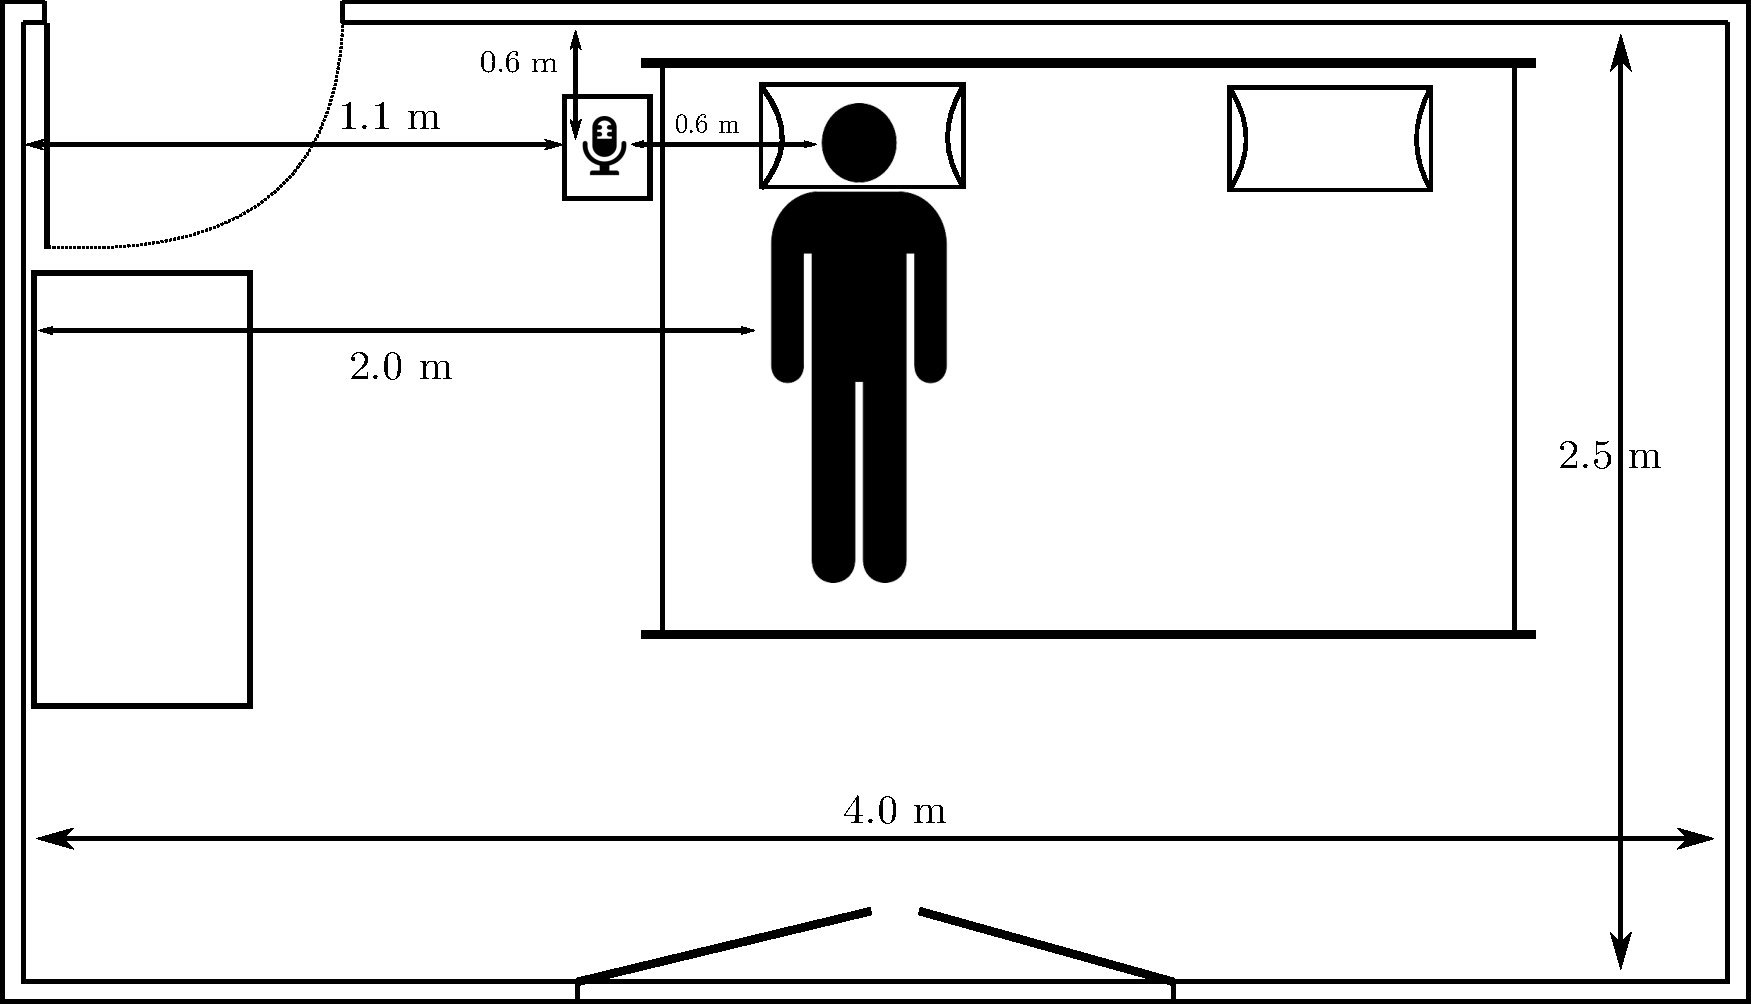
\includegraphics[width=0.8\columnwidth]{img/room.pdf}
	\caption{Plant of the recording room.} 
	\label{fig:room}
\end{figure}


\subsubsection{Dataset splitting:}
The original recordings have been manually labelled, annotating the snore events onset and offset with a resolution of 1 second. The audio sequences have been divided into chunks of 10 minutes, and only those with the highest number of snore events have been used in the experiments. 
The dataset is organized into subjects, which can be respectively used as \emph{training} or \emph{validation} sets in a two fold cross validation strategy (i.e., Leave One Subject Out procedure). The number of events per class in the database is strongly unbalanced as reported in \tableref{a3snore}. Thus, the snore detection task is challenging, due to the high number of noises on the A3-SNORE dataset. 

\begin{table}[ht]
	\centering
	\caption[A3-SNORE dataset]{Difference of recording times for each class, divided by snorers.}
	\begin{tabular}{cccccc}
		\hline
		\multicolumn{6}{c}{\textbf{A3-SNORE dataset}} \\
		\hline
		\# & Gender & Age & Snoring (SN) & Total Duration (Tot) & Ratio (SN/Tot) \\
		\hline
		Snorer 1 & M & 48 & 33m-27s & 3h-12m-0s & 14.5\% \\
		Snorer 2 & M & 55 & 21m-21s & 3h-50m-0s & 11.1\% \\
		\hline
		\multicolumn{3}{l}{Total} &	54m-48s	& 7h-02m-0s	& 12.8\%\\
		\hline    
	\end{tabular}	
	\label{a3snore} 
\end{table}

\subsection{Acoustic Novelty Detection}

\label{sec:databases}
This section describes the three databases evaluated in our experiments: A3Novelty, PASCAL CHiME, and PROMETHEUS.

\subsubsection{A3NOVELTY}

%FABIO Description of A3Corpus taken from ESWA paper. Io l'ho parafrasata in modo "light"...vedete voi se bisogna modificarla di più.

%TODO: add description of the database.

%TODO: add final table including stats on the datasets (number of abnormal sounds, duration etc...


The A3Novelty corpus\footnote{\label{note:a3}\url{http://www.a3lab.dii.univpm.it/research/a3novelty}} includes around 56 hours of recording acquired in a laboratory of the Università Politecnica delle Marche. 
These recordings were performed during different day and night hours, so very different acoustic conditions are available.
A variety of \emph{novel} events were randomly played back by a speaker (e.g., scream, fall, alarm or breakage of objects) during the recordings.

Eight microphones were used in the recording room for the acquisitions: four Behringer B-5 microphones with cardioid pattern and an
array of four AKG C400 BL microphones spaced by 4\,cm, then A MOTU 8pre sound card and the NU-Tech software were utilised 
to record the microphone signals. The sampling rate was equal to 48\,kHz.


The abnormal event sounds (cf.  Table \ref{tab:events}) can be grouped into four categories and they are freely available to download from \url{http://www.freesound.org}:
\begin{itemize}
	\item \textit{Sirens}, three different types of sirens or alarm sounds.
	\item \textit{Falls}, two occurrences of a person or an object falling to the ground.
	\item \textit{Breakage of objects}, noise produced by the breakage of an object after the impact with the ground.
	\item \textit{Screams}, four different human screams, both produced by a single person or by a group of people.
\end{itemize}


The A3Novelty corpus is composed of two types of recordings:
\emph{background}, which contains only background sounds such as human speech, technical tools noise and environmental sounds and \emph{background with novelty}, which contains in addition to the background the artificially generated novelty events.

In the original A3Novelty database the recordings are segmented in sequences of 30 seconds. In order to limit the size of training data, we randomly selected 300 sequences from the \emph{background} partition to compose of training material (150 minutes), and 180 sequences from the \emph{background with novelty} partition to compose the testing set (90 minutes). The test set contains 13 novelty occurrences.

For reproducibility, the list of randomly selected recordings, as well as the train and test set are made available % \footnotemark[\ref{note:a3}]. %ndFAB\footnotemark [3].


%\begin{table}[t]
%\centering
%\begin{tabular}{lccc}
%\hline
%\textbf{Rec Type} & \textbf{Day/Night} & \textbf{Length (hh:mm)} & \textbf{Novelty events}\\
%\hline
%\multirow{2}{*}{Background} & Day & 12:00 & -\\
%& Night & 24:00 & -\\
%\hline
%Background & Day & 9:00 & 16\\
%with novelty & Night & 12:00 & 30\\
%\hline
%\end{tabular}
%\caption{Recordings details.}
%\label{tab:recs_detail}
%\end{table}


\subsubsection{PASCAL CHiME}
\label{subsec:pascal}

The original dataset is composed of around 7 hours of recordings of a home environment, taken from the PASCAL CHiME speech separation and recognition challenge \cite{barker2013pascal}. 
It consists of a typical in-home scenario (a living room), recorded during different days and times,
while the inhabitants (two adults and two children) perform common actions, such as talking, watching television, playing, or eating. The dataset was recorded in stereo (with a binaural microphone) and a sample-rate of 16\,kHz. In the original PASCAL CHiME database the recordings are segmented in sequences of 5 minutes duration. In order to limit the size of training data, we randomly selected sequences to compose 100 minutes of background for the training set, and around 70 minutes for the testing set. For reproducibility, the list of randomly selected recordings, as well as the train and test set are made available\footnote{\url{http://a3lab.dii.univpm.it/webdav/audio/Novelty_Detection_Dataset.tar.gz}}. 
%The test set was generated adding different kinds of sounds\footnote{taken from www.freesound.org}, such as screams, alarms, falls and fractures (cf.\ Table \ref{tab:events}). 
%The test set did not include any overlapping events, the events were  and they were added at random position thus the distance between one event and another is not fixed. %ndFAB\footnotemark [1].
% %VES
The test set was generated adding different typologies of sounds\footnote{taken from www.freesound.org}, such as screams, alarms, falls and fractures (cf.\ Table \ref{tab:events}), after their normalization to the volume of the background recordings. % %
The events in the test set were added at random position (avoiding overlapping), thus the distance between one event and another is not fixed. %ndFAB\footnotemark [1].




\subsubsection{PROMETHEUS}
\begin{table}[t]
	\centering
	\tabcolsep=0.10cm
	\renewcommand{\arraystretch}{1.0}
	\caption[Acoustic novel events]{Acoustic novel events in the test set. Shown are the number of different events per database, the average duration, and the total duration in seconds per event type. The last column indicates the total number of events and total duration across the databases. The last line indicates the total duration in seconds of the test set including normal and novel events per database.}
	
	\begin{tabular}{ l || c c || c c || c c | c c | c c | c c || c c }
		\textbf{Events} & \multicolumn{2}{|c||}{A3Novelty} & \multicolumn{2}{|c||}{PASCAL CHiME} & \multicolumn{8}{|c||}{PROMETHEUS} & \multicolumn{2}{|c}{Total}\\
		\textbf{} & \multicolumn{2}{|c||}{} & \multicolumn{2}{|c||}{} & \multicolumn{2}{|c|}{ATM} & \multicolumn{2}{|c|}{Corridor} & \multicolumn{2}{|c|}{Outdoor} & \multicolumn{2}{|c||}{Smart-room} & \multicolumn{2}{|c}{}\\
		\textbf{} & \# & time(avg.) & \# & time(avg.) & \# & time(avg.) & \# & time(avg.) & \# & time(avg.) & \# & time(avg.) & \# & time\\
		\hline
		Alarm			& - & -		& 76 & 435.8 (6.0) 	 				& - & -			& 6 & 84.0 (14.0)	& - & -				& 3 & 9.0 (3.0)		& 85 & 528.8\\
		Anger			& - & - 				& - & - 				& - & -			& - & -				& 6 & 293.0 (48.8)		& - & - 			& 6 & 293.0\\  
		Fall 			& 3 & 4.2 (2.1)		& 48 & 89.5 (1.8) 	& - & -	 		& 3 & 3.0 (1.0)		& - & -				& 2 & 2.0 (1.0) 		& 55 & 98.7\\
		Fracture		& 1 & 2.2 			& 32 & 70.4 (2.2) 	& - & - 			& - & -				& - & -				& - & - 				& 33 & 72.6\\
		Pain			& - & -			 	& - & - 			& - & -	 		& 2 & 8.0 (4.0)		& - & -				& 5 & 67.0 (13.4) 		& 7 & 75.0\\
		Scream			& 6 & 10.4(1.7)		& 111 & 214.6 (1.9) 	& 5 & 30.0 (6.0)	& 25 & 228.0 (9.1)	& 4 & 48.0 (12.0)		& 10 & 234.0 (23.4) & 159 & 762.2\\
		Siren			& 3 & 20.4 (6.8)		& - & - 				& - & - 			& - & -				& - & -				& - & -				& 3 & 18.1\\
		\hline
		Total			& 13 & 38.1 (2.9) & 267 & 810.3 (3.1) 	& 5 & 30.0 (5.0) 		& 36 & 323.0 (9.0) 	& 10 & 341.0 (34.1) 	& 20 & 312.0 (15.6) & 348 & 1848.4\\
		\hline\hline
		Test time & - & 5400.0 				& - & 4188.0 	& - & 750.0			& - & 960.0	& - & 1620.0				& - & 1020.0		& - & 13938.0\\
		
	\end{tabular}
	\label{tab:events}
\end{table}

The PROMETHEUS database \cite{ntalampiras:probabilistic} contains recordings of various scenarios designed to serve a wide range of real-world applications. The database includes: 1) a \textit{smart-room} indoor home environment including phases where a user is interacting with an automated speech-driven home assistant, 2) an outdoor public space consisting of \textit{a}) interaction of people with an \textit{ATM}, \textit{b}) an \textit{outdoor} security scenario in which people are waiting in front of a counter, and 3) an  indoor office \textit{corridor} scenario for security monitoring in standard indoor space. 
%The first one is intended to be representative of particular activities which take place inside an intelligent environment, including phases where the user is interacting with an automated speech-driven home assistant. As for the second setting, two scenarios with different scopes were captured: 1) ATM scenario, which included interactions of people with an ATM, and 2) security scenario, in which people in a queue are waiting for service in front of a counter and can be utilized as a general-purpose scenario with many applications (e.g., bank, airport, etc.). The third setting was used for security scenarios in a standard indoors space. 
These scenarios substantially differ in terms of acoustic environment. The indoor scenarios were recorded under quiet acoustic conditions, whereas the outdoor recordings were conducted in an open-air public area and contain non-stationary background noise.   
The smart-home scenario contains recordings of five professional actors performing five single-person and 14 multiple-person action scripts. The main activities include human-machine interaction with a virtual home agent, a number of alternating normal and abnormal activities specifically designed to monitor and interpret human behaviour. The single-person and multiple-person actions include abnormal events, such as: falls, alarm followed by panic, atypical vocalic reactions (pain, fear, anger), or fractures. Examples are: walking to the couch, sitting or interacting with the smart environment to turn the TV on, open the windows, or decrease the temperature. The scenarios were recorded three to five times, by changing the actors and their roles in the action scripts.
Table \ref{tab:events} provides details on the number of abnormal events per scenario, including average time duration.


\section{The DIRHA Dataset}
\label{sec:dataset}

\begin{figure}[h]
	\centering
	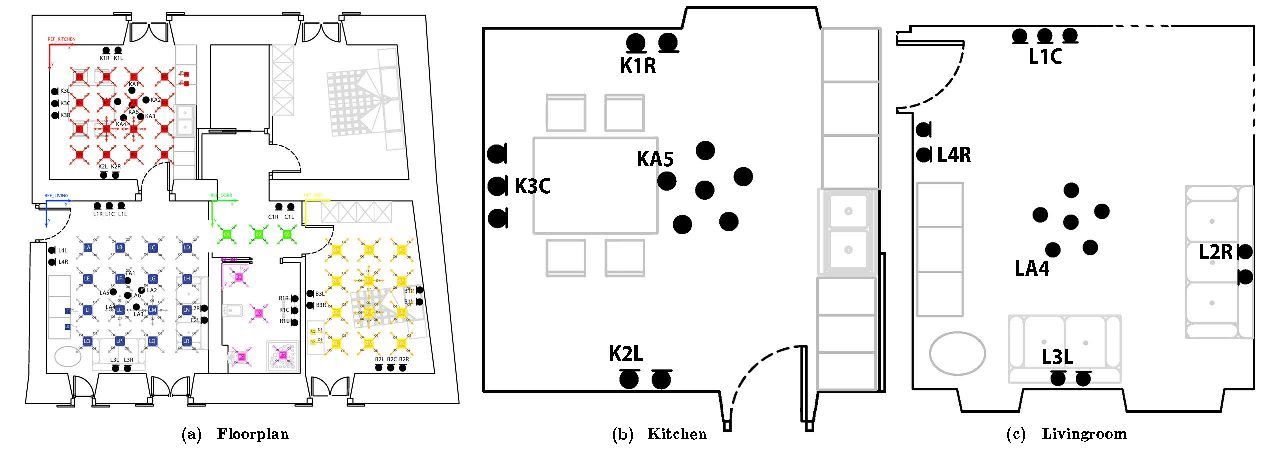
\includegraphics[width=\textwidth]{img/plan}
	\caption{The map of the apartment used for the DIRHA project (a). Figures (b) and (c) show the considered rooms, with the disposition of their relative microphones. }
	\label{fig:DIRHA_map}
\end{figure}

The analysis of the DNN-SLOC performance has been conducted on the DIRHA dataset \cite{cristoforetti2014dirha}, characterized by diverse scenes, rooms, microphones and noise conditions\footnote{\url{http://dirha.fbk.eu/simcorpora}}. In details, the apartment where the dataset has been recorded consists in five rooms and a total of 40 microphones. These are arranged in linear and circular arrays, with the first ones placed on the walls of all rooms, and the circular ones are placed on the ceiling of the living room and of the kitchen (\figref{fig:DIRHA_map}).

The dataset is composed of two subsets, named \emph{Simulated} and \emph{Real}. For each of them several \textit{scenes} have been recorded, composed of typical situations observable in a domestic context. As reported in \tableref{tab:dataset}, the two subsets differ in terms of scenes and total length: in the Simulated set the scenes length is fixed to 60 seconds, while it varies in the Real set. In addition, the latter has been recorded with persons moving in the rooms and speaking towards different directions throughout the scenes, whilst the Simulated has been obtained by convolving a fixed set of measured Room Impulse Responses (RIRs) with recorded signals.
The Simulated subset is also characterized by a lower SNR compared to the Real one and overlapping speech does not occur.

Our study focuses on two rooms of the dataset, i.e.,  the Kitchen and the Living Room, due to three main aspects. First of all, these rooms consist in the area of a home-environment where most of the events take place. In addition, being the widest rooms of the apartment, the localization task is more challenging. \textcolor{red}{The room dimensions are respectively $4.79$\,m~$\times$~$3.80$\,m for the Kitchen and $4.79$\,m~$\times$~$4.85$\,m for the Living Room.}
Finally, the number of microphones are higher compared to the other rooms, and they comprise both wall and ceiling arrays.

\begin{table}[t]
	%\renewcommand{\arraystretch}{1.2}
	\centering
	%	\small
	\caption{Main differences between the Real and Simulated subsets.}
	\resizebox{.75\columnwidth}{!}{%
		\begin{tabular}{c|c|c}\hline
			& \textbf{Real} & \textbf{Simulated} \\ \hline
			\textbf{Nr.\ of Scenes}  & 22 & 80 \\ \hline
			
			\textbf{Total Duration} &  21.5 min. & 80 min.  \\  \hline
			\multirow{2}{*}{\textbf{Speech Percentage}}	&  12.9\%  & 23.6\%  \\
			& 	2.8  min.	& 18.9 min. \\ \hline
			\textbf{Source} & human (moving) & loudspeaker (static) \\ \hline
			\textbf{Background} & quiet & various \\ \hline
			\textbf{Noise Source Rate} & low & high \\ \hline
			\textbf{Overlapping Events} & no & yes \\ \hline  
		\end{tabular} 
	}
	\label{tab:dataset}
\end{table}

\section{Datasets for Sound Event Classification}

\subsection{Acoustic Road Roughness Classification}
The dataset built for this work is done with a multi-channel microphone arrangement, with the prospect of conducting different assessments at once or to exploit microphone diversity to improve the classification. More specifically, two microphones have been placed close to the rear wheels, one in front of the front left wheel, one inside the engine compartment and two inside the cockpit, close to the driver head and close to the right passenger head. The rear wheel microphones have been placed off-axis, in order to avoid dirt from the wheel and protected by the wheelhouse to reduce the effect of wind. Figure \ref{fig:car-mic} shows the positioning of all microphones. External microphones are \textit{PCB Piezotronics} model 130A24. These are IP55 microphones and they have been protected with a melamine resin foam for sound absorption to reduce the effect of wind. The internal microphones are \textit{PCB Piezotronics} model 378C20. The front-right wheel has been excluded from recordings after first informal evaluations because it picked a large amount of engine noise with respect to the other microphones. The rear-right microphone, vice versa, was found to be the best choice because the noise from the engine was the lowest and it has been used for this first evaluation. The engine compartment microphone has been used to record the engine conditions for future use. In \figref{fig:car-rr-and-fl} are shown the images of the microphones installation. 

\begin{figure}[ht]
	\centering
	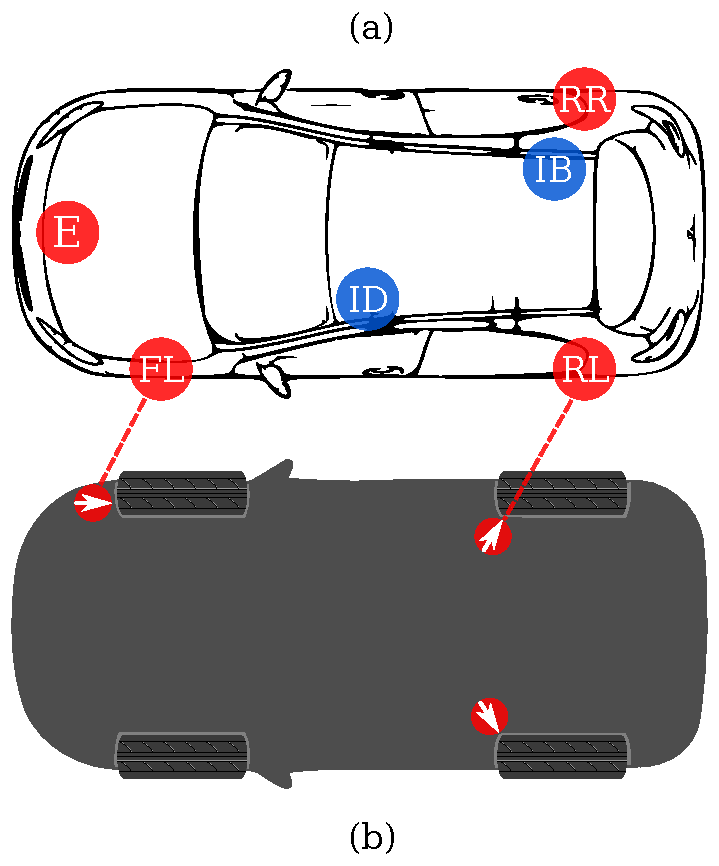
\includegraphics[width=0.5\textwidth]{img/car-mic}
	\caption[Position of the microphones in the car used to record the dataset]{Positioning of the microphones in the car used to record the dataset, top view (a) and bottom view (b). The microphones are placed in the engine compartment (E), close to the front-left, rear-left and rear-right tyres (FL, RL, RR), and inside the car close to the driver or in the back seat (ID, IB). The last two microphones are \textit{PCB Piezotronics} model 378C20 type microphones, while all the others are IP55 \textit{PCB Piezotronics} model 130A24 microphones. The microphones are omnidirectional, however the arrows in (b) show how the capsule was positioned to minimize wind effect. The rear microphones are protected in the wheelhouse.}
	\label{fig:car-mic}
\end{figure}

\begin{figure}[t]
	\centering
	\begin{subfigure}[b]{0.48\textwidth}
		\includegraphics[width=\textwidth]{img/Rear-Right.jpg}
		\subcaption{Rear right tyre microphone.}
	\end{subfigure}
	\hfil
	\begin{subfigure}[b]{0.48\textwidth}
		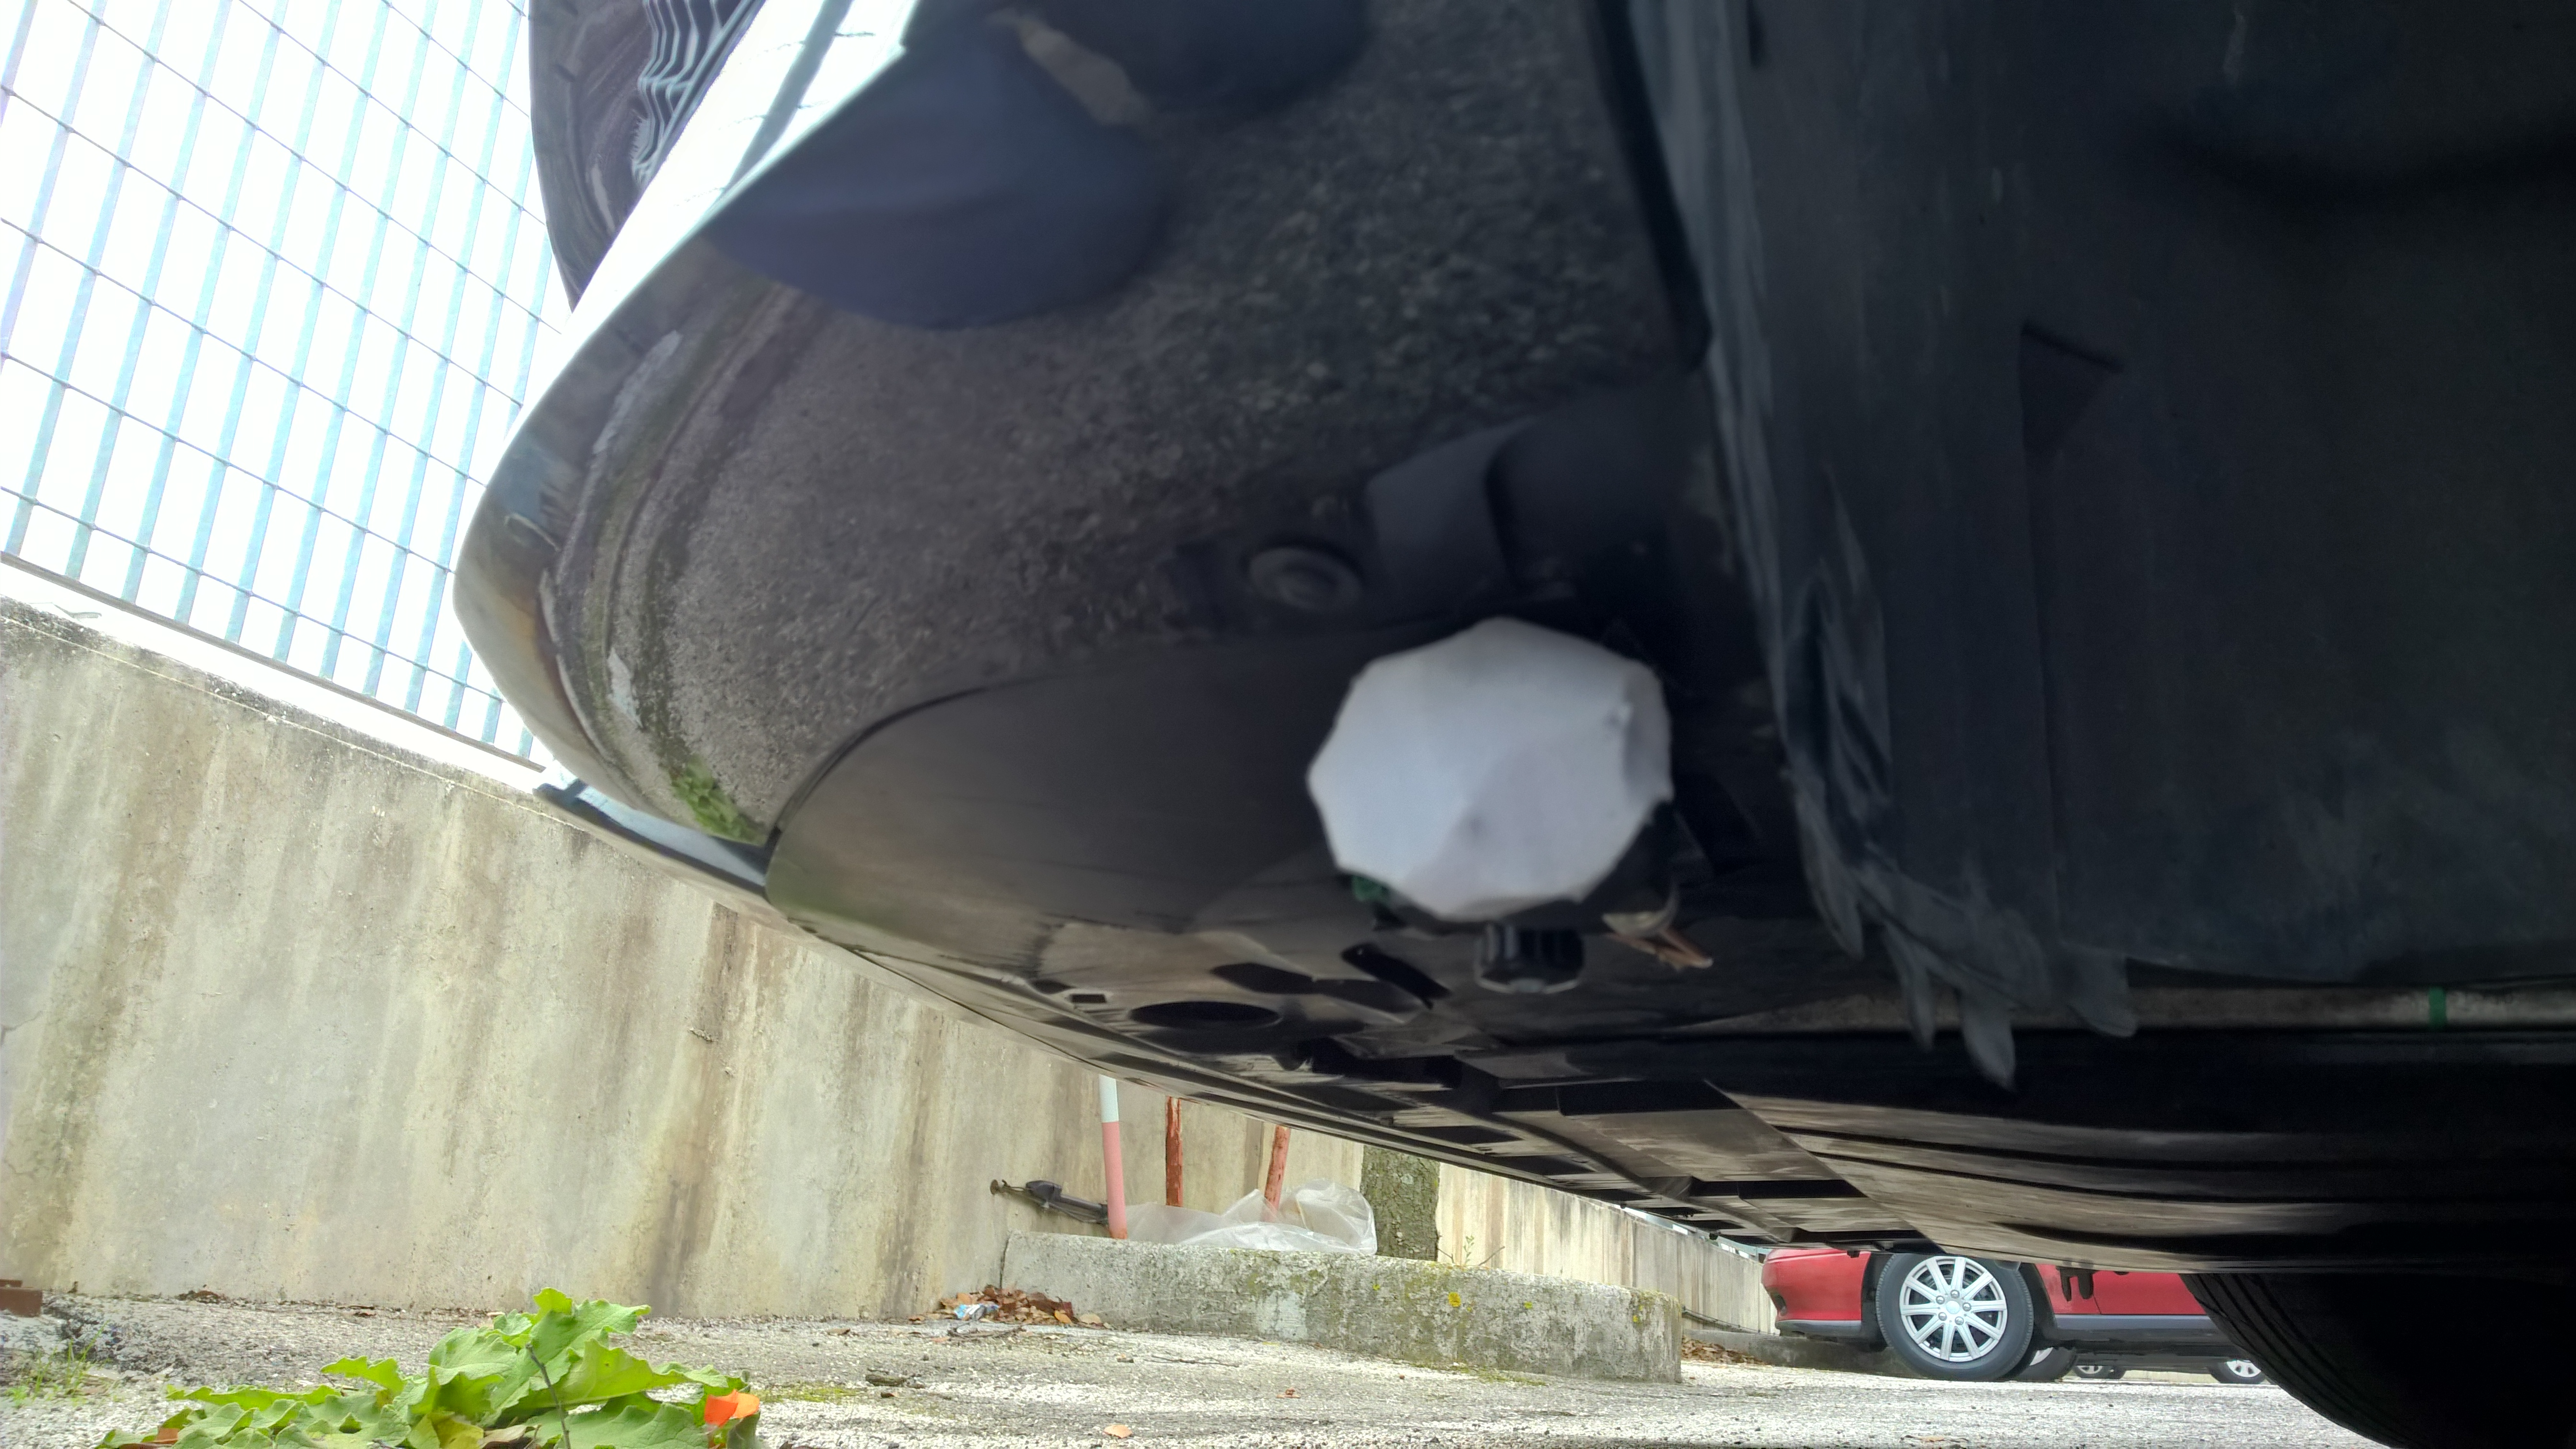
\includegraphics[width=\textwidth]{img/Front-Left.jpg}
		\subcaption{Front left tyre microphone.}
	\end{subfigure}
	
	
	\caption[\textit{PCB Piezotronics} model 130A24 microphones]{Pictures of the \textit{PCB Piezotronics} model 130A24 microphones positioned near the rear right and front left tyres, according to "RR" and "FL" red circles in \figref{fig:car-mic}. The microphones are enclosed by a melamine resin foam with open cell network structure to reduce the wind noise.}
	\label{fig:car-rr-and-fl}
\end{figure}



The car employed to build the dataset is Mercedes A Class from 2014. In addition to the audio signals, the GPS signal has been recorded to track down the car speed and position at any given time. A mobile multi-channel front end, \textit{HEAD Acoustics SQuadriga II}, has been employed as acquisition device, being able to monitor and record 8 contemporary channels at different sample rates, and to store GPS antenna and CAN bus signals.
All audio signals are sampled at 44100\,Hz, 24-bits. The external microphones used -26 dBV as input range while the interior microphones had -16 dBV as input range.
To facilitate the labelling operations, a camcorder \textit{BC Master DC10}\footnote{\url{http://www.bc-master.com/product/car-dash-camera-dc10}} was installed on the dashboard of the car. In addition to the video, it provides the speed information obtained through its own GPS antenna and it records the cockpit audio, useful for taking vocal notes while driving.

The data recorded with the \textit{HEAD Acoustics SQuadriga II} have been exported by means of the software \textit{HEAD Acoustics ArtemiS SUITE} in the uncompressed WAV audio format with a 32-bit float representation.

All recordings were taken in dry conditions in the urban and suburban areas of Ancona (Italy) with variable speed, traffic conditions and pavement roughness. Only roads that had been recently asphalted were considered and multiple takes at different speed for each road have been performed. The dataset is not perfectly balanced and is characterized by 41\% of rough road samples and 59\% of smooth road samples. For this reason a balanced version of the dataset, i.e. with equal number of smooth and rough samples, has been created by pruning excess samples for the most populated class. 
The result of the recording sessions is a 50-minutes-long dataset (41 minutes for the balanced version), with 6 audio channels and a speed channel. Labels for the roads have been annotated manually.

The spectrograms from two audio samples belonging to the smooth and rough classes are shown in Figure \ref{fig:spectrograms_road}.

\begin{figure}[ht]
	\centering
	\begin{subfigure}[b]{0.48\textwidth}
		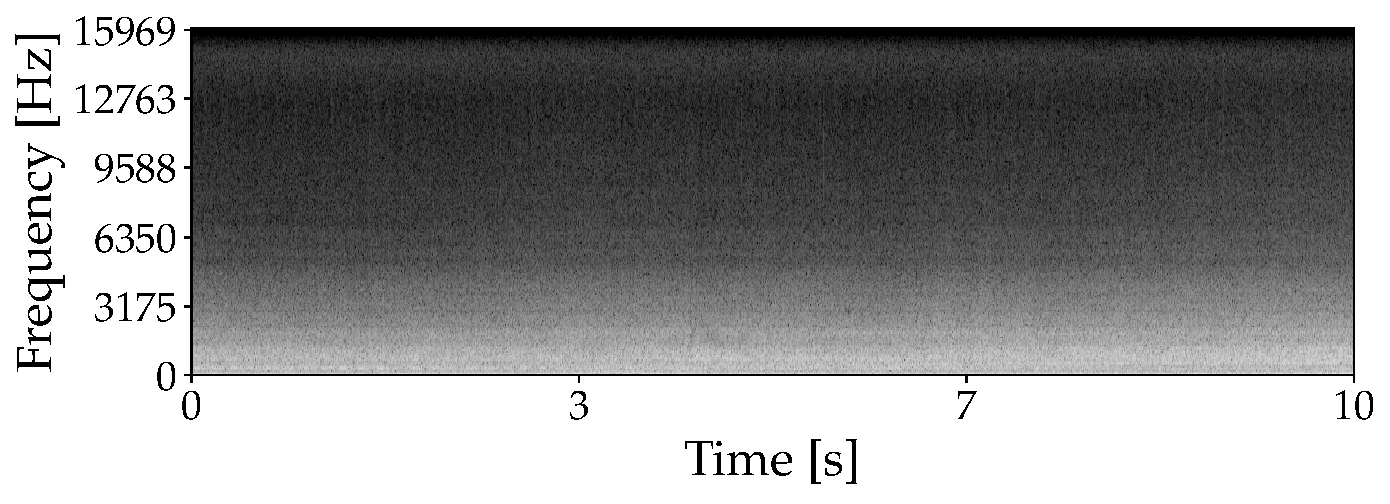
\includegraphics[width=\textwidth]{img/specgram_REC007}
		\subcaption{Smooth road.}
	\end{subfigure}
	\hfil
	\begin{subfigure}[b]{0.48\textwidth}
		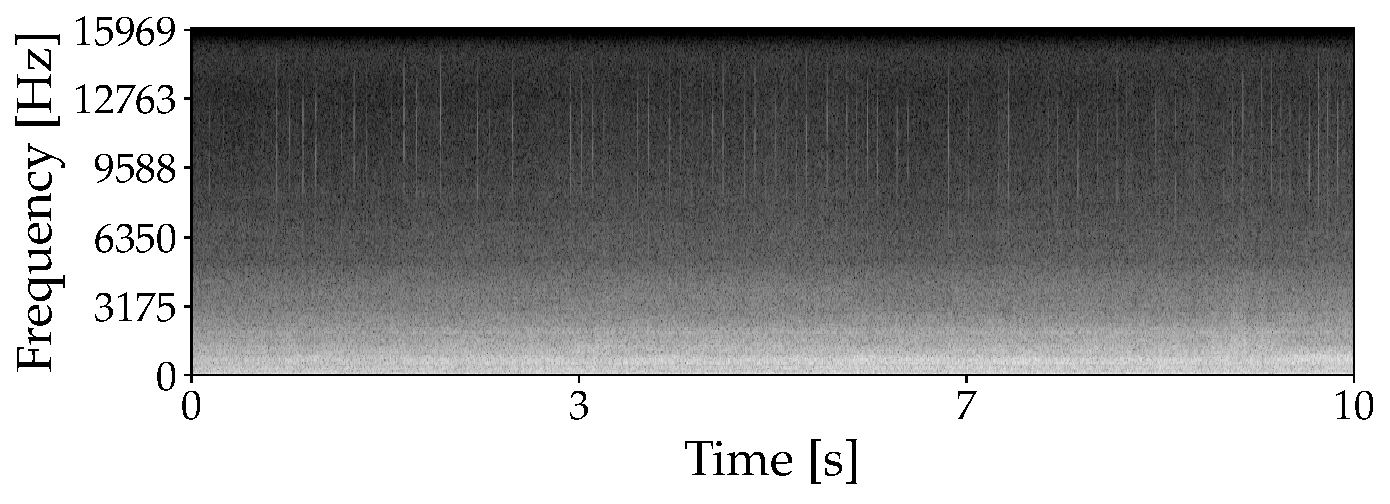
\includegraphics[width=\textwidth]{img/specgram_REC015}
		\subcaption{Rough road.}
	\end{subfigure}
	
	
	\caption[Spectrograms from 10 second samples]{Spectrograms from 10 second samples of (a) smooth urban road, (b) rough highway asphalt.}
	\label{fig:spectrograms_road}
\end{figure}

\subsection{Classification of Snore Sounds Excitation Locations}

\section{The MPSSC dataset}
\label{section:dataset}
The MPSSC dataset is composed of more than 30 hours of audio recordings captured during DISE examinations of 224 subjects from three medical centers recorded between 2006 and 2015. Recording equipment, microphone type, and location differ among the medical centers, so do the background noise characteristics. From the original signals (raw PCM, sample rate 16\,000\,Hz, quantization 16 bit) 843 early identifiable, single site of vibration snore events have been extracted and manually screened from medical experts.
Following the 4-class VOTE scheme, each sound file in the dataset is labelled as V, O, T, E, depending on the tissue from which snore sound originates, as shown in \figref{fig:vote}. They are respectively:
\begin{itemize}
	\item (V) - Velum (palate), including soft palate, uvula, lateral
	velopharyngeal walls;
	\item (O) - Oropharyngeal lateral walls, including palatine tonsils;
	\item (T) - Tongue, including tongue base and airway posterior to the tongue base;
	\item (E) - Epiglottis.
\end{itemize}

\begin{figure}[t]
	\centering
	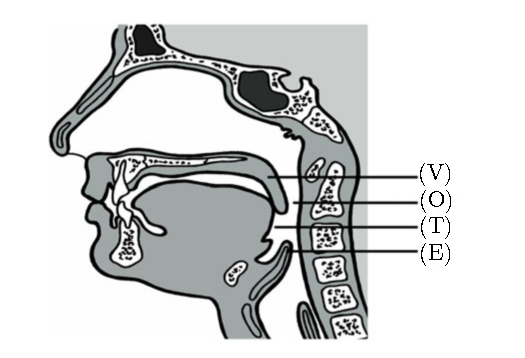
\includegraphics[width=0.6\linewidth]{img/vote.pdf}
	\caption[VOTE positions]{Corresponding positions of the VOTE classification in the upper airway. Picture courtesy of \cite{janott2014akustical}.} 
	\label{fig:vote}
\end{figure}


The dataset is divided into three subsets: \textit{train}, \textit{devel} and \textit{test}.
The number of events per class in the database is strongly unbalanced with a high preeminence of the ``Velum'' (V)-class  and ``Oropharyngeal'' (O)-class (85\% of samples) but in line with the likelihood of occurrence during normal sleep, while 10\% and 5\% of samples respectively belongs to E-events and T-snores. Details of class occurrences are shown in Table I.

\begin{table}[t]
	\centering
	\begin{tabular}{cccc}
		\toprule
		\multicolumn{4}{c}{\textbf{The Munich-Passau Snore Sound Corpus}} \\
		\midrule
		\#  \rule{10pt}{0pt}	& train  \rule{10pt}{0pt} & devel & test\\
		\midrule
		V \rule{10pt}{0pt}	& 168  \rule{15pt}{0pt} & 161 & 155\\
		O \rule{10pt}{0pt}	& 76  \rule{15pt}{0pt} & 75 & 65\\
		T \rule{10pt}{0pt}	& 8  \rule{15pt}{0pt} & 15 & 16\\
		E \rule{10pt}{0pt}	& 30  \rule{15pt}{0pt}& 32 & 27\\
		\bottomrule
		$\Sigma$  \rule{10pt}{0pt} & 282  \rule{13pt}{0pt} & 283 & 263\\
	\end{tabular}
	\caption[The Munich-Passau Snore Sound Corpus]{The Munich-Passau Snore Sound Corpus - The table shows the number of events per class in train, devel and test.}
	\label{tab:mpssc} 
\end{table}

%\begin{figure*}[t]
%	\centering
%	\includegraphics[width=\linewidth]{imgs/spectr-vote.png}
%	\caption{Waveforms and spectrograms of VOTE events}{(a) V (velum); (b) O (oropharyngeal); (c) T (tongue base); (d) E (epiglottis). \textbf{Rifare in HD, eventualmente aggiungere SCAT plot}} 
%	\label{fig:spectrograms}
%\end{figure*}


\begin{figure*}[t]
	\centering
	\begin{subfigure}{.40\textwidth}		
		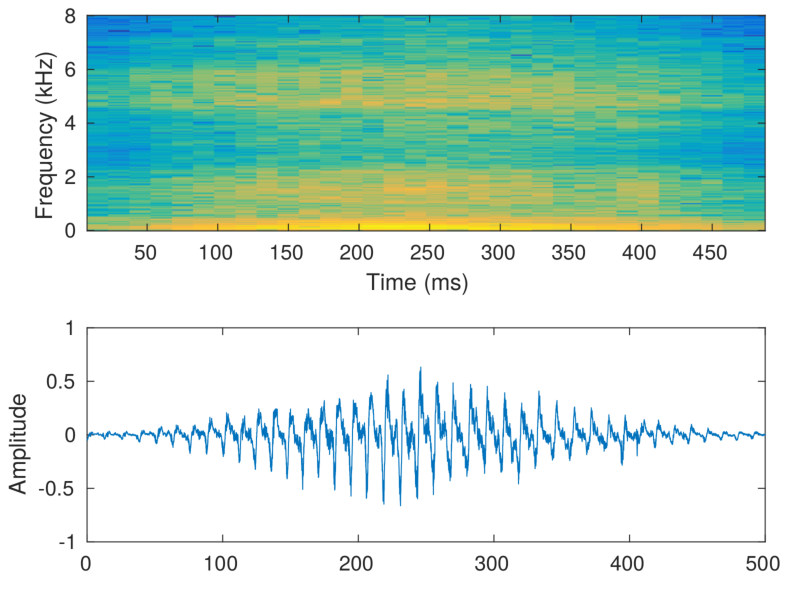
\includegraphics[width=0.9\linewidth]{img/V_spec_crop.pdf}
		\caption{}
		\label{fig:V}
	\end{subfigure}
	\begin{subfigure}{.4\textwidth}
		%\centering
		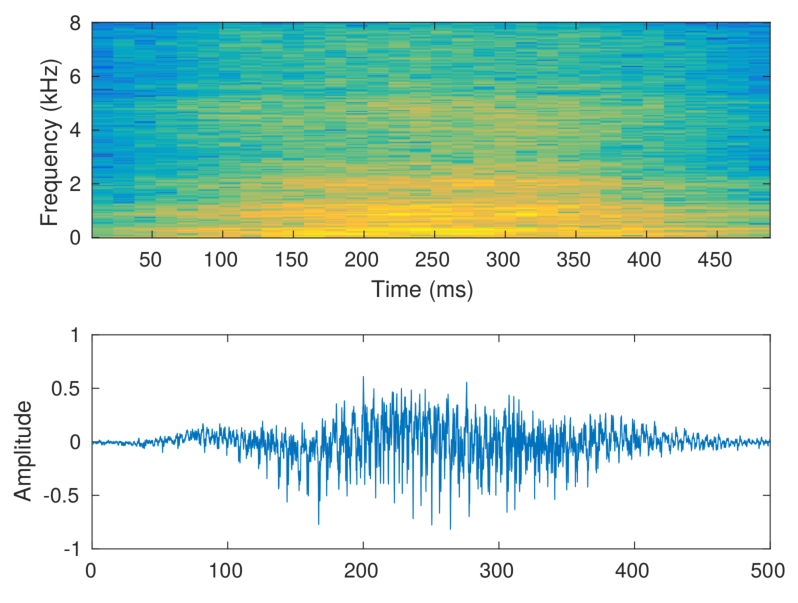
\includegraphics[width=0.9\linewidth]{img/O_spec_crop.pdf}
		\caption{}
		\label{fig:O}
	\end{subfigure}
	\begin{subfigure}{.40\textwidth}
		%\centering
		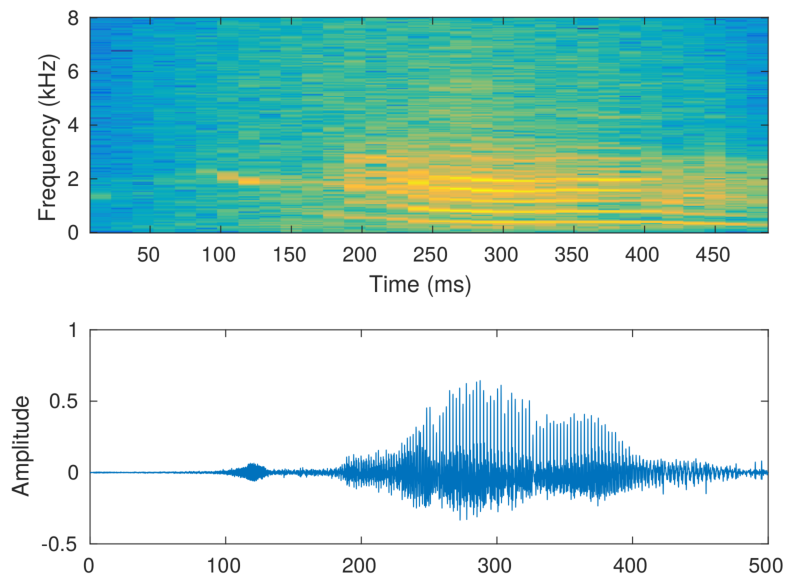
\includegraphics[width=0.9\linewidth]{img/T_spec_crop.pdf}
		\caption{}
		\label{fig:T}
	\end{subfigure}
	\begin{subfigure}{.40\textwidth}
		%\centering
		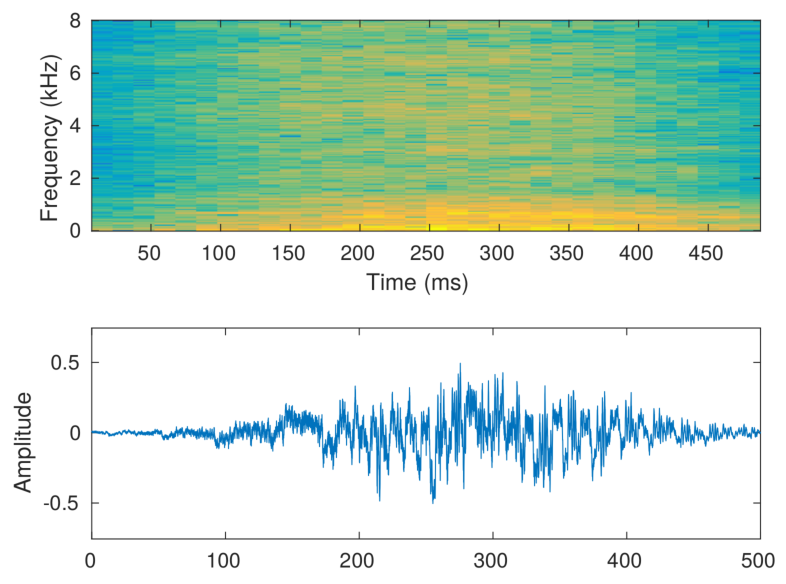
\includegraphics[width=0.9\linewidth]{img/E_spec_crop.pdf}
		\caption{}
		\label{fig:E}
	\end{subfigure}
	\caption{Waveforms and spectrograms of VOTE events}{(a) V (velum); (b) O (oropharyngeal); (c) T (tongue base); (d) E (epiglottis).}
	%\caption{Scat spectrum of VOTE events.  The top image is made of first-order coefficients, organized in a time-scale matrix. at the bottom of the image appear very low frequencies. The second-order coefficients for a fixed scale $m_1$, are shown in the bottom image, again in a time-scale matrix.}{(a) V (velum); (b) O (oropharyngeal); (c) T (tongue base); (d) E (epiglottis).}
	\label{fig:spectrograms}
\end{figure*}
As shown in the waveforms and the related spectrograms in \figref{fig:spectrograms}, the main energy components in three of the classes are concentrated in the frequency area below around 2000 Hz. Energy and spectral distribution characteristics are similar, except for the Type T, which shows higher energy content above 2500 Hz compared to the other three.


\subsection{Bird Audio Detection}
%\label{ssec:dataset}
According to the DCASE 2018 guidelines, the performance of the proposed algorithm has been assessed firstly by using the development dataset for training and validation of the system. Then, a blind test on the provided evaluation dataset was performed with the models which achieved the highest performance and submitted to the organizers of the challenge. The complete dataset is composed of recordings belonging to five different collections. Further details are reported below: %Further details are reported in Table \ref{tab:dataset}.

\begin{itemize}
	\item ``freefield1010'': a collection of 7690 excerpts from field recordings around the world;
	\item ``warblrb10k'': a crowsourced dataset recorded with the \textit{Warblr}\footnote{https://www.warblr.co.uk/} smartphone app. It covers a wide distribution of UK locations and environments and includes weather noise, traffic noise, human speech and even human bird imitations; 8000 samples are used in the development dataset while a held-out set of 2,000 recordings from the same conditions is included in the evaluation split;
	\item ``BirdVox-DCASE-20k'': 20000 files containing remote monitoring flight calls collected from  recordings units placed near Ithaca, NY, USA during the autumn of 2015;
	\item ``Chernobyl'': dataset collected from unattended remote monitoring equipment in the Chernobyl Exclusion Zone (CEZ). A totoal of 6620 audio files cover a range of birds and includes weather, large mammal and insect noise sampled across various CEZ environments, including abandoned village, grassland and forest areas;
	\item ``PolandNFC'': 4000 recordings obtained from a project of monitoring of autumn nocturnal bird migration. They were collected every night, from September to November 2016 on the Baltic Sea coast, Poland, using Song Meter SM2 units with microphones mounted on 3–5 m poles.
\end{itemize}

\begin{table}[t]
	\centering
	\begin{tabular}{|c|c|c|}
		\hline
		\ \textbf{Collection} \rule{0pt}{10pt} & \textbf{N. of samples}  & \textbf{Balance} \\
		\hline
		\hline	
		\multicolumn{3}{|c|}{\textbf{Development Dataset}  \rule{0pt}{10pt}} \\ 
		\hline
		``warblrb10k'' & 8000 & 0.75 \\
		\hline
		``BirdVox-DCASE-20k'' & 20000 & 0.5 \\
		\hline
		``freefield1010'' & 7690 & 0.25 \\
		\hline
		
		Total 	& 35690	& 0.5 \\
		
		\hline
		\hline
		
		\multicolumn{3}{|c|}{\textbf{Evaluation Dataset}  \rule{0pt}{10pt}} \\ 
		\hline
		``warblrb10k\_test'' & 2000 & - \\
		\hline
		``Chernobyl'' & 6620 & - \\
		\hline
		``PolandNFC'' & 4000 & - \\
		\hline
		Total 	& 12620 & - \\
		\hline
	\end{tabular}
	\caption{Details of the dataset we used for the algorithm development. The table shows the number of audio files and the ratio between positive/negative samples (if available) of each used data collection.}
	\label{tab:dataset} 
\end{table}

The organizers recommended a 3-way cross-validation (CV) for the algorithms development, thus in each fold we used two sets for training and the other one as validation set in order to have scores comparable with the others challenge participant.

\section{Evaluation Metrics}
\label{sec:evaluation_metrics}
Evaluation is usually referred as estimating the performance of a system under test
when confronted with new data. For an objective evaluation, the system is fed
previously unseen data for which reference annotations are available. The system output is then compared to the reference to calculate measures of its performance.

What performance means and how it should be measured may vary depending
on the specifications and requirements of the developed system: We can measure
accuracy to reflect how often the system correctly classifies or detects a sound, or we can measure error rates to reflect how often the system makes mistakes. By using
the same data and the same methodology to evaluate different systems, a fair and direct comparison can be made of systems’ capabilities.

The metrics used in detection and classification of sound events include accuracy, precision, recall, F-scor, area under the curve (AUC) or error rate (ER). There is no metric universally good for every kind of algorithm, as they each reflect different perspectives on the ability of the system.

\subsection{Metrics Computation}
Basically, the evaluation metrics are computed by comparing the prediction of the system under analysis with the respective annotations or \textit{ground truth}. Thus, the metrics are calculated based on counts of the correct predictions and different types of errors made by the system.
These counts are referred to as intermediate statistics and are defined depending on the evaluation procedure. These intermediate statistics are defined as follows for a target sound event:

\begin{itemize}
	\item True positive: A correct prediction, meaning that the system output and the reference both indicate the event present.
	\item True negative: The system output and the reference both indicate event not present.
	\item False positive: The system output indicates event  present or active, while the reference indicates event not present.
	\item False negative: The system output indicates event not present or inactive, while the reference indicatesit as present.
\end{itemize}

Sound event classification is usually a single-label multiclass problem, and the resulting intermediate metrics reflect whether the single true class is correctly recognized for each example. In this task there is no distinction between false positives and false negatives. 
In sound event detection, the choice of measurement determines the interpretation of the result: With a segment-based metric, the performance shows how well the system correctly detects the temporal regions where a sound event is
active; with an event-based metric, the performance shows how well the system is able to detect event instances with correct onset and offset. Thus, in the segment-based metric the ground truth and system output are compared in a fixed time grid, and sound events are marked as active or inactive in each segment. For the event-based metric the ground truth and system output are compared at event instance level. Specifically, the intermediate statistics for sound event detection are defined as follows:

\begin{itemize}	
	\item Substitutions $S$: are the number of ground truth events for which we have a false positive and one false negative in the same segment; %, thus: $S(t_1) = \min(FN(t_1),FP(t_1))$;	
	\item Insertions $I$: are events in system output that are not present in the ground truth, thus the false positives which cannot be counted as substitutions;%: $I(t_1) = \max(0,FN(t_1)-FP(t_1))$;
	
	\item Deletions $D$: are events in ground truth that are not correctly detected by the system, thus the false negatives which cannot be counted as substitutions;%: $D(t_1)= \max(0,FP(t_1)-FN(t_1))$.	
\end{itemize}

If we consider the scenario of polyphonic sound event detection, the segment-based metric essentially
splits the duration of the test audio into fixed length segments that have multiple associated labels, reflecting the sound events active anywhere in the given segment. In this respect, evaluation verifies if the system output and reference coincide in the assigned labels, and the length of the segment determines the temporal resolution of the evaluation. 
Event-based metrics compare event instances one to one. Since the time extents of the events detected by the system may not exactly match the ground truth, a common approach is to allow a time misalignment threshold or \textit{time-collar}.

\subsubsection{Performance Metrics}
Measures of performance are calculated based on accumulated values of the intermediate statistics. 
We denote by $TP$, $TN$, $FP$, and $FN$ the sums of the true positives, true negatives, false positives, and false negatives accumulated throughout the test data. In the case of multiclass problem, the accumulation of intermediate statistics can be performed either globally or separately for each class, depending on the nature of the problem (i.e., instance-based or class-based) or datasets characteristics (i.e., highly unbalanced classes).
Based on the total counts of the intermediate statistics, many different measures can be derived.  We can define:

\begin{eqnarray}
\text{Accuracy} =& \frac{TP+TN}{TP+TN+FP+FN} \\
\text{Precision} =& \frac{TP}{TP+FP} \\
\text{Recall} =& \frac{TP}{TP+FN}  \\
\text{F-score} =& \frac{2TP}{2TP+FN+FP}  
\end{eqnarray}

Accuracy measures how often the classifier makes the correct decision,
 as the ratio of correct system outputs to total number of outputs. Precision, recall, and F-score were introduced in the context of information retrieval. F-score can be also calculated as the harmonic mean of Precision and Recall scores:

\begin{equation}
 \text{F-score} = 2 \cdot \frac{\text{Precision}\cdot\text{Recall}}{\text{Precision}+\text{Recall}}
\end{equation}

F-score has the advantage of being a familiar and well understood metric. Its main drawback is that its value is strongly influenced by the choice of averaging and the data balance between classes: in instance-based averaging the performance
on common classes dominates, while in class-based averaging (balanced metrics) it is necessary to at least ensure presence of all classes in all folds in the test data, to avoid cases when recall is undefined.

In the case of sound event detection systems, Error Rate score is the most common evaluation metric. Considering a single time frame  $t_1$, the ER is computed from its intermediate statistics, i.e., the number of substitutions ($S(t_1)$), insertions ($I(t_1)$), deletions ($D(t_1)$) and active sound events from annotations ($N(t_1)$). Formally, for the entire evaluation set:

\begin{equation}
ER = \frac{\sum_{t_1=1}^{T} S(t_1) + \sum_{t_1=1}^{T} I(t_1) + \sum_{t_1=1}^{T} D(t_1)}{\sum_{t_1=1}^{T} N(t_1)},
\end{equation}
where $T$ is the total number of segments $t_1$.


\subsection{Detection Metrics}
Precision and recall rely on hard decisions made for each trial, they typically depend on a threshold applied to some underlying decision variable, i.e., the output of the neural network. 
Lowering the threshold will increase likelihood of accepting both positive and negative examples, improving recall but in many cases hurting precision. Although F-score combines these values at a single threshold in an attempt to balance this
tradeoff, a more complete analysis can be provided by plotting a function proportional to the metric over the full range of possible thresholds. Some examples are, the precision-recall (P-R) curve and the receiver operating characteristic (ROC) curve. The latter plots true positive rate (TPR = $TP/TP+FN$) as a function of the false
positive rate (FPR = 1 - Recall) as the decision threshold is
varied. 

These curves carry rich information, they can be difficult to compare, so a
 single figure of merit summarizing the tradeoff is desirable. The
relative ``compressed'' scores for P-R and ROC curve are respectively Average Precision (AP) score
or Area under curve (AUC), defined as:

\begin{equation}
\text{AP} = \sum_n (R_n-R_{n-1})P_n,
\end{equation}
where $R_n$ and $P_n$ are the Recall and Precision for threshold $n$ respectively and
\begin{equation}
\text{AUC}=\int _{\infty }^{-\infty }{\mbox{TPR}}(T){\mbox{FPR}}'(T)\,dT
\end{equation}
Both AUC and AP vary between 0 and 1, with an uninformative classifier yielding 0.5, while the ideal system yelds 1.


\subsection{Final Remarks}
Estimates of metrics on classes with very few examples are also intrinsically noisy. Any dataset of real-world
recordings will most likely have unbalanced event classes; therefore, the experiment setup must be built with the choice of metric in mind. In a cross-validation approach, a more stable result is given by treating the cross-validation folds as single experiment, meaning that metrics are calculated only after training and testing all folds, not as average of the individual folds nor as average of individual class performance. In addition, reporting the variance among the individual folds’ contributions to the average
can serve as a useful confidence interval.
Anyway, if there are multiple scenes in the dataset, typically evaluation metrics are calculated for each scene separately and then the results are presented as the average across the scenes.


Attention should be also paid to statistical significance of the results and it should be used to calculate the theoretical limits of discriminability of the evaluation, especially when two methods/approaches/techniques are compared.


A detailed and visualized explanation of evaluation score in multi label setting for sound event analysis can be found in  \cite{mesaros2016metrics}.







%In this work we used the Error Rate (ER) as primary evaluation metric to ensure comparability with the reference systems. In particular, for the evaluations on the TUT-SED 2016 and 2017 datasets we consider a segment-based ER with a one-second segment length, while for the TUT-Rare 2017 the evaluation metric is event-based error rate calculated using onset-only condition with a collar of 500 ms. 
%



\graphicspath{{4_sound_event_classification/}}
\chapter{Sound Event Classification}

The task of sound event classification consists of categorize an audio recording into one of a set of predefined categories, by associating a textual descriptor. In this chapter three works belonging to this ``sub-category'' are shown. They are respectively: Snore Sounds Excitation Localization, which has been performed by using \textit{Scattering Transform} and Deep Neural Networks; Road Surface Roughness Classification from Acoustic Signals, which has been performed by means of Convolutional Neural Networks; Bird Audio Detection, which - despite of its name - consists in determining a binary decision for the presence/absence of bird sounds on audio files recorded in very different conditions and it has been performed by using CapsNets.

\section{Snore Sounds Excitation Localization}
\label{sec:snoring_classification}
\begin{figure}[h]
	\centering
	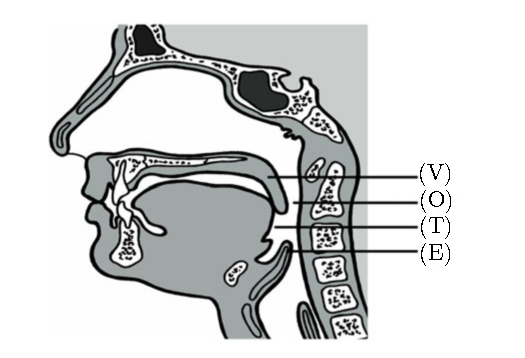
\includegraphics[width=0.6\linewidth]{img/vote.pdf}
	\caption[VOTE locations]{Corresponding positions of the VOTE classification in the upper airway. Picture courtesy of \cite{janott2014akustical}.} 
	\label{fig:vote}
\end{figure}

People spend almost a third of their life sleeping, thus the sleep quality is very important to people's health. Most of us  have experienced trouble sleeping just sometimes, while for some people sleep problems occur regularly; in former cases a sleep disorder is diagnosed. Among these, one of the most common sleep disorder \cite{sleep-disorders} is the chronic snoring.
 
Snoring is defined as the emission, during the sleep, of a sound more or less annoying associated to the respiratory activity. This sound is caused by the vibration of soft tissue in the upper airways. It is confirmed that almost a half of the adult population snores occasionally, while approximately 30\% of the overall population suffers from chronic snoring almost every night \cite{young1997nasal}.
Sound snoring can have a negative impact on normal physical, mental, social and emotional functioning of the person suffering from it and their bed partner \cite{blumen2012snoring}. In addition, it can be associated with Obstructive Sleep Apnea (OSA), a chronic disease that can severely affect health \cite{strollo1996obstructive}. 
OSA is characterised by posterior pharyngeal occlusion for at least ten seconds with apnea/hypopnea and attendant arterial oxyhemoglobin desaturation. If left untreated, this life-threatening sleep disorder may induce high blood pressure, coronary heart disease, pulmonary heart failure and even nocturnal death \cite{banno2007sleep}. In addition, OSA is indicated between the main causes of significant morbidity among children \cite{lumeng2008epidemiology}. Numerous surgical methods have been proposed to cure snoring, but many of them do not solve completely the issue if the origin of the vibration is not precisely located.
Although the exact mechanism of snoring sound generation is highly influenced by the individual anatomy, the typical areas from which the snore noise is produced have been located in the soft palate, the uvula, the palatine tonsils, the base of the tongue, and the epiglottis.
Drug induced sleep endoscopy (DISE) is a standard examination technique used to identify the location and form of vibrations and obstructions \cite{el2003predictive}. During a DISE procedure, a flexible nasopharyngoscope is introduced into the upper airways while the patient is in a state of artificial sleep. Vibration mechanisms and locations can be observed while video and audio signals are recorded. This procedure has several disadvantages: it is time consuming, the patient is put under strain, and it has to be performed during drug-induced sleep. 
Recent studies have found that acoustic signal carries important information about the snore source and obstruction site in the upper airway of OSA patients \cite{pevernagie2010acoustics}, thus acoustic analysis of snoring sound could be an alternate, less-invasive method to identify the kind of snoring pathology \cite{schmitt2016bag}. This significant discovery has motivated several researchers to develop acoustic-based approaches that could provide inexpensive, convenient and non-invasive monitoring and screening apparatuses to be combined with traditional diagnostic tools. In addition,
it can be performed during natural sleep, avoiding the possibility to induce different muscle relaxation patterns which is a cause for possible diagnosis errors in drug-induced sleep.

\subsubsection{Related Works}

Several works have been presented in the recent years on multi-feature acoustic analysis methods with the aim to classify and segment snore/non-snore sleep sounds.
In \cite{cavusoglu2007efficient}  consists of the identification and segmentation process by using energy and Zero Crossing Rate (ZCR), which were used to determine the boundaries of sound segments. Episodes have been efficiently represented into two-dimensional spectral features by using principal component analysis, and classified as snores or non-snores with Robust Linear Regression (RLR). The system was tested by using the manual annotations of an Ear-Nose-Troth (ENT) specialist as a reference. The accuracy for simple snorers was found to be 97.3\% when the system was trained using only simple snorers' data. It drops to 90.2\% when the training data contain both simple snorers’ and OSA patients' data. In the case of snore episode detection with OSA patients, the accuracy is 86.8\%. 
In \cite{shokrollahi2016snoring} tracheal respiratory signals are recorded and snore segments are detected by extracting 10 temporal and spectral features and an Artificial Neural Network (ANN). In \cite{wang2016automatic} the automatic sound segmentation into snoring/breathing/noise episodes is performed using an adaptive effective-value threshold method for noise reduction, feature extraction of both linear and nonlinear descriptors and a Support Vector Machine (SVM) classifier.

Specifically regarding the determination of the vibration or occlusion mechanisms, the use of different acoustic feature sets has been proposed in \cite{janott2014akustical}, while in \cite{qian2015automatic} a k-nearest neighbor (k-NN) classifier is fed with different acoustic features. A performance comparison of different feature sets in combination with frequently-used classifier model is shown in \cite{qian2016classification}. 
Recently some works have been presented in occasion of the \textit{Snoring} task of the Interspeech 2017 Computational Paralinguistics Challenge (ComParE) \cite{ComParE2017}. The task consisted in identification of the snore type among four classes based on the widely used Velum-Oropharyngeal-Tongue-Epiglottis (VOTE) scheme, distinguishing four structures that can be involved in upper airway narrowing and obstruction. In  \cite{amiriparian2017snore, freitag2017end} the authors exploit deep convolutional neural networks pre-trained on image datasets for feature extraction from Short Time Fourier Transform (STFT) representation of the snore sounds. Then, the outputs of the bottom layers are used to feed a SVM model which provides the snore sound classification.
An alternative approach used weighted kernel classifiers \cite{kaya2017introducing} in order to counteract the natural snore dataset imbalance, such as Extreme Learning Machine and Kernel Partial Least Squares learners. Acoustic low level descriptors encoded over utterances are used as input features vector of the models. The latter algorithm is reported as the winner in the final challenge ratings\footnote{\url{http://emotion-research.net/sigs/speech-sig/is17-compare}}.


%\subsubsection{Contribution}
%
%In this work we propose a snore classification algorithm based on Deep Scattering Spectrum (SCAT) and Multi-layer Perceptron (MLP) neural networks. 
%
%The specific characteristic of the snore sounds and the references reported above demonstrate that typical techniques for speech analysis are required for an accurate classification, in particular feature vectors with high dimensionality. 
%In fact, the snore sound carries salient informations at different time scales, thus in this case it is necessary to capture patterns up to 500 ms. The Deep Scattering Spectrum (SCAT) \cite{anden2014deep} provides an efficient representation of an audio signal based on the scattering transform. In particular, it extends the traditional Mel-Frequency Cepstral Coefficients (MFCCs) representation  \cite{Davis80-COP}  with second-order scattering coefficients which characterize transient phenomena such as attacks and amplitude modulation.
%
%The acoustic spectral features extracted by means of the SCAT computation are pre-processed and mapped into Gaussian Mean Supervectors (GMS) \cite{Kinnunen2010} that are then used as input for the classifier. GMSs have been exploited with success in speech recognition \cite{principi2014power}, accent recognition \cite{bahari2013accent}, fall detection \cite{principi2016acoustic} and speaker recognition tasks \cite{Kinnunen2010}.  In particular, the SCAT of the input audio signal is computed and it is used to create a Universal Background Model (UBM) represented by a Gaussian Mixture Model (GMM) in the training phase. 
%GMS are extracted by adapting the GMM with the Maximum a Posteriori (MAP) algorithm and concatenating the mean value vectors. GMSs are finally employed for training the classifier. In the classification phase, the SCAT of the input audio signal is computed and it is used to calculate the GMS as in the training phase. The classifier, then, produces the final result. 
%
%The algorithms has been evaluated on the Munich-Passau Snore Sound Corpus (MPSSC) \cite{ComParE2017} and the results are expressed in terms of Unweighted Average Recall (UAR) in order to compare our approach with the results of the INTERSPEECH 2017 ComParE.



\subsection{Proposed approach}
In this work we propose a snore classification algorithm based on Deep Scattering Spectrum (SCAT) \cite{anden2014deep}  and Multi-layer Perceptron (MLP) neural networks. 
The specific characteristic of the snore sounds and the references reported above demonstrate that typical techniques for speech analysis are required for an accurate classification, in particular feature vectors with high dimensionality. 
In fact, the snore sound carries salient informations at different time scales, thus in this case it is necessary to capture patterns up to 500 ms. The SCAT provides an efficient representation of an audio signal based on the scattering transform. In particular, it extends the traditional Mel-Frequency Cepstral Coefficients (MFCCs) representation  \cite{Davis80-COP}  with second-order scattering coefficients which characterize transient phenomena such as attacks and amplitude modulation.
The algorithms has been evaluated on the Munich-Passau Snore Sound Corpus (MPSSC) \cite{ComParE2017} and the results are expressed in terms of Unweighted Average Recall (UAR) in order to compare our approach with the results of the INTERSPEECH 2017 ComParE.

The block diagram of the proposed method is shown in \figref{fig:scheme}. The algorithm operates by computing the deep scattering spectrum of the audio signal and then by mapping it into a GMS \cite{Kinnunen2010} for classification. In particular, referring to \figref{sfig:training}, the set of snoring sounds  $\mathcal{T}=\{(\mathbf{x}_1, C_1),(\mathbf{x}_2, C_2), \ldots,$ $ (\mathbf{x}_K, C_K)\}$  represents the training set of the algorithm, where $\mathbf{x}_k=[x_k(1), x_k(2),$ $\ldots, x_k(T_k)]$ is a snoring sound signal of length $T_k$ and $C_k \in \{V, O, T, E\}$ is the corresponding snoring label. 
The snore audio samples of the MPSSC corpus are of various duration ranging from 0.5 to 3 seconds, thus before computing the SCAT, audio signals shorter than 3\,s are padded to the same length equal to 3 seconds. Padding is performed by repeating a signal or part of it until the total amount of audio samples is equal to 48000. Then, by means of the Hamming window, the audio signals are divided into half overlapped frames ${x}_{k,l}[n] = {x}_{k}[n + l (N - P + 1) - P + 1]$, where $l$ is the frame index, $N=8000$ and $P=4000$.

In the ``SCAT'' stage every input audio signal $\mathbf{x}_{k}$ is converted into informative values that describe the main characteristics of the audio signal concatenating the scattering transform coefficients of each audio frame $SCAT({x}_{k,l})$, with $l=1,\dots,11$.
In the training phase, a Universal Background Model (UBM) represented by a Gaussian Mixture Model (GMM) is trained on the SCAT vectors computed on the set $\mathcal{T}$ by using the Expectation Maximisation algorithm. Then, the ``GMS Extraction'' block consists in adapting the UBM with the Maximum a Posteriori (MAP) algorithm  by using the SCAT of each snoring sound in $\mathcal{T}$ as input. The resulting mean values of each Gaussian of the GMM are concatenated into a GMS, thus mapping the SCAT coefficients time series into vectors of fixed lengths. %$\mathcal{G}=\{\mathbf{G}_1,\mathbf{G}_2, \ldots, \mathbf{G}_P\}$ is the set of GMS which is employed to train an SVM classifier. 
The final step of the training phase consists in training the Deep Neural Network (DNN) classifier. In this work we used a Multi-layer Perceptron neural network and we compared the performance with a state-of-the art approach such as Support Vector Machine (SVM).
In the classification phase (\figref{sfig:testing}), given a snore sound $\mathbf{x}_y$, the relative GMS is obtained from the UBM as in the training phase, and then it is fed to the classifier in order to find the corresponding label $C_y \in \{V, O, T, E\}$.



%\begin{figure}[h]
%	\centering
%	\begin{subfigure}[b]{0.3\columnwidth}
%		\def\svgwidth{\columnwidth}
%		\input{4_sound_event_classification/scheme_train_v2.pdf_tex}
%		\caption{Training.} \label{sfig:training}
%	\end{subfigure}
%	\begin{subfigure}[b]{0.3\columnwidth}
%		\def\svgwidth{\columnwidth}
%		\input{4_sound_event_classification/scheme_classify_v2.pdf_tex}
%		\caption{Classification.} \label{sfig:testing}
%	\end{subfigure}
%	\caption{Scheme of the proposed approach.}\label{fig:scheme}
%\end{figure}


\subsubsection{Deep Scattering Spectrum}

The scattering transform \cite{Mallat2012} is the operation on which the Deep Scattering Spectrum (SCAT) is based. SCAT is a multi-resolution representation of a signal based on a tree of complex wavelet filters followed by a non-linearity. The SCAT up to order $M$ of a signal $x_{k,l}$ is, thus, 
\begin{equation}
\begin{split}
\mathbf{S}(x_{k,l}, M) = & \{ x_{k,l} * \phi_M, \\
&  |x_{k,l} * \psi_{m_1} | * \phi_M, \\
&  ||x_{k,l} *  \psi_{m_1} | * \psi_{m_2}| * \phi_M \},
\end{split}
\end{equation}
where $\phi_M$ is a low-pass filter and $\psi_{m_i}$ is a wavelet filter with $i < M$. Time indices are omitted for brevity.
SCAT proves successful in gathering information at multiple resolutions on non-stationary signals thanks to its good properties, such as translation invariance up to level $M$, stability to small diffeomorphisms and uniqueness, e.g., time-warping deformations. It has been applied with success in image \cite{Sifre2013rotation} and audio signal classification tasks \cite{Anden2011multiscale}, where it is shown that SCAT provides optimal results when $M=2$ though there is no upper limit on the order of the SCAT. It is showed that a two orders cascade of wavelet filter banks and rectifiers improve results obtained by MFCC and Delta-MFCC descriptors in musical genre classification task, thus the energy remaining on higher order branching is as low as background noise and provides no additional information. The SCAT outputs time-averaged coefficients, providing informative signal invariants over potentially large time scales.
To compute the SCAT we used the \textit{ScatNet} open source \textsc{Matlab} library \cite{sifre2013scatnet}.
The choice of the wavelet filters is not trivial. In audio processing a typical procedure is to define constant-Q filter banks as linear operators that make up the layers of the scattering networks. The quality factors of the filter used in this work are $Q_1=8$ and $Q_2=1$.
We assume 0.5\,s as minimum length of snore utterance, thus the filter length $N$ is set equal to 8000 samples.

The wavelet functions are built by dilating a mother wavelet $\psi$ by a factor $2^{1/Q}$, for the quality factors $Q$, so as to obtain the filter bank:

\begin{equation}
\psi_{m_i}(t)= 2^{-m/Q} \psi(2^{-m/Q}t),
\end{equation}
with $t$ representing the time index.


\begin{figure}[h]
	\centering
	\begin{subfigure}[b]{0.45\columnwidth}
		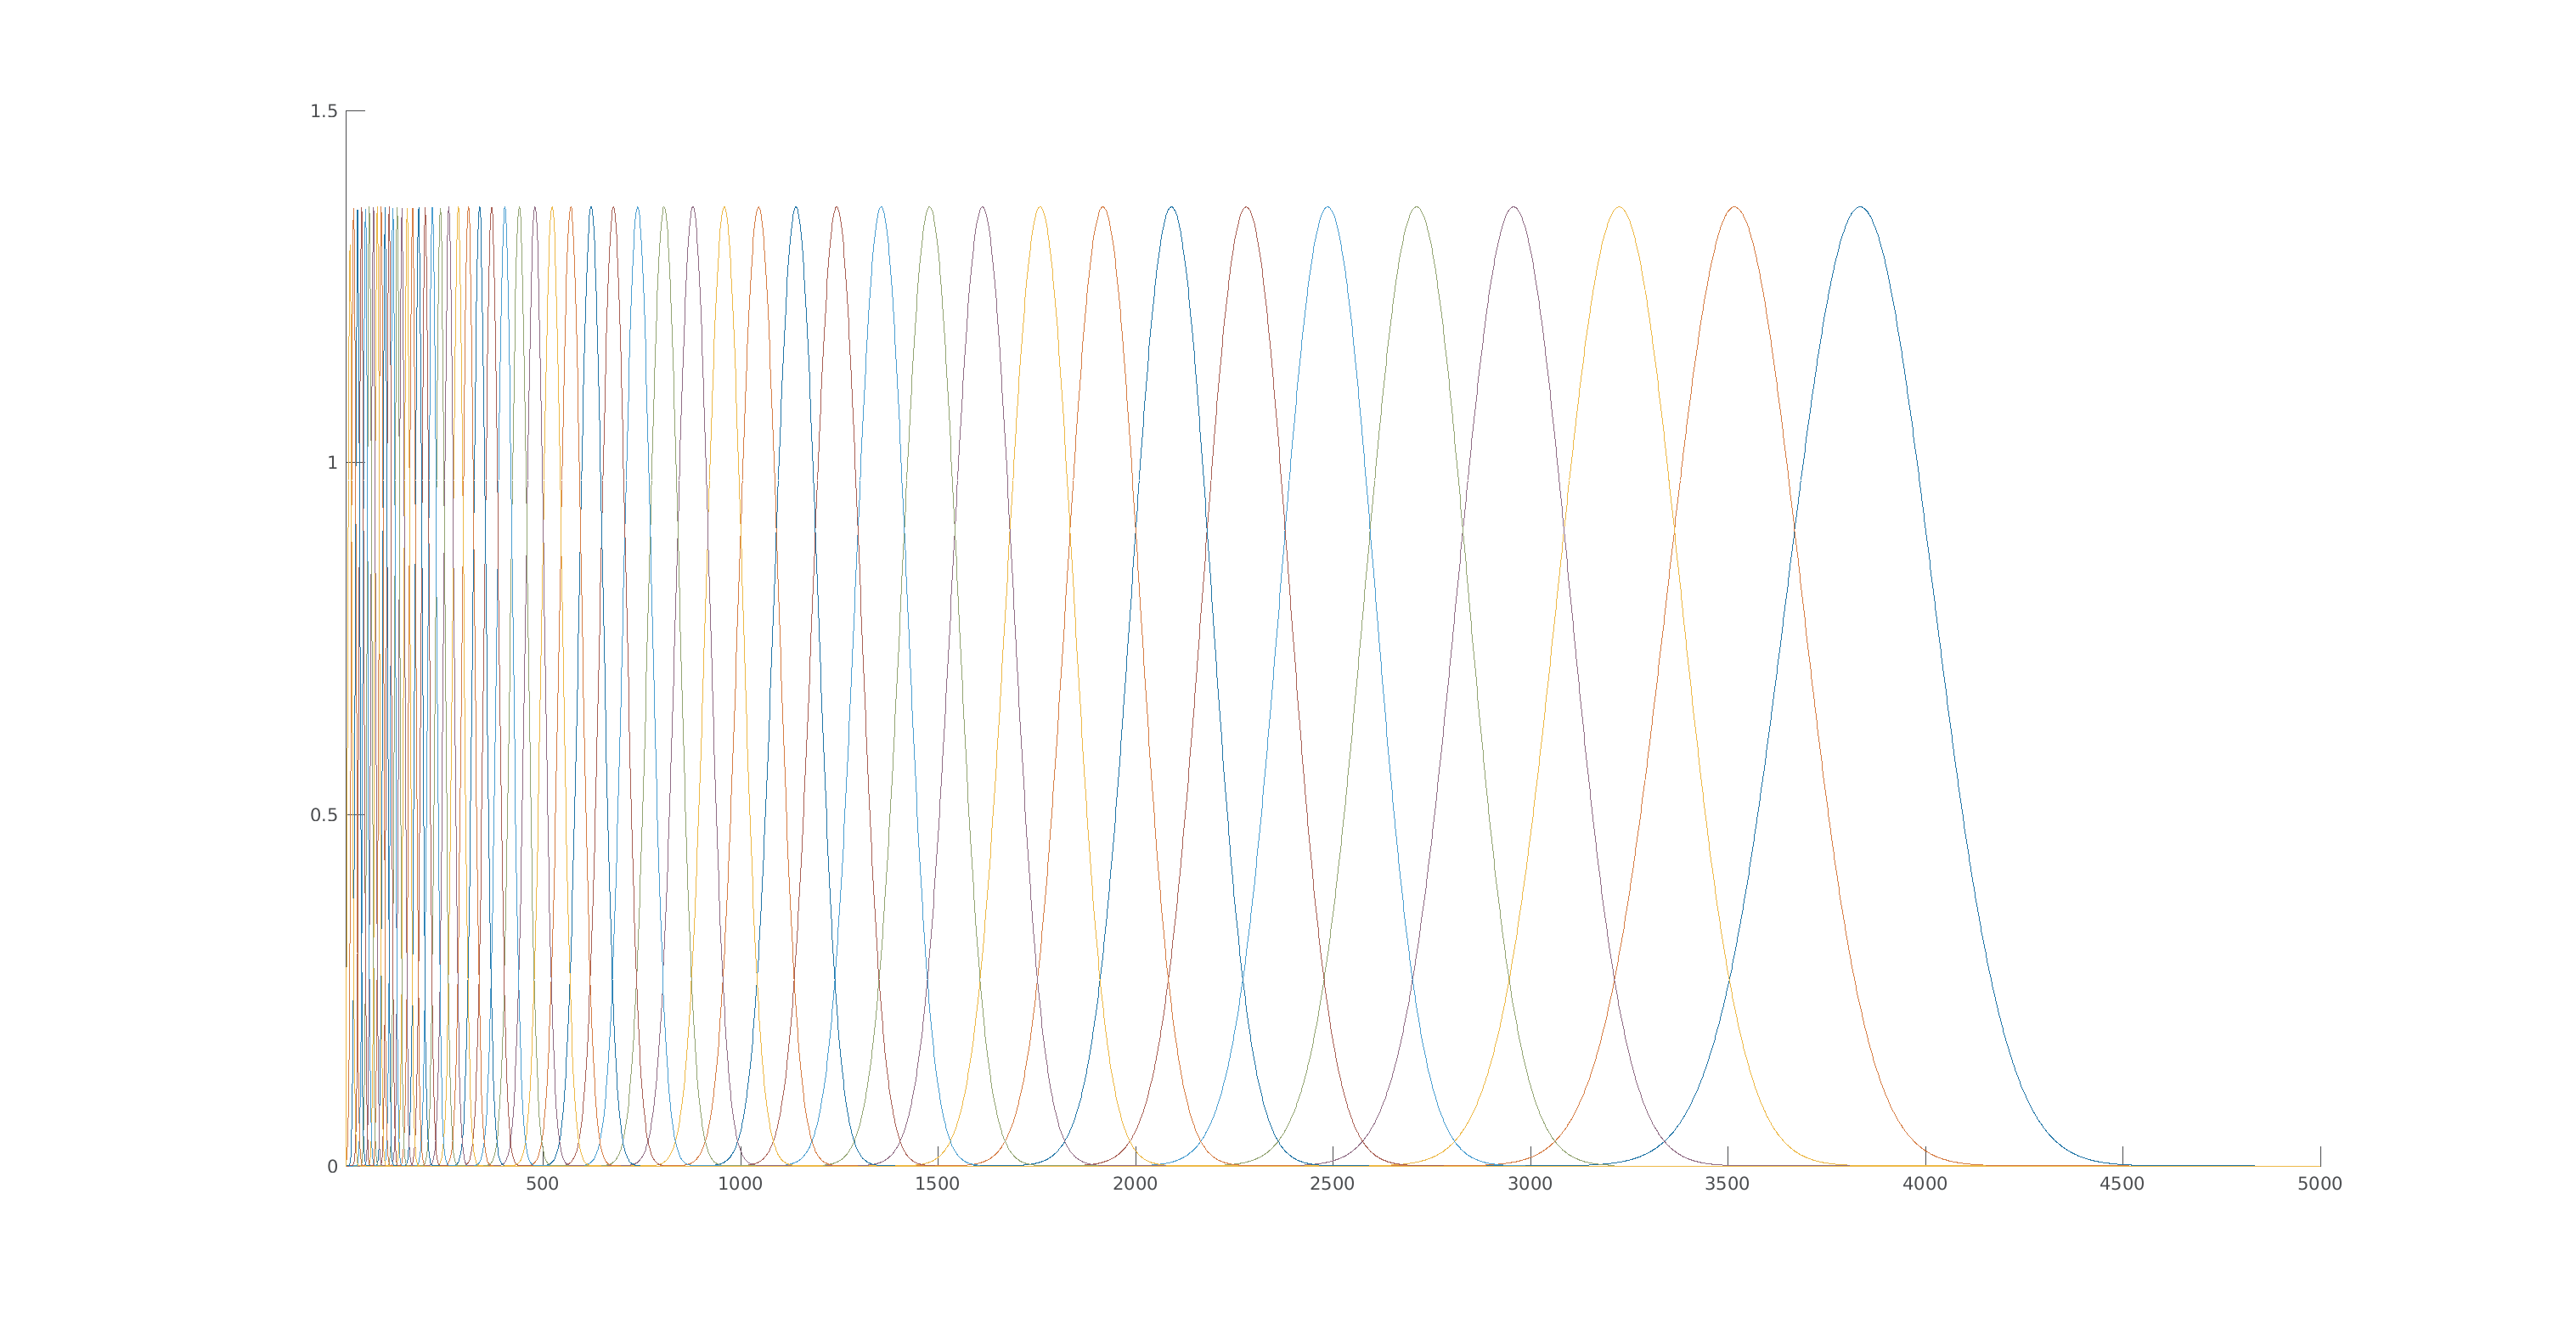
\includegraphics[width=0.9\textwidth]{img/scatter_filters_1.eps}
		\caption{First stage.}
	\end{subfigure}
	\begin{subfigure}[b]{0.45\columnwidth}
		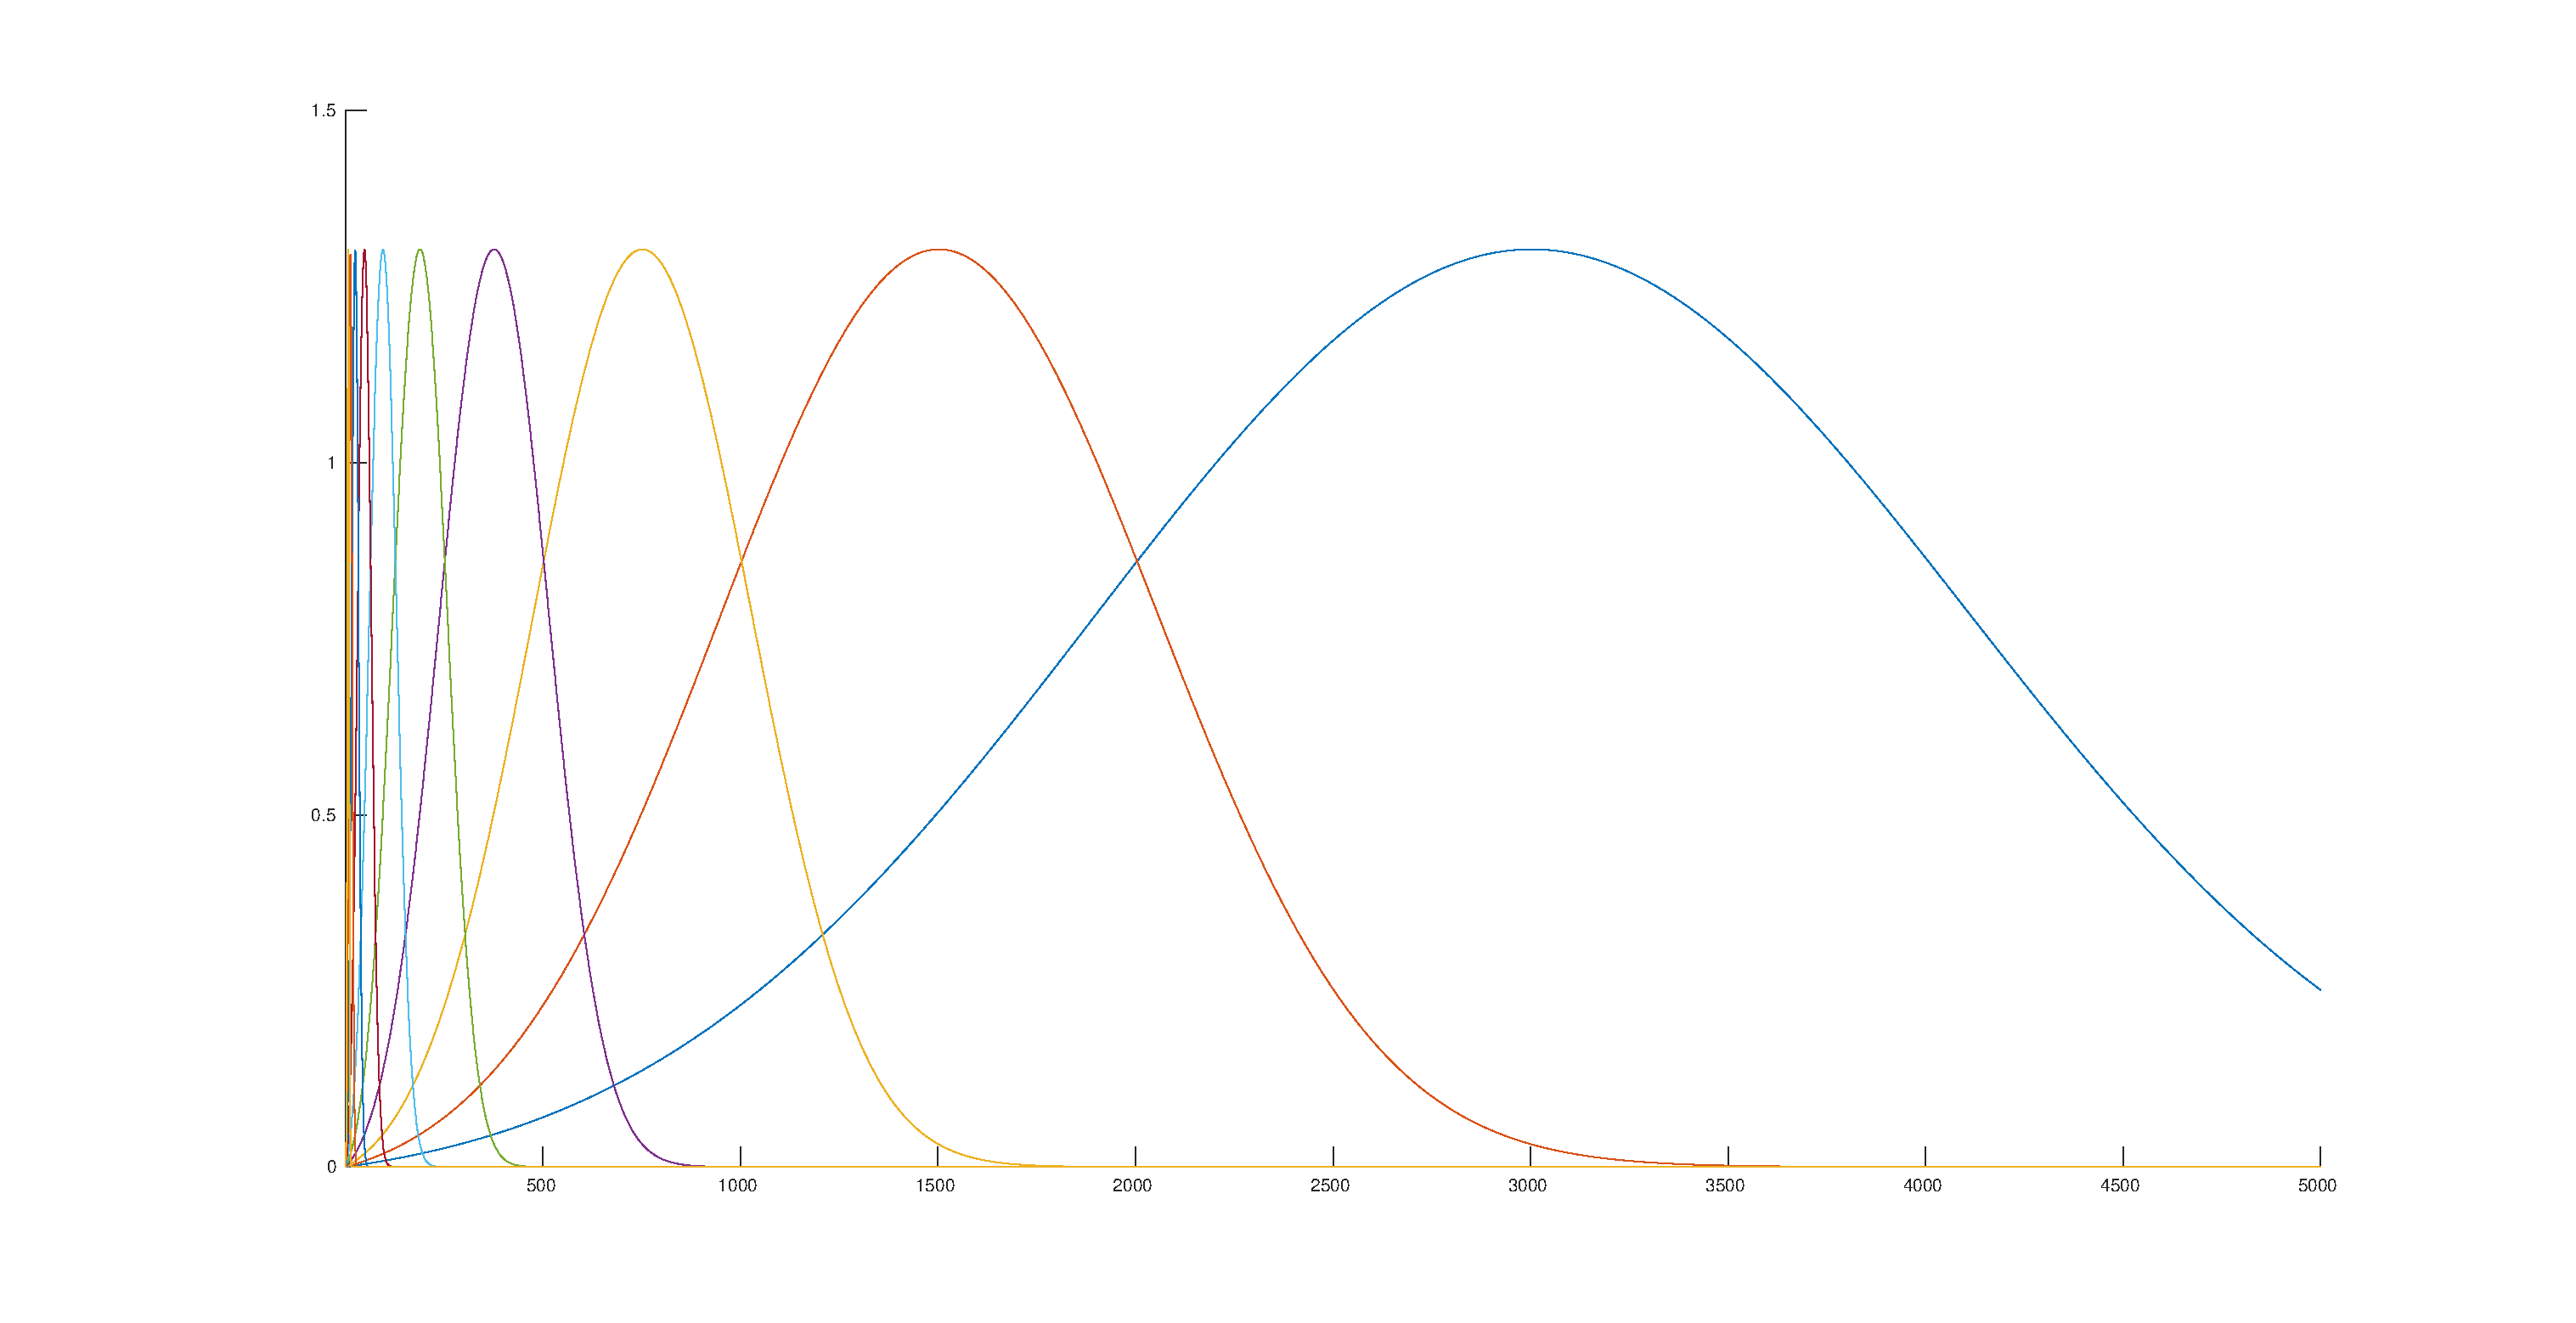
\includegraphics[width=0.9\textwidth]{img/scatter_filters_2.eps}
		\caption{Second stage.}
	\end{subfigure}
	\caption{The Morlet wavelet filterbanks.}\label{fig:filters}
\end{figure}

The mother wavelet $\psi$ may only be dilated up to the maximum scale $M-1$, resulting in 2 wavelets $\psi_{m_0}, \psi_{m_1}$. The parameter $M$ determines the maximum wavelet time support $a^M=T$,
thus the low-pass filter $\phi_M$ covers the interval $[-\pi a^{-M},\pi a^{-M}]$ and represents the length of averaging window over a neighborhood of $t$. 
In this work, we used $T=N/8=1000$ samples, which corresponds to around 60\,ms of audio. 

To improve the classification performance, scattering representation has been processed with the functions of renormalization and logarithmic transformation provided by \textit{ScatNet}. The renormalization consists in dividing second-order scattering coefficients $\mathbf{S}(x_{k,l}, m_2)$ by the first order coefficients $\mathbf{S}(x_{k,l}, m_1)$, in order to decorrelate the amplitudes at the second layer from the first layer. Log-power representation of the frequency distribution is a typical choice in many acoustical classification tasks, thus after the renormalization the logarithm of scattering coefficients is computed. 

For each audio frame, we obtain the SCAT representation $\mathbf{S}(x_{k,l}, M) \in \mathbb{R}^{D \times R}$, where $D=1+52+167=220$ is the total number of scattering coefficients (all orders combined) and $R$ is the number of time points, which is equal to 16. Finally, joining the $\mathbf{S}(x_{k,l}, M)$ for $l=1,\dots,11$ we obtain the deep scattering spectrum of the snore signal $\mathbf{S}(\mathbf{x}_{k}, M) \in \mathbb{R}^{D \times 11\cdot R}$.

\begin{figure}[h]
	\centering
	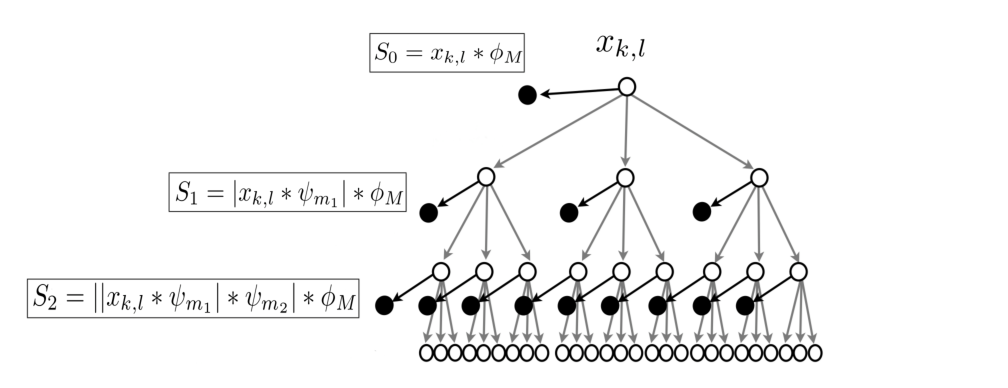
\includegraphics[scale=0.55]{img/scat_spectr_1}
	\caption[SCAT extraction tree]{The SCAT extraction tree. Picture courtesy of And\'{e}n et. al. }
\end{figure}


\subsubsection{Gaussian Mean Supervectors}
A GMS is extracted according to the following procedure. 
Let $\mathbf{s}_r = [\mathbf{S}(\mathbf{x}_{k})]_{*,r}$ the vector of the scattering coefficients of size $D \times 1$ where $r$ is the time point index, the GMM representing an UBM from the training corpus $\mathcal{T}$  is given by:
\begin{equation}\label{eq:ubm}
p(\mathbf{s}_r|\lambda) = \sum_{j=1}^{J}w_j p(\mathbf{s}_r|\boldsymbol{\mu}_j,\boldsymbol{\Sigma}_j),
\end{equation}
where $\lambda=\{w_j,\boldsymbol{\mu}_j,\boldsymbol{\Sigma}_j | j=1,2,\ldots,J\}$, $w_j$ are the mixture weights, and $p(\cdot|\boldsymbol{\mu}_j,\boldsymbol{\Sigma}_j)$ is a multivariate Gaussian distribution with mean vector $\boldsymbol{\mu}_j$ of size $D\times 1$ and diagonal covariance matrix $\boldsymbol{\Sigma}_j$ of size $D \times D$.

The mean values of the UBM model are, then, adapted with the MAP algorithm and concatenated in order to obtain the GMS:

\begin{equation}
\mathbf{\Gamma} = [\boldsymbol{\mu}_1^T,\boldsymbol{\mu}_2^T,\cdots,\boldsymbol{\mu}_J^T]^T,
\end{equation}
where $T$ denotes the transpose operator. Regardless of the length of the input snore sound, $\mathbf{\Gamma}$ is a vector of $DJ\times 1$ length. The threshold values of EM and MAP algorithms during the adaptive phase have been set both equal to 0.001, but with different number of iterations, respectively equal 1000 and 5 for EM and MAP.

\subsubsection{Multi Layer Perceptron}
In this work we exploited the Multi Layer Perceptron (MLP) architecture as DNN Classifier \cite{Rumelhart86-LRB}. The MLP is composed of an input layer with number of units equal to the dimension of the input supervector $\mathbf{\Gamma}$, followed by a stack of fully connected layers of units, namely the \textit{hidden} layers. Number of hidden layers and their dimensions have been investigated during the experimental analysis.
As non-linear activation function in the hidden layers of the MLP we employed both the hyperbolic tangent (\textit{tanh}) and the rectified linear unit (\textit{ReLU}) \cite{Nair2010}.
The output layer of the MLP is formed by four units with the \textit{softmax} non-linear function. 
The outputs of the softmax layer represent the probabilities that a sample belongs to the different classes. 

The  behavior  of  this architecture  is  parametrized  by  the connection weights, which are adapted during the supervised network training, accomplished by using the Adam algorithm \cite{kingma2014adam} for the stochastic gradient-based optimization of the crossentropy loss function. The optimizer parameters were set as follows: learning rate $lr=0.001$, $\beta_1 = 0.9$, $\beta_2 = 0.999$ and $\epsilon = 10^{-8}$. The maximum number of training epochs was set equal to 200 with an early stopping strategy in order to reduce the computational burden. 
Nevertheless, overfitting is well-know a problem affecting DNNs in particular when the number of training samples is limited. In order to prevent overfitting we investigated the use of dropout \cite{srivastava2014dropout}.

The model has been implemented in the Python language using Keras\footnote{https://keras.io/} as deep learning library with Theano\cite{2016arXiv160502688short} as back-end.



\subsection{Comparative Approaches}

Below is given a brief description of state-of-the-art approaches such as SVM classifiers and algorithms which showed the best performance at the Interspeech 2017 ComParE. They were evaluated on the blind \textit{test} set, thus they are reported for comparative aims.

\subsubsection{Support Vector Machines}

Without modifying the general structure of the algorithm for supervectors $\mathbf{\Gamma}$ computation, we compared the performance of the MLP based model with the SVMs \cite{hearst1998support}.

SVMs are binary classifiers that map an input example onto a high-dimensional feature space and iteratively searches for the hyperplane that maximises the distance between the training examples from the origin.  Given the training data $\{\mathbf{\Gamma}_{1},\dots,\mathbf{\Gamma}_{k}\}$, where $k$ is the number of observations, the class separation is performed by solving the following equation:
\begin{align}
\min_{\mathbf{w},\mathbf{\xi},\rho} & \frac{1}{2}\mathbf{w}^T\mathbf{w} + \frac{1}{\nu k}\sum_i \xi_i-\rho \\
\mbox{subject to: } & (\mathbf{w}^T \cdot \Phi(\mathbf{\Gamma}_i)) \ge \rho-\xi_i, \,  \xi_i \ge 0,
\end{align}
where $w$ is the support vector, $\xi_i$ are slack variables, $\rho$ is the offset, and $\Phi$ maps $\mathbf{\Gamma}_i$ into a dot product space $F$ such that the dot product in the image of $\Phi$ can be computed by evaluating a certain kernel function. The kernel function $K(\cdot, \cdot)$ can assume different forms \cite{bishop06}. In this work two kernel functions have been considered, the Radial Basis Function (RBF), defined as:
\begin{equation}
K(\mathbf{\Gamma},\mathbf{\Gamma}_{i}) = \exp(-\gamma \| \mathbf{\Gamma} - \mathbf{\Gamma}_{i}\|^2 )
\end{equation}
and the linear kernel, defined as:
\begin{equation}
K(\mathbf{\Gamma},\mathbf{\Gamma}_{i}) = \mathbf{\Gamma}^T\mathbf{\Gamma}_{i}.
\end{equation}
The decision values are obtained with the following function:
\begin{equation}
\label{eq:hyper}
f(\mathbf{\Gamma}) = \mathbf{w}^T \cdot \Phi(\mathbf{\Gamma})-\rho.
\end{equation}
The input vector $\mathbf{\Gamma}$ is classified as $+1$ if $f(\mathbf{\Gamma}) \geq 0$ and $-1$ if  $f(\mathbf{\Gamma}) < 0$.
In this work, the multiclass problem has been addressed using the ``one versus all'' strategy. Implementation of LIBSVM \cite{chang11} from Python library \textit{scikit-learn} has been employed both in the training and testing phases of the SVM.

\subsubsection{Weighted Kernel Classifiers}
The approach  proposed by Kaya and Karpov \cite{kaya2017introducing} exploits a decision fusion between different kernel based classifiers such as regular and weighted Kernel Extreme Learning Machine (KELM) and Kernel Partial Least Squares (KPLS) learners.
As acoustic feature representation they used Fisher Vectors (FV), which provides an encoding of local descriptors (e.g., MFCC, RASTA-PLP and their derivatives), quantifying the gradient of the parameters of the background model with respect to the data. In addition, in the final submission system they used both (FV) and the ComParE baseline feature set, which contains 6373 static features resulting from the computation of various functionals over low-level descriptor (LLD) contours.  

\subsubsection{Image-based Deep Spectrum Features}
A different approach is presented in \cite{amiriparian2017snore}, based on image classification convolutional neural network (CNN) descriptors extracted from snore spectrograms. They evaluated different well known DNN architectures typically used for image classification, such as AlexNet and VGG neural network. Both deep CNNs were previously trained on approximately 1.2 million images from the ImageNet corpus, then they compute the power spectral density on the dB power scale of the audio excerpt using Hanning windows of 16 ms width, and 8 ms overlap and they plotted the result in three different colour maps: gray, jet and viridis. The deep CNNs are fed with the spectrograms, then the neurons on the first and second fully connected layers (fc6 and fc7) are extracted as feature vectors. These feature vectors are then classified by means of an SVM model. 

\subsection{Experiments}

\subsubsection{The MPSSC dataset}
\label{ssection:MPSSCdataset}
The MPSSC dataset is composed of more than 30 hours of audio recordings captured during DISE examinations of 224 subjects from three medical centers recorded between 2006 and 2015. Recording equipment, microphone type, and location differ among the medical centers, so do the background noise characteristics. From the original signals (raw PCM, sample rate 16\,000\,Hz, quantization 16 bit) 843 early identifiable, single site of vibration snore events have been extracted and manually screened from medical experts.
Following the 4-class VOTE scheme, each sound file in the dataset is labelled as V, O, T, E, depending on the tissue from which snore sound originates, as shown in \figref{fig:vote}. They are respectively:
\begin{itemize}
	\itemsep1mm
	\item (V) - Velum (palate), including soft palate, uvula, lateral velopharyngeal walls;
	\item (O) - Oropharyngeal lateral walls, including palatine tonsils;
	\item (T) - Tongue, including tongue base and airway posterior to the tongue base;
	\item (E) - Epiglottis.
\end{itemize}


The dataset is divided into three subsets: \textit{train}, \textit{devel} and \textit{test}.
The number of events per class in the database is strongly unbalanced with a high preeminence of the ``Velum'' (V)-class  and ``Oropharyngeal'' (O)-class (85\% of samples) but in line with the likelihood of occurrence during normal sleep, while 10\% and 5\% of samples respectively belongs to E-events and T-snores. Details of class occurrences are shown in Table I.

\begin{table}[h]
	\centering
	\begin{tabular}{cccc}
		\toprule
		\multicolumn{4}{c}{\textbf{The Munich-Passau Snore Sound Corpus}} \\
		\midrule
		\#  \rule{10pt}{0pt}	& train  \rule{10pt}{0pt} & devel & test\\
		\midrule
		V \rule{10pt}{0pt}	& 168  \rule{15pt}{0pt} & 161 & 155\\
		O \rule{10pt}{0pt}	& 76  \rule{15pt}{0pt} & 75 & 65\\
		T \rule{10pt}{0pt}	& 8  \rule{15pt}{0pt} & 15 & 16\\
		E \rule{10pt}{0pt}	& 30  \rule{15pt}{0pt}& 32 & 27\\
		\bottomrule
		$\Sigma$  \rule{10pt}{0pt} & 282  \rule{13pt}{0pt} & 283 & 263\\
	\end{tabular}
	\caption[The Munich-Passau Snore Sound Corpus]{The Munich-Passau Snore Sound Corpus - The table shows the number of events per class in train, devel and test.}
	\label{tab:mpssc} 
\end{table}

As shown in the waveforms and the related spectrograms in \figref{fig:vote_spectrograms}, the main energy components in three of the classes are concentrated in the frequency area below around 2000 Hz. Energy and spectral distribution characteristics are similar, except for the Type T, which shows higher energy content above 2500 Hz compared to the other three.

\begin{figure*}[h]
	\centering
	\begin{subfigure}{.4\textwidth}
		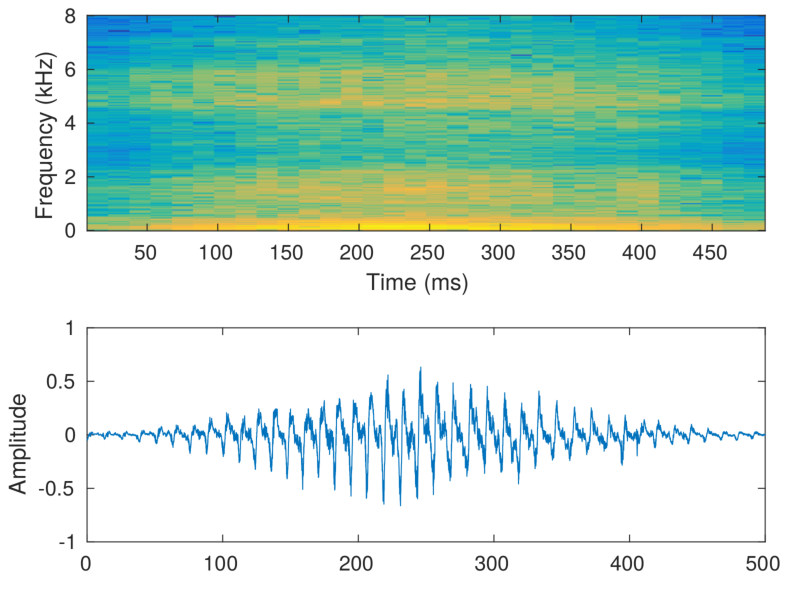
\includegraphics[width=\linewidth]{img/V_spec_crop.pdf}
		\caption{}
		\label{fig:V}
	\end{subfigure}
	\begin{subfigure}{.4\textwidth}
		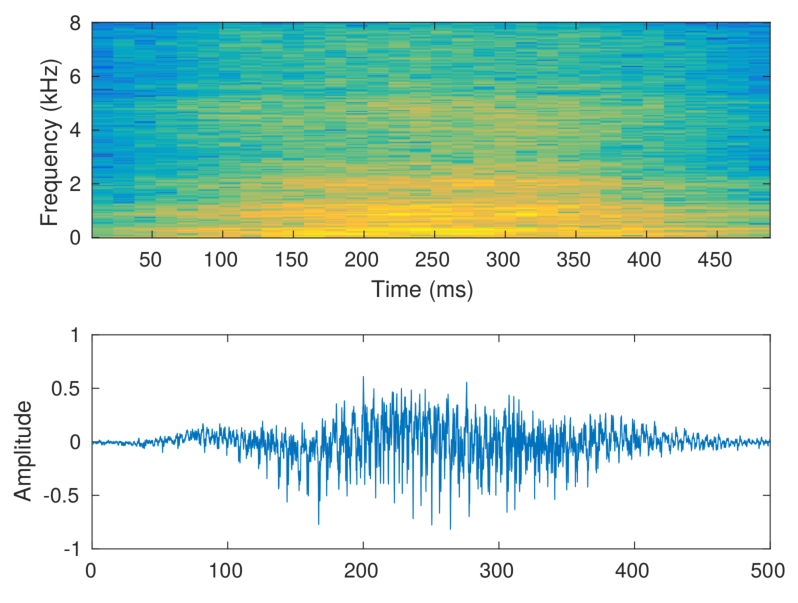
\includegraphics[width=\linewidth]{img/O_spec_crop.pdf}
		\caption{}
		\label{fig:O}
	\end{subfigure}
	\begin{subfigure}{.4\textwidth}
		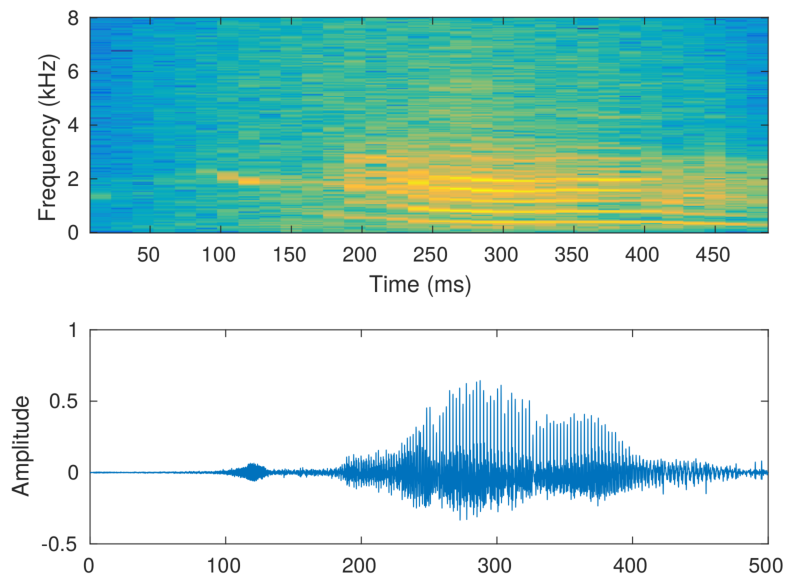
\includegraphics[width=\linewidth]{img/T_spec_crop.pdf}
		\caption{}
		\label{fig:T}
	\end{subfigure}
	\begin{subfigure}{.4\textwidth}
		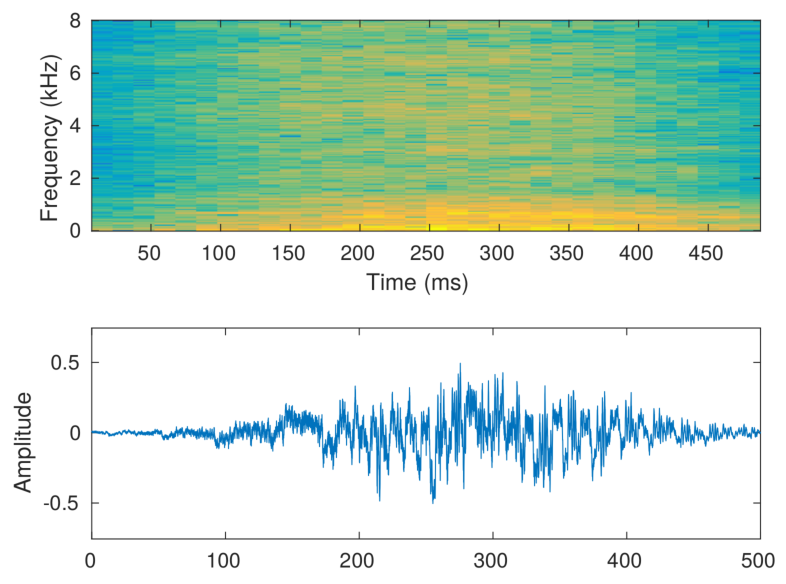
\includegraphics[width=\linewidth]{img/E_spec_crop.pdf}
		\caption{}
		\label{fig:E}
	\end{subfigure}
	\caption[Spectrograms of VOTE sounds]{Waveforms and spectrograms of VOTE events}{(a) V (velum); (b) O (oropharyngeal); (c) T (tongue base); (d) E (epiglottis).}
	\label{fig:vote_spectrograms}
\end{figure*}


\subsubsection{Experimental Setup}
According to the ComParE 2017 guidelines \cite{ComParE2017}, the performance metric for this task is the Unweighted Average Recall (UAR) which is defined as:
\begin{equation}
UAR= \frac{1}{NClass} \cdot \sum_{c=1}^{NClass}\frac{TP_c}{TP_c+FN_c}
\end{equation}

The MLP hyperparameters optimization was obtained by means of a \textit{random search} strategy  \cite{bergstra2012}.  The number of layers, the number of units per layers, the non-linear activation function and the dropout rate have been varied for a total of 400 configurations. Details of searched hyperparameters and their ranges are reported in Table II. For all of the configurations, the performance of the MLP classifier has been evaluated by varying the input supervector dimension, which depends on the number of Gaussian components used to represent the UBM $J={1,2,4,8}$. The supervector given as input to the MLP is standardized by removing the mean value of each $\boldsymbol{\mu}_j$ component and scaled by dividing for their standard deviation. 
\begin{table}[h]
	
	\centering
	\begin{tabular} {|c | c | c|}
		\hline
		Parameter & Range & Distribution\\  
		\hline
		\hline                                     
		MLP layers Nr.  & [2 - 5]& uniform \\
		\hline                                     
		MLP layers dim. & [20 - 256]& log-unifom \\
		\hline                                     
		Activation & [$tanh$ - ReLU] & uniform\\
		\hline
		Dropout Rate & [0.5 - 0] & uniform \\
		\hline
	\end{tabular}		
	\caption[VOTE Classification - Experiments]{Hyper-parameters optimized in the random-search phase for the MLP classifier, and their range.}
	\label{tab:randomsearch}
\end{table}

Regarding the SVM classifier optimization, we conducted a preliminary analysis which showed that in this task the linear kernel function provides better performance with respect to the RBF kernel.
Then, with a grid search strategy  we explored the SVM penalty parameter $C$ which yielded the best results. In particular, $C$ assumed the values $2^{-15}, 2^{-14},\ldots,2^{15}$ for a total of 30 different values. The supervectors at the input of the SVM were scaled to the range $[-1,1]$.

During the training procedure of both classifiers, different weights were given to samples belonging to different classes in order to counteract the dataset unbalancing. The weight for each class was computed on training set with the following equation:
\begin{equation}
W_c = \frac{N_{TOT}}{N_c},
\end{equation}
where $N_{TOT}$ is the total number of samples in the training set and $N_c$ the number of samples of the respective class. In this way the classes having a lower number of samples in the training set have a larger effect in the loss computing \cite{king2001logistic}. 

\subsection{Results}

The performance of the proposed algorithm has been assessed firstly by using the \textit{train} subset as training corpus and the \textit{devel} subset for evaluation. Then, the same model was trained with both \textit{train} and \textit{devel} subsets and it was evaluated on the \textit{test} subset. The results of the experiments are shown in Table III. For the sake of conciseness  only the best performances of the proposed approach are reported, comparing the results achieved with SVM and MLP classifiers on the two folds. For both \textit{devel} and \textit{test} subsets the best results are obtained with DNN based classifier.

\begin{table*}[h]
	\centering
	\resizebox{\textwidth}{!}{  
	\begin{tabular}{ c|c|c | c }
		\hline
		\textbf{Input} \rule{0pt}{10pt} & \textbf{Classifier}  & \textbf{UAR devel (\%)} & \textbf{UAR test (\%)} \\ 
		\hline
		SCAT \rule{0pt}{8pt}&  MLP [204,112,99]   & \multirow{2}{*}{53.16} & \multirow{2}{*}{72.63}\\
		+ 1 Gaussian UBM 							& with $tanh$ and dropout &							&									\\	
		\hline
		SCAT \rule{0pt}{8pt}&  MLP [249,40,21,21]   & \multirow{2}{*}{58.20} & \multirow{2}{*}{\textbf{74.19}} \\
		+ 2 Gaussians UBM 							& with $tanh$ and dropout &							&									\\	
		
		\hline
		SCAT \rule{0pt}{8pt}& MLP [235,227]   & \multirow{2}{*}{\textbf{67.14}} & \multirow{2}{*}{67.71} \\
		+ 2 Gaussians UBM 							& with $tanh$ and dropout &							&									\\	
		\hline
		SCAT \rule{0pt}{8pt}&  MLP [156,34,21]   & \multirow{2}{*}{50.30} & \multirow{2}{*}{71.32} \\
		+ 4 Gaussians UBM 							& with $relu$ and dropout &							&									\\	
		\hline
		SCAT \rule{0pt}{8pt}&  MLP [66,28]   & \multirow{2}{*}{55.89} & \multirow{2}{*}{70.18} \\
		+ 8 Gaussians UBM 							& with $tanh$ and dropout &							&									\\	
		\hline
		SCAT \rule{0pt}{8pt} & \multirow{2}{*}{SVM, $C=2^{-8}$} & \multirow{2}{*}{46.73} & \multirow{2}{*}{65.45} \\
		+ 1 Gaussian UBM & 						&							&									\\
		\hline
		SCAT \rule{0pt}{8pt} & \multirow{2}{*}{SVM, $C=2^{-10}$} & \multirow{2}{*}{46.54} & \multirow{2}{*}{65.50} \\
		+ 2 Gaussian UBM & 						&							&									\\
		\hline
		SCAT \rule{0pt}{8pt} & \multirow{2}{*}{SVM, $C=2^{-9}$} & \multirow{2}{*}{44.67} & \multirow{2}{*}{67.22} \\
		+ 4 Gaussian UBM & 						&							&									\\	
		\hline
		SCAT \rule{0pt}{8pt} & \multirow{2}{*}{SVM, $C=2^{-10}$} & \multirow{2}{*}{43.20} & \multirow{2}{*}{65.48} \\
		+ 8 Gaussian UBM & 						&							&									\\	
		\hline
		%		\hline
		%		Spectrograms + AlexNet fc7 					\rule{0pt}{8pt} & SVM	&		44.80 & 67.00 \\
		%		\hline
		%		FV and ComParE functionals	& Fusion KPLS, WKPLS, KELM and WKELM & 50.12 & 64.23  \\
	\end{tabular}
	}
	\caption[VOTE Classification - Results]{Comparative results in terms of UAR (\%) score of proposed method for MLP and SVM based classifiers for both \textit{devel} and \textit{test} subsets. Best results on each subset are shown in \textbf{bold}.}
	\label{tab:results1}
	
\end{table*}


\subsubsection{Results on \textit{devel} subset}
On this subset the best MLP topology resulting from the random search is composed of 2 hidden layers with respectively ${235,227}$ units, $tanh$ as non linear activation function and a dropout rate equal to 0.5. The network input consists of supervectors originated from UBM with 2 gaussian components, thus the input size is equal to $440 \times 1$. This architecture provides an UAR up to 67.14\%. Regarding the SVM based classifier, the best performing model on \textit{devel} subset is fed with a supervector mapped on a UBM of 1 gaussian component and with the parameter $C=2^{-8}$ obtain an UAR equal to 46.73\%.
The corresponding confusion matrices are illustrated in \figref{fig:cm_devel}, which exhibits for the MLP (\figref{fig:cm_devel_mlp}) the higher recall (80.00\%) for the minority class (T), but a moderate recall (53.12\%) for the second smallest class (E). The SVM based classifier obtains the highest recall on the (E) class, while the other classes obtain worse performance. The superiority of the DNN based classifier is motivated by its well known ability to encode in the inner structure the features of the different snore sounds highlighted by the SCAT and better distinguish the samples, notwithstanding the large unbalancing of the dataset. 

\begin{figure}[h]
	\centering	
	\begin{subfigure}{.4\textwidth}
		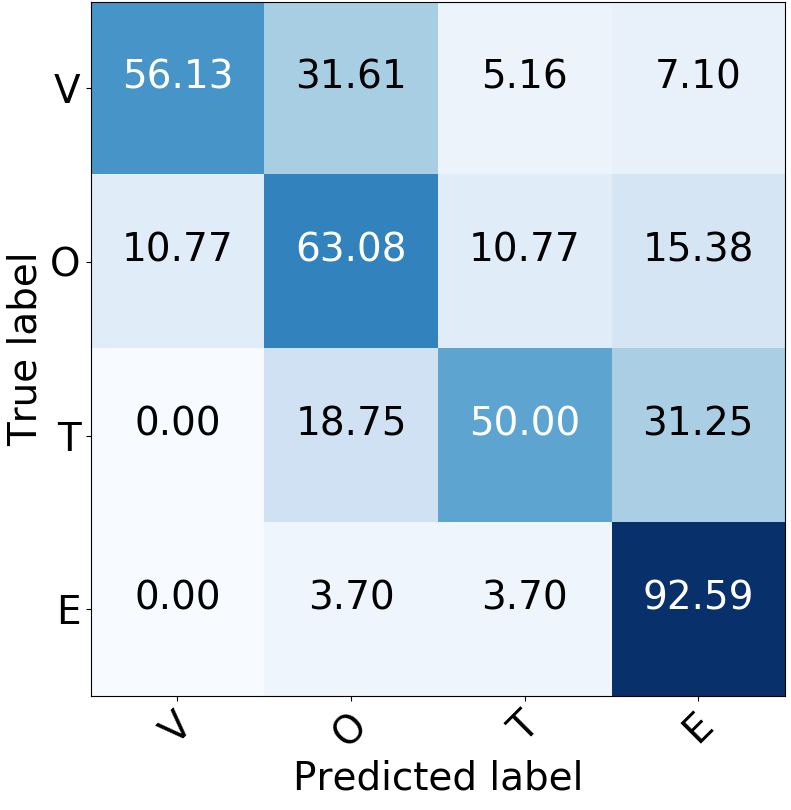
\includegraphics[width=\linewidth]{img/cm_devel_svm.png}
		\caption{}
		\label{fig:cm_devel_svm}
	\end{subfigure}
	\begin{subfigure}{.4\textwidth}
		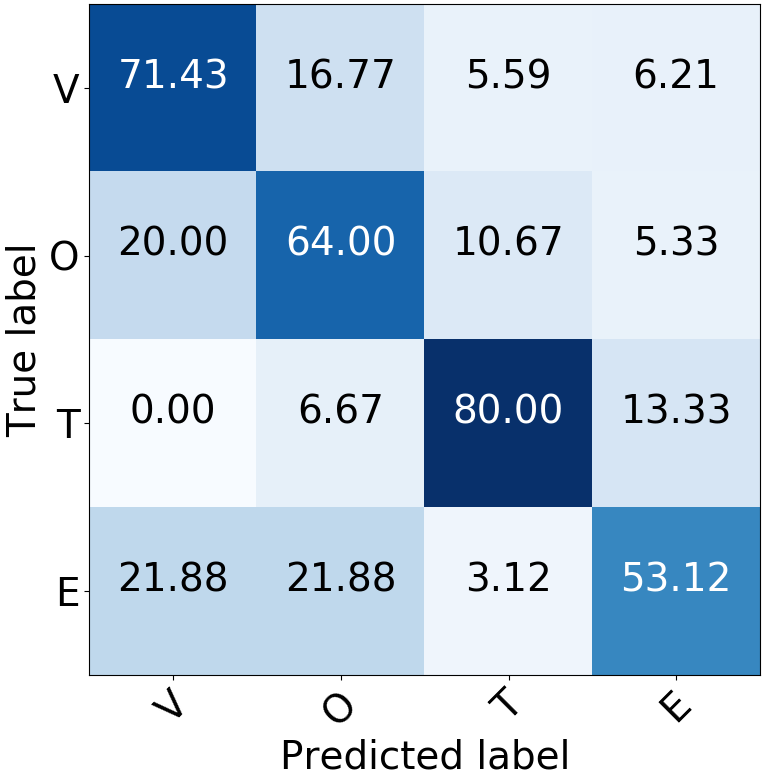
\includegraphics[width=\linewidth]{img/cm_devel_mlp.png}
		\caption{}
		\label{fig:cm_devel_mlp}
	\end{subfigure}
	\caption[VOTE Classification - Devel set results]{Normalized confusion matrix of best performing models on \textit{devel} subset. (a) SVM Classifier, (b) MLP Classifier.} 
	\label{fig:cm_devel}
\end{figure}


\subsubsection{Results on \textit{test} subset}
The network topology achieving the absolute best results optimized on \textit{test} subset is composed of 4 hidden layers with respectively ${249, 40, 21, 21}$ units, $tanh$ as non linear activation function and a dropout rate equal to 0.5. As in the case of \textit{devel} subset the input size is equal to $440 \times 1$, consisting of supervectors originated from UBM with 2 gaussian components. This architecture shows an UAR up to 74.19\%. The SVM model which obtains the best performance is fed with supervectors mapped on 4 gaussians UBM and a parameter $C=2^{-10}$. The respective UAR is equal to 67.22\%.
The obtained confusion matrices are illustrated in \figref{fig:cm_test}. In this case the augmented number of samples has a beneficial effect on the recall score of almost all the four classes for the MLP classifier, while the performance of SVM classifier are similar to the \textit{devel} subset.

\begin{figure}[h]		
	\centering
	\begin{subfigure}{.4\textwidth}
		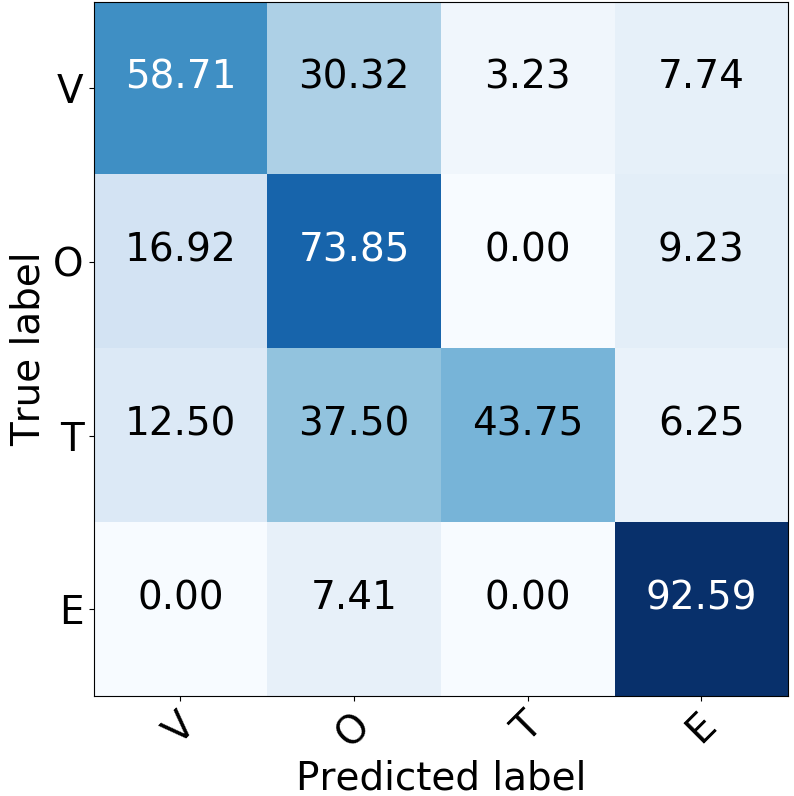
\includegraphics[width=\linewidth]{img/cm_test_svm.png}
		\caption{}
		\label{fig:cm_test_svm}
	\end{subfigure}
	\begin{subfigure}{.4\textwidth}
		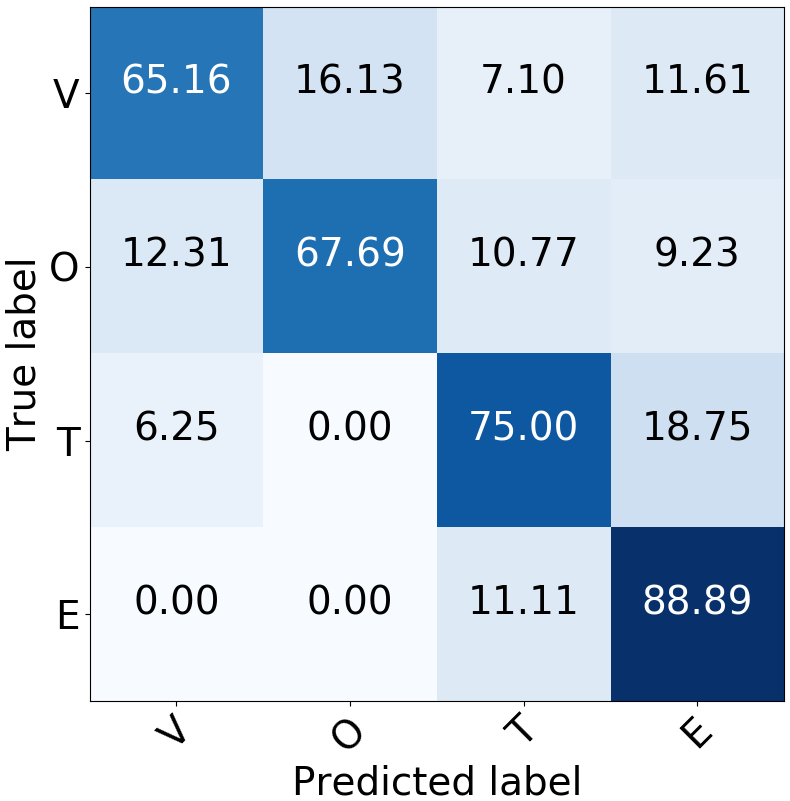
\includegraphics[width=\linewidth]{img/cm_test_mlp.png}
		\caption{}
		\label{fig:cm_test_mlp}
	\end{subfigure}
	\caption[VOTE Classification - Test set results]{Normalized confusion matrix of the best performing models on \textit{test} subset. (a) SVM Classifier, (b) MLP Classifier.} 
	\label{fig:cm_test}
\end{figure}

\subsubsection{Comparative Results}
In Table IV the best performance obtained with presented methods in \cite{kaya2017introducing}, which resulted the winner of the ComParE challenge, and in \cite{amiriparian2017snore} are reported. The best UAR score on both the subsets is provided by our proposed algorithm relying on DNN classifiers. The absolute improvement on the state-of-the-art methods on the \textit{devel} subset is remarkable, in fact we obtain in terms of UAR +17.02\%. For a fair comparison on the \textit{test} partition we have to consider the score obtained with the best model on the \textit{devel} set. In this case our proposed algorithm overcome the UAR scores of +3.48\% and +0.71\% with respect to \cite{kaya2017introducing} and \cite{amiriparian2017snore}. This results highlight that the best performance obtained on \textit{devel} set do not provide at the same time the best performance on the \textit{test} set, as it also emerged from the challenge results of reported methods. The motivation of these low generalization proprieties probably relies on the dataset splits composition and their class unbalancing. 
Anyway, the obtained performances encourage the use of SCAT as snore sound features which results to be effective. In addition, the combination of SCAT and GMS allows reduce dimension of the input vector of the classifier and to obtain an higher classification accuracy with respect to state-of-the-art methods.

\begin{table}[ht]
	\centering
	\begin{tabular}{|c|c|c|c|}
		\hline
		\multirow{2}{*}{\textbf{Input}} \rule{0pt}{10pt} & \multirow{2}{*}{\textbf{Classifier}} & \multicolumn{2}{c|}{\textbf{UAR (\%)  }}\\
		\cline{3-4}
		&  & \textbf{\textit{devel}} & \textbf{\textit{test}} \\ 
		\hline
		SCAT \rule{0pt}{8pt} &  MLP   & \textbf{67.14} & 67.71 \\
		\hline
		SCAT \rule{0pt}{8pt} &  MLP   & 58.28 & \textbf{74.19} \\
		\hline
		Spectrograms + \rule{0pt}{8pt} & \multirow{2}{*}{SVM}	& \multirow{2}{*}{44.80} & \multirow{2}{*}{67.00} \\
		AlexNet fc7						&						&						&						   \\
		\hline
		FV + 	& (W)KPLS + & \multirow{2}{*}{50.12} & \multirow{2}{*}{64.23}  \\
		ComParE functionals &  (W)KELM  & 				&						\\
		\hline
	\end{tabular}
	\caption[VOTE Classification - Comparative Results]{Comparative results in terms of UAR (\%) score of proposed algorithm with state-of-the-art methods for both \textit{devel} and \textit{test} subsets. Best results on each subset are shown in \textbf{bold}.}
	\label{tab:results2}
\end{table}


\subsection{Conclusion and Outlook}
\label{section:concl}

In this work, an approach for snore sound classification based on Deep Scattering Spectrum, Gaussian Mean Supervectors and MLP classifier has been presented. We extracted the SCAT from the audio signals and GMM-based background model was trained to map the sequence of scattering coefficients in a supervector. Classification of input snore sounds has been performed using a MLP neural network and a support vector machine with comparative aims. To assess the performance of the algorithm we conducted experiments on both the \textit{devel} and the \textit{test} subsets of MPSSC dataset.
Following the 4-class VOTE scheme, we obtained a UAR of 67.14\% on the \textit{devel} set and a respective UAR equal to 67.71\% on the \textit{test} set independently of the subject characteristics. 
The performance upper limit obtained optimizing the models on the \textit{test} set is an UAR up to 74.19\%.
The obtained results showed that the employment of the DNN based classifier in combination with SCAT is effective and a significant performance improvement with respect to other state-of-the-art approaches was registered. 
Future work will evaluate strategies of data augmentation to counteract the unbalance of the dataset. In addition, the SCAT representation of the audio signals prompts the exploitation of the 2-D Convolutional neural network (CNN) to obtain a further latent representation by means of the processing taking place in its deep architecture.
A deeper focus will be given also to the temporal evolution of the signal by means of recurrent structure, such as Long Short Term Memory (LSTM) Neural Networks \cite{graves2005framewise}. 
\newpage






%%%%%%%%%%%%%%%%%%%%%%%%%%%%%%%%%%%%%%%%%%%%%%%%%%%%%%%%%%%%%%%%%%%%%%%%%%%%%%%%%%%%%%%%%%%%%%%%%
\section{Road Surface Roughness Classification}
	
	\begin{figure}[h]
		\centering
		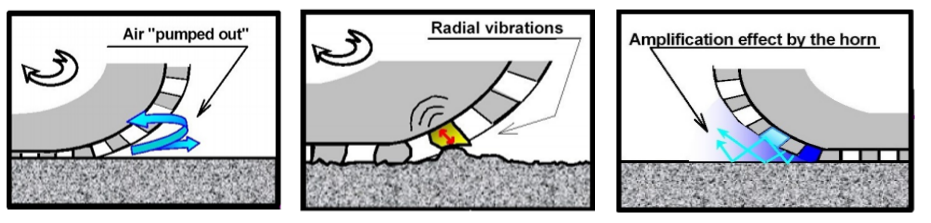
\includegraphics[width=\textwidth]{img/pompaevibrazionihorn.png}
		\caption[Tyre-Road Noises]{The tyre-road noise generation. Left:  Air pumping at the entrance of the contact patch; Center: Vibration caused by tread/block pavement impact; Right: The horn effect created by the tyre and road.}
		\label{fig:tyre-road-noise}
	\end{figure}
	
The aim of this work is to develop an automatic system for the road roughness classification. As first step was conducted an accurate state of the art analysis.	
Vehicle noise emissions depend on multiple factors, including the power unit noise, aerodynamic noise and tyre-road noise \cite{hanson2004tire}. They are all dependent on speed but have different behaviors. The power unit noise, for instance, depends on the gear engaged and the number of revolutions per minute whereas the tyre-road noise is proportional to the logarithm of the vehicle speed. The balance between these two noise contributions depends, thus, on speed. 
At low speeds the power unit noise dominates the roadside noise levels, while at high speeds the tyre/road is the predominant source of noise. In \cite{sandberg2001tyre} it is shown that  the tyre-road noise component becomes predominant with modern cars even at speeds above 30 km/h, regardless of the engaged gear. 

The tyre-road noise, results from the sum of several acoustic phenomena that concur to the noise emission. The source generation mechanism includes the following elements: 
\begin{itemize}
	\item  \textit{Tread Impact}: at the entrance of the interface between tyre and pavement (referred to as contact patch) an impact occurs as the tread hits the pavement. This impact causes vibration of the tyre carcass. 
	\item \textit{Air Pumping}: within the contact patch, the passages and grooves in the tyre are compressed and distorted. The air entrained in this passages will be compressed and pumped in and out of the passages. This  rapid exit of air can lead to sound generation.
	\item \textit{Horn Effect}: sound emitted from the tyre/road contact is reflected multiple times between the road surface and the tyre tread before it propagates further to the receiver. The tyre/road geometry has the shape of a horn. This horn shape causes a much larger radiation efficiency of the emitted tyre/road noise than in free field. This increased radiation efficiency is referred to as the horn effect. 
\end{itemize}	

\begin{figure}[h]
	\centering
	\centerline{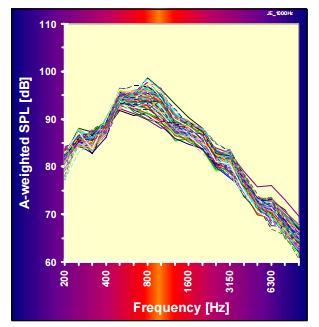
\includegraphics[width=0.45\textwidth]{img/tire.png}}
	\caption[Third-octave band noise spectra]{Third-octave band spectra obtained in TUG/VTI project for 50 different car aftermarket tyres running on the TUG drum at 90 km/h.}
	\label{fig:noise-spec}
\end{figure} 


Noise spectra have been measured on a large number of tyres (about 50) \cite{sandberg2003multi} in a cooperation project between the Technical University of Gdansk (TUG) in Poland and the Swedish National Road and Transport Research Institute (VTI). Despite a wide range of tyre types, the spectral shapes are very similar and the sound concentrates around a peak at 800-1000 Hz. 
Several studies \cite{freitas2009traffic} carried out in roads with different types of surface and age have usually shown that dense asphalt concrete and stone mastic asphalt are the ones that generate more noise contrasting with double and single porous asphalt. Porous pavements are constructed by reducing the amount of small aggregate used in the pavement
such that the pavement cannot be tightly compacted. In general, porous pavement reduces tyre/pavement interaction noise above 1000 Hz. Porosity reduces the strength of the air pumping source mechanism by preventing air compression and reduces the enhancement potential of the horn effect as shown in \figref{fig:noise-spec}. 
Some tests \cite{hanson2004tire} done in Colorado provide a preliminary understanding of the effect of pavement age on noise level. The results shows that, as expected, the older the pavement, the higher the noise level.

In this work we are interested in inferring the surface roughness by analyzing the near-field acoustic emissions of the vehicle. The surface roughness is characterized by the average size of the gravel base and the presence of filling (asphalt concrete or concrete). These elements have a large impact on the noise emission level and character. 


\subsubsection{Related Works}

A recent paper \cite{DoganRoad2017}, reports on the use of Support Vector Machines for the goal of classifying several types of road (asphalt, gravel, snow, stony road) using acoustic features. The work employs an electric car for minimal impact of the engine noise on the recording and collects 30 audio fragments from different roads at a fixed speed of 20km/h. The work employs MFCC as they were shown to maximize the Kullback-Leibler distance between all the audio fragments. Classification with the MFCC and an SVM are rather high (between 92.5\% and 97.5\%), however they decrease to 67\%-89\% when noise is artificially added to the recordings (such as rain noise or the noise of another car passing by).
SVM are employed also in \cite{alonso2014board}, where the main goal, however, is the classification of the road surface wetness and the feature extraction is done with selected 1/3 octave band filters. In that work the recordings are taken in a closed circuit with an internal combustion engine vehicle.
A different approach for road dry/wet classification is undertaken in \cite{abdic2016detecting} where a dataset is built from recordings of road trips in the US lasting tens of minutes on different types of asphalt in both dry and wet conditions. The work performs classification using a Bi-Directional Long-Short Term Memory (BLSTM) neural network \cite{hochreiter1997long} and Auditory Spectral Features (ASF). The paper reports a unweighted average recall of 93.2\% as best result, with a large improvement over \cite{alonso2014board}.

These works motivate us to investigate deep learning approaches for the road surface detection problem. In-car equalization profiles may be determined on the basis of the estimated surface roughness in order to improve the listening quality in the cockpit or to obtain suggestions on the driving experience. We propose to extract audio features for the classification of road roughness in two classes corresponding to two extremes. Owing from previous works we build a corpus of data to train an efficient neural network architecture such as a Convolutional Neural Network. The dataset deals with all the issues of a real-world scenario such as the presence of cars passing by, of a combustion engine and the varying speed. %The goal of our work is to obtain an accurate neural network model able to generalize. The neural network should have a low computational cost and should be robust to 

\subsection{Proposed Method}

\begin{figure}[h]
	\centering
	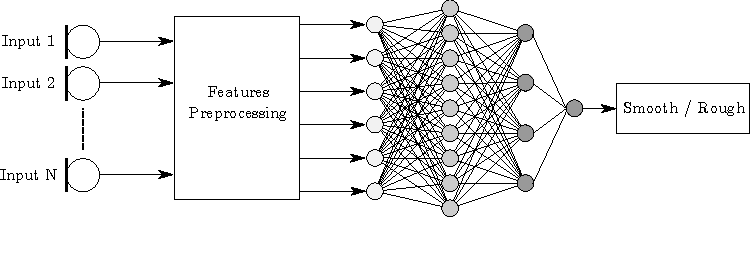
\includegraphics[width=1.0\linewidth]{img/flowchart_1.pdf}
	\caption{Algorithm Block Diagram}
	\label{fig:algoritmo-orizzontale}
\end{figure}


For the road surface classification task we propose an approach based on feature extraction, preprocessing and a classification stage based on a convolutional neural network (CNN) \cite{lecun1995convolutional}. The proposed algorithm is depicted in~\figref{fig:algoritmo-orizzontale}. The preprocessing stage works with short audio chunks to detect abrupt changes in the road surface conditions. We use Auditory Spectral Features, that are calculated in the first stage and then arranged in subsequent and non-overlapping chunks of temporal extension equal to one second in the feature extraction stage. The Neural Network stage deals with the classification and processes one block at a time.

\textbf{NDFAB: aggiungere Siamesi}

\subsubsection{Auditory Spectral Features}

Auditory Spectral Features (ASF) are acoustic features extracted from audio samples that have been introduced in \cite{eyben2010universal} and are used also in \cite{abdic2016detecting}. ASF are computed by applying the Short Time Fourier Transform (STFT) using a frame size of 30\,ms and a frame step of 10\,ms. Each STFT provides the power spectrogram which is converted to the mel frequency scale using a filter-bank with 26 triangular filters obtaining the mel spectrograms $M_{30}(n,m)$, where $n$ is the
frame index, and $m$ is the frequency bin index.

To match the human perception of loudness mel spectrograms are transformed to a logarithmic scale, according to:
\begin{equation}
M_{log}^{30}(n,m) = log(M_{30}(n,m) + 1.0).
\end{equation}
This process yields 26 coefficients, while other 26 are obtained by calculating the positive first order differences $D_{30}(n,m)$ from each logmel spectrogram, as follows:
\begin{equation}
D_{30}(n,m)  = M_{log}^{30}(n,m)-M_{log}^{30}(n-1,m),
\end{equation}
for a total of 52 coefficients for frame. The final feature vector is expanded by including the frame energy and its derivative ending up in a total number of 54 coefficients. %The block diagram of the extraction procedure is depicted in \figref{fig:ASF}. 
The features are extracted with an open-source audio analysis toolkit openSMILE v2.3.0 \cite{Eyben13-RDI} ensuring reproducibility.

%\begin{figure}[h]
%	\centering
%	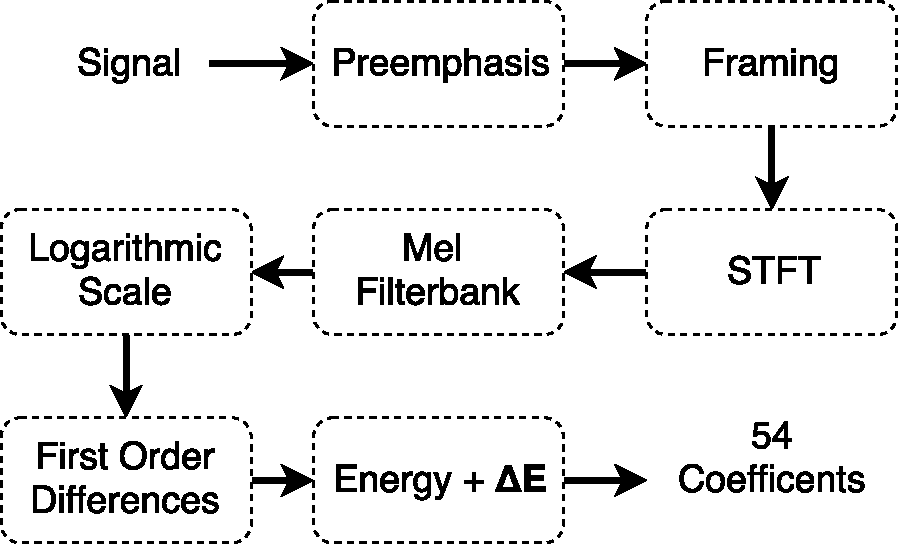
\includegraphics[width=0.5\linewidth]{img/ASF.pdf}
%	\caption{Block diagram of ASF extraction procedure}
%	\label{fig:ASF}
%\end{figure}

In order to feed the CNN, audio chunks of 1\,s are obtained from 98 feature vectors, resulting in 2D arrays of 54-by-98 values.

\subsection{Dataset}

The dataset built for this work is done with a multi-channel microphone arrangement, with the prospect of conducting different assessments at once or to exploit microphone diversity to improve the classification. More specifically, two microphones have been placed close to the rear wheels, one in front of the front left wheel, one inside the engine compartment and two inside the cockpit, close to the driver head and close to the right passenger head. The rear wheel microphones have been placed off-axis, in order to avoid dirt from the wheel and protected by the wheelhouse to reduce the effect of wind. Figure \ref{fig:car-mic} shows the positioning of all microphones. External microphones are \textit{PCB Piezotronics} model 130A24. These are IP55 microphones and they have been protected with a melamine resin foam for sound absorption to reduce the effect of wind. The internal microphones are \textit{PCB Piezotronics} model 378C20. The front-right wheel has been excluded from recordings after first informal evaluations because it picked a large amount of engine noise with respect to the other microphones. The rear-right microphone, vice versa, was found to be the best choice because the noise from the engine was the lowest and it has been used for this first evaluation. The engine compartment microphone has been used to record the engine conditions for future use. In \figref{fig:car-rr-and-fl} are shown the images of the microphones installation. 

\begin{figure}[ht]
	\centering
	\includegraphics[width=0.6\linewidth]{img/car-mic}
	\caption[Car equipment for dataset recording.]{Positioning of the microphones in the car used to record the dataset, top view (a) and bottom view (b). The microphones are placed in the engine compartment (E), close to the front-left, rear-left and rear-right tyres (FL, RL, RR), and inside the car close to the driver or in the back seat (ID, IB). The last two microphones are \textit{PCB Piezotronics} model 378C20 type microphones, while all the others are IP55 \textit{PCB Piezotronics} model 130A24 microphones. The microphones are omnidirectional, however the arrows in (b) show how the capsule was positioned to minimize wind effect. The rear microphones are protected in the wheelhouse.}
	\label{fig:car-mic}
\end{figure}

\begin{figure}[t]
	\centering
	\begin{subfigure}[b]{0.48\textwidth}
		\includegraphics[width=\textwidth]{img/Rear-Right.jpg}
		\subcaption{Rear right tyre microphone.}
	\end{subfigure}
	\hfil
	\begin{subfigure}[b]{0.48\textwidth}
		\includegraphics[width=\textwidth]{img/Front-Left.jpg}
		\subcaption{Front left tyre microphone.}
	\end{subfigure}
	
	
	\caption[Microphones positioning]{Pictures of the \textit{PCB Piezotronics} model 130A24 microphones positioned near the rear right and front left tyres, according to "RR" and "FL" red circles in \figref{fig:car-mic}. The microphones are enclosed by a melamine resin foam with open cell network structure to reduce the wind noise.}
	\label{fig:car-rr-and-fl}
\end{figure}


The car employed to build the dataset is Mercedes A Class from 2014. In addition to the audio signals, the GPS signal has been recorded to track down the car speed and position at any given time. A mobile multi-channel front end, \textit{HEAD Acoustics SQuadriga II}, has been employed as acquisition device, being able to monitor and record 8 contemporary channels at different sample rates, and to store GPS antenna and CAN bus signals as depicted in \figref{fig:car-Squadriga}.
All audio signals are sampled at 44100\,Hz, 24-bits. The external microphones used -26 dBV as input range while the interior microphones had -16 dBV as input range.
To facilitate the labelling operations, a camcorder \textit{BC Master DC10}\footnote{\url{http://www.bc-master.com/product/car-dash-camera-dc10}} was installed on the dashboard of the car. In addition to the video, it provides the speed information obtained through its own GPS antenna and it records the cockpit audio, useful for taking vocal notes while driving.

The data recorded with the \textit{HEAD Acoustics SQuadriga II} have been exported by means of the software \textit{HEAD Acoustics ArtemiS SUITE} in the uncompressed WAV audio format with a 32-bit float representation.

All recordings were taken in dry conditions in the urban and suburban areas of Ancona (Italy) with variable speed, traffic conditions and pavement roughness. Only roads that had been recently asphalted were considered and multiple takes at different speed for each road have been performed. The dataset is not perfectly balanced and is characterized by 41\% of rough road samples and 59\% of smooth road samples. For this reason a balanced version of the dataset, i.e. with equal number of smooth and rough samples, has been created by pruning excess samples for the most populated class. 
The result of the recording sessions is a 50-minutes-long dataset (41 minutes for the balanced version), with 6 audio channels and a speed channel. Labels for the roads have been annotated manually.

\begin{figure}[h]
	\centering
	\includegraphics[width=0.5\linewidth,trim={38cm 18cm 38cm 18cm},clip]{img/Squadriga}
	\caption[HEAD Acoustics SQuadriga II]{Picture of the \textit{HEAD Acoustics SQuadriga II} connected to the GPS-antenna interface.}
	\label{fig:car-Squadriga}
\end{figure}

The spectrograms from two audio samples belonging to the smooth and rough classes are shown in Figure \ref{fig:road_spectrograms}.

\begin{figure}[ht]
	\centering
	\begin{subfigure}[b]{0.48\textwidth}
		\includegraphics[width=\textwidth]{img/specgram_REC007}
		\subcaption{Smooth road.}
	\end{subfigure}
	\hfil
	\begin{subfigure}[b]{0.48\textwidth}
		\includegraphics[width=\textwidth]{img/specgram_REC015}
		\subcaption{Rough road.}
	\end{subfigure}
	\caption[Road noise spectrograms]{Spectrograms from 10 second samples of (a) smooth urban road, (b) rough highway asphalt.}
\label{fig:road_spectrograms}
\end{figure}


\subsection{Evaluation with CNNs}  

\begin{table*}[htbp]
	\footnotesize
	\centering
	\resizebox{\textwidth}{!}{  
	\begin{tabular}{c|c|c|c|c|c}
		Configuration  & Filters        & Kernel Size                            & Strides                              & Max Pooling   & Fully Connected Layers Size      \\
		\hline
		1  & [20, 20]     & $[3\times5], [1\times2]$           & $[3\times3], [1\times2]$          & y, y    & [200, 100] \\
		2  & [15, 20]     & $[3\times5], [1\times2]$           & $[3\times3], [1\times2]$          & y, y    & [200, 100] \\
		3  & [30, 20]     & $[3\times5], [1\times2]$           & $[3\times3], [1\times2]$          & y, y    & [200, 100] \\
		4  & [15, 20, 30] & $[3\times5], [2\times2], [1\times4]$ & $[3\times5], [2\times2], [1\times4]$ & n, y, n & [300, 100] \\
		5  & [20, 20, 30] & $[1\times7], [9\times1], [3\times7]$ & $[1\times7], [1\times9], [2\times2]$ & n, n, n & [300, 100] \\
		6  & [20, 20, 30] & $[1\times7], [9\times1], [3\times7]$ & $[1\times7], [1\times9], [2\times2]$ & n, n, n & [600, 200] \\
		7  & [20, 20, 30] & $[1\times7], [9\times1], [3\times7]$ & $[1\times7], [1\times9], [2\times2]$ & n, n, n & [600, 100] \\
		8  & [54, 54, 30] & $[1\times7], [9\times1], [3\times7]$ & $[1\times7], [1\times9], [2\times2]$ & n, n, n & [200, 100] \\
		9  & [15, 20, 30] & $[3\times3], [2\times2], [1\times4]$ & $[3\times1], [2\times2], [1\times4]$ & n, y, n & [200, 100] \\
		10 & [20, 20, 30] & $[3\times3], [2\times2], [1\times4]$ & $[3\times1], [2\times2], [1\times4]$ & n, y, n & [200, 100] \\
		11 & [20, 20, 30] & $[3\times3], [2\times2], [1\times4]$ & $[3\times1], [2\times2], [1\times4]$ & n, y, n & [300, 100] \\
		12 & [30, 20, 30] & $[3\times3], [2\times2], [1\times4]$ & $[3\times1], [2\times2], [1\times4]$ & n, y, n & [200, 100]
	\end{tabular}
	}
	\caption[Road Surface Roughness Classification - Experiments]{(Best) tested configurations for CNNs. The kernel size and the stride are expressed as $[time\times\,features]$.}
	\label{tbl:config_names}
\end{table*}


Evaluations are reported after a random search of the CNN hyperparameters with different inputs and with both the balanced and unbalanced training sets. A 5-fold cross-validation procedure has been performed. The metrics have been calculated for each combination of training/testing set and then averaged to obtain the unweighted average metrics. The cross-validation has been performed disposing 64\% of the dataset to training, 16\% to validation and 20\% to test. The balanced dataset always performs worse than the unbalanced dataset, suggesting that the pruned information were important for the training stage. After initial tests, the rear-right microphone has been selected being the one with the lowest engine noise content.


In \tableref{tbl:config_names} are reported some of the best configurations tested while in \ref{tbl:cross-valid-res} are shown the best five results obtained. Best performance overall is achieved in the case of the unbalanced dataset with configuration 10, yielding an unweighted average F-measure equal to 86.00\% and an Accuracy of 87.1\%. 
This configuration is composed by three convolutional layers where the first two are square-shaped (2D), thus able to take into account both the temporal evolution and the frequency evolution of the features. The third filter is column-shaped (1D) and is able to take into account the temporal evolution only. Among the tested optimizers, Adam \cite{Kingma2015adam} provided the best results in most of the cases.

Regarding the fully-connected layers, the best results have been achieved using two layers with a number of neurons in the first layer comparable to the number of elements of the feature map obtained from the last convolutional layer. The hyperparameter search showed that oversizing the number of layers or the number of filters/neurons per layer degrades the performance.

\begin{table*}[htbp]
	\centering
	\resizebox{\textwidth}{!}{ 
		\begin{tabular}{c|cccccc}
			Configuration & Batch Size & Accuracy (\%) & F-measure (\%) & Recall (\%) & Precision (\%) & Optimizer \\ \hline
			10       & 5     & 87.10         & 86.00          & 93.08       & 79.92          & adam      \\
			5        & 5     & 86.11         & 85.19          & 93.83       & 78.00          & adam      \\
			2        & 5     & 86.18         & 85.19          & 93.38       & 78.31          & adam      \\
			1        & 1     & 85.88         & 84.87          & 93.41       & 77.76          & adam      \\
			7        & 5     & 85.28         & 83.85          & 89.04       & 79.24          & adam     
		\end{tabular}
	}
	\caption[Road Surface Roughness Classification - Results]{Top 5 configurations sorted by performance obtained in cross-validation analysis with unbalanced training classes. The configuration numbers are the same reported in Table \ref{tbl:config_names}.}
	\label{tbl:cross-valid-res}
\end{table*}


\subsection{Evaluation with Siamese Neural Networks}  

\subsection{Conclusions} 

In the present work a data-driven approach for road surface roughness classification is discussed, following seminal works proposed in the last years. The approach is based on a machine listening approach, where the tyre-road noise is analyzed and classified by means of deep neural networks. With respect to previous works a less computational-intensive neural network architecture has been chosen which also allows for on-line processing. A dataset has been created from a real-world scenario by fitting a car microphones and a GPS receiver and driving the car on different roads with varying speed, gathering a multi-channel dataset of 50 minutes. The CNN has been trained and a hyperparameter search has been done, yielding an F-measure of 86.00\% and an Accuracy of 87.1\% after a 5-fold cross-validation. These results are motivating, however there is headroom for improvement. Specifically, the average precision is lower than the average recall (79.92\% and 93.08\%, respectively), suggesting that some strategy to reduce the number of false positives is required. Unfortunately, given the very different size and complexity of the dataset, results are not comparable with previous works at the moment.

Future works may extend the proposed algorithm to process multiple microphone signals, exploiting diversity, thus reducing the number of errors due to cars passing by and other unrelated sound sources. Driving speed, extracted from a GPS receiver or from the CAN bus, may help improve the classification performance. The most challenging objective, however, would be to infer the road roughness from internal microphones, as these are nowadays available in many vehicles for echo cancellation and noise suppression and are not subject to issues such as dirt, wet, cold, etc. The main issues with this approach, however, are the cockpit isolation from the outside and the interference of speech and music with the road surface noise. Voice activity detection (VAD) \cite{Ephraim:1984,ghosh2011robust} algorithms should be employed and extended to detect the presence of music provided by the car infotainment system. Existing works based on CNN architectures \cite{wirn2016-vad,ijcnn2016-vad} could be a starting point as they could be integrated easily with the current framework and extended.


%\subsection*{Acknowledgments}
%The authors would like to thank ASK industries S.P.A. for financial support and technical assistance.
%This work is supported by the Italian Ministry of Economic Development (MISE)'s fund for the sustainable growth (F.C.S.) under grant agreement (CUP) B48I15000130008, project VASM (“Vehicle Active Sound Management”).
%
%We gratefully acknowledge the support of NVIDIA Corporation with the donation of the GPU used for this research.

%%%%%%%%%%%%%%%%%%%%%%%%%%%%%%%%%%%%%%%%%%%%%%%%%%%%%%%%%%%%%%%%%%%%%%%%%%%%%%%%%%%%%%

\section{Bird Audio Detection}


Automatic wildlife monitoring is a key concern nowadays. Climatic changes, the effects of pollution and alteration of the ecosystems have to be closely controlled in order to be the litmus test for the future sustainable technological and political guidelines.
In this context, bird audio analysis is an important task of the bioacoustics for wildlife and biodiversity monitoring, which can easily embrace the deep learning concept.
In particular, detecting the presence of bird calls in audio recordings is a very common required first step for a framework that can perform different kind of  analysis (e.g. species classification, counting), and makes it possible to conduct work with large datasets (e.g. continuous 24h monitoring) by segmenting the data stream into regions of interests.
To encourage the research in automating this task, in 2016 Stowell et al. \cite{stowell2016bird} organized a first edition Bird Audio Detection (BAD) challenge. It has been appreciated to such an extent that a new round has been included in one of the tasks of the 2018 IEEE AASP Challenge on Detection and Classification of Acoustic Scenes and Events (DCASE). In fact, Task 3 consists in determining a binary decision for the presence/absence of bird sounds on audio files recorded in very different conditions, comprehending dataset balancing, birds species, background sounds and recordings equipment.
Specifically, participants are asked to build algorithms that predict whether a given 10-second recording contains any type of bird vocalization, regardless of the species. Thus, differently from the official name of the task, we can consider it as a \textit{classification} problem.
The organizers invite to explore approaches that can either inherently generalize across different conditions (including conditions not seen in the training data), or which can self-adapt to new datasets. The deep neural network based approach we propose has the aim to counteract the generalization problem by means of an innovative learning procedure named ``capsule routing'' which has shown promising performances since it has been presented \cite{sabour2017dynamic} and also in pioneering employments in audio tasks \cite{iqbal2018capsule}.


\subsection{Related Works}

In very recent years, a strong growth of deep learning algorithms devoted to the acoustic monitoring has been observed. In particular, works such as \cite{mcloughlin2015low, piczak2015environmental, salamon2017deep} represent milestones, involving Convolutional Neural Networks (CNN) for audio signals detection and classification.
These deep neural architectures, combined with the increased availability of datasets and computational resources, have allowed large performance improvements, outperforming in most of the cases the human accuracy \cite{sailor2017unsupervised}. This has also motivated researchers to employ such architecture, eventually combined with recurrent units \cite{cakir2017convolutional}, in almost all of the tasks proposed in the recent editions of research challenges such as the DCASE \cite{DCASE2017challenge}. These algorithms often result among the strongest-performing systems \cite{limrare, valenti2017convolutional}.
Similar results came from the first edition Bird Audio Detection (BAD2017) challenge, which was held in 2016-2017. In this case different novel algorithms have been proposed to create robust and scalable systems able to automate the annotation process of audio sequences containing free-field recordings. The work of Grill and Schl\"{u}ter \cite{grill2017two} should be also mentioned, which obtained the highest score and which is based on CNNs trained on Mel-scaled log-magnitude spectrograms. The outcomes of the BAD2017 are reported in \cite{stowell2018automatic}.

A team at Google Brain recently has presented a new computational unit \cite{sabour2017dynamic} called ``CapsNet'' with the intent to overcome two known limitations of the CNNs: the excessive information loss caused by the pooling and other down-scaling operations and the inability to infer part-whole relationships between the elements which the deep neural network (DNN) has to detect. In fact, the layers of a standard CNN are good at detecting space-invariant features which characterize an image (or a spectrogram in the case of audio spectrograms), but are less effective at exploring the spatial relationships among features (perspective, size, orientation). Capsule routing has the aim to learn global coherence implicitly, thereby improving generalization performance. In the BAD application, it means that the DNN is driven to learn a general concept of the entities of ``bird song'' and ``background sounds'' without requiring extensive data augmentation or dedicated domain adaptation procedures, thus motivating the use of Capsules for this task. 

\subsection{Proposed Method}
The proposed system is a fully data-driven approach based on the CapsNet deep neural architecture presented by Sabour et al. \cite{sabour2017dynamic}.
The novel computational structure of the Capsules, combined to the routing mechanism allows to be invariant to intra-class affine transformations and to identify part-whole relationships between data features.
The whole system is composed of a feature extraction stage and a detection stage. The feature extraction stage transforms time-varying audio signal into acoustic spectral features, then the second stage takes the feature vector as input and maps them to a binary estimate of bird song presence.
This latter stage is where we introduce the Capsule neural network architecture.
The network parameters are obtained by supervised learning using annotations of bird song activity as one hot target vector.

\subsubsection{Feature Extraction}

The feature extraction stage operates on mono audio signals sampled at 44.1 kHz. For our purpose, we exploit \textit{LogMels} as acoustic spectral representation, following results obtained in various audio tagging and sound event detection tasks. Firstly, the audio signals are down-sampled to 16 kHz, because the most relevant frequency bands related to bird songs are in the range from 2 kHz to 8 kHz \cite{payne2010handbook}. Then, \textit{LogMel} coefficients are obtained by filtering the magnitude spectrum of the STFT with a filter-bank composed of 40 filters evenly spaced in the mel frequency scale. The logarithm of the energy of each band is computed to match the human perception of loudness. In the STFT computation, the used frame size is equal to 40 ms and the frame step is equal to 20 ms. 
All of the datasets contain 10-second-long WAV files, thus the resulting feature matrix $\mathbf{x} \in \mathbb{R}^{D_1\times D_2}$ has a shape $501\times40$.
The range of feature values is then normalized according to the mean and the standard deviation computed on the training sets of the neural networks.

\subsubsection{CapNet for Bird Audio Detection}
The architecture of the neural network is shown in Fig. \ref{fig:flowchart}. The first stages of the model are traditional CNN blocks which act as feature extractors on the input \textit{LogMel} coefficients.
After each block, max-pooling is used to halve the dimensions. The feature maps obtained by the CNN layers are then fed to the Primary Capsule Layer that represents the lowest level of multi-dimensional entities. Basically it is a convolutional layer whose output is reshaped and squashed using \eqref{eq:squashing}. The final layer, is a capsule layer and it is composed of two densely connected capsule units.
Since the previous layer is also a capsule layer, the dynamic routing algorithm is used to compute the output. The model predictions are obtained computing the the Euclidean length of each
output capsule, which represent the probabilities that an input feature vector $\mathbf{x}$ belongs to the background or the bird audio class, thus we consider only the latter as system output prediction.

\begin{figure}[htbp]
	\centering
	\includegraphics[width=0.6\columnwidth]{img/capsule_for_bad}
	\label{fig:flowchart}
	\caption[CapsNet for Bird Audio Detection]{Flow chart of the proposed algorithm employing CapsNets for Bird Audio Detection.}
\end{figure}

\subsection{Experimental Set-Up}
\label{sec:experiment}

The network hyperparameters optimization was obtained by means of a \textit{random search} strategy  \cite{bergstra2012random}.  The number and the shape of convolutional layers, the non-linear activation function, the regularizers in addition to the capsules dimensions and the maximum number of routing iterations have been varied for a total of 100 configurations. Details of searched hyperparameters and their ranges are reported in Table \ref{tbl:hyper-params-capsule}.
The neural networks training was accomplished by the AdaDelta stochastic gradient-based optimisation algorithm \cite{zeiler2012adadelta} for a maximum of 100 epochs and batch size equal to 20 on the margin loss function. The optimizer hyperparameters were set according to \cite{zeiler2012adadelta} (i.e., initial learning rate $lr=1.0$, $\rho=0.95$, $\epsilon=10^{-6}$). It was chosen because it is well-suited for dealing with sparse data and its robustness to different choices of model hyperparameters. Furthermore no manual tuning of learning rate is required.

An early stopping strategy was employed in order to avoid overfitting. Thus if the validation score does not increase for 20 consecutive epochs, the training is stopped and the last saved model is selected as the final model. In addition, dropout and L2 (with $\lambda=0.01$) have been used as weights regularization techniques \cite{srivastava2014dropout}. 
The algorithm has been implemented in the Python language using Keras \cite{chollet2015keras} and Tensorflow \cite{tensorflow2015-whitepaper} as deep learning libraries.


\subsubsection{Dataset}
\label{ssec:dataset}
According to the DCASE 2018 guidelines, the performance of the proposed algorithm has been assessed firstly by using the development dataset for training and validation of the system. Then, a blind test on the provided evaluation dataset was performed with the models which achieved the highest performance and submitted to the organizers of the challenge. The complete dataset is composed of recordings belonging to five different collections.  

\begin{itemize}
	\item ``freefield1010'': a collection of 7690 excerpts from field recordings around the world;
	\item ``warblrb10k'': a crowsourced dataset recorded with the \textit{Warblr}\footnote{https://www.warblr.co.uk/} smartphone app. It covers a wide distribution of UK locations and environments and includes weather noise, traffic noise, human speech and even human bird imitations; 8000 samples are used in the development dataset while a held-out set of 2,000 recordings from the same conditions is included in the evaluation split;
	\item ``BirdVox-DCASE-20k'': 20000 files containing remote monitoring flight calls collected from  recordings units placed near Ithaca, NY, USA during the autumn of 2015;
	\item ``Chernobyl'': dataset collected from unattended remote monitoring equipment in the Chernobyl Exclusion Zone (CEZ). A totoal of 6620 audio files cover a range of birds and includes weather, large mammal and insect noise sampled across various CEZ environments, including abandoned village, grassland and forest areas;
	\item ``PolandNFC'': 4000 recordings obtained from a project of monitoring of autumn nocturnal bird migration. They were collected every night, from September to November 2016 on the Baltic Sea coast, Poland, using Song Meter SM2 units with microphones mounted on 3–5 m poles.
\end{itemize}
Further details are reported in Table \ref{tab:dataset}.
The organizers recommended a 3-way cross-validation (CV) for the algorithms development, thus in each fold we used two sets for training and the other one as validation set in order to have scores comparable with the others challenge participant.

\begin{table}[t]
	\centering
	\begin{tabular}{|c|c|c|}
		\hline
		\ \textbf{Collection} \rule{0pt}{10pt} & \textbf{N. of samples}  & \textbf{Balance} \\
		\hline
		\hline	
		\multicolumn{3}{|c|}{\textbf{Development Dataset}  \rule{0pt}{10pt}} \\ 
		\hline
		``warblrb10k'' & 8000 & 0.75 \\
		\hline
		``BirdVox-DCASE-20k'' & 20000 & 0.5 \\
		\hline
		``freefield1010'' & 7690 & 0.25 \\
		\hline
		
		Total 	& 35690	& 0.5 \\
		
		\hline
		\hline
		
		\multicolumn{3}{|c|}{\textbf{Evaluation Dataset}  \rule{0pt}{10pt}} \\ 
		\hline
		``warblrb10k\_test'' & 2000 & - \\
		\hline
		``Chernobyl'' & 6620 & - \\
		\hline
		``PolandNFC'' & 4000 & - \\
		\hline
		Total 	& 12620 & - \\
		\hline
	\end{tabular}
	\caption[Bird Audio Detection - DCASE 2018 dataset]{Details of the dataset we used for the algorithm development. The table shows the number of audio files and the ratio between positive/negative samples (if available) of each used data collection.}
	\label{tab:dataset} 
\end{table}


\begin{table*}[h]
	\centering
	\small
	\resizebox{\textwidth}{!}{
	\begin{tabular} {|c | c | c| c | c | c |}
		\hline
		Parameter & Range & Distribution & CapsNet1 & CapsNet 2 & CapsNet3\\  
		\hline
		\hline                                     
		CNN layers Nr.  & [1 - 4]& uniform & 3 & 4  &  4  \\
		\hline                                     
		CNN kernels Nr. & [4 - 64]& log-uniform & [64,16,8]  & [32,16,16,32] & [32,64,4,64] \\
		\hline    
		CNN kernels dim. & [3$\times$3 - 8$\times$8]& uniform & 3$\times$3 & 5$\times$5 & 6$\times$6 \\
		\hline   
		\multirow{2}{*}{Pooling dim.} & \multirow{2}{*}{[1$\times$1 - 2$\times$5]}& \multirow{2}{*}{uniform} & [1$\times$5],[1$\times$4], & [1$\times$5],[1$\times$4], &  [1$\times$4],[1$\times$2], \\
		&											  &							   & [1$\times$4]				& [1$\times$2],[1$\times$2]	&	[1$\times$2],[1$\times$2] 	\\
		\hline                                   
		CNN activation & [tanh - relu] & random choice & tanh & relu &  relu \\
		\hline
		CNN dropout  & [0 - 0.5]	& uniform & 0 & 0 & 0 \\
		\hline
		CNN L2  & [yes - no]	& random choice & no & yes & yes \\
		\hline
		\hline
		Primary Capsules channels Nr. & [2 - 8]	& uniform & 6 & 2 & 8  \\
		\hline   
		Primary Capsules kernels dim. & [3$\times$3 - 5$\times$5]& uniform & 4$\times$4 & 4$\times$4  &  3$\times$3 \\
		\hline  
		Primary Capsules dimension & [2 - 16]	& uniform & 8 & 8 & 2 \\
		\hline  
		Capsules dimension & [2 - 16]	& uniform & 2 & 15  & 10 \\
		\hline
		Capsules dropout  & [0 - 0.5]	& uniform & 0 & 0.1 & 0.3 \\
		\hline
		Max routing iterations  & [1 - 5]	& uniform & 2 & 3 & 2 \\
		\hline
		Batch Normalization  & [yes - no]	& random choice & yes &  yes  &  yes  \\
		\hline
		\hline
		Trainable Params & - & - & 113k & 282k & 424k \\
		\hline
	\end{tabular}
	}
	\caption[CapsNet for Bird Audio Detection - Experiments]{Hyper-parameters optimized in the random-search phase and the resulting best performing models.}
	\label{tbl:hyper-params-capsule}
\end{table*}



\subsubsection{Baseline}
The baseline system is an adapted version of the method winner of the BAD2017 \cite{grill2017two}. The peculiarity of this algorithm is its double training procedure. In a first run, the network is trained on the whole training data. Binary predictions are obtained for the testing data. The more confident predictions (the ones closer to 0 or 1) are then added to the training data as so-called ``pseudo-labeled'' samples. Thus, a second training run is performed on this extended training set and the final predictions are yielded.


\subsubsection{Metric}
The performance metric of the DCASE 2018 on this task is the ``Area Under the ROC Curve'' (AUC). More precisely, it is a stratified AUC: the score is computed separately for each fold of the evaluation set, then the partial scores are averaged. This procedure allows to adapt the ``detection threshold'' to each dataset conditions, then the performance across datasets are combined in an explicit weighted fashion, thus the final score is not merely influenced by the number of files in each subset.


\subsection{Results}
\label{sec:results}
\subsubsection{Results on Development dataset}
Results reported in Table \ref{tab:results} show both the best performance we obtained on the single CV fold, and the best averaged AUC. We obtain a harmonic mean for AUC equal to 83.72 for a single configuration, whilst if we consider the mean of the best performing models on the single folds we achieve an AUC equal to 85.08.


%\subsubsection{Preview Score on Evaluation dataset}
%We considered as candidates for the test on the evaluation procedure \cite{dcase2018web} both the best performing setups on the single CV folds (submission label \textbf{Vesperini\_UnivPM\_task3\_1}), and the setups with the best averaged AUC (submission label \textbf{Vesperini\_UnivPM\_task3\_2}). For the latter, we trained a new model with the same hyperparameters on the whole development dataset before performing the predictions on the evaluation dataset.
%
%
%The DCASE 2018 featured a submission site where contestants could upload their predictions and compute a ``preview score'' for a subset of around 1000 files from the test set. With an ensemble of the single fold best models trained during the CV procedure we obtain an AUC score equal to 84.43, while for the model with the best averaged AUC we obtain an AUC score equal to 81.43.


\begin{table}[t]
	\centering
	\begin{tabular}{|l|c|c|c|c|c|}
		\hline
		Conf ID & Fold 1 & Fold 2	& Fold 3 & Avg & Preview Score \\
		\hline
		Baseline &	-	&	-		&	-	& 83.00 &  89.18		\\
		\hline
		CapNet1	&  \textbf{88.22} & 72.78	& 74.16	& 78.39 & -	\\
		CapNet2	&  81.77 &  \textbf{80.90} 	& 85.52	& 82.73	& 	- \\
		CapNet3	&  86.59 & 78.46	&  \textbf{86.11}	&  83.72 				& 81.83  \\
		Ensemble &	-	 & 		-	&		-			&		\textbf{85.08}  & \textbf{84.43} \\
		\hline		
	\end{tabular}
	\caption[CapsNet for Bird Audio Detection - Results]{Results on Development dataset in terms of AUC (\%).}
	\label{tab:results}
\end{table}


\subsection{Conclusion and Outlook}
\label{sec:conclusion}

In this work, we have presented an algorithm for bird audio detection based on the CapsNet architecture. We feed a deep neural network which uses the dynamic routing procedure during the training with the \textit{LogMel} extracted from the audio signals in order to obtain predictions on unseen data recorded in various conditions possibly also very different from the training set. 
To assess the performance of the algorithm we conducted experiments on the development dataset from the DCASE 2018, obtaining an AUC score equal to 85.08 with respect to an AUC equal to 83.00 of the baseline system.
For future work, variants \cite{hinton2018matrix} or strategy to customize the dynamic routing can be considered.



\graphicspath{{5_sound_event_detection/}}
\chapter{Sound Event Detection}
\label{ch:SED}

The task of sound event detection (SED) is defined as the task of analysing a continuous audio stream in order to extract a description of the sound events occurring in it. This description is commonly expressed as a label that marks the start, the ending, and the nature of the occurred sound (e.g., children crying, cutlery, glass jingling). In this chapter three related works are shown, which are respectively: Overnight Snore Sounds Detection by means of Convolutional Recurrent Neural Networks (CRNN) and acoustic data augmentation; Convolutional Neural Networks with 3-D Kernels for Voice Activity Detection in a Multiroom Environment; and Rare Sound Detection, consisting in detection of three sound categories (i.e., gunshot, babycry and glassbreak) from a highly imbalanced dataset. The latter has been performed by means of a hierarchical framework of ConvNets.

\section{Overnight Snore Sounds Detection}
\label{sec:snoring_detection}
As described in \secref{sec:snoring_classification}, one of the most common sleep disorder is the chronic snoring. In the occasion of the Interspeech 2017 ComParE challenge \cite{ComParE2017} and subsequent investigations, different approaches based on Deep Neural Networks (DNNs) have been presented \cite{amiriparian2017snore}, \cite{freitag2017end}, \cite{vesperini2018snore} with the aim to classify isolated snore sound events among the four classes based of the VOTE scheme.

In this work, we propose the application of Convolutional Recurrent Neural Networks (CRNNs) to detect snoring episodes from overnight recordings acquired in real life conditions. The method is a two step process: the acoustic spectral features extraction and the CRNN combined with Gated Recurrent Units (GRU) processing. The algorithm is evaluated by using the Average Precision (AP) score.
Differently from other deep learning approaches \cite{amiriparian2017snore}, \cite{freitag2017end}, \cite{vesperini2018snore}, this choice offers a viable and natural solution for jointly learning the spatio-temporal dependencies of audio sequence for discovering snoring event. Additionally, we deal with the high unbalanced setting which exists in the task of snore detection. The original snore/background ratio in the aforementioned signals has been increased by adding isolated snore events from the Munich-Passau Snore Sound Corpus dataset \cite{ComParE2017} (cf. \secref{ssection:MPSSCdataset}). The reliability of the proposed approach is investigated using the A3-snore dataset, leading to significant improvement in term of Average Precision (AP) with respect to Convolutional Neural Network (up to 9.48\%) and other data augmentation techniques.


\subsection{Proposed Approach}

The two step of the proposed approach are detailed in this section, starting from the spectral features extraction and ending with the Convolutional Recurrent Neural Network.

\begin{figure}[t]
	\centering
	\includegraphics[width=0.9\columnwidth]{img/snore_detection_4.pdf}
	\caption[Snoring Detection with CRNNs]{The proposed approach scheme for Snoring Detection.}
	\label{fig:overall}
\end{figure}

\subsubsection{Features Extraction}
The feature extraction stage operates on stereo audio signals sampled at 44.1 kHz. 
Following the results obtained in recent works related to sound event detection \cite{DCASE2017Workshop}, we use the log Mel energy coefficients (Logmel) as an efficient representation of the audio signal. The stereo signal is firstly down-mixed to mono by averaging the two channels. 
The resulting audio signal is split into 30\,ms frames and a frame step of 10\,ms to compute the STFT spectrogram. We used a filter bank with 40 mel scaled channels, obtaining 40 coefficients/frame. 

\subsubsection{Convolutional Recurrent Neural Networks}


CRNNs used in this work are composed of four types of layers: convolutional layers, pooling layers, recurrent layers and detection layer. 
Each convolutional layer is followed by batch normalization per feature map \cite{ioffe2015batch}, a leaky rectified linear unit activation function (LeakyReLU) and a dropout layer \cite{srivastava2014dropout} with rate equal to $0.3$.
A frequency domain max-pooling layer is then applied to the resulting feature-map, in order to enhance the relevant information from frequency bands without lose the temporal resolution of the Logmels, as proposed in \cite{cakirconvolutional}. The extracted features over the CNN feature maps are stacked along the frequency axis. Max-Pooling operation combined with shared weight in convolutional layers provide robustness to frequency shifts in the input features and this is crucial to overcome the problem of intra-class acoustic variability for snore events.
In the recurrent block, the stacked features resulting from the last pooling layer are fed to layers composed of GRUs (cf. \secref{sssec:GRU}), where tanh and hard sigmoid activation functions are used for update and reset gates, respectively.
Fast response to the changes in the input and the previous activation information is fundamental for high performance in the proposed algorithm, where the task is to detect a small chunk of consecutive time frames where the target event is present. In addition, a previous work \cite{valenti2017neural} demonstrates improvements provided by recurrent architectures in the sound event detection in real-life audio.
The detection layer is a feed-forward layer of composed of a single neuron with sigmoid activation function, corresponding to the probability the event onset. The layer is time distributed, this means that while computing the output of the classification layer, the same weight and bias values are used over the recurrent layer outputs for each frame.

In a comparative aim, we implemented also a CNN architecture very similar to the CRNN, the only difference being that the recurrent layers of the CRNN are replaced with time distributed feed-forward layers with ReLU activations. In following section, we will refer it as CNN.


The neural networks training was accomplished by the AdaDelta stochastic gradient based optimisation algorithm \cite{zeiler2012adadelta} for a maximum of 500 epochs on the binary cross entropy loss function. The optimizer hyperparameters were set according to \cite{zeiler2012adadelta} (i.e., initial learning rate $lr=1.0$, $\rho=0.95$, $\epsilon=10^{-6}$). An early stopping strategy, monitoring the validation AP score, was employed in order to reduce the computational burden and avoid overfitting. 


\subsection{A3 Snore Dataset} 

The snore detection algorithm has been evaluated on the A3-Snore dataset. A brief description of the acquisition setup and dataset splitting is provided in the following.

\subsubsection{Acquisition setup:}
In order to capture the overnight audio recordings a ZOOM-H1 Handy Recorder has been used. It is equipped with two unidirectional microphones set at a 90 degree angle relative to one another. The signals are stored in WAV files with a sampling rate of 44.1\ kHz and bit depth equal to 16.
The input gain is automatically set by the recorder to prevent overload and distortion, while the high-pass filter was enabled in order to eliminate pops, wind noise, blowing, and other kinds of low frequency rumble.


\subsubsection{Acquisition environment:}
The acquisition environment consist of a simple bedroom, with two access points (door and window). The recorder is placed near the patient, at same height of the bed and in line with the subject's mouth. During the recordings, the patient is the only one that can occupy the bedroom, in order to avoid contaminations on recorded audio signals. The room dimensions are reported in \figref{fig:room}.
Background sounds include traffic noise, breathing and speech signals, house and animal noises. We acquired some samples measurements of the event-to-background (EBR) ratios considering background noise, snoring events and noise events such as ``car passing by'' or ``dog barfing''. The EBR resulted equal to 6.5 dB and 1.1 dB respectively for noise to background EBR and snore to background EBR. 


\begin{figure}[t]
	\centering
	\includegraphics[width=0.6\columnwidth]{img/room.pdf}
	\caption[Recording Room]{Plant of the recording room.} 
	\label{fig:room}
\end{figure}


\subsubsection{Dataset splitting:}
The original recordings have been manually labelled, annotating the snore events onset and offset with a resolution of 1 second. The audio sequences have been divided into chunks of 10 minutes, and only those with the highest number of snore events have been used in the experiments. 
The dataset is organized into subjects, which can be respectively used as \emph{training} or \emph{validation} sets in a two fold cross validation strategy (i.e., Leave One Subject Out procedure). The number of events per class in the database is strongly unbalanced as reported in \tableref{a3snore}. Thus, the snore detection task is challenging, due to the high number of noises on the A3-SNORE dataset. 

\begin{table}[ht]
	\centering
	\resizebox{\textwidth}{!}{
	\begin{tabular}{cccccc}
		\hline
		\multicolumn{6}{c}{\textbf{A3-SNORE dataset}} \\
		\hline
		\# & Gender & Age & Snoring (SN) & Total Duration (Tot) & Ratio (SN/Tot) \\
		\hline
		Snorer 1 & M & 48 & 33m-27s & 3h-12m-0s & 14.5\% \\
		Snorer 2 & M & 55 & 21m-21s & 3h-50m-0s & 11.1\% \\
		\hline
		\multicolumn{3}{l}{Total} &	54m-48s	& 7h-02m-0s	& 12.8\%\\
		\hline    
	\end{tabular}
	}	
	\caption[A3-SNORE dataset]{Difference of recording times for each class, divided by snorers.}
	\label{a3snore} 
\end{table}

\subsection{Data Augmentation Techniques}
\label{ssec:data-augmentation}
In this application, what we are really interested is to detect the minority class (e.g. snoring events) rather than the majority class (e.g. background). Thus, we need to adequately train the models in order to obtain a fairly high prediction for the minority class. In order to counteract the dataset unbalancing existing in the task of snoring detection different techniques of data augmentation have been evaluated. 
The literature suggests that it is possible to augment training data in data-space or in feature-space. 
In this work, both data augmentation approach have been evaluated, by using the \emph{Synthetic Minority Over-sampling Technique} (SMOTE) \cite{chawla2002smote} in the feature space, and by generating simulated data with an increased number of snore events. 
The original snore/background ratio in the acquired signals has been increased with these transformations to approximately 30\% \cite{young1997nasal}, maintaining anyway a natural unbalance which is properly of this task.
In the following sub-sections, a brief description of each method is provided.

\subsubsection{Majority Class under sampling:} it is not a properly data augmentation technique but it is a fast and easy way to balance the data. It consists in randomly selecting a subset of data from the training sets in order to modify the ratio of the sample occurrences in two classes.

\subsubsection{SMOTE:} It is an over-sampling approach in which the minority class is over-sampled by creating new synthetic examples. The minority class is over-sampled by taking each minority class sample and introducing synthetic examples along the line segments joining any/all of the \emph{k} minority class nearest neighbors (\emph{k}-NN). Depending upon the amount of required over-sampling, neighbors from the \emph{k}-NNs are randomly chosen. In particular, synthetic samples are generated in the following way: the difference between the feature vector (sample) under consideration and its nearest neighbor is multiplied by a random number between $0$ and $1$, and this is added to the feature vector under consideration. In details, for a sample $x_{i}$:
\begin{equation}
x_{j}^{\text{SMOTE}} = x_{i} + (\tilde{x}_{i,k} - x_{i}) \cdot r(j)
\end{equation}
where $r(j) \in [0,1]$.
This causes the selection of a random point along the line segment between two specific features. This approach effectively forces the decision region of the minority class to become more general. 

\subsubsection{Proposed approach - Generating simulated data:} The simulated training sets have been created starting from the folds described in \secref{ssec:dataset}.
The impulse responses between the snore source and the microphones have been recreated by using the library Pyroomacoustics \cite{Scheibler2018}.
Isolated snore sounds have been taken from the Munich-Passau Snore Sound Corpus (MPSSC) dataset \cite{ComParE2017}. It is composed of 843 snore events which have been extracted and manually screened by medical experts from Drug-Induced Sleep Endoscopy (DISE) examinations of 224 subjects.
The augmented training set has been created by convolving the isolated snore sound events of the MPSSC corpus with the synthetic impulse responses. Than, the obtained signals have been mixed with the original recordings without overlap with the already present events. The artificial added event dynamic was normalized to the maximum value observed in the original signals. The resulting total time of snore signals is 55 minutes for Snorer 1, and 56 minutes and 5 seconds for Snorer 2.

\subsection{Experimental Setup}
The performance of the algorithms has been evaluated in term of AP score, a metric that summarizes the Precision and Recall curve (cf. \secref{sec:evaluation_metrics}).
To asses the performance of the models, we explored different hyper-parameter configurations and, for each of these, we repeated the whole experiments training the models both with the original data and  with  data processed with techniques described in \secref{ssec:data-augmentation}. \tableref{CNN-params} shows the hyper-parameter configurations analyzed in our experiments. They regard kernels size, kernel number and GRUs for a total of 120 experiments. In the case of CNN the number of units and layer refers to a Multi Layer Perceptron (MLP) architecture. The experiments were conducted in a 2-fold cross-validation strategy corresponding on a leave one subject out procedure, thus in fold 1 we used Snorer 1 as training set and Snorer 2 as validation set and in fold 2 vice-versa. The models were selected on the performance based on the AP score  averaged on the two folds. 
The algorithm has been implemented in the Python language using Keras \cite{chollet2015keras} as deep learning library. All the experiments were performed on a computer equipped with a 6-core Intel i7, 32\,GB of RAM and two Nvidia Titan X graphic cards. 

\begin{table}[ht]
	\centering
	\begin{tabular}{|l|r|}
		%		\hline
		%		\multicolumn{2}{|c|}{Network Layout Parameters}            \\ \hline
		\hline
		Convolutional Layers Number & 3                            \\ \hline
		Kernel Number               & 4, 8, 16, 32, 64                 \\ \hline
		Kernel Size                 & $5\times5$, $3\times3$, $2\times2$ \\ \hline
		Pooling Size                & $5\times1$, $4\times1$, $2\times1$ \\ \hline
		\hline
		Recurrent Layers Number     & 2, 3                            \\ \hline
		Dense Layers Number     & 2, 3                            \\ \hline
		Number Of Units             & 4, 8, 16, 32, 64                 \\ \hline
	\end{tabular}
	\caption[Snoring Detection - Experiments]{Explored network layout parameters.}
	\label{CNN-params}
\end{table}


\subsection{Results}
The performance of the CRNN and CNN architectures using different data augmentation techniques are reported in \figref{fig:results}. In blue are depicted results with CRNN, in green the results of the CNNs. The CRNNs show to be effective for snore event detection yet with the original data, although the dataset imbalance. The best performing model is composed of 3 CNN layers with respectively [64,64,64] filters of size $3\times3$ and two GRU layers of 64 units. This configuration obtains an AP up to 82.05\%, with a difference of +7.79\% with respect to the CNN.

\begin{figure}[h]
	\centering
	\includegraphics[width=0.7\columnwidth]{img/grafTex/results.pdf}
	\caption[Snoring Detection - Results]{Results with different data augmentation techniques for the best models of the evaluated architectures.} 
	\label{fig:results}
\end{figure}

The majority class under-sampling and the SMOTE techniques obtain worst performance with respect to original recordings. For majority class under sampling this can be motived by the necessity of DNN models of a large amount of data to be trained properly, thus a reduction of data samples cannot benefits to their detection ability. Regarding the SMOTE, the performance reduction is less dramatic (-0.16\% and -0.08\%, respectively, for CNNs and CRNNs) but its employment remains vain. In this case, the motivation can be found on the complexity to generate new samples of audio signals in the feature space which can really improve a DNN perfomance.

The addition of isolated snore samples convolved with the simulated room impulse response has a tangible beneficial effect on the examined models. In fact, with this technique we obtain an AP improvement equal to 11.18\% and 12.87\%, respectively, for the CNN and the CRNN. The latter obtains an AP equal to 94.92\% with an architecture composed of 3 CNN layers with respectively [64,32,32] filters of size $5\times5$ and two GRU layers of 32 units.
This model is composed of 91,553 free-parameters and occupies approximately 1.2 MB, providing to the algorithm a feasible complexity in an application scenario.


\subsection{Conclusion}
In this work, a deep learning algorithm based on a CRNN architecture fed with Logmel spectral features extracted from the audio signal has been proposed for snore detection. The A3-Snore dataset has been acquired in real-world conditions, containing overnight recordings of two male subjects and it has been used to assess the performance of the models. The original snore/background ratio has been increased by adding isolated snore events from the Munich-Passau Snore Sound Corpus dataset \cite{ComParE2017}. The reliability of the proposed approach has been investigated with respect to baseline CNN and different data augmentation techniques such as oversampling (i.e., SMOTE) and downsampling. Results show that the presented snore detection methodology is able to better generalize across different users. In particular, the CRNN is able to extract salient information from the spectral features in order to discriminate snore events, while the implemented data augmentation provide additional samples of the minority class (i.e., snore events). These samples contains supplementary information that can be exploited by the CRNN for learning and discriminate snore events.
Future works will be addressed to employ this methodology in a weakly supervised setting.
Specifically, in the real-life applications, the precise annotation of existing events from overnight recordings can be onerous and can be result in sparse labeling. Machine learning models trained in a weakly supervised fashion can help to counteract this problem without losing the state of the art performance.

\newpage
%%%%%%%%%%%%%%%%%%%%%%%%%%%%%%%%%%%%%%%%%%%%%%%%%%%%%%%%%%%%%%%%%%%%%%%%%%%%%%%%%%%%%%%%%%%%%%%%%%%%%%%%%%%%%%%%%%%%%%%%%%%%%%%%%%%

\section{Rare Sound Event Detection}
\label{sec:rare_sed}
The ``Detection of rare sound events'' task of the 2017 Detection and Classification of Acoustic Scenes and Events (DCASE) challenge \cite{DCASE2017Workshop} consisted in determining the presence and the precise onset time of three types of sounds, ``baby cry'', ``glass break'' and ``gun shot'' in artificially generated audio sequences. 
The task takes into account real-world issues that introduce additional complexity to the problem, such as the acoustic variability of the sounds belonging to each event class, the presence of environmental noise and its variability, etc. The rules of the challenge allow to know \textit{a priori} the event typology possibly present in the audio sequence under examination, thus it is possible to have a separate binary classifier for each class.

\subsection{Related Works}
In the recent era of the ``Deep Learning'' different approaches to SED have been proposed marking use of the capabilities of deep neural networks (DNNs) to learn the relation between time-frequency features of the raw audio signal and a target vector representing sound events.
Although the DNNs based systems are more computationally intensive with respect to  widely used statistical modelling methods such as hidden Markov models (HMMs) or Gaussian mixture models (GMMs)  \cite{heittola2010audio, peng2009healthcare}, a comparative study \cite{sigtia2016automatic} has highlighted that they are able to achieve top performance in the sound recognition problem.

A well-fitting example of such performance is given in~\cite{marchi2017deep}, where different DNNs are trained on three datasets recorded in real life environments in order to detect abnormal events or hazardous situations exploiting only the information carried by the acoustic signal. The experimental results show that Deep Recurrent Neural Networks (DRNNs) outperform the probabilistic approaches over the three databases. 
Another example focuses on employing Convolutional Neural Networks (CNN)  for Voice Activity Detection in multi-room domestic scenarios (mVAD) \cite{vecchiotti2018convolutional}. The CNN-mVAD results to be effective and outperforms the other method with a significant solidity in terms of performance statistics.

In occasion of the DCASE 2017 challenge, many novel systems featuring deep neural networks have been proposed, in particular involving hybrid architectures making use of Convolutional Neural Networks (CNN) and DRNNs. In detail, both the first two classified algorithms make use of mel spectrogram coefficients as spectral representation of the audio signal which is processed by a CNN with 1D filters in the case of the first ranked \cite{limrare} or by a 2D CNN with frequency pooling in the case of the second classified \cite{cakirconvolutional}. The architectures are, then, combined with recurrent layers to process the features obtained by the convolutional blocks.
In \cite{phan2017dnn} the authors propose a hierarchical structure based on CNNs and DNNs trained with multi-task loss functions. Specifically, in the first stage the networks are trained for background noise rejection, using a weighted loss function to penalize the false positive errors. In the second stage the multi-task loss enables the networks to simultaneously perform the event classification task and the onset time estimation. This approach obtained the third place in the final ranking. 
All of the aforementioned systems largely outperform the baseline system based on a Multi Layer Perceptron architecture (MLP) and Logmel energies as features.
The baseline system \cite{DCASE2017challenge} is based on a Multi Layer Perceptron architecture (MLP) and log mel energies as features. For each audio frame, the input vector is constructed concatenating 5 adjacent log mel vectors for a total of 200 elements. The ANN architecture consists of two dense layers of 50 hidden units each and one output neuron with sigmoid activation, which indicates the activity of the target class.

\subsection{Proposed Method}
The proposed system is a hierarchical algorithm composed of five stages: the acoustic features extraction, the event detection stage 1,  which produces an output at frame-rate and a dedicated smoothing procedure of this signal.
Then, a refinement of the previous decision stage is performed by a 2D CNN which discards possible false positives detected by the stage 1. The final decision procedure annotates the effective onset time of the active event. In \figref{fig:flow-chart-rare-sed} the phases of the algorithm are depicted. This is an extended and improved method with respect to our contribution to the DCASE 2017 \cite{vesperinihierarchic}.

\begin{figure}[t]
	\centering
	\includegraphics[width=0.9\columnwidth]{img/approccio_finale_1.png}
	\caption[Proposed Approach for Rare Sound Event Detection]{Flow chart of the proposed method for rare sound event detection. Each event class implements such a scheme. In the first column are shown the spectrograms of the input signal and of the detected events. In the second column the network outputs at each stage of the algorithm.}
	\label{fig:flow-chart-rare-sed}
\end{figure}

\subsubsection{Features Extraction}
The feature extraction stage operates on mono audio signals sampled at 44.1 kHz. 
Following the results obtained at the DCASE2017 challenge by \cite{cakirconvolutional}, we use the log mel energy coefficients (Logmel) as an efficient representation of the audio signal. In addition, we explored the combination of the Logmel with features based on wavelet coefficients and forward prediction errors (WC-LPE) \cite{marchi2014multi}. A brief description of the features extraction procedures is given below.
\paragraph{Logmel coefficients}
The audio signal is split into frames of 40\,ms and a frame step of 20\,ms, then the Logmel coefficients are obtained by filtering the power spectrogram of the frame as described in \secref{ssec:ac_features}. In this work, we used a filter bank with 40 mel scaled channels, obtaining 40 coefficients/frame. 

\paragraph{WC-LPE Feature}
The Wavelet Coefficient (WC) and Linear Prediction Error (LPE) feature set relies on non-stationary signal components and it has been successfully exploited for musical note onset detection \cite{marchi2014multi}. WC-LPE extraction is done by first processing the input signal with a Discrete Wavelet Transform (DWT) dyadic tree. Then, each DWT sub-band is filtered by a linear prediction error filter (LPEF), obtaining Forward Prediction Errors (FPE). All LPEF outputs and DWT sub-bands are resampled to an intermediate sampling rate and rectified. The feature set is, finally, created from the DWT sub-bands, their first order time derivatives, the FPE and their first order time derivatives.

For both feature sets the range values of each coefficient is normalized independently according to the mean and the standard deviation computed on the training sets of the neural networks.

\subsubsection{Event Detection Stage 1}
The Event detection (ED) stage 1 has the goal to discard frames containing only background sounds, reducing as much as possible the false negative decisions.
We evaluated two DNN architectures as binary classifiers: the MLP and the CNN with 2D kernels and frequency pooling. In both cases, the output layer is formed by two units with the \textit{softmax} non-linear function. Thus, the networks outputs represent the probabilities that an input feature vector $\mathbf{x}[t]$ at the frame index $t$ belongs to the background or the event class. In our analysis, we evaluated as network input the Logmel coefficients and the combination of the latter with the WC-LPE features.

\subsubsection{Deep Neural Network Architectures}
For the ED stage 1 we compared the performance of two deep neural networks architecture, respectively the Multi Layer Perceptron (MLP) and the Convolutional Neural Networks (CNN). In both cases, the neural networks training was accomplished by the AdaDelta stochastic gradient-based optimisation algorithm \cite{zeiler2012adadelta} for a maximum of 500 epochs on the binary cross entropy loss function. The optimizer hyperparameters were set according to \cite{zeiler2012adadelta} (i.e., initial learning rate $lr=1.0$, $\rho=0.95$, $\epsilon=10^{-6}$). An early stopping strategy monitoring the validation loss was employed in order to reduce the computational burden. Thus if the validation loss does not decrease for 20 consecutive epochs, the training is stopped and the last saved model is selected as the final model. In addition, dropout is used as regularization technique \cite{srivastava2014dropout} with rate $0.5$. 

\paragraph{Multi Layer Perceptron Neural Network}
The network is designed to consider a temporal context  $C$, thus the network input  feature vector  $\hat{\mathbf{x}}[t]$ is obtained concatenating $\mathbf{x}[t]$ with the previous $\mathbf{x}[t - c]$, with $c = 1, \dots, C$. 
 
During the training procedure, additive zero-centered Gaussian noise with $\sigma=0.1$ was applied to $\hat{\mathbf{x}}[t]$ as a form of data augmentation, improving the generalization capabilities of the DNN and avoiding overfitting \cite{marchi2017deep}.


\paragraph{Convolutional Neural Network}
\label{ssec:CNN}

In our case the convolutional layer input is a matrix $\mathbf{X} \in \mathbb{R}^{F \times T}$, where $F$ and $T$ represent respectively and the number of Logmel channels and the number of frames of the acoustic signal.
When we combine the two aforementioned feature sets, we process them with two separate sets of convolutional layers, gathering two feature maps that are concatenated along the feature axis. Before concatenation, batch normalization \cite{ioffe2015batch} is applied to each feature map and a leaky rectified linear unit activation function (LeakyReLU) with $\alpha=0.3$, followed by a feature domain max-pooling layer.
Finally, fully connected layers are stacked, applying the same weights and biases to each frame element. The output layer for each of the binary classifier neural networks has two neurons corresponding to the probability of the background or the event onset. We can discard, thus, one of the two neurons without loss of information, and we will consider the output of the neuron corresponding to the event activation $u[t] = y_{t,2}$, as the output of the network at frame $t$.


\subsubsection{Post Processing}
In the post processing stage, each network output is convolved with an exponential decay window of length $M$ defined as:
\begin{equation}
	\mathbf{w}[t]= e^{-\frac{t}{\tau}} \quad \text{with}  \, \tau =  \frac{-(M-1)}{log_e(0.01)}
\end{equation}
The result is processed with a sliding median filter with local window-size $k$. Finally, a decision threshold $\theta$ is applied.

\subsubsection{Event Detection Stage 2}

The aim of the event detection stage 2 is to eliminate false positives, by removing the events wrongly detected at the previous stage. This is done by feeding a binary-classifier CNN with chunks of features in correspondence to the detected events (colored region in the bottom right spectrogram of \figref{fig:flow-chart-rare-sed}). At this stage only Logmel coefficients are used as input features, in order to reduce the computational burden of the model. Non-overlapping feature matrices $\mathbf{X}$ of size $F\times20$ are used during training, while 95\%-overlapping feature matrices are employed during testing (1-frame shift).
A chunk size of 20 corresponds to 0.4 seconds of audio, i.e. half the minimum possible length of the occurring events, leading to an analysis of the audio event at different time and frequency resolutions with respect to previous stages. The ED Stage 2 NN is trained for 100 epochs on the binary cross entropy loss function with the AdaDelta gradient descent algorithm.


\subsubsection{Final Decision}

For each audio sequence, we perform a classification on contiguous blocks of frames detected as event by the ED stage 1. Among contiguous frame chunks classified as ``event'' by the CNN, the first frame with highest network output is indicated as event onset.


\subsection{Experimental Setup}

According to the DCASE 2017 guidelines, the performance of the proposed algorithm has been assessed by using the development dataset for training and validation of the system. Furthermore, a blind test on the provided evaluation dataset has been performed.
The performance metric of the DCASE 2017 challenge is the event-based error rate (ER) calculated using onset-only condition with a collar of 500 ms. The algorithm has been implemented in the Python language using Keras \cite{chollet2015keras} as deep learning library. All the experiments were performed on a computer equipped with a 6-core Intel i7, 32\,GB of RAM and two Nvidia Titan X graphic cards.

\subsubsection{Dataset}
\label{sec:dcase-rare-2017-dataset}

The DCASE2017 challenge dataset \cite{DCASE2017challenge} has been used to develop and evaluate the algorithm.  The dataset consists of 30-second long sequences of background acoustic scenes recorded in different public or domestic spaces (park, home, street, cafe, train etc.) \cite{mesaros2016tut}, some of which have been added with isolated recordings from at most one of the three different target sound event classes: baby crying, glass breaking and gun shot. 
The presence probability of a sound event in each mixed sequence of the original Development set was 0.5, thus we kept only sequences containing a sound event of the original training set and we generated additional mixtures assigned to the training and the validation sets.
For the development set a total number of sequences respectively equal to 2750 for training, 300 for validation and 1496 for test have been employed.
This change increases the percentage of the frames including a target event in the training data, which helps to ease the problem of data imbalance. In addition, due to the fast decay of the ``gun shot'' sound, we generated more sequences containing this event class compared to the others, in order to maintain approximately the same percentage between frames containing event samples and backgrounds.

In the evaluation set, the training and test sequences of the development set are combined into a single training set,  while the validation set is the same used in the Development dataset. The system is evaluated against an ``unseen'' set of 1500 samples (500 for each target class) with a sound event presence probability for each class equal to 0.5.


\subsubsection{First Event Detection Stage}


\begin{table}[b]
	
	\centering
	\footnotesize
	\begin{tabular} {|c | c | c|}
		\hline
		Parameter & Range & Distribution\\  
		\hline
		\hline                                     
		MLP layers Nr.  & [2 - 7]& uniform \\
		\hline                                     
		MLP layers dim. & [20 - 4048]& log-unifom \\
		\hline                                     
		MLP Context & [1 - 7] & uniform\\
		\hline
		Activation & [tanh - relu] & uniform\\
		\hline
	\end{tabular}
	\caption[Rare Sound Event Detection - ED Stage 1 Experiments]{Hyper-parameters optimized in the random-search phase for the MLP ED stage 1, and their range.}
	\label{tbl:hyper-params-mlp}
\end{table}


\begin{table*}[t]	
	\centering
	\footnotesize
	\resizebox{\textwidth}{!}{
	\begin{tabular}{l|c|c|c|c|c|c|c|c|}
		\cline{2-9}
		& \multicolumn{4}{c|}{\textbf{Development Dataset}}          & \multicolumn{4}{c|}{\textbf{Evaluation Dataset}}                 \\ \hline
		\multicolumn{1}{|l|}{Features}         & Babycry & Glassbreak & Gunshot & \textbf{Average} & Babycry & Glassbreak & Gunshot & \textbf{Average} \\ \hline
		\multicolumn{9}{|c|}{\textbf{MLP ED Stage 1 }}                                                                                                          \\ \hline
		\multicolumn{1}{|l|}{Logmel}         & 0.19    & 0.12       & 0.16    & \textbf{0.16}    & 0.64    & 0.54       & 0.58    & 0.59             \\ \hline
		\multicolumn{1}{|l|}{Logmel + WC-LPE} & 0.23    & 0.10       & 0.19    & 0.17             & 0.76   & 0.55       & 0.55    & 0.62             \\ \hline
		\multicolumn{9}{|c|}{\textbf{CNN ED Stage 1}}                                                                                                          \\ \hline
		\multicolumn{1}{|l|}{Logmel}         & 0.23    & 0.13       & 0.18    & 0.18             & 0.48    & 0.23       & 0.44    & 0.38             \\ \hline
		\multicolumn{1}{|l|}{\textbf{Logmel + WC-LPE}} & 0.25    & 0.09       & 0.16    & 0.17             & 0.46    & 0.10       & 0.36    & \textbf{0.31}    \\ \hline
		\hline
		\multicolumn{9}{|c|}{\textbf{MLP ED Stage 1 + CNN ED Stage 2}}                                                                                       \\ \hline
		\multicolumn{1}{|l|}{Logmel}         & 0.14    & 0.08       & 0.16    & \textbf{0.13}    & 0.31    & 0.25       & 0.44    & 0.33             \\ \hline
		\multicolumn{1}{|l|}{Logmel + WC-LPE} & 0.20    & 0.09       & 0.19    & 0.16             & 0.37    & 0.27       & 0.40    & 0.35             \\ \hline
		\multicolumn{9}{|c|}{\textbf{CNN ED Stage 1 + CNN ED Stage 2}}                                                                                        \\ \hline
		\multicolumn{1}{|l|}{Logmel}         & 0.19    & 0.10       & 0.16    & 0.15             & 0.31    & 0.17       & 0.39    & 0.29             \\ \hline
		\multicolumn{1}{|l|}{\textbf{Logmel + WC-LPE}} & 0.18    & 0.08       & 0.17    & 0.14             & 0.25    & 0.10       & 0.31    & \textbf{0.22}    \\ \hline
	\end{tabular}
	}
	\caption[Rare Sound Event Detection - Results]{Results in terms of ER score for all the evaluated combination of proposed ANNs and features used in Event Detection Stage 1.}
	\label{tab:results_edstage1}
\end{table*}


To assess the performance of the MLP employed in the event detection stage 1 we resorted to a random search strategy \cite{bergstra2012random}.
Table \ref{tbl:hyper-params-mlp} shows the parameters explored in the random search, as well as the prior distribution and ranges. We evaluated 300 sets of layout parameters (100 for each event class) repeated for the two input features combination.

Regarding the CNNs, we explored the hyper-parameters space by means of a grid search for a total of 75 experiments (25 for each event class) covering the number of convolutional filters per layer $\{16,32,64\}$, the kernels shape $\{3 \times 3, 5 \times 5\}$, the number of MLP layers $\{1,2,3\}$ and their respective number of units $\{16,32,64,128\}$. The feature
max-pool sizes after each convolutional layer were $\{5,4,2\}$ for all the explored layouts. Also in this case the experiments were repeated for both the input features combination.

A successive grid search was performed for each network configuration evaluated, in order to find the post-processing parameters that yielded the minimum error rate. Investigated parameters in the grid search were: exponential window length $w$ in the range $\{10,20,\dots,90\}$, median filter kernel $k$ in the range $\{9,11,\dots,31\}$ and threshold $\theta$ in the range $\{0,0.05,\dots,0.5\}$. 

Once the best models on the Development dataset were found, a fine tuning of the post processing parameters was done during the validation stage, in order to assess the performance of the whole system. In fact, the hierarchical architecture of the algorithm allows to set a lower threshold in the first decision stage in order to reduce the deletions at the expenses of some insertions. These will be removed by the ED stage 2. 



\paragraph{Training set for CNN based ED Stage 2 }
To compose the dataset for training and evaluation of the CNNs dedicated to each target audio event we proceeded as follows: the samples of each event class were selected between the audio sections respectively labelled as ``baby cry'', ``glass break'' and ``gun shot'' from the mixtures of the DCASE 2017 development dataset, in addition with the isolated events source signals. To obtain the background samples, we processed with the first stage of our algorithm sequences from the same dataset which do not contain events. 
Thus, the frames detected as event in this case represent the ``false positive'' or ``insertions'' of the stage 1. 
We used those frames as background samples in the CNN training phase to improve its event classification abilities and balancing the dataset. 

\subsubsection{Refinement Stage}
To design the best refinement CNN model for our purposes, we generated a shuffle stratified validation split from the dataset composed as described above. We left out the 30\% of the samples as validation set for the CNN model and we selected the layout parameters of the neural network based on the F-measure score obtained on this data sub-set. 
The best performing model was the same for all the target audio events and was composed as follows: three convolutional layers with $\{32,32,32\}$ filters, respectively, of size $5\times5$. The convolutional layers were followed by a feature max pooling layer with kernels of size $\{5,4,2\}$, respectively. Three dense layers composed of 32 neurons with $tanh$ activation functions were applied before the network output layer, for a total number of network parameters equal to 35K. 


\subsection{Results}
Results reported in Table \ref{tab:results_edstage1} are obtained as follows: we selected the models with lowest ER for each combination of DNN architecture and input features operating in the ED stage 1 and we evaluated the systems separately for each target class before the ED stage 2 on the Evaluation set, keeping ED stage 1 post processing parameters fixed. Then, with the same settings we obtained the performance of the whole system both on Development and Evaluation datasets. The architecture composed of a first stage with 2D CNN fed by Logmel and WC-LPE features resulted the best performing on the Evaluation dataset, obtaining an average ER equal to 0.17.
Details of these architectures are reported in Table \ref{tab:CNN_details}.


\begin{table}[b]
	\centering	
		\begin{tabular}{|l|c|c|c|}
			\hline
			Hyper-parameters & Babycry                            & Glassbreak                         & Gunshot                            \\ \hline
			Conv. Kernels    & 5$\times$5, 3$\times$3, 3$\times$3 & 3$\times$3, 3$\times$3, 3$\times$3 & 3$\times$3, 3$\times$3, 3$\times$3 \\
			Kernel shape     & 32, 16, 16                         & 64, 64, 64                         & 32, 16, 16                         \\
			MLP Layers size  & 32, 32                             & 128, 128                           & 32, 32                             \\ \hline
			\# Parameters    & 18k                            & 185k                           & 17k                           \\ \hline
		\end{tabular}
	\caption[Rare Sound Event Detection - ED Stage 1 Best models]{Details of models for CNN based ED stage 1 with the lowest ER on Development set. All of them use a combination of log mel energies and WC-LPE as input features.}
	\label{tab:CNN_details}
\end{table}
The experimental results show how this combination improves generalization properties of the algorithm. In fact, the MLP based stage 1 with only Logmel features obtains the best overall ER equal to 0.13 on the Development dataset, but the performance decreases significantly on the Evaluation set. In addition, the number of free parameters of the best performing MLP models was always an order of magnitude greater w.r.t. the CNN models. Regarding the stage 2, its beneficial effect is supported especially with the Evaluation dataset: in this case, the improvement in terms of ER given by the joint detection procedure is evident and it gives additional robustness to the system in terms of generalization.

In Table \ref{tab:params} the overall results between best ranked systems of the DCASE 2017 Challenge are compared. It can be observed that the best two scores have been obtained with ensemble methods, involving the additional computational cost of running several architectures in parallel, while the table reports the number of parameters per architecture. Although the proposed system does not outperform the first two methods, the average number of network parameters is significantly lower. This provides greater scalability in real-world applications.

\begin{table}[t]
	\centering
	\begin{tabular}{|l|c|c|}
		\hline
		Approach        & Evaluation ER & \# Parameters \\ \hline
		Lim et al. \cite{limrare}      & \textbf{0.13}                               & 6200K          \\ 
		Cakir et al.  \cite{cakirconvolutional}   & 0.17                               & 756K          \\ 
		Proposed system & 0.22                               & \textbf{108K}         \\ 
		Phan et al. \cite{phan2017dnn}   & 0.27                               & 2100K          \\ \hline
	\end{tabular}
	\caption[Rare Sound Event Detection - Comparative Results]{Comparison between the obtained ER scores and the number of parameters with the first three ranked approaches at the DCASE2017 Challenge.}
	\label{tab:params}
\end{table}


\subsection{Conclusion}
In this paper, a framework that makes use of hierarchical CNN classifiers fed with Logmel and WC-LPE features has been proposed for rare SED, providing significantly improved performance over the baseline system for every target sound event class in DCASE 2017 challenge dataset. The system also provides a significant reduction of the network parameters w.r.t. other competitive algorithms.  
The multi-scaled approach inherent to the two different CNN architectures results to be effective. 

For future work, strategies to customize the loss function embedding the evaluation metric into the training procedure can be considered. Specifically, this task is particularly affected by the dataset unbalancing: to counteract this problem an alternative to the data augmentation is to design tailored loss functions which enhance the detection of the rare events. 
\newpage
%%%%%%%%%%%%%%%%%%%%%%%%%%%%%%%%%%%%%%%%%%%%%%%%%%%%%%%%%%%%%%%%%%%%%%%%%%%%%%%%%%%%%%%%%%%%%%%%%%%%%%%%

\section[CNN with 3-D Kernels for VAD in a Multiroom Environment]{Convolutional Neural Networks with 3-D Kernels for Voice Activity Detection in a Multiroom Environment}


The Voice Activity Detection (VAD) element is considered fundamental in systems for automatic-assisted home environments, since the speech signal exhaustively characterizes the human activity. In a multi-room domestic environment, Automatic Speech Recognition (ASR) engines can use the information of both the speech segments time boundaries and the room in which the speaker is located in order to improve the  word recognition performance.
In this context, the recent success encountered by deep learning motivated the investigation of completely data-driven approaches \cite{Ferroni15a,ijcnn2016-vad}, specially when is useful to exploit the information contained in multiple audio signals. In this work we focus on the use of three-dimensional kernels for Convolutional Neural Networks (CNN), taking advantage of an arrangement of the input data to the network rarely used in the audio field.
Thus, due to speech signal degradation caused by background noise and reverberation, a multiple sensor (i.e., microphone arrays) deployment is necessary, leading to a rapid increase of data to process.

A multi-room domestic scenario requires the room localization and the time detection of speech events. For this purpose we propose the investigation of a 3-D Convolutional neural network (CNN-mVAD) for multichannel audio processing. 
A similar architecture employed in image classification was presented in \cite{krizhevsky2012imagenet} with remarkable performance.
Our interest goes to the exploitation of the peculiarities of this technology compared to a typical neural network architecture, the Multi Layer Perceptron (MLP-mVAD). This paper contribution is on the choice of a CNN with 3-D kernels. They lead to the possibility of jointly processing simultaneous information from different audio channels, similarly to what occurs in image processing with RGB channels. In addition, CNNs are able to exploit the temporal evolution of the audio signal, and this is an useful feature for the VAD purpose \cite{zhang_2016_vad}.
 
The state-of-the-art VADs require many processing-stages to obtain the final decision, including the computation of typical characteristics of the acoustic wave or signal statistical descriptors \cite{giannoulis2014athena}. In recent times, promising VAD approaches take advantage of deep neural networks. A speech/non-speech model based on a Multi-Layer Perceptron (MLP) neural network is proposed in \cite{abadl2f}, while in \cite{morales2014distant} multiple features are feed to a Deep Belief Neural Network (DBN) to segment the signal in multichannel utterances. CNNs have been recently employed in VAD tasks \cite{mcloughlin2015low,6854054} with encouraging results. In \cite{Price2016}, the authors use a CNN to relabel training examples for a feedforward neural network, obtaining relative reductions in equal error rate of up to 11.5\%.


\subsection{Proposed Approach}
\begin{figure}[h]
	\centering
	\includegraphics[width=\textwidth]{img/flowchart_VAD}
	\caption[Multiroom VAD with 3-D CNNs]{Block diagram of the proposed Neural Network Multi-Room VAD in a 2 rooms application. 
		Several microphones can be exploited for each room, consisting in the multi-channel approach. Analysed classifiers are MLP and CNN.}
	\label{fig:VAD}
\end{figure}

The algorithm proposed in this work is suitable for speech detection in a $n$ room context. 
In \figref{fig:VAD} the block diagram of the NN-mVAD is depicted. 
Initially, features are extracted from the input audio signals. 
Successively, the Neural Network adopts a multi-class strategy in order to perform the classification task. In particular, the NN has an output layer of $K=2^{n}$ units,
where e.g., $n=2$ due to the chosen rooms in our case of study. This leads to 4 output classes, one for each condition of speech/non-speech in the 2 considered rooms. Due to softmax behaviour, the 4 classes mean the joint probability of the 4 different events.
Marginalization is then applied, obtaining separated probabilities for each room. Finally, the outputs are processed by a threshold block and a hangover scheme, with the focus on handling isolated speech detections.

\subsubsection{Feature Extraction}
\label{ssec:feat_desc}
For our purpose, we exploit \textit{LogMel} as feature set.
The feature extraction stage operates on signals sampled at 16\,kHz. The used frame size is equal to 25\,ms and the frame step is equal to 10\,ms. 40 LogMel coefficients are extracted as described in \secref{ssec:ac_features}. The range of feature values is then standardized to have zero mean and unitary standard deviation.

Due to multi-channel approach, features are structured in a specific order.
For the MLP case, features of the different microphones and rooms are concatenated for each frame, resulting in a vector. For the CNN case a temporal context is exploited \cite{6854054}. In particular, considered the current feature vector $\mathbf{x}[t]$ at the frame index $t$ and a context size equal to $C$, the feature vector $\mathbf{x}[t]$ is concatenated with the previous and successive feature vectors $\{\mathbf{x}[t - c],\ldots,\mathbf{x}[t-1],\mathbf{x}[t+1],\ldots,\mathbf{x}[t + c]\}$, with $c = 1, \dots, \frac{(C-1)}{2}$. This procedure leads to a 2-D feature matrix for each microphone. Finally, the 2-D matrices are stacked together, resulting in a 3-D matrix, where the dimensions correspond to the length of the feature set, the context and the number of selected microphones. 


\subsubsection{Convolutional Neural Network.}
\begin{figure}
	\centering
	\includegraphics[width=0.6\textwidth]{img/3DCNN}
	\caption[CNNs with 3D kernels]{Convolution process for a 3-D kernel (red) over a 3-D input matrix (light blue). The result is a 2-D matrix (blue).}
	\label{fig:3DCNN}
\end{figure}

In this work, Convolutional Neural Network is compared to a Multi Layer Perceptron. 
A particular attention goes to the 3-D convolutional kernel. It processes a 3-D input matrix, as depicted in \figref{fig:3DCNN}.
Convolution is performed along $x$ and $y$ axis. In $z$ axis, the input matrix and the kernel have both the same number of layers. As result, for each $z$ layer, a 2-D convolution is evaluated, leading to a number of \textit{feature maps} equal to the number of layers. Finally, a 2-D output matrix is obtained by summing the feature maps in the $z$ axis. 
As conclusion, for our case, the 3-D convolution process is suitable only for the first convolution layer of the CNN, successively, a 2-D convolution is performed in the following layers.
Since we focus on audio application, it is interesting to analyse a signal excerpt which is extended in time. Thus, we make use of \textit{strides} combined with frame context. In particular, this operation does not merge adjacent frames in order to obtain the input matrix, but it selects frames with a jump equal to the stride value. 

\subsubsection{Marginalization}
The joint probabilities of the two rooms are marginalized by summing the conditional probabilities related to a specific room:
\begin{align}
P(S_1=1) &= P(S_1=1, S_2=0) + P(S_1=1, S_2=1), \\
P(S_2=1) &= P(S_1=0, S_2=1) + P(S_1=1, S_2=1).
\end{align}

denoting with $S_i=1$ the presence of speech in the room $i$ and with $S_i=0$ its absence.
A threshold is then applied to the marginalization probabilities, leading to a binary signal. A smoothing step handles errors produced by the classifiers.

\subsubsection{Decision and Hangover}

We exploit a \emph{hangover} technique, which relies on a counter. In particular, for two consecutive speech frames  the counter is set to a predefined value. On the contrary, for each non-speech frame, the counter decreases by 1. If the counter is negative, the actual frame is classified as non-speech. The value of the counter is set to $\eta=8$.

\subsection{DIRHA Dataset}

\begin{figure}[h]
 \centering
 \includegraphics[width=0.8\textwidth]{img/plan}
 \caption[DIRHA Apartment]{Layout of the apartment used as experimental set-up.}
 \label{fig:plan}
\end{figure}

The dataset we used for our experiments was provided by the DIRHA project \cite{cristoforetti2014dirha}, it contains signals recorded in an apartment equipped with 40 microphones installed on the walls and the ceiling of each room\footnote{\url{http://dirha.fbk.eu/simcorpora}}.
The whole dataset is composed of two subsets called \emph{Real} and \emph{Simulated}, but we used only the latter since it contains more data, it is characterised by higher noise source rate and a wide variety of background noises. 
The Simulated dataset counts 80 scenes 60 seconds long consisting in localized acoustic and speech events in Italian language ($23.6\%$ of the total time), on which different real background noise with random dynamics are superimposed. 
It is artificially built: the signals are convolved with some available measured room impulse responses, simulating the acoustic wave propagation from the sound source to each single microphone. 

\subsection{Experiments}

The analysis of proposed mVADs relies on a two-stage strategy: a network size selection and a microphone combination selection.
The experiments are conducted by means of the $k$-fold cross-validation technique to reduce the performance variance. In this case we choose $k=10$, a validation set is also employed during the training, thus, 64-8-8 scenes respectively compose the training, validation and test sets. 
The performance has been evaluated using the false alarm rate (FA), the deletion rate (Del) and the overall speech activity detection (SAD) defined as follows:
\begin{equation}
\text{Del} = \frac{N_{del}}{N_{sp}},  \quad  \text{FA} = \frac{N_{fa}}{N_{nsp}}, \quad \text{SAD} = \frac{N_{fa} + \beta N_{del}}{N_{nsp} + \beta N_{sp}},
\end{equation}
where $N_{del}$, $N_{fa}$, $N_{sp}$ and $N_{nsp}$ are the total number of deletions, false alarms, speech and non-speech frames, respectively. The term $\beta = N_{nsp}/N_{sp}$ acts as regulator term for the class unbalancing. Two different GPU-based toolkits have been employed for the experiments: a custom version of GPUMLib \cite{gpumlib} for MLP-mVAD and \emph{Keras} (\textit{Theano-based})\footnote{\url{http://keras.io/}} for CNN-mVAD. The MLP networks were trained with a fixed momentum of 0.9, learning rate equal to 0.01 and a Gaussian distribution with zero mean and standard deviation of 0.1 for weight initialization. For the CNN networks we used a fixed learning rate of $2.5\cdot10^{-3}$ and a random weight initialization.

\begin{table}[h]
	\centering
	\resizebox{\textwidth}{!}{
	\begin{tabular}{|c|c|c|c|c|c|c|}
		\hline
		\multicolumn{7}{|c|}{CNN}\\
		\hline
		\hline \multicolumn{2}{|c|}{} &  \multicolumn{2}{|c|}{{\multirow{1}{*}{1R 1MxR}} } & {\multirow{2}{*}{2R 1MxR}} & {\multirow{2}{*}{2R 2MxR}} & {\multirow{2}{*}{2R 3MxR}}\\
		\multicolumn{2}{|c|}{} & \multicolumn{1}{c}{Kitchen} &\multicolumn{1}{c|}{Living Room} & & &\\
		% {\multirow{1}{*}{Kitchen} } & {\multirow{1}{*}{Living Room} } \\
		\hline
		{\multirow{1}{*}{Input}}& {Strides} & 8 & 10 & 8 & 8 & 8\\
		{\multirow{1}{*}{Params}}& {Context} & 17 & 23 & 25 & 23 & 23\\
		\hline
		{\multirow{1}{*}{First}}& {N Kern} & 16 & 16 & 32 & 128 & 256\\
		{\multirow{1}{*}{Convolutional}}& {Size} & $6\times6$ & $6\times6$ & $4\times4$ & $4\times4$ & $4\times4$\\
		{\multirow{1}{*}{Layer}}& {Pooling} & $2\times2$ & $2\times2$ & $2\times2$ & - & -\\
		\hline
		{\multirow{1}{*}{Second}}& {N Kern} & 24 & 16 & 64 & 64 & 32\\
		{\multirow{1}{*}{Convolutional}}& {Size} & $4\times4$ & $4\times4$ & $3\times3$ & $3\times3$ & $3\times3$\\
		{\multirow{1}{*}{Layer}}& {Pooling} & - & - & - & - & -\\
		\hline
		{\multirow{1}{*}{Third}}& {N Kern} & 24 & 16 & 128 & 32 & 32\\
		{\multirow{1}{*}{Convolutional}}& {Size} & $3\times3$ & $3\times3$ & $3\times3$ & $3\times3$ & $3\times3$\\
		{\multirow{1}{*}{Layer}}& {Pooling} & - & - & - & - & -\\
		\hline
		{\multirow{1}{*}{Fully Connected}}& {Num. of} & 100 & 100 & 500 & 250 & 500\\
		{\multirow{1}{*}{Layers}}& {Units} & 20 & 20 & 100 & 100 & 100\\
		\hline
		\multicolumn{2}{|c|}{SAD Min (\%)} & 9.0 & 10.7 & 9.3 & 8.1 & 7.0\\
		\hline	
		\hline
		\multicolumn{7}{|c|}{MLP}\\
		\hline
		\hline
		{\multirow{1}{*}{Fully Connected}}& {Num. of} & 10 & 15 & 10 & 8 & 8\\
		{\multirow{1}{*}{Layers}}& {Units} & - & - & - & - & -\\
		\hline
		\multicolumn{2}{|c|}{SAD Min (\%)} & 11.8 & 13.3  & 11.7 & 8.8 & 7.4 \\
		\hline
	\end{tabular}
	}
	\caption[Multiroom VAD - Network Layouts]{Network topology parameter for CNN- and MLP-mVAD.}
	\label{tab:CNNs}
\end{table}


\subsection{Results}
In this section, the obtained results in terms of SAD are discussed and compared for the two different architectures of neural network. The analysis of proposed mVADs relies on a multi-stage strategy, where the best network size and microphone channel combination are searched. The steps are the following:
\begin{enumerate}
	\item one network per room, one microphone per room;
	\item one network per two room: one, two and three microphone per room.
\end{enumerate}

Regarding network size selection, MLP-mVAD network topologies are explored by means of 1 or 2 hidden layers with respectively $4,8,10,15,20,25,40$ units per layer and all their combinations. 
For CNN-mVAD, due their greater number of hyperparameters and increased training time, a comprehensive grid search was not reasonable, thus we adopted a progressive strategy, based on intermediate results.

Concerning audio channels selection, we initially selected a subset of 9 microphones: 4 in the kitchen (i.e., K2L, K1R, K3C, KA5) and 5 in the living room (i.e., L1C, L2R, L3L, L4R, LA4).
In the experiments with one microphone per room, we evaluated the performance for all of them, successively, in the following stages we analyse only combinations obtained with the best performing ones.

\subsubsection{One network per room, one microphone per room (1R 1MxR). }
In this step we evaluated the performance considering two different VADs, one for the kitchen and one for the living room. In the network size selection, the best MLP-VAD resulted to have one layer with 10 units and 8 units respectively for the kitchen and the living room. In the second stage, the best performing microphone for the kitchen was the KA5, while for the living room the LA4: both of them are placed at the center of the room ceiling and the averaged SAD was equal to 12.5\%.
The two networks exploited for the CNN-VAD are reported in \tableref{tab:CNNs}. As for MLP-VAD, best microphones are KA5 and LA4, with an average 9.9\% SAD.

\subsubsection{One network per two rooms, one microphone per room (2R 1MxR).}
From this step we started to evaluate the performance of properly mVAD, using both in training and in test audio channels coming from the two rooms. First of all we used only one channel per room: the best MLP-mVAD has one layer with 15 units and the audio captured by the pair KA5, LA4 (confirming the result of the previous step), leading to a SAD equal to 11.7\%. 
For the CNN-mVAD, SAD equal to 9.3\% is again obtained with the pair of microphones KA5 and LA4. CNN topology is reported in \tableref{tab:CNNs}.


\subsubsection{One network per two rooms, two microphones per room (2R 2MxR).}
We progressively introduced one more audio channel per room, primarily by repeating the network topology selection. Compared to the previous step, the best configuration for MLP-mVAD has only one hidden layer with 8 neurons. In the microphone selection, on the basis of the above analysis %(experiments?)
we evaluate the 12 combinations of double pairs of channels, achieving with the couple KA5, K1R (from the kitchen) and LA4, L2R (from the living room) an absolute improvement of $-2.9\%$ of SAD in respect to the case with one microphone per room.
Settings of the CNN-mVAD are shown in \tableref{tab:CNNs}. Again, best microphones are the same of the MLP-VAD: KA5, K1R, LA4, L2R. The resulting SAD is 8.1\%.

\subsubsection{One network per two rooms, three microphones per room (2R 3MxR).}
In the last step experiments we evaluate the performance of mVADs that process three audio channels per room. For the MLP-mVAD the network topology remains the same as in the case with two microphones per room and the best result (SAD $=7.4\%$) is obtained with the combination K1R, K2L, KA5, L1C, L2R, LA4. 
The CNN-mVAD achieves 7.0\% SAD with topology shown in \tableref{tab:CNNs}, selected microphones are: K1R, K3C, KA5, L2R, L4R, LA4.
\vspace{-0.3cm}

\begin{figure}[t]
	\centering
	\includegraphics[width=0.7\textwidth]{img/pgfsources/graph1/graph1}
	\caption[Multiroom VAD - Results]{Box-plot of the resulting SADs for the microphone selection experiments in the different steps. Evident is the improvement given by increasing the microphone number, and, for the CNN-mVAD, the related statistical robustness.}
	\label{fig:variance}
\end{figure}


\subsection{Conclusion}

A neural network approach for voice activity detection in a domestic environment is presented in this work, paying specific attention to a smart use of the input features. In particular, a multi-channel strategy is implemented, consisting in the usage of multiple microphones as input of the algorithm. Two networks are investigated, which are MLP and CNN. The latter was recently exploited for audio task, with remarkable results. Moreover, due to the suitable CNN structure for multi-channel investigation, we make use of 3-D convolutional kernel, whose dimensions correspond to frequency, time and used microphones. In detail, LogMel features are chosen to represent the frequency domain, in order to convolve the CNN kernel with correlated inputs. Time is explored by means of a temporal context plus strides, allowing the CNN  to process an excerpt of the signal with duration about 2\,s. Multi-channel features are stacked together, leading to a 3-D input matrix.

The optimization strategy consists in two steps, a network size selection and a microphone selection. Four different studies are conducted, which are a two network approach for single room VAD with only one microphone, and a unique network for the two rooms VAD, featuring  one, two and three microphones. The latter achieves the best performance in terms of SAD, leading to 7.4\% for MLP and 7.0\% for CNN. A remarkable aspect of the CNN mVAD is the robustness to the microphone choice, with lower mean and standard deviation. The independence from the audio source positioning is an interesting applicative result. On the contrary, due to the dimension of the CNN, simulation time is considerably longer compared to MLP.

Future works will be oriented to the employment of raw audio data as input for the CNN, in order to exploit the network feature extraction capability.

\graphicspath{6_polyphonic_sound_event_detection/}}
%%%%%%%%%%%%%%%%%%%%%%%%%%
\chapter{Polyphonic Sound Event Detection}
Sound event detection (SED) algorithms in a real-life scenario face many challenges. These include  environmental noise, events of the same class produced by different sources (i.e., intra-class variability) and simultaneous events. In particular, since multiple events are very likely to overlap, a \textit{polyphonic} SED algorithm, i.e., an algorithm able to detect multiple simultaneous events, needs to be designed. A polyphonic SED algorithm can be considered as system which is able to perform contemporary detection - determining the starting and ending point of multiple events - and classification - assigning a label to each of the sound events occurring in the audio stream. In this chapter we show two algorithms for polyphonic SED in real life audio. The first is based on a two-step algorithm: the detection task is performed by an adaptive energy Voice Activity Detector (VAD) system, while the active-event classification is acted by a deep neural network. The second system is a fully data-driven approach which is totally based on the CapsNet deep neural architecture presented by Sabour et al. \cite{sabour2017dynamic}. 
\vspace{-0.5cm}
\section{Sound Event Detection in Real Life Audio - DCASE 2016}
\label{sec:sed_dcase2016}
In this section we present and compare two neural-based algorithms designed for sound event detection in real life audio. Both systems have been developed and evaluated with the material provided for the third task of the Detection and Classification of Acoustic Scenes and Events (DCASE) 2016 challenge. For the first algorithm, we make use of an artificial neural network trained on different features extracted from the down-mixed Monaural-channel audio. Secondly, we analyse a binaural algorithm where the same feature extraction is performed on four different channels: the two binaural channels, the averaged Monaurall signal and the difference between the binaural channels. The proposed feature set comprehends, along with mel-frequency cepstral coefficients and log-mel energies, also activity information extracted with two different voice activity detection (VAD) algorithms.

\subsection{Introduction}

In occasion of the DCASE 2016, many novel systems featuring recurrent neural networks (RNNs) and multilayer perceptrons (MLPs) have been proposed, even though only one of them~\cite{adavanne2016sound} managed to outperform the baseline system (based on a GMM) thus reaching the first rank in the challenge third task. In our opinion, this proves that there is still a lot of space for research in approaching SED with ANNs, therefore we here propose a system which relies on a voice activity detection (VAD) algorithm for the detection of acoustic events which are then classified by an ANN. During our experiments we compare different well-established audio representation, \emph{i.e.,}\ log-mel energies and mel-frequency cepstral coefficients (MFCCs), extracted in both monaural and binaural configuration. Moreover, we will evaluate two VAD algorithms (\emph{i.e.,}\ adaptive energy (AE) and Sohn's VAD), as well as two different ANN architectures for classification, \emph{i.e.,}\ MLPs and RNNs. Our aim is therefore to give a novel contribution by presenting a robust system capable to improve the results obtained by participants to the DCASE 2016 challenge.


\subsection{Proposed method}

As we can see from \figref{fig:system_scheme} it is possible to divide the system functioning into two phases: training and testing. During training we do not need to use any algorithm for event detection, since onset and offset instants are already provided in the ground truth, therefore we can simply train an ANN to recognise the different events. At test time, on the other hand, onset and offset instants are not given, therefore we firstly make use of a VAD algorithm for determining them, and secondly we feed the corresponding audio sequences to the ANN classifier.

\begin{figure}[h]
	\centering
	\includegraphics[width=0.7\textwidth]{img/system_scheme.pdf}
	\caption[Sound Event Detection - DCASE 2016]{Block diagram of training and testing phases. At test time a VAD algorithm is used to determine onset and offset instants of the detected events.}
	\label{fig:system_scheme}
\end{figure}

\subsubsection{Feature representations}

In order to perform the SED task with ANNs, a set of one or more audio representations have been extracted from the raw audio signal. Aiming to evaluate the impact of binaural information on the classification performance, we will, in the first instance, distinguish the proposed sets between monaural and binaural feature sets. We highlight that, for all the extracted feature sets, a frame-wise short-time Fourier transform (STFT) is firstly applied to the audio signal on frame windows of 40 ms with 50\% overlap. Moreover, all feature extraction processes described hereafter have been performed with openSMILE~\cite{eyben2013recent}, a license-free software package developed by the Technical University of Munich.

The first monaural set is known as log-mel spectrogram. In this case a down-mixing of the two audio channels is required before calculating the STFT coefficients. After the STFT coefficients are extracted, we apply a mel conversion of the frequency scale with a 26-bands mel-scale filter bank and compute the logarithm of all the energies so obtained. To complete the set, we also extract the first order delta coefficients operating on a context window of 10 frames. Given the log-mel coefficients and their respective deltas, this first set is composed of 52 coefficients for each frame.

The second monaural set is composed of another set of widely used features, that is mel-frequency cepstral coefficients (MFCCs). Starting from the same STFT coefficients previously obtained, we now compute the log-mel spectrogram with a 40-bands mel-scale filter bank. Then, we apply a 20-points discrete cosine transform (DCT) to each energy vector and, after excluding the 0\textsuperscript{th} order coefficient, we obtain a feature vector of 20 MFCCs. In order to complete the set, we also calculate the first and second order delta coefficients, therefore obtaining a 60-coefficients feature vector.

For the two binaural sets we decided to extract the log-mel (or the MFCC) features not only from the average of the two channels, but also from their difference and the two separate channels; this gives us a total of four channels. We decided to do so because, for example, if an important event is predominant in only one of the two channels, averaging them could lower the signal-to-noise ratio, thus increasing the system failure probability. For the first binaural set we extract the log-mel coefficients as for the first monaural set, but, given the presence of four channels, we now have a total of 108 coefficients for each frame. In order to avoid an excessive feature vector dimension, in this set we decide to avoid using the first and second order delta coefficients. Similarly, the second binaural set is obtained by extracting 20 MFCCs for each channel; since again we avoid using the delta coefficients, this leads us to a total of 80 coefficients for each frame. 

\subsubsection{Neural networks}

In this work two different ANNs architectures are tested for the SED problem, \emph{i.e.,}\ MLPs and RNNs.
The first layer of all proposed ANNs consists of a set of nodes to which the audio representation (taken on a frame scale) is applied, with the number of nodes varying from 52 to 108, depending on the chosen feature representation. The input is then propagated to the following three hidden layers, composed of 512 \textit{tanh} neurons each for MLPs and 54 rectifier neurons for RNNs.  Finally, the last layer of our networks is designed to output the class associated by the network with the given input. To do so, this layer is composed of a number of softmax neurons equal to the number of possible classes, \emph{i.e.,} 11 if we are dealing with a ``home'' scenario, and 7 in case of a ``residential area'' (see ~\tableref{tab:classes}). We highlight that, in case of MLPs, we obtain one label for each frame, whereas RNNs are able to output one label also for a batch of sequent frames.

The standard algorithm used for training the proposed MLPs is the backpropagation (BP) algorithm, whereas for RNNs the ``BP through time'' is used. After a first feed-forward phase, in which a batch of input is propagated through the networks, these algorithms exploit the derivative ``chain rule'' to back-propagate the error computed at the output layer and sequentially update all neuron weights~\cite{rojas2013neural}.

\subsubsection{Sound event detection and classification}

At test time we want the system to detect and correctly classify as many acoustic events as possible occurring in raw audio files of 30 seconds. Since no onset nor offset instants are given, we decide to use VAD algorithms in order to detect these instants. With this intent, two different VAD algorithms have been tested, \emph{i.e.,}\ AE, and Sohn's VAD. 

The AE approach makes use of two energy thresholds in order to determine the starting and ending point of an event-active audio sequence, \emph{i.e.,}\ the ``mean plus variance'' (MPV) and the ``mean minus variance'' (MMV) thresholds. These thresholds are firstly calculated over all the training dataset and then used to extract information about events activity: whenever a frame's energy exceeds the MPV threshold an onset event is triggered, then the event detection remains positive until the energy content drops below the MMV threshold. 

Sohn's VAD~\cite{sohn1999statistical}, on the other hand, is a method based on a statistical modelling of the audio in the time-frequency domain, with the model parameters being estimated with a maximum likelihood (ML) method. With this technique, the decision regarding the event's activity is devolved to a comparison between the averaged log-likelihood ratio (containing the a-priori and a-posteriori signal-to-noise ratios) and a fixed threshold $\eta \in (0,1)$. 

Whenever an audio file is processed by one of the two VAD algorithms we are able to extract the starting and ending instants between which an audio event has (supposedly) occurred. Hence, we can feed the network with the feature representation of the corresponding frames and finally obtain the event classification. We remind that, in case of MLPs, we obtain one label for each frame, whereas RNNs are able to output only one label for the whole frame batch. Due to this, we need to average all MLP outputs so to obtain the event's acoustic label, while RNN's outputs will need no further processing.

\subsection{Experiments}


\subsubsection{Datasets and metrics}
\label{sec:dcase2016-dataset}
The data we use during our experiments consist of two datasets provided for the third task (SED in real life audio) of the DCASE 2016 challenge~\cite{mesaros2016tut}. 
The former dataset, called \emph{development dataset}, was at first provided in order to make all challengers able to compare their development results, while the latter, the \emph{evaluation dataset}, was used for the final evaluation of the submitted systems, so its ground truth was made public only a few weeks after the end of the challenge. These acoustic scenes were selected from the challenge organizers to represent common environments of interest in applications for safety and surveillance (outside home) and human activity monitoring or home surveillance \cite{mesaros2016tut}.

Both datasets contains recordings of 3-5 minutes divided into two different acoustic scenarios: ``home'' and ``residential area''. Specific classes for each scenario are reported in Table~\ref{tab:classes}. 

\begin{table}[h]
	\centering
	\begin{tabular}{l c l c}\toprule
		\emph{Home} & \emph{Occurrences} & \emph{Residential area} & \emph{Occurrences}\\
		\midrule
		rustling & 60 & banging & 23\\
		snapping & 57 & bird singing & 271\\
		cupboard & 40 & car passing by & 108\\
		cutlery & 76 & children shouting & 31\\
		dishes & 151 & people walking & 52 \\
		drawer & 51 & people speaking & 44\\
		glass jingling & 36 & wind blowing & 30\\
		object impact & 250\\
		people walking & 54\\
		washing dishes & 84\\
		water tap running & 47\\
		\bottomrule
	\end{tabular}
	\caption[Classes of DCASE 2016 task 3 dataset]{Classes and their occurrences for the ``home'' and ``residential area'' scenarios for the SED in real life audio task of the DCASE 2016 challenge.}
	\label{tab:classes}
\end{table}

The development dataset consists of 10 recordings for the ``home'' scenario, and 12 for the ``residential area'', and for both a four-folds cross-validation data splitting is provided by the organizers of the challenge. While creating the cross-validation folds, the challenge organizers imposed the only condition that the test subset does not contain classes unavailable in training subset, therefore the class distribution between the test subsets is not assumed to be uniform.
The evaluation dataset contains 5 recordings for both the ``home'' and the ``residential area'' scenarios each. For this dataset no cross-validation is performed, so it is possible to train only one system with all the development dataset (including files previously meant for testing purpose) and then test it with the evaluation files.

Scores used to evaluate all systems are the well known F1 and error rate (ER) scores, which are used to evaluate the system over segments of one second. In obtaining the final score for the development dataset, we average the four per-fold scores as described in~\cite{mesaros2016tut}.

\subsection{Results}
\subsubsection{Experimental setup}

Concerning the network training, we initialize all weights according to a normal distribution with zero mean and 0.1 variance. We then train the networks following the adam~\cite{kingma2014adam} method for stochastic optimization, for which we keep the default hyper-parameter configuration.

In order to prevent overfitting, for each fold we check the network performance on the respective fold's test set after each training epoch. If no improvement on this set is encountered for 60 consecutive epochs, the training is forced to an early stop. By doing so we are able to fine-tune the network hyper-parameters and obtain the architectures proposed in Section~\ref{sec:prop_meth}. 

After this phase we perform experiments on the evaluation data, for which we use the whole development training and test sets as training and validation data respectively. Then, at test time, we evaluate the system on the secret challenge data.

\subsubsection{Development results}

During our experiments we tested and compared different neural architectures, VAD algorithms, and feature representations. In \tableref{tab:dev_results_sohn} we report the results obtained with Sohn's VAD for 16 different system configurations, whereas in \tableref{tab:dev_results_ae} the same classifier and feature configurations are analysed in conjunction with AE VAD.

\tableref{tab:dev_results_sohn} highlights that the use of binaural audio features always enhances the system's performance in terms of both F1 and ER scores. Moreover, we can also notice that MLPs generally perform better than RNNs, in particular according to F1 scores, where no RNN manages to achieve more than 34.4\% F1 score. Finally, we report that the best system's configuration featuring Sohn's VAD is a MLP trained with binaural MFCC features, with a VAD threshold equal to 0.70. This system manages to reach 0.88 ER and 39.8\% F1 score, both averaged on the four folds.

\begin{table}[h]
	\centering
	\begin{tabular}{l c c c c}\toprule
		\emph{Features} & \emph{$\eta$} & \emph{Classifier} & \emph{ER} & \emph{F1} (\%)\\
		\midrule
		Monaural log-mel & 0.98 & MLP & 0.93 & 34.6\\
		Binaural log-mel & 0.98 & MLP & 0.89 & 38.6\\
		\midrule
		Monaural log-mel & 0.70 & MLP & 0.90 & 35.4\\
		Binaural log-mel & 0.70 & MLP & 0.89 & 39.4\\
		\midrule
		Monaural MFCC & 0.98 & MLP & 0.92 & 35.7\\
		Binaural MFCC & 0.98 & MLP & 0.88 & 39.6\\
		\midrule
		Monaural MFCC & 0.70 & MLP & 0.91 & 36.2\\
		\textbf{Binaural MFCC} & \textbf{0.70} & \textbf{MLP} & \textbf{0.88} & \textbf{39.8}\\
		\midrule
		Monaural log-mel & 0.98 & RNN & 0.91 & 29.6\\
		Binaural log-mel & 0.98 & RNN & 0.88 & 35.6\\
		\midrule
		Monaural log-mel & 0.70 & RNN & 0.95 & 28.2\\
		Binaural log-mel & 0.70 & RNN & 0.88 & 34.4\\
		\midrule
		Monaural MFCC & 0.98 & RNN & 0.98 & 30.5\\
		Binaural MFCC & 0.98 & RNN & 0.88 & 34.1\\
		\midrule
		Monaural MFCC & 0.70 & RNN & 0.91 & 31.2\\
		Binaural MFCC & 0.70 & RNN & 0.88 & 31.0\\
		\bottomrule
	\end{tabular}
	\caption[Sound Event Detection - DCASE 2016 - Experiments]{Comparison of Scores obtained on the development dataset using different Features, Classifiers and Sohn's VAD Thresholds ($\eta$). Scores are Averaged among the four Cross-Validation Folds.}
	\label{tab:dev_results_sohn}
\end{table}

\tableref{tab:dev_results_ae} mostly confirms what emerged from the analysis of the previous table. Also with adaptive evergy VAD, the use of binaural features always improves the classification accuracy, even if differences are now less marked, with the highest improvement in F1 scores being +2\%. Moreover, it is interesting to notice that the difference between MLPs and RNNs accuracies is now reduced, maybe highlighting that the difference between their classification power thins if a better VAD algorithm leads to a better event detection. The best performing system featuring AE VAD is again a MLP which, with binaural log-mel features, manages to reach 0.78 ER and 43.1\% F1 scores, averaged on the four folds as for the previous results.

\begin{table}[h]
	\centering
	\begin{tabular}{l c c c}\toprule
		\emph{Features} & \emph{Classifier} & \emph{ER} & \emph{F1} (\%)\\
		\midrule
		Monaural log-mel & MLP & 0.78 & 41.2\\
		\textbf{Binaural log-mel} & \textbf{MLP} & \textbf{0.78} & \textbf{43.1}\\
		\midrule
		Monaural MFCC & MLP & 0.81 & 40.1\\
		Binaural MFCC & MLP & 0.82 & 42.1\\
		\midrule
		Monaural log-mel & RNN & 0.85 & 41.2\\
		Binaural log-mel & RNN & 0.82 & 43.1\\
		\midrule
		Monaural MFCC & RNN & 0.92 & 40.7\\
		Binaural MFCC & RNN & 0.89 & 41.0\\
		\bottomrule
	\end{tabular}
	\caption[Sound Event Detection - DCASE 2016 - Results]{Comparison of Scores obtained on the development dataset using different Features, Classifiers and AE VAD. Scores are Averaged among the four Cross-Validation Folds.}
	\label{tab:dev_results_ae}
\end{table}

\subsubsection{Evaluation results}

In ~\tableref{tab:eval_results} we report the main results for the most promising system configurations tested on the evaluation dataset. As we can see, scores tend to be higher than the ones obtained on the development dataset, especially for MLPs, highlighting the benefit introduced by the addition in the training set of those files previously used for testing. The expansion of the training set can be viewed as the expansion of the ``knowledge'' from which the network can learn at training time, therefore, when this happens, it is expectable to reach a better generalization performance. This behaviour is confirmed, the best performing configuration manages to achieve a 0.79 ER and 48.1\% F1 scores, and it consists of a MLP classifier trained on binaural MFCC features.

\begin{table}[h]
	\centering
	\begin{tabular}{l c c c c}\toprule
		\emph{Features} & \emph{VAD} & \emph{Classifier} & \emph{ER} & \emph{F1} (\%)\\
		\midrule
		Monaural log-mel & Sohn ($\eta=0.70$) & MLP & 0.80 & 40.2\\
		Binaural log-mel & Sohn ($\eta=0.70$) & MLP & 0.78 & 46.5\\
		\midrule
		Monaural MFCC & AE & MLP & 0.79 & 45.1\\
		\textbf{Binaural MFCC} & \textbf{AE} & \textbf{MLP} & \textbf{0.78} & \textbf{48.1}\\
		\midrule
		Monaural MFCC & AE & RNN & 0.82 & 41.0\\
		\bottomrule
	\end{tabular}
	\caption[Sound Event Detection - DCASE 2016 - Best Results]{Comparison of Scores obtained on the Evaluation Dataset using different Features, Classifiers and VAD Algorithms.}
	\label{tab:eval_results}
\end{table}


~\tableref{tab:challenge_results} compares our best system to the three best performing ones proposed for the third task of the DCASE 2016 challenge. The first and the third ranks were achieved by Adavanne \emph{et al.}, which made use of RNN-LSTM architectures trained on spatial and harmonic features~\cite{adavanne2016sound} extracted from the two binaural channels. On the other hand, the second best system is the baseline proposed in~\cite{mesaros2016tut}, based on a GMM modelling of each acoustic event, plus one for the absence of sound events, which was trained with the non-labelled frame's features (MFCCs and their delta/delta-deltas were used). As we can see from the table, the proposed system manages to improve the F1 score by 0.3\% while reducing the error rate by 0.02.

\subsection{Conclusions and future work}

In this paper we proposed and evaluated a system for SED in real life audio. We compared different audio features, extracted in both monaural and binaural configurations, with which we trained different neural network classifiers. Moreover, we tested two different VAD algorithms for detecting sound activities to be classified by the proposed networks at test time. The proposed best performing system achieves an improvement on the winner of the third task in the DCASE 2016 challenge, thus highlighting the competitiveness of the proposed approach. Finally, given the improvement carried by the use of binaural features, we believe that future work should address the development of a binaural algorithm using one or more networks for each channel and a decision function for a decision fusion stage.

\begin{table}[h]
	\centering
	\begin{tabular}{l c c c c}\toprule
		\emph{Features} & \emph{VAD} & \emph{Classifier} & \emph{ER} & \emph{F1} (\%)\\
		\midrule
		\textbf{Binaural log-mel} & \textbf{AE} & \textbf{MLP} & \textbf{0.79} & \textbf{48.1}\\
		\midrule
		Binaural mel energy & - & RNN~\cite{adavanne2016sound} & 0.81 & 47.8\\
		Binaural mel energy & - & GMM~\cite{mesaros2016tut} & 0.88 & 23.7\\
		Binaural mel energy + TDOA & - & RNN~\cite{adavanne2016sound} & 0.89 & 34.3\\
		\bottomrule
	\end{tabular}
	\caption[Sound Event Detection - DCASE 2016 - Comparative Results]{Comparison Between the proposed System and the three (out of 17) best performing DCASE 2016 Systems proposed for SED in real life audio.}
	\label{tab:challenge_results}
\end{table}

\newpage
%%%%%%%%%%%%%%%%%%%%%%%%%%%%%%%%%%%%%%%%%%%%%%%%%%%%%%%%%%%%%%%%%%%%%%%%%%%%%%%%%%%%%%%%%%%%%%%%%%%%%%%%
\section[Polyphonic SED by using CapsNets]{Polyphonic Sound Event Detection by using Capsule Neural Networks}
In this work, we present an extensive analysis of SED conducted on real-life audio datasets and compare the results with state-of-the-art methods. In addition, we propose a variant of the dynamic routing procedure which takes into account the temporal dependence of adjacent frames. The proposed method outperforms previous SED approaches in terms of detection error rate in the case of polyphonic SED, while it has comparable performance with respect to CNNs in the case of monophonic SED. 

The proposed system is a fully data-driven approach based on the CapsNet deep neural architecture presented by Sabour et al. \cite{sabour2017dynamic}. This architecture has shown promising results on highly overlapped digital numbers classification. In the audio field, a similar condition can be found in the detection of multiple concomitant sound events from acoustic spectral representations, thereby we propose to employ the CapsNet for the polyphonic-SED in real-life recordings.
The novel computational structure based on capsules, combined to the routing mechanism allows to be invariant to intra-class affine transformations and to identify part-whole relationships between data features. In the SED case study, it is hypothesized that this characteristic confers to CapsNet the ability to effectively select most representative spectral features of each individual sound event and separate them from overlapped descriptions of the other sounds in the mixture. 


\subsection{Related Works}

Encouraging polyphonic SED performance have been obtained using CapsNets in preliminary experiments conducted on the Bird Audio Detection task in occasion of the DCASE 2018 challenge \cite{vesperini2018capsule}, confirmed by the results reported in \cite{iqbal2018capsule}.
The CapsNet \cite{sabour2017dynamic} is a recently proposed architecture for image classification and it is based on the grouping of activation units into novel structures introduced in \cite{hinton2011transforming}, named \textit{capsules}, along with a procedure called dynamic routing. The capsule has been designed to represent a set of properties for an entity of interest, while dynamic routing is included to allow the network to implicitly learn global coherence and to identify part-whole relationships between capsules.


The authors of \cite{sabour2017dynamic} show that CapsNets outperform state-of-the-art approaches based on CNNs for digit recognition in the MNIST dataset case study.
They designed the CapsNet to learn how to assign the suited partial information to the entities that the neural network has to predict in the final classification. This property should overcome the limitations of solutions such as max-pooling, currently employed in CNNs to provide local translation invariance, but often reported to cause an excessive information loss. Theoretically, the introduction of the dynamic routing can supply invariances for any property captured by a capsule, allowing also to adequately train the model without requiring extensive data augmentation or dedicated domain adaptation procedures. This hypothesis is supported by previously mentioned related works. Specifically, in \cite{vesperini2018capsule}, the CapsNet is exploited in order to obtain the prediction of the presence of heterogeneous polyphonic sounds (i.e., bird calls) on unseen audio files recorded in various conditions. In \cite{iqbal2018capsule} the dynamic routing yields promising results for SED with a \textit{weakly labeled} training dataset, thus with unavailable ground truths for the onset and offset times of the sound events. The algorithm has to detect sound events without supervision and in this context the routing can be considered as an attention mechanism. 


%The whole system is composed of a feature extraction stage and a detection stage. The feature extraction stage transforms the audio signal into acoustic spectral features, while the second stage processes these features to detect the onset and offset times of specific sound events.
%In this latter stage we include the capsule units. The network parameters are obtained by supervised learning using annotations of sound events activity as target vectors. We have evaluated the proposed method against three datasets of real-life recordings and we have compared its performance both with the results of experiments with a traditional CNN architecture, and with the performance of well-established algorithms which have been assessed on the same datasets.



\subsection{Proposed Method}

The aim of polyphonic SED is to find and classify any sound event present in an audio signal. The algorithm we propose is composed of two main stages: sound representation and polyphonic detection. In the sound representation stage, the audio signal is transformed in a two-dimensional time-frequency representation to obtain, for each frame $t$ of the audio signal, a feature vector $\mathbf{x}_t \in \mathbb{R}^F$, where $F$ represents the number of frequency bands. 

Sound events possess temporal characteristics that can be exploited for SED, thus certain events can be efficiently distinguished by their time evolution. Impulsive sounds are extremely compact in time (e.g., gunshot, object impact), while other sound events have indefinite length (i.e., wind blowing, people walking). Other events can be distinguished from their spectral evolution (e.g., bird singing, car passing by). Long-term time domain information is very beneficial for SED and motivates for the use of a temporal \textit{context} allowing the algorithm to extract information from a chronological sequence of input features. Consequently, these are presented as a context window matrix $\mathbf{X}_{t:t+T-1} \in \mathbb{R}^{T \times F \times C}$, where $T\in \mathbb{N}$ is the number of frames that defines the sequence length of the temporal context, $F\in \mathbb{N}$ is the number of frequency bands and $C$ is the number of audio channels. Differently, the target output matrix is defined as $\mathbf{Y}_{t:t+T-1} \in \mathbb{N}^{T \times K}$, where $K$ is the number of sound event classes.

In the SED stage, the task is to estimate the probabilities $p(\mathbf{Y}_{t:t+T-1}| \mathbf{X}_{t:t+T-1},  \boldsymbol{\theta})$ $\in \mathbb{R}^{T \times K}$, % for the $K$ event classes, %$k = 1,2,\dots,K$
where $ \boldsymbol{\theta}$ denotes the parameters of the neural network.
The network outputs, i.e., the event activity probabilities, are then compared with a threshold in order to obtain event activity predictions $\mathbf{\hat{Y}}_{t:t+T-1}  \in \mathbb{N}^{T \times K}$.
The parameters $ \boldsymbol{\theta}$  are trained by supervised learning, using the frame-based annotation of the sound event class as target output, thus, if class $k$ is active during frame $t$, $Y(t,k)$ is equal to 1, and is set to 0 otherwise. The case of polyphonic SED implies that this target output matrix can have multiple non-zero elements $K$ in the same frame $t$, since several classes can be simultaneously present. 

Indeed, polyphonic SED can be formulated as a multi-label classification problem in which the sound event classes are detected by multi-label annotations over consecutive time frames. The onset and offset time for each sound event are obtained by combining the classification results over consequent time frames. The trained model will then be used to predict the activity of the sound event classes in an audio stream without any further post-processing operations and prior knowledge on the events locations.

\subsubsection{Feature Extraction}

For our purpose, we exploit two acoustic spectral representation, the magnitude of the Short Time Fourier Transform (STFT) and the \textit{LogMel} coefficients, obtained from all the audio channels and extensively used for other SED algorithms. Except where differently stated, we study the performance of binaural audio features and compare it with those extracted from a single channel audio signal. In all cases, we operate with audio signals sampled at 16 kHz and we calculate the STFT with a frame size equal to 40 ms and a frame step equal to 20 ms. Furthermore, the audio signals are normalized to the range $[-1, 1]$ in order to have the same dynamic range for all the recordings.

The STFT is computed on $1024$ points for each frame, while LogMel coefficients are obtained by filtering the STFT magnitude spectrum with a filter-bank composed of 40 filters evenly spaced in the mel frequency scale.
In both cases, the logarithm of the energy of each frequency band is computed. 
The input matrix $\mathbf{X}_{t:t+T-1}$ concatenates $T=256$ consequent STFT or LogMel vectors for each channel $C=\{1,2\}$, thus the resulting feature tensor is $\mathbf{X}_{t:t+T-1} \in \mathbb{R}^{256\times F \times C}$, where $F$ is equal to 513 for the STFT and equal to 40 for the LogMels.
The range of feature values is then normalized according to the mean and the standard deviation computed on the training sets of the neural networks.

%\subsection{CapsNet Architecture}
%\label{ssec:CapsNet}
%
%The CapsNet architecture relies on the CNN architecture and includes its computational units in the first layers of the network as invariant features extractor from the input hereafter referred as $\mathbf{X}$, omitting the subscript $_{t:t+T-1}$ for simplicity of notation.
%
%%Conceptually, a CNN model uses multiple neurons (kernels) which act as translated replicas of learned feature detectors. As in that case, the whole input matrix is processed by repeated application of a function across its sub-regions, obtaining so-called \textit{feature maps}.
%
%The essential unit of a CNN model is named \textit{kernel} and it is composed of multiple neurons which process the whole input matrix by computing the linear convolution between the input and the kernel itself.
%The outputs of a CNN layer are called \textit{feature maps}, and they represent translated replicas of high-level features. The feature maps are obtained by applying a non linear function to the sum of a bias term and the linear filtered version of the input data.
%Denoting with $\mathbf{W}_{m} \in \mathbb{R}^{K_1^m\times K_2^m}$ the $m$-th kernel and with $\mathbf{b}_{m}  \in \mathbb{R}^{T\times F}$ the bias vector of a generic convolutional layer, the $m$-th feature map  $\mathbf{H}_{m} \in \mathbb{R}^{T\times F}$ is given by:
%\begin{equation}
%\label{eq:conv_op}
%%h_{m,i}=\varphi	\left(W_{m,i} \ast \mathbf{u}_j[n] + b_{m,i} \right),
%\mathbf{H}_{m}=\varphi	\left(\mathbf{W}_{m} \ast \mathbf{X} + \mathbf{b}_{m} \right),
%\end{equation}
%where $\ast$ represents the convolution operation, $\varphi(\cdot)$ the differentiable non-linear activation function. %and $F'$ is the number of frequency bands after series of max-pooling. 
%The coefficients of $\mathbf{W}_{m}$ and $\mathbf{b}_{m}$ are learned during the model training.
%%and $\mathbf{u} \in \mathbb{R}^{D_1\times D_2} $ is a two-dimensional input $\mathbf{x} \in \mathbb{R}^{D_1\times D_2}$. 
%The dimension of the $m$-th feature map $\mathbf{H}_{m}$ depends on the zero padding of the input tensor: here, padding is performed in order to preserve the dimension of the input. % albeit   the pooling is performed only on the $F$ axis, i.e., $\mathbf{H}_{m} \in \mathbb{R}^{T\times F'}$.
%Moreover, \eqref{eq:conv_op} is typically followed by a max-pooling layer, which in this case operates only on the frequency axis. %, yielding  $\mathbf{H'}_{m} \in \mathbb{R}^{T\times F'}$. %This allows them to share knowledge obtained at one position in an image to other positions, thus being invariant to spatial shifts and this has proven to be extremely helpful in image interpretation. 
%
%Following Hinton's preliminary works \cite{hinton2011transforming}, in the CapsNet presented in \cite{sabour2017dynamic} two layers are divided into many small groups of neurons called \textit{capsules}. In those layers, the scalar-output feature detectors of CNNs are replaced with vector-output capsules and the dynamic routing, or \textit{routing-by-agreement} algorithm is used in place of max-pooling, in order to replicate learned knowledge across space. %The activities of the neurons within an active capsule represent the various properties of a particular entity that is present in the image.
%Formally, we can rewrite \eqref{eq:conv_op} as
%\begin{equation}
%\label{eq:capsule1}
%\mathbf{H}_{m}=
%\begin{bmatrix} 
%\alpha_{11}\mathbf{W}_{11}\mathbf{X}_1 + \ldots + 	\alpha_{M1}\mathbf{W}_{1M}\mathbf{X}_M   \\
%\vdots  \\
%\alpha_{1K} \mathbf{W}_{K1}\mathbf{X}_1 + \ldots + 	\alpha_{MK} \mathbf{W}_{KM}\mathbf{X}_M   \\
%\end{bmatrix} .
%\end{equation}
%In \eqref{eq:capsule1}, $\left (\mathbf{W} \ast \mathbf{X} \right )$ has been partitioned into $K$ groups, or capsules, so that each row in the column vector corresponds to an output capsule (the bias term $\mathbf{b}$ has been omitted for simplicity).
%Similarly, $\mathbf{X}$ has been partitioned into $M$ capsules, where $\mathbf{X}_i$ denotes an input capsule $i$, and  $\mathbf{W}$ has been partitioned into submatrices $\mathbf{W}_{ij}$ called \textit{transformation matrices}. Conceptually, a capsule incorporates a set of properties of a particular entity that is present in the input data. With this purpose, coefficients 
%$\alpha_{ij}$ have been introduced. They are called \textit{coupling coefficients} and if we set all the $\alpha_{ij} = 1$, \eqref{eq:conv_op} is obtained again.
%
%The coefficients $\alpha_{ij}$ affect the learning dynamics with the aim to represent the amount of agreement between an input capsule and an output capsule. In particular, they measure how likely capsule $i$ may activate capsule $j$, so the value of $\alpha_{ij}$ should be relatively accentuated if the properties of capsule $i$ coincide with the properties of capsule $j$ in the layer above.
%The coupling coefficients are calculated by the iterative process of dynamic routing to fulfill the idea of assigning parts to wholes. 
%Capsules in the higher layers should comprehend capsules in the layer below in terms of the entity they identify, while dynamic routing iteratively attempts to find these associations and supports capsules to learn features that ensure these connections.
%
%In this work, we employ two layers composed of capsule units, and we denote them as Primary Capsules for the lower layer and Detection Capsules for the output layer throughout the rest of the paper.
%%
%
%
%\subsubsection{Dynamic Routing}
%\label{ssec:routing}
%
%After giving a qualitative description of routing, we describe the method used in \cite{sabour2017dynamic} to compute the coupling coefficients.
%The activation of a capsule unit is a vector which holds the properties of the entity it represents in its direction. 
%The vector's magnitude indicates instead the probability that the entity represented by the capsule is present in the current input.
%To interpret the magnitude as a probability, a \textit{squashing} non-linear function is used, which is given by:
%\begin{equation}
%\label{eq:squashing}
%\begin{split}
%\mathbf{v}_j & = \frac{\| \mathbf{s}_j \|^2}{ 1 + \| \mathbf{s}_j \|^2} \frac{\mathbf{s}_j}{ \|\mathbf{s}_j \|}  \\
%\end{split},
%\end{equation}
%where $\mathbf{v}_j$ is the vector output of capsule $j$ and $\mathbf{s}_j$ is its total input. $\mathbf{s}_j$ is a weighted sum over all the
%outputs $\mathbf{u}_i$ of a capsule in the Primary Capsule layer multiplied by the coupling matrix $\mathbf{W}_{ij}$:
%
%\begin{equation}
%\label{eq:capsule2}
%\mathbf{s}_j = \sum_{i}{} \alpha_{ij}\hat{\mathbf{u}}_{j|i},  ~ \hat{\mathbf{u}}_{j|i} = \mathbf{W}_{ij}\mathbf{u}_i.
%\end{equation}
%The routing procedure work as follows. The coefficient $\beta_{ij}$ measures the coupling between the $i$-th capsule from the Primary Capsule layer and the $j$-th capsule of the Detection Capsule layer. The $\beta_{ij}$ are initialized to zero, then they are iteratively updated by measuring the agreement between the current output $\mathbf{v}_j$ of each capsule in the layer $j$ and the prediction $\hat{\mathbf{u}}_{j|i}$ produced by the capsule $i$ in the layer below. 
%The agreement is computed as the scalar product 
%\begin{equation}
%c_{ij} = \mathbf{v}_j \cdot \hat{\mathbf{u}}_{j|i},
%\end{equation}
%between the aforementioned capsule outputs. It is a measure of how similar the directions (i.e., the proprieties of the entity they represent) of capsules $i$ and $j$ are. 
%The $\beta_{ij}$ coefficients are treated as if they were log likelihoods, thus the agreement value is added to the value owned at previous routing step:
%\begin{equation}
%\label{eq:routing_update}
%\beta_{ij} (r + 1) =  \beta_{ij} (r) + c_{ij} (r)  =   \beta_{ij} (r) + \mathbf{v}_j \cdot \hat{\mathbf{u}}_{j|i} (r), 
%\end{equation}
%where $r$ represents the routing iteration. In this way the new values for all the coupling
%coefficients linking capsule $i$ to higher level capsules are computed.
%To ensure that the coupling coefficients $\alpha_{ij}$ represent log prior probabilities, the softmax function to $\beta_{ij}$ is computed at the start of each new routing iteration. Formally:
%\begin{equation}
%\alpha_{ij} = \frac{\exp(\beta_{ij})}{\sum_{k}\exp(\beta_{ik})},
%\end{equation}
%so $ \begin{matrix}\sum_{j}^{} \alpha_{ij} = 1 \end{matrix}$.
%Thus, $\alpha_{ij}$ can be seen as the probability that the entity represented by capsule Primary Capsule $i$ is a part of the entity represented by the Detection Capsule $j$ as opposed to any other capsule in the layer above.
%
%%\begin{figure}[tb]
%%	\centering
%%	\includegraphics[width=\columnwidth]{imgs/alg.jpg}
%%	\label{fig:routing}
%%	\caption{The routing algorithm. Source taken from \cite{sabour2017dynamic}.}
%%\end{figure}
%
%\subsubsection{Margin loss function}
%
%The length of the vector $\mathbf{v}_j$ is used to represent the probability that the entity represented by the capsule $j$
%exists.
%The CapsNet have to be trained to produce long instantiation vector at the corresponding $k_{th}$ capsule if the event that it represents is present in the input audio sequence.
%A separate margin loss is defined for each target class $k$ as:
%\begin{equation}
%\begin{split}
%L_k = T_k \max(0, m^+ - & \left \|\mathbf{v}_j \right \|)^2 + \\
%&\lambda(1 - T_k)\max(0, \left \|\mathbf{v}_j \right \| - m^-)^2
%\end{split}
%\end{equation}
%where $T_k = 1$ if an event of class $k$ is present, while $\lambda$ is a down-weighting factor of the loss for absent sound event classes classes. 
%$m^+$, $ m^-$ and $\lambda$ are respectively set equal to 0.9, 0.1 and 0.5 as suggested in \cite{sabour2017dynamic}.
%The total loss is simply the sum of the losses of all the Detection Capsules.
%
%
\subsubsection{CapsNet for Polyphonic Sound Event Detection}
The architecture of the neural network is shown in \figref{fig:flowchart_capsulesed}. The first stages of the model are traditional CNN blocks which act as feature extractors on the input $\mathbf{X}$.
After each block, max-pooling is used to halve the dimensions only on the frequency axis. The feature maps obtained by the CNN layers are then fed to the Primary Capsule Layer that represents the lowest level of multi-dimensional entities. Basically, it is a convolutional layer with $J \cdot M$ filters, i.e., it contains $M$ convolutional capsules with $J$ kernels each. Its output is then reshaped and squashed using \eqref{eq:squashing}. The final layer, or Detection Capsule layer, is a time-distributed capsule layer (i.e., it applies the same weights and biases to each frame element) and it is composed of $K$ densely connected capsule units of dimension $G$.
Since the previous layer is also a capsule layer, the dynamic routing algorithm is used to compute the output. 
The \textit{background} class was included in the set of $K$ target events, in order to represent its instance with a dedicated capsule unit and train the system to recognize the absence of events. In the evaluation, however, we consider only the outputs relative to the target sound events.
The model predictions are obtained by computing the Euclidean norm of the output of each Detection Capsule. These values represent the probabilities that one of the target events is active in a frame $t$ of the input feature matrix $\mathbf{X}$, thus we consider them as the network output predictions.

\begin{figure}[htbp]
	\centering
	\includegraphics[width=\columnwidth]{img/flow_chart_2}
	\caption{Flow chart of the Capsule neural network architecture used for polyphonic sound event detection.}
	\label{fig:flowchart_capsulesed}
\end{figure}

In \cite{sabour2017dynamic}, the authors propose a series of densely connected neuron layers stacked at the bottom of the CapsNet, with the aim to regularize the weights training by reconstructing the input image $\mathbf{X} \in \mathbb{N}^{28 \times 28}$. Here, this technique entails an excessive complexity of the model to train, due to the higher number of units needed to reconstruct $\mathbf{X} \in \mathbb{R}^{T \times F \times C}$, yielding poor performance in our preliminary experiments. We decided, thus, to use dropout \cite{srivastava2014dropout} and $L_2$ weight normalization \cite{hoerl1970ridge} as regularization techniques, as done in \cite{iqbal2018capsule}.

\subsection{Experimental Set-Up}


In order to test the proposed method, we performed a series of experiments on three datasets provided to the participants of different editions of the DCASE challenge \cite{DCASE2017challenge, mesaros2016tut}. We evaluated the results by comparing the system based on the Capsule architecture with the traditional CNN. The hyperparameters of each network have been optimized with a \textit{random search} strategy \cite{bergstra2012random}. Furthermore, we reported the baselines and the best state-of-the-art performance provided by the challenge organizers.

\subsubsection{Dataset}


We assessed the proposed method on three datasets, two containing stereo recordings from real-life environments and one artificially generated monophonic mixtures of isolated sound events and real background audio.

In order to evaluate the proposed method in polyphonic real-life conditions, we used the TUT Sound Events 2016 \& 2017 datasets, which were included in the corresponding editions of the DCASE Challenge. For the monophonic-SED case study, we used the TUT Rare Sound Events 2017 which represents the task 2 of the DCASE 2017 Challenge.

\subsubsection{TUT Sound Events 2016}
The TUT Sound events 2016 (TUT-SED 2016)\footnote{\url{http://www.cs.tut.fi/sgn/arg/dcase2016/}} dataset consists of recordings from two acoustic scenes, respectively ``Home'' (indoor) and ``Residential area'' (outdoor) which we considered as two separate subsets. 
A total amount of around 54 and 59 minutes of audio are provided respectively for ``Home'' and ``Residential area'' scenarios.
Sound events present in each recording were manually annotated without any further cross-verification, due to the high level of subjectivity inherent to the problem. For further details, please refer to \secref{sec:dcase2016-dataset}.



\subsubsection{TUT Sound Events 2017}
The TUT Sound Events 2017 (TUT-SED 2017)\footnote{\label{note_dcase17}\url{http://www.cs.tut.fi/sgn/arg/dcase2017/}} dataset consists of recordings of street acoustic scenes with various levels of traffic and other activities, for a total of 121 minutes of audio. The scene was selected as representing an environment of interest for detection of sound events related to human activities and hazard situations. It is a subset of the TUT Acoustic scenes 2016 dataset \cite{mesaros2016tut}, from which also TUT-SED 2016 dataset was taken. Thus, the recording setup, the annotation procedure, the dataset splitting, and the cross-validation setup is the same described above. The 6 target sound event classes were selected to represent common sounds related to human presence and traffic, and they include brakes squeaking, car, children, large vehicle, people speaking, people walking. The evaluation set of the TUT-SED 2017 consists of 29 minutes of audio, whereas the development set is composed of 92 minutes of audio which are employed in the cross-validation procedure.

\subsubsection{TUT Rare Sound Events 2017} 
The TUT Rare Sound Events 2017 (TUT-Rare 2017)\textsuperscript{\ref{note_dcase17}} \cite{DCASE2017challenge} consists of isolated sounds of three different target event classes (respectively, baby crying, glass breaking and gunshot) and 30-second long recordings of everyday acoustic scenes to serve as background, such as park, home, street, cafe, train, etc. \cite{mesaros2016tut}. In this case we consider a \textit{monophonic}-SED, since the sound events are artificially mixed with the background sequences without overlap. For further details, please refer to \secref{sec:dcase-rare-2017-dataset}.

% In addition, the event potentially present in each test file is known a-priori thus it is possible to train different models, each one specialized for a sound event. In the development set, we used a number of sequences equal to 750, 750 and 1250 for training respectively of the baby cry, glass-break and gunshot models, while we used 100 sequences as validation set and 500 sequences as test set for all of them. In the evaluation set, the training and test sequences of the development set are combined into a single training set, while the validation set is the same used in the Development dataset. The system is evaluated against an ``unseen'' set of 1500 samples (500 for each target class) with a sound event presence probability for each class equal to 0.5.

%\subsection{Evaluation Metrics}
%
%In this work we used the Error Rate (ER) as primary evaluation metric to ensure comparability with the reference systems. In particular, for the evaluations on the TUT-SED 2016 and 2017 datasets we consider a segment-based ER with a one-second segment length, while for the TUT-Rare 2017 the evaluation metric is event-based error rate calculated using onset-only condition with a collar of 500 ms. 
%In the segment-based ER the ground truth and system output are compared in a fixed time grid, thus sound events are marked as active or inactive in each segment. For the event-based ER the ground truth and system output are compared at event instance level.
%
%ER score is calculated in a single time frame of one second length from intermediate statistics, i.e., the number of substitutions ($S(t_1)$), insertions ($I(t_1)$), deletions ($D(t_1)$) and active sound events from annotations ($N(t_1)$) for a segment $t_1$. Specifically:
%\begin{enumerate}
%	
%	\item Substitutions $S(t_1)$ are the number of ground truth events for which we have a false positive and one false negative in the same segment; %, thus: $S(t_1) = \min(FN(t_1),FP(t_1))$;
%	
%	\item Insertions $I(t_1)$ are events in system output that are not present in the ground truth, thus the false positives which cannot be counted as substitutions;%: $I(t_1) = \max(0,FN(t_1)-FP(t_1))$;
%	
%	\item Deletions $D(t_1)$ are events in ground truth that are not correctly detected by the system, thus the false negatives which cannot be counted as substitutions;%: $D(t_1)= \max(0,FP(t_1)-FN(t_1))$.
%	
%\end{enumerate}
%These intermediate statistics are accumulated over the segments of the whole test set to compute the evaluation metric ER. Thus, the total error rate is calculated as:
%\begin{equation}
%ER = \frac{\sum_{t_1=1}^{T} S(t_1) + \sum_{t_1=1}^{T} I(t_1) + \sum_{t_1=1}^{T} D(t_1)}{\sum_{t_1=1}^{T} N(t_1)},
%\end{equation}
%where $T$ is the total number of segments $t_1$.
%
%If there are multiple scenes in the dataset, such as in the TUT-SED 2016, evaluation metrics are calculated for each scene separately and then the results are presented as the average across the scenes.
%A detailed and visualized explanation of segment-based ER score in multi label setting can be found in \cite{mesaros2016metrics}.
%
%
\subsection{Comparative Algorithms}

Since the datasets we used were employed to develop and evaluate the algorithms proposed from the participants of the DCASE challenges, we can compare our results with the most recent approaches in the state-of-the-art. In addition, each challenge task came along with a baseline method that consists in a basic approach for the SED. It represents a reference for the participants of the challenges while they were developing their systems.

\subsubsection{TUT-SED 2016}
The baseline system is based on mel frequency cepstral coefficients (MFCC) acoustic features and multiple GMM-based classifiers. In detail, for each event class, a binary classifier is trained using the audio segments annotated as belonging to the model representing the event class, and the rest of the audio to the model which represents the negative class. The decision is based on likelihood ratio between the positive and negative models for each individual class, with a sliding window of one second.
To the best of our knowledge, the most performing method for this dataset is the algorithm we showed in \secref{sec:sed_dcase2016}.


\subsubsection{TUT-SED 2017}
In this case the baseline method relies on an MLP architecture using 40 LogMels as audio representation \cite{DCASE2017challenge}. The network is fed with a feature vector comprehending 5-frame as temporal context.
The neural network is composed of two dense layers of 50 hidden units per layer with the 20\% of dropout, while the network output layer contains $K$ sigmoid units (where $K$ is
the number of classes) that can be active at the same time and represent the network prediction of event activity for each context window.
The state of the art algorithm is based on the CRNN architecture \cite{adavanne2017report}. The authors compared both monaural and binaural acoustic features, observing that binaural features in general have similar performance as single channel features on the development dataset although the best result on the evaluation dataset is obtained using monaural LogMels as network inputs. According to the authors, this can suggest that the dataset was possibly not large enough to train the CRNN fed with this kind of features.

\subsubsection{TUT-Rare 2017}
The baseline \cite{mesaros2016tut} and the state-of-the-art methods of the DCASE 2017 challenge (Rare-SED) were based on a very similar architectures to that employed for the TUT-SED 2016 and described above. For the baseline method, the only difference relies in the output layer, which in this case is composed of a single sigmoid unit.
The first classified algorithm \cite{limrare} takes 128 LogMels as input and process them frame-wise by means of a CRNN with 1D filters on the first stage.


\subsection{Neural Network configuration}

%Since the size of the dataset usually affects the optimal network architecture, 
We performed a hyperparameter search by running a series of experiments over predetermined ranges. We selected the configuration that leads, for each network architecture, to the best results from the cross-validation procedure on the development dataset of each task, and used this architecture to compute the results on the corresponding evaluation dataset.

The number and shape of convolutional layers, the non-linear activation function, the regularizers in addition to the capsules dimensions and the maximum number of routing iterations have been varied for a total of 100 configurations. Details of searched hyperparameters and their ranges are reported in \tableref{tbl:hyper-params-capsule}.
The neural networks training was accomplished by the AdaDelta stochastic gradient-based optimization algorithm \cite{zeiler2012adadelta} for a maximum of 100 epochs and batch size equal to 20 on the margin loss function. The optimizer hyperparameters were set according to \cite{zeiler2012adadelta} (i.e., initial learning rate $lr=1.0$, $\rho=0.95$, $\epsilon=10^{-6}$). %It was chosen because it is well-suited for dealing with sparse data and its robustness to different choices of model hyperparameters. Furthermore no manual tuning of learning rate is required. 
The trainable weights were initialized according to the \textit{glorot-uniform} scheme \cite{glorot2010understanding} and an early stopping strategy was employed during the training in order to avoid overfitting. If the validation ER did not decrease for 20 consecutive epochs, the training was stopped and the last saved model was selected as the final model. In addition, dropout and $L_2$ weight normalization (with $\lambda=0.01$) have been used as weights regularization techniques \cite{srivastava2014dropout}. 
The algorithm has been implemented in the Python language using Keras \cite{chollet2015keras} and Tensorflow \cite{tensorflow2015-whitepaper} as deep learning libraries, while Librosa \cite{mcfee2015librosa} has been used for feature extraction.

\begin{table}[!t]
	\centering
	\caption{Hyperparameters optimized in the random-search phase and the resulting best performing models.}		
	\label{tbl:hyper-params-capsule}
	\begin{tabular} { lc c}
		\toprule
		Parameter & Range & Distribution\\  
		\midrule
		Batch Normalization  & [yes - no]	& random choice  \\
		\midrule
		
		CNN layers Nr.  & [1 - 4]& uniform \\
		
		CNN kernels Nr. & [4 - 64]& log-uniform \\
		
		CNN kernels dim. & [3$\times$3 - 8$\times$8]& uniform \\
		
		Pooling dim. & [1$\times$1 - 2$\times$5] & uniform 	\\
		
		CNN activation & [tanh - relu] & random choice \\
		
		CNN dropout  & [0 - 0.5]	& uniform  \\
		
		CNN L2  & [yes - no]	& random choice  \\		
		
		\midrule
		Primary Capsules Nr. $M$ & [2 - 8]	& uniform  \\
		
		Primary Capsules kernels dim. & [3$\times$3 - 5$\times$5]& uniform  \\
		
		Primary Capsules dimension $J$ & [2 - 16]	& uniform \\
		
		Detection Capsules dimension $G$ & [2 - 16]	& uniform \\
		
		Capsules dropout  & [0 - 0.5]	& uniform  \\
		
		Routing iterations  & [1 - 5]	& uniform \\
		
		\bottomrule
	\end{tabular}
\end{table}

For the CNN models, we performed a similar random hyperparameters search procedure for each dataset, considering only the first two blocks of the \tableref{tbl:hyper-params-capsule} and by replacing the capsule layers with feedforward layers with \textit{sigmoid} activation function. 

On TUT-SED 2016 and 2017 datasets, the event activity probabilities are simply thresholded at a fixed value equal to 0.5, in order to obtain the binary activity matrix used to compute the reference metric. On the TUT-Rare 2017 the network output signal is processed as proposed in \cite{vesperini2018hierarchic}, thus it is convolved with an exponential decay window then it is processed with a sliding median filter with a local window-size and finally a threshold is applied.

\subsection{Results}
\label{sec:results}

In this section, we present the results for all the datasets and experiments described in \secref{sec:experiment}. The evaluation of Capsule and CNNs based methods have been conducted on the development sets of each examined dataset using random combinations of hyperparameters given in \tableref{tbl:hyper-params-capsule}. %As will be described in the following paragraphs, the CapsNets consistently outperform CNNs and baseline methods on in the case of Polyphonic-SED, while they pay a lack of generalization abilities in particular in the case of Mono-SED.

\subsection{TUT-SED 2016}
Results on TUT-SET 2016 dataset are shown in \tableref{tbl:results-dcase2016}, while \tableref{tbl:params-dcase2016} reports the configurations which yielded the best performance on the evaluation dataset. 
All the found models have ReLU as non-linear activation function and use dropout technique as weight regularization, while the batch-normalization applied after each convolutional layer seems to be effective only for the CapsNet. In \tableref{tbl:results-dcase2016} results are reported considering each combination of architecture and features we evaluated. The best performing setups are highlighted with bold face. The use of STFT as acoustic representation results to be beneficial for both the architectures with respect to the LogMels. In particular, the CapsNet obtains the lowest ER on the cross-validation performed on Development dataset when is fed by the binaural version of such features. On the two scenarios of the evaluation dataset, a model based on CapsNet and binaural STFT obtains an averaged ER equal to 0.69, which is largely below both the challenge baseline \cite{mesaros2016tut} (-0.19) and the best score reported in literature \cite{valenti2017neural} (-0.10). %, establishing a new state-of-the-art result. 
The comparative method based on CNNs seems not to fit at all when LogMels are used as input, while the performance is aligned with the challenge baseline based on GMM classifiers when the models are fed by monaural STFT. This discrepancy can be motivated by the enhanced ability of CapsNet to exploit small training datasets, in particular due to the effect of the routing mechanism on the weight training. In fact, the TUT-SED 2016 is composed of a small amount of audio and the sounds events occur sparsely (i.e., only 49 minutes of the total audio contain at least one event active), thus, the overall results of the comparative methods (CNNs, Baseline and SoA) on this dataset are quite low compared to the other datasets. 

Another CapsNet property that is worth to highlight is the lower number of free parameters that compose the models compared to evaluated CNNs.
As shown in \tableref{tbl:params-dcase2016}, the considered architectures have 267K and 252K free parameters respectively for the ``Home'' and the ``Residential area'' scenario. It is a relatively low number of parameters to be trained (e.g., a popular deep architecture for image classification such as AlexNet \cite{krizhevsky2012imagenet} is composed of 60M parameters), and the best performing CapsNets of each considered scenario have even less parameters with respect to the CNNs (-22\% and -64\%  respectively for the ``Home'' and the ``Residential area'' scenario). Thus, the high performance of CapsNet can be explained with the architectural advantage rather than the model complexity. In addition, there can be a significant performance shift for the same type of networks with the same number of parameters,
which means that a suitable hyperparameters search action (e.g., number of filters on the convolutional layers, dimension of the capsule units) is crucial in finding the best performing network structure.

\begin{table*}[h]
	\centering
	\resizebox{\textwidth}{!}{
		\begin{tabular}{@{}lllllll@{}}
			\toprule
			& \multicolumn{4}{c}{\textbf{TUT-SED 2016}}                                                                     & \multicolumn{2}{c}{\textbf{TUT-SED 2017}}             \\ \midrule
			& \multicolumn{2}{c}{Home}                              & \multicolumn{2}{c}{Residential}                       & \multicolumn{2}{c}{Street}                            \\ \midrule
			& \multicolumn{1}{c}{CapsNet} & \multicolumn{1}{c}{CNN} & \multicolumn{1}{c}{CapsNet} & \multicolumn{1}{c}{CNN} & \multicolumn{1}{c}{CapsNet} & \multicolumn{1}{c}{CNN} \\ \cmidrule(l){2-7} 
			CNN kernels Nr.               & $[32, 32, 8]$               & $[64,64,16,64]$         & $[4,16,32,4]$               & $[64]$                  & $[4,16,32,4]$               & $[64, 64,16, 64]$       \\
			CNN kernels dim.              & $6\times6$                  & $5\times5$              & $4\times4$                  & $5\times5$              & $4\times4$                  & $5\times5$              \\
			Pooling dim. ($F$ axis)       & $[4,3,2]$   				& $[2,2,2,2]$             & $[2,2,2,2]$                 & $[2]$             	  & $[2,2,2,2]$                 & $[2,2,2,2]$  			  \\
			MLP layers dim.               & -                           & $[85, 65]$              & -                           & $[42, 54, 66, 139]$     & -                           & $[85, 65]$              \\ \midrule
			Primary Capsules Nr. $M$ & 8                           & -				          & 7                           & -                       & 7                           & -                       \\
			Primary Capsules kernels dim. & $4\times4$                  & -                       & $3\times3$                  & -                       & $3\times3$                  & -                       \\
			Primary Capsules dimension   $J$ & 9                           & -                       & 16                          & -                       & 16                          & -                       \\
			Detection Capsules dimension         $G$   & 11                          & -                       & 8                           & -                       & 8                           & -                       \\
			Routing iterations            & 3                           & -                       & 4                           & -                       & 4                           & -                       \\
			\midrule
			\# Params                     & 267K                        & 343K                    & 252K                        & 709K                    & 223K                        & 342K                    \\ \bottomrule
		\end{tabular}
	}
	\caption{Hyperparameters of the best performing models on the TUT-Polyphonic SED 2016 \& 2017 Evaluation datasets.}		
	\label{tbl:params-dcase2016}
\end{table*}


\begin{table*}[h]
	\centering
	\resizebox{\textwidth}{!}{
		\begin{tabular}{@{}lllllllll@{}}
			\toprule
			\multicolumn{9}{c}{\textbf{TUT-SED 2016 - Home}}                                                                                         \\ \midrule
			\multicolumn{5}{c|}{Development}                                                           & \multicolumn{4}{c}{Evaluation}                        \\ \midrule
			Features      & LogMels & Binaural  LogMels & STFT & \multicolumn{1}{l|}{Binaural STFT} & LogMels & Binaural LogMels & STFT & Binaural STFT \\ \midrule
			CNN           & 11.15     & 11.58              & 1.06 & \multicolumn{1}{l|}{1.07}        & 6.80      & 8.43               & 0.95 & 0.92       \\
			CapsNet      & 0.58      & 0.59               & 0.44 & \multicolumn{1}{l|}{\textbf{0.39}}        & 0.74      & 0.75               &\textbf{0.61} & 0.69        \\ \midrule
			\multicolumn{9}{c}{\textbf{TUT-SED 2016 - Residential Area}}                                                                             \\ \midrule
			Features      & LogMels & Binaural  LogMels & STFT & \multicolumn{1}{l|}{Binaural STFT} & LogMels & Binaural LogMels & STFT & Binaural STFT \\ \midrule
			CNN           & 3.24      & 3.11               & 0.64 & \multicolumn{1}{l|}{1.10}        & 2.36      & 2.76               & 1.00 & 1.35        \\
			CapsNet       & 0.36      & 0.34               & 0.32 & \multicolumn{1}{l|}{\textbf{0.32}}        & 0.72      & 0.75               & 0.78 &\textbf{0.68}        \\ \midrule
			\midrule
			\multicolumn{9}{c}{\textbf{TUT-SED 2016 - Averaged}}                                                                                         \\ \midrule
			CNN     & 7.20      & 7.35               & 0.85 & \multicolumn{1}{l|}{1.09}        & 4.58      & 5.60               & 0.98 & 1.14       \\
			CapsNet & 0.47      & 0.47               & 0.38 & \multicolumn{1}{l|}{\textbf{0.36}}        & 0.73      & 0.75               & 0.70 & \textbf{0.69}       \\
			\midrule
			Baseline \cite{mesaros2016tut}      & \multicolumn{4}{c|}{0.91}                                                & \multicolumn{4}{c}{0.88}                            \\
			SoA \cite{valenti2017neural}          & \multicolumn{4}{c|}{0.78}                                                & \multicolumn{4}{c}{0.79}                            \\ \bottomrule
			\toprule
			\multicolumn{9}{c}{\textbf{TUT-SED 2017}}                                                                                                                                  \\ \midrule
			& \multicolumn{4}{c|}{Development}                                                          & \multicolumn{4}{c}{Evaluation}                                      \\ \midrule
			Features & LogMels & Binaural  LogMels & STFT & \multicolumn{1}{l|}{Binaural STFT} & LogMels & Binaural LogMels & STFT & Binaural STFT \\ \midrule
			CNN      & 1.56             & 2.12                       & 0.57 & \multicolumn{1}{l|}{0.60}          & 1.38             & 1.79                      & 0.67 & 0.65        \\
			CapsNet  & 0.45             & 0.42                       & \textbf{0.36} & \multicolumn{1}{l|}{0.36} &\textbf{0.58}            & 0.64                      & 0.61 & 0.64 \\ 
			\midrule
			Baseline \cite{DCASE2017challenge} & \multicolumn{4}{c|}{0.69}							& \multicolumn{4}{c}{0.93} \\
			SoA \cite{adavanne2017report}     & \multicolumn{4}{c|}{0.52}             				& \multicolumn{4}{c}{0.79}  \\ \bottomrule
		\end{tabular}
	}
	\caption{Results of best performing models in terms of ER on the TUT-SED 2016 \& 2017 dataset.}		
	\label{tbl:results-dcase2016}
\end{table*}


\subsubsection{Closer Look at Network Outputs}
A comparative study on the neural network outputs, which are regarded as event activity probabilities is presented in \figref{fig:activations}. The monaural STFT from a 40 seconds sequence of the ``Residential area'' dataset is shown along with event annotations and the network outputs of the CapsNet and the CNN best performing models. For this example, we chose the monaural STFT as input feature because generally it yields the best results over all the considered datasets. \figref{fig:activations} shows \textit{bird singing} lasting for the whole sequence and correctly detected by both the architectures. When the \textit{car passing by} event overlaps the \textit{bird singing}, the CapsNet detects more clearly its presence. The \textit{people speaking} event is slightly detected by both the models, while the \textit{object banging} activates the relative Capsule exactly only in correspondence of the event annotation. It must be noted that the dataset is composed of unverified manually labelled real-life recordings, that may present a degree of subjectivity, thus, affecting the training. Nevertheless, the CapsNet exhibits remarkable detection capability especially in the condition of overlapping events, while the CNN outputs are definitely more ``blurred'' and the event \textit{people walking} is wrongly detected in this sequence. 

\begin{figure}[h!]
	\centering
	\includegraphics[width=0.5\columnwidth]{img/activations}
	\caption{STFT Spectrogram of the input sequence (a), ground truth (b) and event activity probabilities for CapsNet (c) and CNN (d) from a sequence of test examples from TUT-SED 2016 dataset.}
	\label{fig:activations}
\end{figure}



\subsection{TUT-SED 2017}

The bottom of \tableref{tbl:results-dcase2016} reports the results obtained with the TUT-SED 2017. As in the TUT-SED 2016, the best performing models on the Development dataset are those fed by the Binaural STFT of the input signal. In this case we can also observe interesting performance obtained by the CNNs, which on the Evaluation dataset obtain a lower ER (i.e., equal to 0.65) with respect to the state-of-the-art algorithm \cite{adavanne2017report}, based on CRNNs. CapsNet confirms its effectiveness and it obtains lowest ER equal to 0.58 with LogMel features, although with a slight margin with respect to the other inputs (i.e., -0.03 compared to the STFT features, -0.06 compared to both the binaural version of LogMels and STFT spectrograms).

It is interesting to notice that in the development cross-validation, the CapsNet models yielded significantly better performance with respect to the other reported approaches, while the CNNs have decidedly worse performance. On the Evaluation dataset, it was not possible to use the early-stopping strategy, thus the ER scores of the CapsNets suffer more relative deterioration with respect to the CNNs scores, symptom of the sensibility of the CapsNets to the number of training iterations.

Notwithstanding this weakness, the absolute performance obtained both with monaural and binaural spectral features is consistent and improves the state-of-the-art result, with a reduction of the ER of up to 0.21 in the best case. This is particularly evident in \figref{fig:activations_17}, that shows the output of the two best performing systems for a sequence of approximately 20 seconds length which contains highly overlapping sounds. The event classes ``people walking'' and ``large vehicle'' are overlapped for almost all the sequence duration and they are well detected by the CapsNet, although they are of different nature: the ``large vehicle'' has a typical timber and is almost stationary, while the class ``people walking'' comprehend impulsive and desultory sounds. The CNN seems not to be able to distinguish between the ``large vehicle'' and the ``car'' classes, detecting confidently only the latter, while the activation corresponding ``people walking'' class is modest. The presence of the ``brakes squeaking'' class, which has a specific spectral profile mostly located in the highest frequency bands (as shown in the spectrogram), is detected only by the CapsNet. We can assume this as a concrete experimental validation of the routing effectiveness.

The number of free parameters amounts to 223K for the best configuration shown in \tableref{tbl:params-dcase2016} and it is similar to those found for the TUT-SED 2016, which consists also in this case in a reduction equal to 35\% with respect to the best CNN layout.

%\begin{table*}[!t]
%	\centering
%	\caption{Results of best performing models in terms of ER on the TUT-SED 2017 dataset.}		
%	\label{tbl:results-dcase2017}
%\begin{tabular}{@{}lllllllll@{}}
%	\toprule
%	\multicolumn{9}{c}{\textbf{TUT-SED 2017}}                                                                                                                                  \\ \midrule
%	& \multicolumn{4}{c|}{Development}                                                          & \multicolumn{4}{c}{Evaluation}                                      \\ \midrule
%	Features & LogMels & \textit{Binaural  LogMels} & STFT & \multicolumn{1}{l|}{Binaural STFT} & LogMels & Binaural LogMels & STFT & Binaural STFT \\ \midrule
%	CNN      & 1.56             & 2.12                       & 0.57 & \multicolumn{1}{l|}{0.60}          & 1.38             & 1.79                      & 0.67 & 0.65        \\
%	CapsNet  & 0.45             & 0.42                       & 0.36 & \multicolumn{1}{l|}{\textbf{0.36}} &\textbf{0.58}            & 0.64                      & 0.61 & 0.64 \\ 
%	\midrule
%	Baseline & \multicolumn{4}{c|}{0.69}							& \multicolumn{4}{c}{0.93} \\
%	SoA      & \multicolumn{4}{c|}{0.52}             				& \multicolumn{4}{c}{0.79}  \\ \bottomrule
%\end{tabular}
%\end{table*}




\begin{figure}[h]
	\centering
	\includegraphics[width=0.5\columnwidth]{img/activations_17_v2}
	\caption{STFT Spectrogram of the input sequence (a), ground truth (b) and event activity probabilities for CapsNet (c) and CNN (d) from a sequence of test examples from TUT-SED 2017 dataset.}
	\label{fig:activations_17}
\end{figure}

\subsection{TUT-Rare SED 2017}
The advantage given by the routing procedure to the CapsNet is particularly effective in the case of polyphonic SED. This is confirmed by the results obtained with the TUT-Rare SED 2017 which are shown in \tableref{tbl:results-dcase2017Rare}. In this case the metric is not anymore segment-based, but it is the event-based ER calculated using onset-only condition. We performed a separate random-search for each of the three sound event classes both for CapsNets and CNNs and we report the averaged score over the three classes. The setups that obtained the best performance on the Evaluation dataset are shown in \tableref{tbl:params-dcase2017-rare}. This is the largest dataset we evaluated and its characteristic is the high unbalance between the amount of background sounds versus the target sound events.

From the analysis of partial results on the Evaluation set (unfortunately not included for the sake of conciseness) we notice that both architectures achieve the best performance on \textit{glass break} sound (0.25 and 0.24 respectively for CNNs and CapsNet with LogMels features), due to its clear spectral fingerprint compared to the background sound. The worst performing class is the \textit{gunshot} (ER equal to 0.58 for the CapsNet), although the noise produced by different instances of this class involves similar spectral components. The low performance is probably motivated due to the fast decay of this sound, which means that in this case the routing procedure is not sufficient to avoid confusing the \textit{gunshot} with other background noises, especially in the case of dataset unbalancing and low event-to-background ratio. A solution to this issue can be find in the combination of CapsNet with RNN units, as proposed in \cite{cakir2017convolutional} for the CNNs which yields an efficient modelling of the \textit{gunshot} by CRNN and improves the detection abilities even in polyphonic conditions. The \textit{babycry} consists of short, harmonic sounds is detected almost equally from the two architectures due to the property of frequency shift invariance given by the convolutional kernel processing. 

Finally, the CNN shows better generalization performance to the CapsNet, although the ER score is far from state-of-the-art which involves the use of the aforementioned CRNNs \cite{limrare} or a hierarchical framework \cite{vesperini2018hierarchic}. In addition, in this case are the CNN models to have a reduced number of weights to train (36\%) with respect the CapsNets, except for the ``gunshot'' case but, as mentioned, it is also the configuration that gets the worst results.


\begin{table*}[h]
	\centering
	\resizebox{\textwidth}{!}{
		\begin{tabular}{@{}lllllll@{}}
			\toprule
			\multicolumn{7}{c}{\textbf{TUT-Rare SED 2017 Monophonic SED}}                                                                 \\ \midrule
			& \multicolumn{2}{c}{Babycry}   & \multicolumn{2}{c}{Glassbreak} & \multicolumn{2}{c}{Gunshot}  \\ \midrule
			& CapsNet      & CNN            & CapsNet       & CNN            & CapsNet    & CNN             \\ \cmidrule(l){2-7} 
			%Features                      & \multicolumn{6}{c}{LogMels}                                                          \\
			CNN kernels Nr.               & $[16,64,32]$ & $[16,32,8,16]$ & $[16,64,32]$  & $[16,32,8,16]$ & $[16,16]$  & $[16,64,32,32]$ \\
			CNN kernels dim.              & $6\times6$   & $8\times8$     & $6\times6$    & $8\times8$     & $8\times8$ & $7\times7$      \\
			Pooling dim. ($F$ axis)       & $[4,3,2]$    & $[3,3,2,2]$    & $[4,3,2]$     & $[3,3,2,2]$    & $[5,2]$    & $[5,4,2,1]$     \\
			MLP layers dim.               & -            & $[212,67]$     & -             & $[212,67]$     & -          & $112,51$        \\ \midrule
			Primary Capsules Nr. $M$& 7            & -               & 7             & -               & 8          & -                \\
			Primary Capsules kernels dim.  & $3\times3$   & -               & $3\times3$    & -               & $3\times3$ & -                \\
			Primary Capsules dimension  $J$  & 8            & -               & 8             & -               & 8          & -                \\
			Detection Capsules dimension      $G$      & 14           & -               & 14            & -               & 6          & -                \\
			Routing iterations            & 5            & -               & 5             & -              & 1          & -                \\ \midrule
			\# Params                     & 131K         & 84K            & 131K          & 84K            & 30K        & 211K            \\ \bottomrule
		\end{tabular}
	}
	\caption{Hyperparameters of the best performing models on the TUT-Rare 2017 Monophonic SED Evaluation datasets.}		
	\label{tbl:params-dcase2017-rare}
\end{table*}

\begin{table}[h]
	\centering 
	\resizebox{0.75\textwidth}{!}{
	\begin{tabular}{@{}lllll@{}}
		\toprule
		\multicolumn{5}{c}{\textbf{TUT-RareSED 2017 - Monophonic SED}}                           \\ \midrule
		& \multicolumn{2}{c|}{Development}             & \multicolumn{2}{c}{Evaluation} \\ \midrule
		Features & LogMels & \multicolumn{1}{l|}{STFT} & LogMels     & STFT    \\
		CNN      & 0.29             & \multicolumn{1}{l|}{0.21} & \textbf{0.41}        & 0.46    \\
		CapsNet  & \textbf{0.17}    & \multicolumn{1}{l|}{0.20} & 0.45                 & 0.54    \\
		\hline
		Baseline \cite{mesaros2016tut} & 0.53             & \multicolumn{1}{l|}{}     & 0.64                &         \\	
		Hierarchic CNNs  \cite{vesperini2018hierarchic}   & 0.13             & \multicolumn{1}{l|}{}     & 0.22                 &         \\
		SoA  \cite{limrare}    &\textbf{0.07}             & \multicolumn{1}{l|}{}     &\textbf{0.13}                 &         \\ \bottomrule
	\end{tabular}
	}
	\caption{Results of best performing models in terms of ER on the TUT-RareSED 2017 dataset.}		
	\label{tbl:results-dcase2017Rare}
\end{table}

\subsection{Alternative Dynamic Routing for SED}
We observed that the original routing procedure implies the initialization of the coefficients $\beta_{ij}$ to zero each time the procedure is restarted, i.e, after each input sample has been processed. This is reasonable in the case of image classification, for which the CapsNet has been originally proposed. In the case of audio task, we clearly expect a higher correlation between samples belonging to adjacent temporal frames $\mathbf{X}$. We thus investigated the chance to initialize the coefficients $\beta_{ij}$ to zero only at the very first iteration, while for subsequent $\mathbf{X}$ to assign them the last values they had at the end of the previous iterative procedure. We experimented this variant considering the best performing models of the analyzed scenarios for polyphonic SED, taking into account only the systems fed with the monaural STFT. As shown in \tableref{tbl:results-new-routing}, the modification we propose in the routing procedure is effective in particular on the evaluation datasets, conferring improved generalization properties to the models we tested even without accomplishing a specific hyperparameters optimization. %. An further hyper-parameter optimization could improve the results, but we did not perform it because our goal was to establish the method effectiveness.


\begin{table}[ht]
	\centering 
	\begin{tabular}{@{}lllll@{}}
		\toprule
		\multicolumn{5}{c}{\textbf{TUT-SED 2016 - Home}}                                   \\ \midrule
		& \multicolumn{2}{c|}{Development}   & \multicolumn{2}{c}{Evaluation} \\ \midrule
		CapsNet      & 0.44 & \multicolumn{1}{l|}{}       & 0.61              &            \\
		CapsNet - NR & 0.41 & \multicolumn{1}{l|}{-6.8\%} & \textbf{0.58}     & -4.9 \%    \\ \midrule
		\multicolumn{5}{c}{\textbf{TUT-SED 2016 - Residential}}                            \\ \midrule
		CapsNet      & 0.32 & \multicolumn{1}{l|}{}       & 0.78              &            \\
		CapsNet - NR & 0.31 & \multicolumn{1}{l|}{-3.1\%} & \textbf{0.72}     & -7.7 \%    \\ \midrule
		\multicolumn{5}{c}{\textbf{TUT-SED 2016 - Average}}                                \\ \midrule
		CapsNet      & 0.38 & \multicolumn{1}{l|}{}       & 0.70              &            \\
		CapsNet - NR & 0.36 & \multicolumn{1}{l|}{-5.3\%} & \textbf{0.65}     & -7.1 \%    \\ \midrule
		\multicolumn{5}{c}{\textbf{TUT-SED 2017 - Street}}                                 \\ \midrule
		CapsNet      & 0.36 & \multicolumn{1}{l|}{}       & 0.61              &            \\
		CapsNet - NR & 0.36 & \multicolumn{1}{l|}{-0.0\%} & \textbf{0.58}     & -4.9 \%    \\ \bottomrule
	\end{tabular}
	\caption{Results of test performed with our proposed variant of routing procedure.}		
	\label{tbl:results-new-routing}
\end{table}

\subsection{Conclusion}
\label{sec:conclusions}
In this work, we proposed to apply the CapsNet architecture to the polyphonic SED task. 

Part of the novelty of this work resides in the adaptation of the CapsNet architecture for the audio event detection task, with a special care on the input data, the layers interconnection and the regularization techniques. The routing procedure is also modified to confer a more appropriate acoustic rationale, with a further average performance improvement of 6\% among the polyphonic-SED tasks.

An extensive evaluation of the algorithm is proposed with comparison to recent state-of-the-art methods on three different datasets. The experimental results demonstrate that the use of dynamic routing procedure during the training is effective and provides significant performance improvement in the case of overlapping sound events compared to traditional CNNs, and other established methods in polyphonic SED. Interestingly, the CNN based method obtained the best performance in the monophonic SED case study, thus emphasizing the suitability of the CapsNet architecture in dealing with overlapping sounds.
We showed that this model is particularly effective with small sized datasets, such as TUT-SED 2016 which contains a total 78 minutes of audio for the development of the models of which one third is background noise.
Furthermore, the network trainable parameters are reduced with respect to other deep learning architectures, confirming the architectural advantage given by the introduced features also in the task of polyphonic SED. 
Despite the improvement in performance, we identified a limitation of the proposed method. As presented in \secref{sec:results}, the performance of the CapsNet is more sensible to the number of training iterations. This affects the generalization capabilities of the algorithm, yielding a greater relative deterioration of the performance on evaluation datasets with respect to the comparative methods.

The results we observed in this work are consistent with many other classification tasks in various domains \cite{deng2018hyper, shen2018dynamic, jalal2018american}, prove that the CapsNet is an effective approach which enhances the well-established representation capabilities of the CNNs also in the audio field. As a future work, regularization methods can be investigated to overcome the lack of generalization which seems to affect the CapsNets. Furthermore, regarding the SED task the addition of recurrent units may be explored to enhance the detection of particular (i.e., inpulsive) sound events in real-life audio and the recently-proposed variant of routing, based on the Expectation Maximization algorithm (EM) \cite{hinton2018matrix}, can be investigated in this context.


\chapter{Other contributions}

\section{Acoustic Novelty Detection with Adversarial Autoencoders}
\begin{figure}[h]
	\begin{subfigure}[t]{0.9\columnwidth}
		\def\svgwidth{0.5\columnwidth}
		% This file was created by matlab2tikz.
%
%The latest updates can be retrieved from
%  http://www.mathworks.com/matlabcentral/fileexchange/22022-matlab2tikz-matlab2tikz
%where you can also make suggestions and rate matlab2tikz.
%


\begin{tikzpicture}

\begin{axis}[%
width=0.85\columnwidth,
height=4cm,
at={(1.424in,0.703in)},
scale only axis,
point meta min=-156.535576728001,
point meta max=-22.4028070325664,
axis on top,
xmin=0.008,
xmax=29.992,
ytick={0,1,...,8},
x label style={at={(axis description cs:0.50,-0.06)},anchor=north},
y label style={at={(axis description cs:0.0,0.4)},anchor=south},
xlabel style={font=\color{white!15!black}},
xlabel={Time (s)},
ymin=-0.015625,
ymax=8.015625,
ylabel style={font=\color{white!15!black}},
ylabel={Frequency (kHz)},
axis background/.style={fill=white},
colormap/jet
%colorbar,
%colorbar style={ylabel style={font=\color{white!15!black}}, ylabel={Power/frequency (dB/Hz)}}
]
\addplot [forget plot] graphics [xmin=0.008, xmax=29.992, ymin=-0.015625, ymax=8.015625] {img/spectrogram-1_highlight.png};
%\draw[black,line width=2pt] (axis cs:4.7,4) ellipse (12 and 400);

%\draw[line width=1.2pt](axis cs:3.65,8) rectangle (axis cs:5.7,0);

%\node [draw, ellipse, thick, red, minimum width=14, minimum height=200, label=above:Novelty] at (axis cs:4.7,4) {};
\node[text=white] at (axis cs:4.7,4)[rotate=90] {\contour{white}{Novelty}};

%\draw[black,line width=2pt] (axis cs:18.5,4) ellipse (12 and 400);
%\draw[line width=1.2pt](axis cs:17.5,8) rectangle (axis cs:19.55,0);
\node[text=white] at (axis cs:11.6,4)[rotate=90] {\contour{white}{Novelty}};

%\draw[black,line width=2pt] (axis cs:25,0.5) ellipse (50 and 40);
%\draw[line width=1.2pt](axis cs:20,5) rectangle (axis cs:29.95,0);

%\fill[black, opacity=0.4](axis cs:20,5) rectangle (axis cs:29.95,0);
%\fill[white, opacity=0.5](axis cs:22,3) rectangle (axis cs:28.00,1);

\node[text=white] at (axis cs:25,4) {\contour{white}{Normal}};



\end{axis}
\end{tikzpicture}%
	\end{subfigure}	
	\caption[Acoustic Novelty Detection]{Spectrogram of an audio signal with novel and normal data.}
\end{figure}
Novelty detection is the task of recognising events the differ from a model of normality. This paper proposes an acoustic novelty detector based on neural networks trained with an adversarial training strategy. The proposed approach is composed of a feature extraction stage that calculates Log-Mel spectral features from the input signal. Then, an autoencoder network, trained on a corpus of ``normal'' acoustic signals, is employed to detect whether a segment contains an abnormal event or not. A novelty is detected if the Euclidean distance between the input and the output of the autoencoder exceeds a certain threshold. The innovative contribution of the proposed approach resides in the training procedure of the autoencoder network: instead of using the conventional training procedure that minimises only the Minimum Mean Squared Error loss function, here we adopt an adversarial strategy, where a discriminator network is trained to distinguish between the output of the autoencoder and data sampled from the training corpus. The autoencoder, then, is trained also by using the binary cross-entropy loss calculated at the output of the discriminator network.  

The performance of the algorithm has been assessed on a corpus derived from the PASCAL CHiME dataset. The results showed that the proposed approach provides an F1-score equal to 93.28\%, with a relative performance improvement equal to 0.26\% compared to the standard autoencoder. The significance of the improvement has been evaluated with a one-tailed z-test and resulted significant with $p<0.001$. The presented approach thus showed promising results on this task and it could be extended as a general training strategy for autoencoders if confirmed by additional experiments.

\subsection{Details}
In this work, we are not interested in the generative capabilities of the network, since in the novelty detection task the objective is to minimise the error made by the autoencoder in reconstructing normal data. Thus, the architecture and the training strategy are different from \cite{makhzani2015adversarial}: the discriminator network is trained to discriminate between data from a training set and data reconstructed by the autoencoder (\figref{fig:our_training}). The final layer of the discriminator is a single neuron with sigmoid activation function and its output represents the probability of the data of being sampled from the training set. At the end of the training phase, the discriminator network should not be able to distinguish training set data and reconstructed data, i.e., its output should be constantly equal to 0.5.

Similarly to \cite{goodfellow2014generative}, the training process can be viewed as a min-max game between the autoencoder and the discriminator network. Let $\boldsymbol{x}$ be an input feature vector, $\tilde{\boldsymbol{x}} = A(\boldsymbol{x})$ the output of the autoencoder, and $D(\boldsymbol{x})$ the output of the discriminator network, i.e., the probability of $\boldsymbol{x}$ of being sampled from the training data. The training procedure is composed of three main phases: the first phase and the third phase consist in updating the autoencoder and the discriminator respectively by minimising the reconstruction error and the classification error (binary cross-entropy). The middle phase incorporates the interaction between the two networks: the autoencoder weights are updated based on the output the discriminator network.


Whether a feature vector is a novel sound or a normal background sound is determined by calculating the reconstruction error, i.e., the Euclidean distance between the output produced by the autoencoder and the input data itself. If the distance exceeds a predefined threshold, the input data is classified as novelty, otherwise as normal. The threshold is calculated as follows: for each input sequence the threshold $\theta$ is calculated with the following expression:
\begin{equation}
\theta = \beta \cdot \text{median}\{e(1),\ldots,e(N)\},
\end{equation}
where $e(i)$ is reconstruction error of feature vector $i$ in the signal, $N$ is the number of features, and $\beta \in [1, 2]$ is a predefined constant.

\begin{figure}[h]
	\centering
	\begin{subfigure}[t]{0.7\columnwidth}
		\def\svgwidth{\columnwidth}
		\input{7_other_contributions/img/our_approach.pdf_tex}
		
		\caption{Proposed architecture for training an autoencoder with an adversarial discriminator network.}\label{fig:our_training}
	\end{subfigure}
	\par\bigskip
	\begin{subfigure}[t]{0.7\columnwidth}
		\def\svgwidth{\columnwidth}
		\input{7_other_contributions/img/detection.pdf_tex}
		
		\caption{Novelty detection phase.}\label{fig:our_detect}
	\end{subfigure}
	\caption[Acoustic Novelty Detection with GANs]{The proposed approach for novelty detection with adversarial autoencoders. For the sake of simplicity, the feature extraction stage is not shown.}\label{fig:approach}
\end{figure}

\newpage
\section[Siamese Nets for Human-Fall Detection]{Few-shot Siamese Neural Networks employing Audio features for Human-Fall Detection}

Nowadays, the detection of human fall is a problem recognized by the entire scientific community. Methods that have good performance use human falls samples in the train set, while methods that do not use it, can only work well under certain conditions. Since examples of human falls are very difficult to retrieve, there is a strong need to develop systems that can work well event with few or no data to be used for their training phase. In this work, we show a first study on few-shot learning Siamese Neural Network applied to human falls detection by using audio signals. This method has been compared with algorithms based on SVM and OCSVM, all evaluated starting from the same conditions. The proposed approach is able to learn the differences between signals belonging to different classes of events. In classification phase, using only one human fall signal as a template, it achieves about 80\% of  $ F_1 -Measure$ related to the human fall class, while the SVM based method gets around 69\%, when it is trained in the same data knowledge conditions.

\subsection{Proposed Approach}

In this work we propose a Siamese Neural Network able to learn a latent representation of an audio event. In particular, a SNN is composed of two twin networks with binded weights. A pair of inputs is provided to the system, one to each twin network. Downstream, the network maps these inputs into two different representation vectors. Then, a certain type of distance between those two representations is computed. In this work euclidean distance was used. In \figref{proposed_approach}, are reported two example of mel-spectrograms: the spectrum that is given as input to the function first network represents a chair that is overturned. The other inputs instead represent a human fall. As can be seen, the signals are not distinguishable at a glance, thus we think that the differential approach of the SNN, described below, seems to be appropriate.

Our Siamese network has been trained on a corpus of labelled object fall events and not including any human fall. Pairs of events belonging to the same class correspond to the positive examples while pairs of events belonging to the different class a negative one. In particular, the term few-shot comes from the fact that although, in this case study, human falls have not been used for training, some of them are used in the optimization phase, before the final test.
\begin{figure}
	\centering
	\includegraphics[width=0.7\linewidth]{img/Siamese_approach}
	\caption[Siamese Nets for Human-Fall Detection]{Proposed approach for Human-Fall Detection.}
	\label{proposed_approach}
\end{figure}

\subsection{Results}
The results obtained for each method are reported in \figref{fig:results_f1}. The figure shows the $ F_1 -Measure$, false negative rate (miss rate) and false positive rate (false alarm rate) referred to the human fall class. It is clear that the supervised SVM method outperforms all other in terms of  $ F_1 -Measure$ as expected. The OCSVM instead is the worst method if used in this context, because its training procedure does not include any human fall, but the normality model is composed of others types of falls, making it difficult to identify the human fall as ``novelty''. The Siamese and the SVM-unbalanced, which start from the same data for the training, are classified in the intermediate positions as expected. However, we note that the proposed approach achieves a better result, exceeding the $ F_1 -Measure$ of SVM-unbalanced of about 11\%. 

\begin{figure}[h]
	\centering
	\includegraphics[width=0.65\linewidth]{img/results_f1}
	\caption[Siamese Nets for Human-Fall Detection - Results]{$F_1 -Measure$, precision and recall: the metrics are referred to the human fall class}
	\label{fig:results_f1}
\end{figure}


\newpage
%%%%%%%%%%%%%%%%%%%%%%%%%%%%%%%%%%%%%%%%%%%%%%%%%%%%%%%%%%%%%%%%%%%%%%%%%%%%%%%%%%%%%%%%%%%%%%%%%%%%%%%%%%

\section{Generative Raw Audio Synthesis}
Biologically-inspired algorithms such as artificial neural networks have been used extensively by computer music researchers, for generative music and algorithmic composition. The recent introduction of raw audio Machine Learning (ML) techniques, however, represents a significant leap because they seem to be able to learn both high-level (event) and low-level (timbre) information at once. Employing such techniques for creative purposes is very challenging at this early stage since there is lack of method, experience, and their computational cost is very high. 

To the best of our knowledge, three main architectures have been proposed to learn and reproduce features from raw audio signals, namely WaveNet \cite{van2016wavenet}, sampleRNN \cite{mehri2016samplernn}, and WaveGan \cite{donahue2018synthesizing}. Recently, another architecture, named FFTnet, has been proposed \cite{jin2018fftnet} that draws some concepts from WaveNet but shows a lower computational cost. 

These architectures show the ability of learning features from raw audio data and generate similar signals drawing from a \textit{latent} representation of these data directly in the time domain. This seems to be possible thanks to a hierarchical representation of the signal. In other words, architectures such as sampleRNN and WaveNet process the signal at multiple levels, enabling the network to store significant features from the micro-scale (sample level) up to the macro-scale (1 second and more). Experiments with these two architectures show that after training the network with a few hours of piano music, the networks are able to reproduce piano tones in a somewhat organized way. They are, thus, able to learn the timbre of the piano, the piano tone envelope (attack and decay), and finally, they learn that piano notes have rhythmical patterns, can be played in clusters, chords and sequences.

Stemming from these results, the authors decided to explore the possibility of running these algorithms for tone generation. At the time of writing, these algorithms are not suitable for synthesis from a score. However, they have the autonomous ability of generating a sequence of sounds, similarly to generative algorithms, but working at several time scales.

\subsection{Algorithm Selection}\label{subsec:algorithm}

A careful evaluation of currently available machine learning algorithms for raw-audio generation has been carried on. The evaluated algorithms were:
\begin{itemize}
	\item WaveNet \cite{van2016wavenet},
	\item sampleRNN \cite{mehri2016samplernn},
	\item WaveGAN \cite{donahue2018synthesizing}.
\end{itemize}

At the time of setting up the experiments the FFTNet algorithm \cite{jin2018fftnet} was not yet published.

The WaveNet architecture allows for modeling complex data such as music and speech. It is based on a stack of causal dilated convolutional layers for feature extraction. The dilated convolutions are key to extract features at different levels (closely resemblant to a dyadic wavelet filter bank \cite{jin2018fftnet}), however, the experiments in \cite{cabello2017autoregressive} show that the use of dilated convolutions alone do not allow modelling complex raw audio sequences, thus, residual blocks and the use of skip connections after the convolutional layers are necessary to speed up convergence and allow the training of a deep model. The ability of the network to model meaningful sequences of samples relies on causal probability conditioning, i.e. the last output sample is conditioned by the probability of all previous output samples. Additionally, it has been shown with speech synthesis that the output sample probability can be conditioned with, e.g. speaker timbre and phonemes. In our case, however, we are not interested in leveraging this feature, leaving the network to generate freely.

The main issue preventing adoption of WaveNet is its high computational cost and informal reports of their performance seems to confirm this. To test the feasibility of the approach and verify these claims we adapted one of the several open-source implementations of WaveNet currently available. We conducted preliminary experiments on a Titan X GPU employing Theano as backend. After 72 hours of training using the same piano dataset suggested by \cite{van2016wavenet} the network was still unable to provide results vaguely similar to the ones shown by the authors of \cite{van2016wavenet}. Furthermore, some of the hyperparameters were extrapolated from the paper, but most of them are not available, so a hyperparameters search would be required, increasing the training times far over our available resources.

A very different approach is followed by the authors of sampleRNN \cite{mehri2016samplernn}. This architecture is based on the same principle of causal probability conditioning, however, in this case the network consists of several tiers of recurrent neural networks (RNN) working at different temporal resolutions. Each RNN conditions the RNN at the lower tier. SampleRNN has been tested with both speech and music database. Both database are a few hours long.

We also performed preliminary experiments employing the open-source implementation provided by the authors of \cite{mehri2016samplernn} on the same hardware reported above. This implementation is based on Theano and Lasagne. Results are on par with those provided by the authors and training times can have length of 1-4 days depending on the input material and the degree of fitness that is required.

Finally, we considered WaveGAN for sound generation. This architecture is based on the generative adversarial networks (GAN) paradigm. The authors of \cite{donahue2018synthesizing} devised two models, WaveGAN, working on the raw audio with 1D convolutions and SpecGAN, working with 2D spectrograms. The outcomes of their work are very promising, since these two architecture are able to learn from a much shorter database than WaveNet and sampleRNN. However, they are inherently designed to synthesized audio of a specific length (16384 samples for WaveGAN or a 128x128 spectrogram for SpecGAN). For this reason they are not well suited for generative audio. Running a WaveGAN several times would introduce issues in concatenating each output.

At the end of this evaluation stage, we decided to use sampleRNN. 


\subsection{Input Material and Dataset Creation}\label{subsec:input}

The input material for this work has been provided by artist \textit{\O kapi} in form of \textit{stems} of his musical project Rima Glottidis. The main goal of the work was to generate vocal textures from his material to be arranged in form of a site-specific sound installation. The stems came from cut recordings of male and female speech of several speakers showing proper Italian pronunciation vs. unclear spelling and regional accent.

Additionally they presented bell tones, singing choirs, sung phonemes, and silence, revealing part of the musical structure of the original project. The whole material length was 14 minutes. A subset of this material, totalling 7 minutes, was obtained by leaving only the speaking voices and cutting all other musical material.

From previous experience with sampleRNN the input material was judged to be too short. Informal experiments on voice synthesis were conducted in 2016 by the first author showing that sampleRNN can faithfully learn the vocal timbre of a speaker only from a sufficiently large and homogeneous dataset of speech. Specifically, a 3 hours dataset gathered from publicly available speeches of a well known Italian comedian and politician was used to train a three-tier sampleRNN model. At the end of the training, a convincing babbling was obtained with random phonemes. Most subjects presented with the synthesized speech could recognize the identity of the public figure. Reducing the dimension of the dataset to 1 hour or less degraded the performance of the network making the utterances noise-like.

To increase the chances to obtain interesting audio material from sampleRNN, other audio material has been selected. Data augmentation has been tested to enlarge the training corpus without adding spurious material that would reduce the portion of material from \textit{\O kapi}. Data augmentation has been done by pitch shifting audio data by -3 and +3 semitones. 

Additionally, 22 minutes of choral works from Arvo P\"art were added. A subset of this dataset has been randomly selected, totalling 2 minutes. These datasets have been used for training 2 different sampleRNN models with hyperparameters suggested by the authors of \cite{mehri2016samplernn}. Training of these models was conducted with a Titan X GPU and left running for 2 days for each one, approximately lasting for 220 epochs (approx $3 \cdot 10^6$ iterations). For each epoch, several 10s-long pieces of randomly generated material were extracted for later use. 

\subsection{Results}
Discussion about the network outcomes will be qualitative, as there is no objective means to assess the quality of the material. The loss employed by sampleRNN, the categorical crossentropy, does not clearly state the quality of the sound material. The largest excursion of the loss seen during training ranged from 5 to 3 for the training set and from 4.5 to 3.9 for the validation set. Notwithstanding this, the first tones generated were pure noise, while the last ones had some of the character of the original dataset. The training loss did not necessarily decrease with time and samples with interesting features emerged at different epochs. Most notably, samples generated at a given epoch or at consecutive epochs, have all very similar features that later disappear with the training.

The outcomes from these trainings can be divided in several classes: speech-like babbling (a), whistling (b), rumbles and impulses (c) or mixtures of the above. Figure \ref{fig:esempi} shows spectrograms of each class. Please note that the whistling tones do not appear in the output generated from the Rima Glottidis speech-only subset. It was noted, indeed, that these have the same frequency of bell tones found in the complete Rima Glottidis dataset. Bell tones appear on the 5\% of the Rima Glottidis dataset. This means that very simple and repetitive material can be easily reproduced by sampleRNN even though it does appear on a small portion of the dataset.
\begin{figure}[h]
	\centering
	%\vspace{-0.5cm}
	
	\begin{subfigure}[b]{0.45\columnwidth}
		\includegraphics[width=\textwidth]{img/choral.pdf}
		\subcaption{}
	\end{subfigure}	
	\begin{subfigure}[b]{0.45\columnwidth}
		\includegraphics[width=\textwidth]{img/speech2.pdf}
		\subcaption{}
	\end{subfigure}
	
	\begin{subfigure}[b]{0.45\columnwidth}
		\includegraphics[width=\textwidth]{img/rumble.pdf}
		\subcaption{}
	\end{subfigure}	
	\begin{subfigure}[b]{0.45\columnwidth}
		\includegraphics[width=\textwidth]{img/whistle.pdf}
		\subcaption{}
	\end{subfigure}
	
	
	\caption[SampleRNN - Raw Audio Generation]{Spectrograms of several classes of outputs from sampleRNN: choir textures (a), speech-like babbling (b), rumble (c), whistle (d). The choir textures are obtained from the Chorales training set, while the others are from the Rima Glottidis training set. The main two tones in Figure (d) are a C5 and a F5.}
	\label{fig:esempi}
\end{figure}


%%%%%%%%%%%%%%%%%%%%%%%%%%%%%%%%%%%%%%%%%%%%%%%%%%%%%%%%%%%
% Back matter contents
%%%%%%%%%%%%%%%%%%%%%%%%%%%%%%%%%%%%%%%%%%%%%%%%%%%%%%%%%%%
\backmatter

\cleardoublepage
\phantomsection
\addcontentsline{toc}{chapter}{List of Publications}
\chapter*{List of Publications}
\pagestyle{plain}
%\chaptermark{ }
%\sectionmark{ }
%\addcontentsline{toc}{chapter}{List of Publications}

\newcounter{pubs_counter}

\begin{list}{[\arabic{pubs_counter}]~}{\usecounter{pubs_counter}}

\item
E.~Marchi, F.~Vesperini, S.~Squartini, and B.~Schuller, ``Deep recurrent neural network-based autoencoders for acoustic novelty detection,'' \emph{Computational Intelligence and Neuroscience}, 2016.

\item
F.~Vesperini, P.~Vecchiotti, E.~Principi, S.~Squartini, and F.~Piazza, ``Localizing speakers in multiple rooms by using deep neural,'' \emph{Computer Speech and Language}, 2017.

\item
F.~Vesperini, L.~Gabrielli, E.~Principi, and S.~Squartini,``Polyphonic sound event detection by using capsule neural networks,'' \emph{Journal of Selected Topics in Signal Processing}, 2018, submitted.

\item
E.~Marchi, F.~Vesperini, F.~Eyben, S.~Squartini, and B.~Schuller, ``A Novel Approach for Automatic Acoustic Novelty Detection Using a Denoising Autoencoder with Bidirectional LSTM Neural Networks,'' \emph{Proc. of ICASSP}, Brisbane, Australia, 19-24 Apr. 2015, IEEE.

\item
E.~Marchi, F.~Vesperini, F.~Weninger, F.~Eyben, S.~Squartini, and B.~Schuller, ``Non-Linear Prediction with LSTM Recurrent Neural Networks for Acoustic Novelty Detection,'' \emph{Proc. of IJCNN}, Killarney, Ireland, 12-16 Jul. 2015, IEEE.

\item
F.~Vesperini, P.~Vecchiotti, E.~Principi, S.~Squartini, and F.~Piazza, ``Deep neural networks for multi-room voice activity detection: Advancements and comparative evaluation,'' \emph{Proc. of IJCNN}, Vancouver, Canada, 24-29 Jul. 2016, IEEE, pp. 3391--3398.

\item
M.~Gasparini, F.~Vesperini, S.~Cecchi, S.~Squartini, F.~Piazza, and R.~Toppi, ``Combining evolution strategies and neural network procedures for compression driver design,'' \emph{Proc. of IJCNN}, Vancouver, Canada, 24-29 Jul. 2016, IEEE, pp. 3385--3390.

\item
P.~Vecchiotti, F.~Vesperini, E.~Principi, S.~Squartini, and F.~Piazza, ``Convolutional neural networks with 3-{D} kernels for voice activity detection in a multiroom environment,'' \emph{Multidisciplinary Approaches to Neural Computing}, pp. 161--170. Springer, 2018.

\item
F.~Vesperini, P.~Vecchiotti, E.~Principi, S.~Squartini, and F.~Piazza, ``A neural network based algorithm for speaker localization in a multi-room environment,'' \emph{Machine Learning for Signal Processing (MLSP), 2016 IEEE 26th International Workshop on}. IEEE, 2016, pp. 1--6.

\item
E.~Principi, F.~Vesperini, S.~Squartini, and F.~Piazza, ``Acoustic novelty detection with adversarial autoencoders,'' \emph{Proc. of IJCNN}, Anchorage, Alaska, 14-19 May 2017, IEEE, pp. 3324--3330.

\item
M.~Valenti, D.~Tonelli, F.~Vesperini, E.~Principi, and S.~Squartini, ``A neural network approach for sound event detection in real life audio,'' \emph{Proc. of EUSIPCO}, Kos, Greece, Sept. 2017, IEEE.

\item
L.~Gabrielli, C.~E. Cella, F.~Vesperini, D.~Droghini, E.~Principi, and S.~Squartini, ``Deep learning for timbre modification and transfer: An evaluation study,'' \emph{Proc. of 144th AES}, Milan, Italy, 24-26 May 2018, Audio Engineering Society.

\item
L.~Ambrosini, L.~Gabrielli, F.~Vesperini, S.~Squartini, and L.~Cattani, ``Deep neural networks for road surface roughness classification from acoustic signals,'' \emph{Proc. of 144th AES}, Milan, Italy, 24-26 May 2018, Audio Engineering Society.

\item
F.~Vesperini, A.~Galli, L.~Gabrielli, E.~Principi, and S.~Squartini, ``Snore sounds excitation localization by using scattering transform and deep neural networks,'' \emph{Proc. of IJCNN}, Rio de Janeiro, Brasil, 8-13 Jul. 2018, IEEE.

\item
F.~Vesperini, D.~Droghini, E.~Principi, L.~Gabrielli, and S.~Squartini, ``Hierarchic {C}onv{N}ets framework for rare sound event detection,'' \emph{Proc. of EUSIPCO}. IEEE, Sept. 3-7 2018.

\item
F.~Vesperini, L.~Romeo, E.~Principi, A.~Monteri\`{u}, and S.~Squartini, ``Convolutional recurrent neural networks and acoustic data augmentation for snore detection,'' \emph{Proc. of WIRN}, Vietri sul Mare, Italy, 13-15 Jun. 2018.

\item
D.~Droghini, F.~Vesperini, E.~Principi, S.~Squartini, and F.~Piazza, ``Few-shot siamese neural networks employing audio features for human-fall detection,'' \emph{Proc. of The International Conference on Pattern Recognition and Artificial Intelligence}, Union, NJ, USA, Aug. 15-17 2018.

  
\end{list}
\newpage
\textbf{Others}:
\begin{list}{[\arabic{pubs_counter}]~}{\usecounter{pubs_counter}}
\item
F.~Vesperini, D.~Droghini, D.~Ferretti, E.~Principi, L.~Gabrielli, S.~Squartini, and F.~Piazza, ``A hierarchic multi-scaled approach for rare sound event detection,'' Ancona, Italy, 2017, {DCASE} {T}ech. {R}eport. {C}opyright-free.

\item 
F.~Vesperini, L.~Gabrielli, E.~Principi, and S.~Squartini, ``A capsule neural networks based approach for bird audio detection,'' Ancona, Italy, 2018, {DCASE} {T}ech. {R}eport. {C}opyright-free.

\item
L.~Gabrielli, F.~Vesperini, D.~Droghini, and S.~Squartini, ``Rima {G}lottidis: Experimenting generative raw audio synthesis for a sound installation,'' \emph{XXII Colloquium of Musical Informatics}, Udine, Italy, 20-23 Nov. 2018.

\end{list}
	





\bibliographystyle{IEEEbib}
\bibliography{IEEEabrv,refs}

\end{document}
